\documentclass[11pt]{report}
\usepackage{fleqn}
\usepackage{placeins}
\usepackage{graphicx}
\usepackage{epstopdf}
\usepackage{epsfig}
\usepackage{a4wide}
\usepackage{amssymb}
\usepackage{fancyvrb}
\usepackage{alltt}
\usepackage{theorem}
\usepackage[fleqn]{amsmath}
\usepackage{stmaryrd}
\usepackage{enumerate}
\usepackage{xcolor}
\usepackage{xfrac}
\usepackage{amsmath}
\usepackage{yfonts}
\usepackage{minted}
\usepackage{makeidx}
\usepackage{tocbibind}
\usepackage{tikz}
\usepackage{subcaption}
\usetikzlibrary{decorations.pathmorphing}

\usepackage{hyperref}
\usepackage[all]{hypcap}
\hypersetup{
	colorlinks = true, % comment this to make xdvi work
	linkcolor  = blue,
	citecolor  = red,
        filecolor  = Gold,
        urlcolor   = [rgb]{0.5, 0.0, 0.5},
	pdfborder  = {0 0 0}
}
\setlength{\mathindent}{1.3cm}
\setlength{\textwidth}{17cm}
\setlength{\textheight}{666pt}
\addtolength{\oddsidemargin}{-1cm}
\addtolength{\evensidemargin}{-1cm}
\addtolength{\topmargin}{-1cm}

\usepackage{fancyhdr}
\usepackage{lastpage}

% \renewcommand*{\familydefault}{\sfdefault}

\pagestyle{fancy}
\definecolor{bg}{rgb}{0.9,0.8,0.6}
\definecolor{darkgreen}{rgb}{0.0,0.5,0.0}


\fancyfoot[C]{--- \thepage/\pageref{LastPage}\ ---}

\fancypagestyle{plain}{%
\fancyhf{}
\fancyfoot[C]{--- \thepage/\pageref{LastPage}\ ---}
\renewcommand{\headrulewidth}{0pt}
}

\renewcommand{\chaptermark}[1]{\markboth{\chaptername \ \thechapter.\ #1}{}}
\renewcommand{\sectionmark}[1]{\markright{\thesection. \ #1}{}}
\fancyhead[R]{\leftmark}
\fancyhead[L]{\rightmark}

\definecolor{amethyst}{rgb}{0.2, 0.4, 0.6}
\definecolor{orange}{rgb}{1, 0.9, 0.0}
\definecolor{sepia}{rgb}{1.0,1.0,0.9}
\definecolor{violet}{rgb}{0.6, 0.0, 0.6}

\newfont{\chess}{chess20}
\newfont{\bigchess}{chess30}

\newcommand{\chf}{\baselineskip20pt\lineskip0pt\chess}
%\newcommand{\textts}[1]{{\color{violet}\texttt{#1}}}
\newcommand{\textts}[1]{\texttt{#1}}
\newcommand{\blue}[1]{{\color{blue}#1}}
\newcommand{\green}[1]{{\color{darkgreen}#1}}
\newcommand{\red}[1]{{\color{red}#1}}
\newcommand{\el}{\!\in\!}

\newcommand{\Pos}{\mathcal{P}\mathrm{os}}

% set the monospace-font to Inconsalata-g
% font-source: http://leonardo-m.livejournal.com/77079.html
%\renewcommand{\encodingdefault}{T1}
%\renewcommand{\ttdefault}{inconsolatag}

\newcommand{\quoted}[1]{\mbox{'$#1$'}}

\newcommand{\exercise}{\vspace*{0.2cm}
\stepcounter{exercise}
\noindent
\textbf{Exercise \arabic{exercise}}: }

\newcommand{\exerciseStar}{\vspace*{0.2cm}
\stepcounter{exercise}
\noindent
\textbf{Exercise \arabic{exercise}$^*$}: }

\newcommand{\homework}{\vspace*{0.2cm}
\stepcounter{exercise}
\noindent
\textbf{Homework \arabic{exercise}}: }

\newcommand{\proof}{\vspace*{0.2cm}
\noindent
\textbf{Proof}: }

\newcommand{\hint}{\vspace*{0.2cm}
\noindent
\textbf{Hint}: }

\newcommand{\remark}{\vspace*{0.2cm}
\noindent
\textbf{Remark}: }

\newcommand{\solution}{\vspace*{0.2cm}
\noindent
\textbf{Solution}: }

\newcommand{\example}{\vspace*{0.2cm}
\noindent
\textbf{Example}: \ }

\newcommand{\examples}{\vspace*{0.2cm}
\noindent
\textbf{Examples}: \ }

\newcommand{\eod}{\hspace*{\fill} $\diamond$
\vspace*{0.2cm}

}
\newcommand{\eox}{\hspace*{\fill} $\diamond$
\vspace*{0.2cm}

}
\newcommand{\eoxs}{\hspace*{\fill} $\diamond$

}
\newcommand{\qed}{\hspace*{\fill} $\Box$
\vspace*{0.2cm}

}

\newcommand{\ds}{\displaystyle}
\newcommand{\AI}{\textsc{Ai}}
\newcommand{\cnt}{\texttt{\#}}
\def\pair(#1,#2){\langle #1, #2 \rangle}
\newcommand{\myFig}[1]{Figure \ref{fig:#1} on page \pageref{fig:#1}}

{\theorembodyfont{\sf}
\newtheorem{Definition}{Definition}
\newtheorem{Theorem}[Definition]{Theorem}
\newtheorem{Proposition}[Definition]{Proposition}
\newtheorem{Lemma}[Definition]{Lemma}
\newtheorem{Corollary}[Definition]{Corollary}
}

\newminted{python3}{
    frame         = lines,
    framesep      = 0.3cm,
    firstnumber   = 1,
    bgcolor       = sepia,
    numbers       = left,
    numbersep     = 0.3cm,
    xleftmargin   = 0.8cm,
    xrightmargin  = 0.8cm,
} 

\newcounter{exercise}

\title{
\epsfig{file=Figures/dhbw-logo.pdf, scale=1.5}\\[0.3cm]
      An Introduction to Artificial Intelligence \\[0.3cm]
      --- Lecture Notes for 2023 ---}
\author{Prof.~Dr.~Karl Stroetmann}
\date{\today \\[0.5cm]
\noindent
\begin{minipage}[t]{1.0\linewidth}
These lecture notes, their \LaTeX\ sources, and the programs discussed in these lecture notes are all available at
\\[0.2cm]
\hspace*{1.3cm}
\href{https://github.com/karlstroetmann/Artificial-Intelligence/}{https://github.com/karlstroetmann/Artificial-Intelligence}.
\\[0.2cm]
In particular, the lecture notes are found in the directory
\href{https://github.com/karlstroetmann/Artificial-Intelligence/blob/master/Lecture-Notes/}{Lecture-Notes} in
the file
\href{https://github.com/karlstroetmann/Artificial-Intelligence/blob/master/Lecture-Notes/artificial-intelligence.pdf}{artificial-intelligence.pdf}.
The lecture notes are subject to continuous change.  Provided the program \href{http://git-scm.com/download}{\texttt{git}}
is installed on your computer, the command 
\\[0.2cm]
\hspace*{1.3cm}
\mbox{\blue{\texttt{git clone https://github.com/karlstroetmann/Artificial-Intelligence.git}}}
\\[0.2cm]
clones the repository containing the lecture notes and stores them on your local disc.
Once you have cloned the repository, the command
\\[0.2cm]
\hspace*{1.3cm}
\blue{{\texttt{git pull}}}
\\[0.2cm]
can be used to load the current version of these lecture notes from
\href{https://github.com}{\texttt{Github}}.  As artificial intelligence is a very active area of research, these lecture
notes will always be incomplete and hence will change from time to time.  If you find any typos, errors, or
inconsistencies, please contact me via \href{https://discordapp.com}{discord} or, if that is not possible,
email me at: 
\\[0.2cm]
\hspace*{1.3cm}
\href{mailto:karl.stroetmann@dhbw-mannheim.de}{\texttt{karl.stroetmann@dhbw-mannheim.de}}
\\[0.2cm]
You are also welcome to send a \blue{pull request} on \href{https://guides.github.com/activities/hello-world/}{GitHub}.
\end{minipage}
}

\makeindex

\begin{document}
\maketitle
\tableofcontents

\chapter{Introduction}

\section{What is Artificial Intelligence?}
Before we start to dive into the subject of
\href{https://en.wikipedia.org/wiki/Artificial_intelligence}{Artificial Intelligence} we have to answer the
following question:  
\\[0.2cm]
\hspace*{1.3cm}
What is \blue{Artificial Intelligence}? 
\\[0.2cm] 
Historically, there have been a number of different answers to this question \cite{russell:2009}.  We will look at these
different answers and discuss them.
\begin{enumerate}
\item \blue{Artificial Intelligence} is the study of creating machines that \red{\underline{think}} like humans.

      As we have a working prototype of intelligence, namely humans, it is quite natural to try to
      build machines that work in a way similar to humans, thereby creating artificial
      intelligence.  As a first step in this endeavor we would have to study how humans actually
      think and thus we would have to study the brain.  Unfortunately, as of today, no one really
      knows how the brain works.  Although there are branches of science devoted to studying the
      human thought processes and the human brain, namely
      \href{https://en.wikipedia.org/wiki/Cognitive_science}{cognitive science} and 
      \href{https://en.wikipedia.org/wiki/Computational_neuroscience}{computational neuroscience},
      this approach has not proven to be fruitful for creating thinking machines, the reason being
      that the current understanding of the human thought processes is just not sufficient.  

\item \blue{Artificial Intelligence} is the science of machines that \red{\underline{act}} like humans.

      Since we do not know how humans think,  we cannot build machines that think like people.
      Therefore, the next best thing might be to build  machines that act and behave like humans.  
      Actually, the \href{https://en.wikipedia.org/wiki/Turing_test}{Turing Test} is based on this
      idea:  Turing suggested that if we want to know whether we have succeeded in building an
      intelligent machine, we should place it at the other end of a chat line.  If we cannot
      distinguish the computer from a human, then we have succeeded at creating intelligence. 

      However, with respect to the kind of Artificial Intelligence that is needed in industry, this
      approach isn't very useful.  To illustrate the point, consider an analogy with aerodynamics:
      In aerodynamics we try to build planes that fly fast and efficiently, not planes that flap
      their wings like birds do, as the later approach has failed historically, 
      e.g.~remember what happened to 
      \href{https://en.wikipedia.org/wiki/Daedalus#Daedalus_and_Icarus}{Daedalus and Icarus}.
\item \blue{Artificial Intelligence} is the science of creating machines that \red{\underline{think lo}g\underline{icall}y}.

      The idea with this approach is to create machines that are based on 
      \href{https://en.wikipedia.org/wiki/Mathematical_logic}{mathematical logic}.  If a
      goal is given to these machines, then these machines use logical reasoning in order to deduce
      those actions that need to be performed in order to best achieve the given goals. 
      Unfortunately, this approach had only limited success:  In playing
      games the approach was quite successful for dealing with games like checkers or chess.
      However, the approach was mostly unsuccessful for dealing with many real world problems.
      There were two main reasons for its failure:
      \begin{enumerate}
      \item In order for the logical approach to be successful, the environment has to be
            \blue{completely} 
            described by mathematical axioms.  It has turned out that our knowledge of the real
            world is often not sufficient to completely describe the environment via axioms.  
      \item Even if we have complete knowledge, it often turns out that describing every possible case via logic
            formulae is just unwieldy.  Consider the following formula:
            \\[0.2cm]
            \hspace*{1.3cm}
            $\forall x:\bigl( \mathtt{bird}(x) \rightarrow \mathtt{flies}(x) \bigr)$
            \\[0.2cm]
            The problem with this formula is that although it appears to be common sense, there are a number of counter 
            examples:
            \begin{enumerate}
            \item Penguins, emus, and ostriches don't fly.

                  However, if we put a penguin into a plane, it turns out the penguin will fly.
            \item Birds that have just hatched do not fly.
            \item Birds with clipped wings do not fly.
            \end{enumerate}
            It is easy to extend this list with ever more contrived examples and counter examples.
            This shows that trying to model all eventualities with logic is just too unwieldy to be practical.
      \item In real life situations we often deal with \blue{uncertainty}.  Classical logic does not
            perform well when it has to deal with  uncertainties.  Instead, we need statistics.
      \end{enumerate}
\item \blue{Artificial Intelligence} is the science of creating machines that \red{\underline{act rationall}y}.

      All we really want is to build machines that, given the knowledge we have, try to 
      \blue{optimize the expected results}:  In our world, there is lots of uncertainty.  We cannot
      hope to create 
      machines that always make the decisions that turn out to be optimal.  What we can
      hope is to create machines that will make decisions that turn out to be good on average.  For
      example, suppose we try to create a program for asset management:  We cannot hope to build a
      machine that always buys the best company share in the stock market.  Rather, our goal should
      be to build a program that maximizes our expected profits in the long term.

      It has turned out that the main tool needed for this approach is not mathematical logic but
      rather \href{https://en.wikipedia.org/wiki/Numerical_analysis}{numerical analysis} and
      \href{https://en.wikipedia.org/wiki/Mathematical_statistics}{mathematical statistics}.  The shift 
      from logic to numerical analysis and statistics has been the most important reason for the spectacular
      success of Artificial Intelligence in the recent years.  Another important factor is the 
      \blue{enhanced performance of modern hardware}. 
\end{enumerate}
Now that we have clarified the notion of artificial intelligence, we should set its goals.  As we
can never achieve more than what we aim for, we have every reason to be ambitious here.  For example, my
personal vision of Artificial Intelligence goes like this: 
Imagine 70 years from now you (not feeling too well) have a conversation with
\href{https://en.wikipedia.org/wiki/Siri}{Siri}.  Instead of asking Siri for the
best graveyard in the vicinity, you think about all the sins you have committed.  As Siri has
accompanied you for your whole life, she knows about these sins better than you.  Hence,  
the conversation with Siri works out as follows: 
\\[0.2cm]
\begin{tabular}[t]{ll}
\textbf{You (with trembling voice):}           & Hey Siri, does God exist?                   \\[0.2cm]
\textbf{Siri (with the voice of Darth Vader):} & Your voice seems troubled, let me think $\cdots$ \\
After a small pause which almost drains \\
the battery of your phone completely, \\
Siri gets back with a soothing announcement: \\           
                                     & You don't have to worry any more, I have fixed the problem.  \\
                                     & He is dead now.  
\end{tabular}
\\[0.2cm]
My apologies to all those infidels that do not get the point.
\pagebreak

\section{Overview}
This lecture consists of two parts.
\begin{enumerate}
\item The common theme of the first part is \blue{declarative programming}.  The main idea of declarative
      programming is that we start with a \blue{problem specification}.  This is usually a short description of
      the problem that is to be solved.  This description is then fed into an \blue{automatic problem solver}
      that returns a solution of the problem.  Originally, 
      \href{https://en.wikipedia.org/wiki/Declarative_programming}{declarative programming} was a very general
      approach to problem solving.  The idea was that in order to solve a problem, the problem would first be
      formulated as a logic formula and an
      \href{https://en.wikipedia.org/wiki/Automated_theorem_proving}{automated theorem prover} would then be
      able to solve the problem.  Unfortunately, in this generality the idea of declarative programming has
      turned out to be unsuitable for real world problems for two reasons:
      \begin{enumerate}
      \item First, it is very difficult to specify practical problems completely in a logical framework.
      \item Second, even in those cases where a complete logic based specification of a problem is feasible,
            automatic theorem proving is generally not powerful enough to find a solution automatically. 
      \end{enumerate}
      However, there are a number of domains where the approach of declarative programming has turned out to be
      useful.  In particular, we show how declarative programming can be used to solve problems in the
      following domains.
      \begin{enumerate}
      \item \blue{Search problems} are problems where the task is to find a path in a graph.  A typical example of a
            search problem is the \href{https://en.wikipedia.org/wiki/15_puzzle}{fifteen puzzle}.
            We discuss various state-of-the-art algorithms that can solve search problems.
      \item \blue{Games} like \href{https://en.wikipedia.org/wiki/Chess}{chess} or
            \href{https://en.wikipedia.org/wiki/Poker}{poker} can be specified quite easily and there are
            various techniques for computers to find optimal strategies for playing adversarial games.
      \item \href{https://en.wikipedia.org/wiki/Constraint_satisfaction_problem}{Constraint satisfaction problems} 
            have great practical importance.  Today, very efficient constraint solvers have been developed to
            solve various constraint satisfaction problems that often occur in practice.
      \end{enumerate}
\item In the second part of this lecture we discuss \blue{machine learning}.  In the last ten years, a number of
      advances in machine learning have made it into the headlines of the news.  It is fair to say that
      currently machine learning is the hottest topic in computer science.  Among others, we discuss the following
      algorithms:
      \begin{enumerate}
      \item \blue{Linear regression} is one of the most fundamental machine learning algorithms.
            In machine learning, we are given a number of data pairs of the form  $\langle \mathbf{x}_i, y_i \rangle$ 
            where $i \in \{1,\cdots,N\}$ and for all $i \in \{1,\cdots,N\}$ we have $\mathbf{x}_i \in \mathbb{R}^m$
            and $y_i \in \mathbb{R}$.  We assume that there is an unknown function $f:\mathbb{R}^m \rightarrow \mathbb{R}$
            such that $y_i \approx f(\mathbf{x}_i)$.  Our task is to find an approximation for the function
            $f$.  When using linear regression, we assume that the function $f$ is linear in its arguments.
            Although this sounds like a strong assumption, we will see that linear regression is surprisingly
            powerful in practice.
      \item In a \blue{classification problem} we again have $N$ pairs of the form $\langle \mathbf{x}_i, y_i
        \rangle$.
            As before,  we have $\mathbf{x}_i \in \mathbb{R}^m$, but now $y_i \in \mathbb{B}$.
            The task is then to find a function $f:\mathbb{R}^m \rightarrow \mathbb{B}$     
            such that $y_i \approx f(\mathbf{x}_i)$.  A typical classification problem is spam detection.  The first algorithm we introduce to
            solve classification problems is \blue{logistic regression}.
      \item Finally, we discuss neural networks.  We will build a neural network that is able to recognize characters.
      \end{enumerate}
\end{enumerate}
\pagebreak


\section{Literature}
The main sources of these lecture notes are the following:
\begin{enumerate}
\item A course on artificial intelligence that was offered on the \textsc{edX} platform.  The course
      materials are available at  
      \\[0.2cm]
      \hspace*{1.3cm}
      \href{http://ai.berkeley.edu/home.html}{http://ai.berkeley.edu/home.html}.
\item The book
      \\[0.2cm]
      \hspace*{1.3cm}
      \href{http://www.google.com/search?q=introduction+to+Artificial+Intelligence+RusseLl+Norvig+pdf}{Introduction to Artificial Intelligence}
      \\[0.2cm]
      written by Stuart Russell and Peter Norvig \cite{russell:2009}.
\item A course on artificial intelligence that is offered on \href{https://www.udacity.com}{Udacity}.  The title of the
      course is
      \\[0.2cm]
      \hspace*{1.3cm}
      \href{https://www.udacity.com/course/intro-to-artificial-intelligence--cs271}{Intro to Artificial Intelligence}
      \\[0.2cm]
      and the course is given by \href{https://en.wikipedia.org/wiki/Peter_Norvig}{Peter Norvig}, who is
      director of research at Google and \href{https://en.wikipedia.org/wiki/Sebastian_Thrun}{Sebastian Thrun},
      who is the chairman of \href{https://www.udacity.com}{Udacity}.
\end{enumerate}
The programs presented in these lecture notes are expected to run with version 2.7 of 
\href{https://randoom.org/Software/SetlX}{\textsc{SetlX}}.


%%% Local Variables:
%%% mode: latex
%%% TeX-master: "artificial-intelligence"
%%% End:

\chapter{Search}
This chapter is the first of three chapters where we will solve problems by making use of
\blue{declarative programming}. \index{declarative programming}
The idea of declarative programming is that rather than developing a program to solve a specific problem,
we implement an algorithm that can solve a whole class of problems.  Then, in order to solve a problem that
falls within this class, we just have to specify the problem, which is usually much easier than writing a
program that solves the given problem.  In this chapter, this idea is illustrated via \blue{search problems}.
First, we define the notion of a \blue{search problem} formally.  This notion is then illustrated with two
examples.  We start with the \blue{missionaries and cannibals problem}.  Next, we use the 
\href{https://en.wikipedia.org/wiki/15_puzzle}{sliding puzzle} as our running example. \index{sliding puzzle}
After that, we introduce various algorithms for solving search problems.  In particular, we present
\begin{enumerate}
\item \blue{breadth first search},
\item \blue{depth first search},
\item \blue{iterative deepening},
\item \blue{bidirectional breadth first search},
\item \blue{$\mathrm{A}^*$ search} and \blue{bidirectional $\mathrm{A}^*$ search},
\item \blue{iterative deepening $\mathrm{A}^*$ search}, and
\item \blue{$\mathrm{A}^*$-$\mathrm{IDA}^*$ search}.
\end{enumerate}

\begin{Definition}[Search Problem]
  A \blue{search problem} \index{search problem} is a tuple of the form
  \\[0.2cm]
  \hspace*{1.3cm}
  $\mathcal{P} = \langle Q,\;\mathtt{next\_states},\; \mathtt{start},\; \mathtt{goal}\rangle$
  \\[0.2cm]
  where
  \begin{enumerate}
  \item $Q$ is the set of \blue{states}, also known as the \blue{state space}.
        \index{state}
  \item \texttt{next\_states} is a function taking a state as input and returning the set of those
        states that can be reached from the given state in one step,
        i.e.~we have
        \\[0.2cm]
        \hspace*{1.3cm}
        $\texttt{next\_states}:Q \rightarrow 2^Q$.
        \\[0.2cm]
        The function \texttt{next\_states} gives rise to the \blue{transition relation} $R$, which is a
        binary relation on $Q$, i.e.~we have $R \subseteq Q \times Q$.  This relation is defined as follows:
        \\[0.2cm]
        \hspace*{1.3cm}
        $R := \bigl\{ \pair(s_1, s_2) \in Q \times Q \mid s_2 \in \mathtt{next\_states}(s_1) \bigr\}$.
        \\[0.2cm]
        If either $\pair(s_1, s_2) \in R$ or $\pair(s_2, s_1) \in R$, then  $s_1$ and $s_2$ are
        called \blue{neighboring states}.
        \index{\texttt{next\_states}}
  \item \texttt{start} is the \blue{start state}, hence $\mathtt{start} \in Q$.
        \index{start state}
  \item \texttt{goal} is the \blue{goal state}, hence $\mathtt{goal} \in Q$.
        \index{goal state}
    
        Sometimes, instead of a single state $\texttt{goal}$ there is a set of states $\texttt{Goals}$.
  \end{enumerate}
  A \blue{path} \index{path} is a list $[s_1, \cdots, s_n]$ such that $s_{i+1} \in \mathtt{next\_states}(s_i)$ for all $i \in
  \{1,\cdots,n-1\}$.
  \index{path}
  The \blue{length} of this path is defined as the length of this list minus 1, i.e.~the path  
  $[s_1, \cdots, s_n]$ has length $n-1$.  The reason for defining the length of this path as $n-1$ and not $n$ 
  is that the path consists of $n-1$ \blue{edges} \index{edge} of the form $\langle s_i, s_{i+1} \rangle$ where
  $i \in \{1, \cdots, n-1\}$.
  A path $[s_1, \cdots, s_n]$ is a \blue{solution} \index{solution, of a search problem}
  to the search problem $\mathcal{P}$ iff \index{search problem, solution}
  the following conditions are satisfied:
  \begin{enumerate}
  \item $s_1 = \mathtt{start}$, i.e.~the first element of the path is the start state.
  \item $s_n = \mathtt{goal}$, i.e.~the last element of the path is the goal state.

        If instead of a single $\texttt{goal}$ we have a set of $\texttt{Goals}$, then the last condition
        is changed into
        \\[0.2cm]
        \hspace*{1.3cm}
        $s_n \in \mathtt{Goals}$.
  \end{enumerate}
  A path $p = [s_1, \cdots, s_n]$ is a \blue{minimal solution} to the search problem $\mathcal{P}$
  \index{solution, minimal}
  iff it is a solution and, furthermore, the length of $p$ is minimal among all other solutions. \eoxs
\end{Definition}

\remark
In the literature, a \blue{state} is often called a \blue{node}.  \index{node}
In these lecture notes, I will sometimes refer to states as nodes.  \eoxs

\example
We illustrate the notion of a search problem with the following example, which is also known as the
\href{https://en.wikipedia.org/wiki/Missionaries_and_cannibals_problem}{missionaries and cannibals problem}:
\index{missionaries and cannibals}
Three missionaries and three infidels have to cross a river that runs from the north to the south.
Initially, both the missionaries and the infidels are on the western shore.  There is just one small boat 
that can carry at most two passengers.  Both the missionaries and the infidels can steer the boat.
However, if at any time the missionaries are confronted with a majority of infidels on either shore of the
river, then the missionaries have a problem.  Figure \ref{fig:missionaries-and-infidels.pdf} shows an 
artist's rendition\footnote{Thanks to Marcel Vilas for providing this beautiful painting as well as an
  animation of this problem.}
of the problem.

\begin{figure}[!ht]
  \centering
  \framebox{\epsfig{file=Figures/missionaries-and-infidels.pdf,scale=0.5}} 
  \caption{Start state of the \blue{missionaries-and-infidels problem}.}
  \label{fig:missionaries-and-infidels.pdf}
\end{figure}


\begin{figure}[!ht]
\centering
\begin{python3code}         
    def problem(m, i):
        return 0 < m < i

    def no_problem(m, i): 
        return not problem(m, i) and not problem(3 - m, 3 - i)

    def next_states(state):
        m, i, b = state
        if b == 1:
            return { (m - mb, i - ib, 0) for mb in range(m+1)
                                         for ib in range(i+1)
                                         if 1 <= mb + ib <= 2 and 
                                            no_problem(m - mb, i - ib) 
                   }
        else:
            return { (m + mb, i + ib, 1) for mb in range(3-m+1)
                                         for ib in range(3-i+1)
                                         if 1 <= mb + ib <= 2 and 
                                            no_problem(m + mb, i + ib) 
                   }

    start = (3, 3, 1)
    goal  = (0, 0, 0)
\end{python3code}
\vspace*{-0.3cm}
\caption{The missionary and cannibals problem coded as a search problem.}
\label{fig:missionaries.stlx}
\end{figure}
\noindent
Figure \ref{fig:missionaries.stlx} shows a formalization of the missionaries and cannibals problem
as a search problem.  We discuss this formalization line by line.
\begin{enumerate}
\item Line 1 defines the auxiliary function \texttt{problem}.

      If $m$ is the number of missionaries on a given shore, while $i$ is the number of infidels on
      that same shore, then $\texttt{problem}(m, i)$ is \texttt{True} iff the missionaries have a problem on that
      shore.  There is a problem if the number of missionaries is greater than $0$ but less than the number of
      infidels. 
\item Line 4 defines the auxiliary function \texttt{no\_problem}.

      If $m$ is the number of missionaries on the western shore and $i$ is the number of infidels on
      that shore, then the expression $\texttt{no\_problem}(m, i)$ is \texttt{True}, if there is no problem
      for the missionaries on either shore.

      The implementation of this function uses the fact that if $m$ is the number of missionaries on
      the western shore, then $3-m$ is the number of missionaries on the eastern shore.  Similarly,
      if $i$ is the number of infidels on the western shore, then the number of infidels on the
      eastern shore is $3 - i$.
\item Lines 7 to 20 define the function \texttt{next\_states}.  A state $s$ is represented as a triple of
      the form
      \\[0.2cm]
      \hspace*{1.3cm}
      $s = (m, i, b)$ \quad where $m \in \{0,1,2,3\}$, $i \in \{0,1,2,3\}$, and $b \in\{0,1\}$.
      \\[0.2cm]
      Here $m$, $i$, and $b$ are, respectively, the number of missionaries, the number of infidels, and the number
      of boats on the western shore. 
      \begin{enumerate}[(a)]
      \item Line 8 extracts the components $m$, $i$, and $b$ from the state $s$.
      \item Line 9 checks whether the boat is on the western shore.
      \item If this is the case,  then the states reachable from the given state $s$ are those
            states where $\texttt{mb}$ missionaries and $\texttt{ib}$ infidels cross the river.
            After $\texttt{mb}$ missionaries and $\texttt{ib}$ infidels have crossed the river and
            reached the eastern shore, $\mathtt{m} - \mathtt{mb}$ missionaries and $\mathtt{i} - \mathtt{ib}$ infidels
            remain on the western shore.  Of course, after the crossing, the boat is no longer on the
            western shore.  Therefore, the new state has the form
            \\[0.2cm]
            \hspace*{1.3cm}
            \texttt{(m - mb, i - ib, 0)}.
            \\[0.2cm]
            This explains line 10.
      \item Since the number $\texttt{mb}$ of missionaries leaving the western shore can not be greater
            than the number $m$ of all missionaries on the western shore, we have the condition
            \\[0.2cm]
            \hspace*{1.3cm}
            $\mathtt{mb} \in \{0,\cdots,\mathrm{m}\}$,
            \\[0.2cm]
            which is implemented by the line
            \\[0.2cm]
            \hspace*{1.3cm}
            \texttt{for mb in range(m+1)}.
            \\[0.2cm]
            There is a similar condition for the number of infidels crossing:
            \\[0.2cm]
            \hspace*{1.3cm}
            $\mathtt{ib} \in \{0,\cdots,\mathrm{i}\}$
            \\[0.2cm]
            which is implemented by
            \\[0.2cm]
            \hspace*{1.3cm}
            \texttt{for ib in range(i+1)}.
      \item Furthermore, we have to check that the number of persons crossing the river is at least 1
            and at most 2.  This explains the condition
            \\[0.2cm]
            \hspace*{1.3cm}
            \texttt{1 <= mb + ib <= 2}.
      \item Finally, there should be no problem in the new state on either shore.  This is checked
            using the expression
            \\[0.2cm]
            \hspace*{1.3cm}
            \texttt{noProblem(m - mb, i - ib)}.
      \end{enumerate}
\item If the boat is on the eastern shore instead, then the missionaries and the infidels will be crossing
      the river from the eastern shore to the western shore.  Therefore, the number of missionaries and
      infidels on the western shore is now increased.  Hence, in this case the new state has the form
      \\[0.2cm]
      \hspace*{1.3cm}
      \texttt{(m + mb, i + ib, 1)}.
      \\[0.2cm]
      Here, \texttt{mb} is the number of missionaries arriving on the western shore and \texttt{ib} is the
      number of arriving infidels.
      As the number of missionaries on the eastern shore is $3 - \mathrm{m}$ and the number of infidels on the
      eastern shore is $3 - \mathrm{i}$, $\texttt{mb}$ has to be a member of the set $\{0,\cdots,3 -\mathtt{m}\}$, while
      $\texttt{ib}$ has to be a member of the set $\{0,\cdots,3 - \mathtt{i}\}$.
\item Finally, the start state and the goal state are defined in line 22 and line 23.
\end{enumerate}
The code in Figure \ref{fig:missionaries.stlx} does not define the set of states $Q$ of the search problem.  The
reason is that, in order to solve the problem, we do not need to define this set.  If we wanted to, we could
define the set of states as follows: 
\begin{verbatim}
    States = { (m, i, b) for m in {0, 1, 2, 3}
                         for i in {0, 1, 2, 3}
                         for b in {0, 1} 
                         if no_problem(m, i)
             }
\end{verbatim}
However, in general the set of states is not needed by the algorithms solving search problems and in many cases
this set is so big that it would be impossible to compute and store it.  Hence, in practice the set of states is only an
abstract notion that is needed in order to specify the function \texttt{next\_states}, but it is not implemented.

Figure \ref{fig:missionaries.pdf} shows a graphical representation of the transition relation of the
missionaries and cannibals puzzle.  In that figure, for every state, both the western and the
eastern shore are shown.  The start state is covered with a blue ellipse, while the goal state is
covered with a green ellipse.  The figure clearly shows that the problem is solvable and that there
is a solution involving just 11 crossings of the river.
\eox

\begin{figure}[!ht]
  \centering
  \framebox{\epsfig{file=Figures/missionare.pdf,scale=0.5}}
  \caption{A graphical representation of the missionaries and cannibals problem.}
  \label{fig:missionaries.pdf}
\end{figure}


\section{The Sliding Puzzle}
The missionaries and cannibals problem is rather small and therefore it is not useful when we want to compare
the efficiency of various algorithms for solving search problems.  Therefore, we will now present a problem
that has a greater complexity:  The $3 \times 3$ sliding puzzle uses a \index{sliding puzzle}
square board, where each side has a length of 3.  This board is subdivided into $3 \times 3 = 9$ squares of length 1.  Of
these 9 squares, 8 are occupied with square tiles that are numbered from 1 to 8.  One square remains
empty. Figure \ref{fig:8-puzzle.pdf} on page \pageref{fig:8-puzzle.pdf} shows two possible states of this
sliding puzzle.  The $4 \times 4$ \href{https://en.wikipedia.org/wiki/15_puzzle}{sliding puzzle}
is similar to the $3 \times 3$ sliding puzzle, but uses a square board of size 4
instead.  The $4 \times 4$ sliding puzzle is also known as the \blue{15 puzzle}, while the $3 \times 3$ puzzle is
called the \blue{8 puzzle}. \index{8 puzzle} \index{15 puzzle}

\begin{figure}[!ht]
\centering
\epsfig{file=Figures/8-puzzle.pdf, scale=0.6}
\caption{The $3 \times 3$ sliding puzzle.}
\label{fig:8-puzzle.pdf}
\end{figure}

In order to \href{http://www.artbylogic.com/puzzles/numSlider/numberShuffle.htm?rows=3&cols=3&sqr=1}{solve} the $3 \times 3$
sliding puzzle shown in Figure \ref{fig:8-puzzle.pdf} we have to transform the state shown on the left of
Figure \ref{fig:8-puzzle.pdf} into the state shown on the right of this figure.  The following operations are permitted
when transforming a state of the sliding puzzle:
\begin{enumerate}
\item If a tile is to the left  of the free square, this tile can be moved to the right.
\item If a tile is to the right of the free square, this tile can be moved to the left.
\item If a tile is above           the free square, this tile can be moved down.
\item If a tile is below           the free square, this tile can be moved up.
\end{enumerate}
In order to get a feeling for the complexity of the sliding puzzle, you can check the page
\\[0.2cm]
\hspace*{1.3cm}
\href{https://www.helpfulgames.com/subjects/brain-training/sliding-puzzle.html}{https://www.helpfulgames.com/subjects/brain-training/sliding-puzzle.html}.
\\[0.2cm]
The sliding puzzle is much more complex than the missionaries and cannibals problem because the
state space is much larger.  For the case of the $3 \times 3$ sliding puzzle, there are 9 squares
that can be positioned in $9!$ different ways.  It turns out that only half of these positions are
reachable from a given start state.  Therefore, the effective number of states for the $3 \times 3$
sliding puzzle is
\\[0.2cm]
\hspace*{1.3cm}
$9! / 2 = 181,440$.
\\[0.2cm]
This is already a big number, but $181,440$ states can still be stored on a modern computer.  However, the
$4 \times 4$ sliding puzzle has
\\[0.2cm]
\hspace*{1.3cm}
$16!/2 = 10,461,394,944,000$
\\[0.2cm]
different states reachable from a given start state.  If a state is represented as a matrix containing
16 numbers and we store every number using just 4 bits, we still need $16 \cdot 4 = 64$ bits or 8
bytes for every state.  Hence, we would need a total of
\\[0.2cm]
\hspace*{1.3cm}
$(16! / 2) \cdot 8 = 83,691,159,552,000$
\\[0.2cm]
bytes to store every state. We would thus need about 84 terabytes to store the set of all states.  As few
computers are equipped with this kind of memory, it is obvious that we won't be able to store the
entire state space in memory.

\begin{figure}[!ht]
\centering
\begin{python3code}
    def to_list(State):
        return [list(row) for row in State]
    def to_tuple(State):
        tuple(tuple(row) for row in State)
    def find_tile(tile, State):
        n = len(State)
        for row in range(n):
            for col in range(n):
                if State[row][col] == tile:
                    return row, col
    
    def move_dir(State, row, col, dx, dy):
        State = to_list(State)
        State[row     ][col     ] = State[row + dx][col + dy]
        State[row + dx][col + dy] = 0
        return to_tuple(State)
    
    def next_states(State):
        n          = len(State)
        row, col   = find_tile(0, State)
        New_States = set()
        Directions = [ (1, 0), (-1, 0), (0, 1), (0, -1) ]
        for dx, dy in Directions:
            if row + dx in range(n) and col + dy in range(n):
                New_States.add(move_dir(State, row, col, dx, dy))
        return New_States
    
    start = ( (8, 0, 6),
              (5, 4, 7),
              (2, 3, 1)
            )

    goal = ( (0, 1, 2), 
             (3, 4, 5), 
             (6, 7, 8)
           )
\end{python3code}
\vspace*{-0.3cm}
\caption{The $3 \times 3$ sliding puzzle.}
\label{fig:Sliding-Puzzle.ipynb}
\end{figure}
Figure \ref{fig:Sliding-Puzzle.ipynb} shows how the $3 \times 3$ sliding puzzle can be formulated as
a search problem.  In order to discuss the program, we first have to understand that states are
represented as tuples of tuples.  For example, the state shown above on the left side in Figure
\ref{fig:8-puzzle.pdf} is represented as the tuple:
\begin{verbatim}
        ( (8, 0, 6),
          (5, 4, 7),
          (2, 3, 1)
        )
\end{verbatim}
Here, we have represented the empty tile as $0$.
If states are represented as tuples of tuples, given a state $s$, the expression $s[r][c]$ returns the tile in
the row $r$ and column $c$, where the counting of rows and columns starts from $0$.
We have to represent states as tuples of tuples rather than lists of lists since
tuples are immutable while lists are mutable and we need to store states in sets later.  In \textsl{Python},
sets can only store immutable objects.  However, we also have to manipulate the states.  To this end, we have
to first transform the states to lists of lists, which can be manipulated.  After the manipulation, these lists of
lists have to be transformed back to tuples of tuples.
We proceed to discuss the program shown in Figure \ref{fig:Sliding-Puzzle.ipynb} line by line.
\begin{enumerate}
\item The function \texttt{to\_list} transforms a tuple of tuples into a list of lists.
\item The function \texttt{to\_tuple} transforms a list of lists into a tuple of tuples.
\item \texttt{find\_tile} is an auxiliary function that is needed to implement the function \texttt{next\_states}.
      It is called with a $\texttt{number}$ and a $\texttt{State}$ and
      returns the row and column where the tile labelled with $\texttt{number}$ can be found.
\item \texttt{move\_dir} takes a $\texttt{State}$, the $\texttt{row}$ and the $\texttt{col}$umn
      where to find the empty square and a direction in which the empty square should be moved.
      This direction is specified via the two variables $\texttt{dx}$ and $\texttt{dy}$.  The tile
      at the position $\langle\mathtt{row} + \mathtt{dx}, \mathtt{col} + \mathtt{dy}\rangle$ is
      moved into the position $\langle\mathtt{row}, \mathtt{col}\rangle$, while the tile at position
      $\langle\mathtt{row} + \mathtt{dx}, \mathtt{col} + \mathtt{dy}\rangle$ becomes empty.
\item Given a $\texttt{State}$, the function \texttt{next\_states} computes the set of all states
      that can be reached in one step from $\texttt{State}$.  The basic idea is to find the position of the
      empty tile and then try to move the empty tile in all possible directions.  If the empty tile is found at
      position $\langle\mathtt{row}, \mathtt{col}\rangle$ and the direction of the movement is given as $\langle\mathtt{dx}, \mathtt{dy}\rangle$, then
      in order to ensure that the empty tile can be moved to the position $\langle\mathtt{row}+\mathtt{dx}, \mathtt{col}+\mathtt{dy}\rangle$,
      we have to ensure that both
      \\[0.2cm]
      \hspace*{1.3cm}
      $\mathtt{row}+\mathtt{dx} \in \{0,\cdots,n-1\}$ \quad and \quad
      $\mathtt{col}+\mathtt{dy} \in \{0,\cdots,n-1\}$
      \\[0.2cm]
      hold, where $n$ is the size of the board. \eox 
\end{enumerate}

Next, we want to develop an algorithm that can solve puzzles of the kind described so far.  The most basic
algorithm to solve search problems is \href{https://en.wikipedia.org/wiki/Breadth-first_search}{breadth first search}.
We discuss this algorithm next.

\section{Breadth First Search}
Informally, breadth first search, abbreviated as \textsc{Bfs}, works as follows: \index{breadth first search}
\begin{enumerate}
\item Given a search problem $\langle Q,\;\mathtt{next\_states},\; \mathtt{start},\; \mathtt{goal}\rangle$,
      we initialize a set $\texttt{Frontier}$ to contain the state $\texttt{start}$.

      In general, $\texttt{Frontier}$ contains those states that have just been discovered and whose successors have not
      yet been seen.
\item As long as the set $\texttt{Frontier}$ does not contain the state $\texttt{goal}$, we recompute this set
      by adding all states to it that can be reached in one step from a state in $\texttt{Frontier}$.
      Then, the states that had been previously present in $\texttt{Frontier}$ are removed.
      These old states are then added to the set $\texttt{Visited}$.
\end{enumerate}
In order to avoid going around in circles, an implementation of breadth first search keeps track of those
states that have been visited in the set $\texttt{Visited}$.  Once a state has been added to
the set $\texttt{Visited}$,  it will never be revisited again.
Furthermore, in order to keep track of the path leading to the goal, we utilize a dictionary called
$\texttt{Parent}$.  For every state $s$ that is in $\texttt{Frontier}$, $\mathtt{Parent}[s]$ is the state that
caused $s$ to be added to the set $\texttt{Frontier}$, i.e.~for all states $s\in\mathtt{Frontier}$ 
we have 
\\[0.2cm]
\hspace*{1.3cm}
$s \in \mathtt{next\_states}(\mathtt{Parent}[s])$.


\begin{figure}[!ht]
\centering
\begin{python3code}
    def search(start, goal, next_states):
        Frontier = { start }
        Visited  = set()
        Parent   = { start: start }
        while Frontier:
            NewFrontier = set()
            for s in Frontier:
                for ns in next_states(s):
                    if ns not in Visited and ns not in Frontier:
                        NewFrontier.add(ns)
                        Parent[ns] = s
                        if ns == goal:
                            return path_to(goal, Parent)
            Visited |= Frontier
            Frontier = NewFrontier
\end{python3code}
\vspace*{-0.3cm}
\caption{Breadth first search.}
\label{fig:Breadth-First-Search.ipynb}
\end{figure}
\vspace*{0.2cm}

\myFig{Breadth-First-Search.ipynb} shows an implementation of
breadth first search in \textsl{Python}.  The function \texttt{search} takes three arguments to solve a
\blue{search problem}: 
\begin{enumerate}[(a)]
\item \texttt{start} is the \blue{start state} of the search problem,
\item \texttt{goal} is the \blue{goal state} of the search problem, and
\item \texttt{next\_states} is a function with signature      
      \\[0.2cm]
      \hspace*{1.3cm}
      $\texttt{next\_states}:Q \rightarrow 2^Q$, 
      \\[0.2cm]
      where $Q$ is the set of states. For every state $s \in Q$, $\texttt{next\_states}(s)$ 
      is the set of states that can be reached from $s$ in one step.
\end{enumerate}
If successful, \texttt{search} returns a path from \texttt{start} to \texttt{goal} that is a solution of the
search problem 
\\[0.2cm]
\hspace*{1.3cm}
$\langle Q, \texttt{next\_states}, \texttt{start}, \texttt{goal} \rangle$.
\\[0.2cm]
Next, we discuss the implementation of the function \texttt{search}:
\begin{enumerate}
\item $\texttt{Frontier}$ is the set of all those states that have been encountered but whose
      neighbours have not yet been explored.  Initially, it contains the state $\texttt{start}$.
\item $\texttt{Visited}$ is the set of all those states, all of whose neighbours have already been
      added to the set $\texttt{Frontier}$ in the last iteration of the \texttt{while} loop.  In order to avoid
      infinite loops, these states must not be visited again.
\item $\texttt{Parent}$ is a dictionary keeping track of the predecessors of the state that have been reached.
      The only state with no real predecessor is the state \texttt{start}.  By convention, \texttt{start} is its
      own predecessor.
\item As long as the set $\texttt{Frontier}$ is not empty, we add all neighbours of states in
      $\texttt{Frontier}$ that have not yet been visited to the set $\texttt{NewFrontier}$.
      When doing this, we keep track of the path leading to a new state $\texttt{ns}$ by storing its
      parent in the dictionary $\texttt{Parent}$.
\item If the new state happens to be the state $\texttt{goal}$, we return a path leading from
      $\texttt{start}$ to $\texttt{goal}$.  The function $\texttt{path\_to}()$ is shown in Figure
      \ref{fig:pathTo.stlx} on page \pageref{fig:pathTo.stlx}.
\item After we have collected all successors of states in $\texttt{Frontier}$, the states
      in the set $\texttt{Frontier}$ have been visited and are therefore added to the set
      $\texttt{Visited}$, while the set $\texttt{Frontier}$ is updated to $\texttt{NewFrontier}$.
\end{enumerate}

\begin{figure}[!ht]
\centering
\begin{python3code}
    def path_to(state, Parent):
        p = Parent[state]
        if p == state:
            return [state]
        return path_to(p, Parent) + [state]
\end{python3code}
\vspace*{-0.3cm}
\caption{The function $\texttt{path\_to}$.}
\label{fig:pathTo.stlx}
\end{figure}
The function call $\mathtt{path\_to}(\mathtt{state}, \mathtt{Parent})$ constructs a path reaching
from $\texttt{start}$ to $\texttt{state}$ in reverse by looking up the parent states.  It uses the fact that
only the start state is its own parent.

If we try breadth first search to solve the missionaries and cannibals problem, we obtain
the solution shown in Figure \ref{fig:missionaries.solution}.  15 nodes had to be expanded to find
this solution.  To keep this in perspective, we note that Figure \ref{fig:missionaries.pdf} shows
that the entire state space contains 16 states.  Therefore, with the exception of one state, we have
inspected all the states.  This is a typical behaviour for breadth first search.

\begin{figure}[!ht]
\centering
\begin{Verbatim}[ frame         = lines,
                  framesep      = 0.3cm,
                  firstnumber   = 1,
                  labelposition = bottomline,
                  numbers       = left,
                  numbersep     = -0.2cm,
                  xleftmargin   = 0.8cm,
                  xrightmargin  = 0.8cm,
                ]
    MMM   KKK   B      |~~~~~|
                       >  KK >
    MMM   K            |~~~~~|              KK   B
                       <  K  <
    MMM   KK    B      |~~~~~|               K
                       >  KK >
    MMM                |~~~~~|             KKK   B
                       <  K  <
    MMM   K     B      |~~~~~|              KK
                       > MM  >
    M     K            |~~~~~|        MM    KK   B
                       < M K <
    MM    KK    B      |~~~~~|         M     K
                       > MM  >
          KK           |~~~~~|       MMM     K   B
                       <  K  <
          KKK   B      |~~~~~|       MMM
                       >  KK >
          K            |~~~~~|       MMM    KK   B
                       <  K  <
          KK    B      |~~~~~|       MMM     K
                       >  KK >
                       |~~~~~|       MMM   KKK   B
\end{Verbatim}
\vspace*{-0.3cm}
\caption{A solution of the missionaries and cannibals problem.}
\label{fig:missionaries.solution}
\end{figure}

Next, let us try to solve the $3 \times 3$ sliding puzzle.  It takes about 2 seconds to solve
this problem on my computer\footnote{
  I happen to own an iMac from 2017.  This iMac is equipped with 32 Gigabytes of main memory and a
  quad core 3.4 GHz ``Intel Core i5'' processor.  I suspect this to be the I5-7500 (Kaby Lake) processor.
}, while 181,439 states are touched.  
Again, we see that breadth first search touches nearly all the states reachable from the start state.
If we measure the memory consumption, we discover that the program uses about 90 megabytes of memory.

Breadth first search has two important properties:
\begin{enumerate}[(a)]
\item Breadth first search is \blue{complete}:  If there is a solution to the given
      search problem, then breadth first search is going to find it.
\item The solution found by breadth first search is \blue{optimal}, \index{optimal solution} i.e.~it is one of the
      shortest possible solutions.
\end{enumerate}
\proof
Both of these claims can be shown simultaneously.  Consider the implementation of breadth first
search shown in \myFig{Breadth-First-Search.ipynb}.  We prove by induction on the number of
iterations of the \texttt{while} loop that after $n$ iterations of the \texttt{while} loop,
the set $\texttt{Frontier}$ contains exactly those states that have a distance of $n$ to the state
$\texttt{start}$.
\begin{description}
\item[Base Case:] $n = 0$.

      After $0$ iterations of the \texttt{while} loop, i.e.~before the first iteration of this loop,
      the set $\texttt{Frontier}$ only contains the state $\texttt{start}$.  As this is the only state that has a
      distance of $0$ to the state \texttt{start}, the claim is true in this case.
\item[Induction Step:] $n \mapsto n+1$.

      In the induction step we assume the claim is true after $n$ iterations.  Then, in the next iteration all
      states that can be reached in one step from a state in $\texttt{Frontier}$ are added to the new $\texttt{Frontier}$,
      provided there is no shorter path to them.  By induction hypothesis, there is a shorter path to a state
      if this state is already a member of the set $\texttt{Visited}$.  In this case, the state would not be
      added to \texttt{NewFrontier}.  Otherwise, the shortest path to a state that is
      reached in iteration $n+1$ has the length $n+1$ and the state is added to \texttt{NewFrontier}.  Hence,
      the claim is true after $n+1$ iterations also.
\end{description}
Now, if there is a path from $\texttt{start}$ to $\texttt{goal}$, there must also be a shortest
path.  Assume this path has a length of $k$.  Then, $\texttt{goal}$ is reached in the $k^{\textrm{th}}$
iteration and the shortest path is returned.
\qed

The fact that breadth first search is both complete and the path returned is optimal is rather
satisfying.  However, breadth first search still has a big downside that makes it unusable for
many problems:  If the $\texttt{goal}$ is far from the $\texttt{start}$, breadth first search will use
a lot of memory because it will store a large part of the state space in the set
$\texttt{Visited}$.  In many cases, the state space is so big that this is not possible.  For example, it is
impossible to solve the more interesting cases of the $4 \times 4$ sliding puzzle using breadth first search.

\subsection{A Queue Based Implementation of Breadth First Search}
In the literature, for example in Figure 3.9 of Russell \& Norvig \cite{russell:2020}, breadth
first search is often implemented using a
\href{https://en.wikipedia.org/wiki/Queue_(abstract_data_type)}{queue} data structure.

\begin{figure}[!ht]
\centering
\begin{python3code}
    from collections import deque

    def search(start, goal, next_states):
        Frontier = deque([start])
        Parent   = { start: start }
        while Frontier:
            state = Frontier.popleft()
            if state == goal:
                return path_to(state, Parent)
            for ns in next_states(state):
                if ns not in Parent:
                    Parent[ns] = state
                    Frontier.append(ns)
\end{python3code}
\vspace*{-0.3cm}
\caption{A queue based implementation of breadth first search.}
\label{fig:Breadth-First-Search-Queue.ipynb}
\end{figure}

Figure \ref{fig:Breadth-First-Search-Queue.ipynb} on page
\pageref{fig:Breadth-First-Search-Queue.ipynb} shows an implementation of breadth first search that
uses a queue to store the set \texttt{Frontier}.   Here we use the module \texttt{deque} from the package
\texttt{collections}. This module implements a
\href{https://en.wikipedia.org/wiki/Double-ended_queue}{double-ended queue}, \index{double-ended queue}
which is implemented as a 
\href{https://en.wikipedia.org/wiki/Doubly_linked_list}{doubly linked list}. \index{doubly linked list}
Besides the constructor, our
implementation uses two methods from the class \texttt{deque}:
\begin{enumerate}
\item Line 4 initializes the $\texttt{Frontier}$ as a double-ended queue that contains the state \texttt{start}.
\item In line 7 we remove the oldest element in the queue $\texttt{Frontier}$, which is supposed to be at the
      left end of the queue.  This is achieved via the method \texttt{popleft}.
\item In line 14 we add the states that have not been encountered previously at the right end of the queue
      \texttt{Frontier} using the method \texttt{append}.
\end{enumerate}
Additionally, we have used the fact that the information contained in the set $\texttt{Visited}$ is already
available in the dictionary $\texttt{Parent}$, because when we visit a state $s$, we add an entry for
$\mathtt{Parent}[s]$.  As a result, this implementation of breadth first search is slightly faster than our
previous implementation.  Furthermore, only 76 megabytes of memory are used for the computation.




\section{Depth First Search}
To overcome the memory limitations of breadth first search, the
\href{https://en.wikipedia.org/wiki/Depth-first_search}{depth first search} algorithm \index{depth first search}
has been developed.  Depth first search is abbreviated as \textsc{Dfs}.  There are two ideas involved when going from
breadth first search to depth first search:
\begin{enumerate}
\item In order to save memory, \textsc{Dfs} removes the set \texttt{Visited} of \textsc{Bfs}.
\item While \textsc{Bfs} ensures that every state is visited by implementing the \texttt{Frontier} as a queue,
      \textsc{Dfs} replaces this queue by a stack.  This way, \textsc{dfs} tries to get as far away from the state
      \texttt{start} as early as possible.  In order to prevent loops, we still have the parent dictionary.

      Since a stack can be implemented as an ordinary \textsl{Python} list, we don't need the module
      \texttt{deque} anymore. 
\end{enumerate}

\begin{figure}[!ht]
\centering
\begin{python3code}
    def search(start, goal, next_states):
        Stack  = [start]
        Parent = { start: start }
        while Stack:
            state = Stack.pop()
            for ns in next_states(state):
                if ns not in Parent:
                    Parent[ns] = state
                    Stack.append(ns)
                    if ns == goal:
                        return path_to(goal, Parent)

    def path_to(state, Parent):
       Path = [state]
       while state != Parent[state]:
           state = Parent[state]
           Path  = [ state ] + Path
       return Path
\end{python3code}
\vspace*{-0.3cm}
\caption{The depth first search algorithm.}
\label{fig:Depth-First-Search-Stack.ipynb}
\end{figure}
\FloatBarrier

The resulting algorithm is shown in Figure
\ref{fig:Depth-First-Search-Stack.ipynb} on page \pageref{fig:Depth-First-Search-Stack.ipynb}.  Basically, in this
implementation, a path is searched to its end before trying an alternative.  This way, we might be able to find a
$\texttt{goal}$ that is far away from $\texttt{start}$ without exploring the whole state space.



The implementation of  \texttt{search} works as follows:
\begin{enumerate}
\item Any states that are encountered during the search are placed on top of the stack \texttt{Stack}.
\item In order to record the information how a state has been added to the \texttt{Stack}, we have the dictionary
      \texttt{Parent}.  For every state $s$ that is on \texttt{Stack}, $\texttt{Parent}[s]$ returns a state $p$
      such that $s \in \texttt{next\_states}(p)$,  i.e. $p$ is the state that immediately precedes $s$ on the
      path that leads from \texttt{start} to $s$.  
\item Initially, \texttt{Stack} only contains the state \texttt{start}.
\item As long as \texttt{Stack} is not empty, the \texttt{state} on top of \texttt{Stack} is replaced by all
      states that can be reached in one step from \texttt{state}.  However, in order to prevent depth first search
      to run in circles, only those states \texttt{ns} from the set \texttt{next\_states(state)} are appended to
      \texttt{Stack} that have not been encountered previously.  This is checked by testing 
      whether \texttt{ns} is in the domain of \texttt{Parent}.
\item When the \texttt{goal} is reached,  a path leading from \texttt{start} to \texttt{goal} is returned.
\item We have reimplemented the function \texttt{path\_to} using a \texttt{while} loop.  The reason is that 
      the recursive implementation that we had used before is not viable when the path gets too long because
      the recursion limit in \textsl{Python} is set to 3000 and hence the previous implementation of
      \texttt{path\_to} does not work if the path exceeds a length of $3000$.
\end{enumerate}
When we test the implementation shown above with the $3 \times 3$ sliding puzzle, it takes 264 milliseconds 
on my computer to find a solution.  This is an improvement compared to breadth first search.
The memory consumption is reduced to 3 megabytes.  This is still a lot and is due to the fact that we still
have to maintain the dictionary $\texttt{Parent}$.  Fortunately, we will 
be able to get rid of the dictionary $\texttt{Parent}$ when we develop a recursive implementation of depth first
search in the following subsection. 

However, there is also bad news: the solution that is found has a length of $17,510$ steps.  As the
shortest path from $\texttt{start}$ to $\texttt{goal}$ has only 31 steps, the solution found by depth
first search is very far from being optimal.

\subsection{A Recursive Implementation of Depth First Search}
Sometimes, the depth first search algorithm is presented as a recursive algorithm, since this leads
to an implementation that is slightly shorter and also easier to understand.  What is more, we no
longer need the dictionary $\texttt{Parent}$ to record the parent of each node.  The resulting
implementation is shown in \myFig{Depth-First-Search.ipynb}.

\begin{figure}[!ht]
\centering
\begin{python3code}
    def search(start, goal, next_states):
        return dfs(start, goal, next_states, [start], { start })
    
    def dfs(state, goal, next_states, Path, PathSet):
        if state == goal:
            return Path
        for ns in next_states(state):
            if ns not in PathSet:
                PathSet.add(ns)
                Result = dfs(ns, goal, next_states, Path + [ns], PathSet)
                if Result:
                    return Result
                PathSet.remove(ns)
        return None
\end{python3code}
\vspace*{-0.3cm}
\caption{A recursive implementation of depth first search.}
\label{fig:Depth-First-Search.ipynb}
\end{figure}
The only purpose of the function \texttt{search} is to call the function $\texttt{dfs}$, which needs two
additional arguments.  These arguments are called $\texttt{Path}$ and $\texttt{PathSet}$.  The idea is that $\texttt{Path}$ is
a path leading from the state $\texttt{start}$ to the current $\texttt{state}$ that is the first
argument of the function $\texttt{dfs}$, while $\texttt{PathSet}$ is a set containing all the elements of the
path $\texttt{Path}$.  The argument $\texttt{PathSet}$ is only used for efficiency reasons:  In order to avoid
infinite loops, when we discover a node we have to check that this node does not occur already in $\texttt{Path}$.
However, checking whether an element occurs in the list $\texttt{Path}$ is much slower than checking whether
the element occurs in the corresponding set $\texttt{PathSet}$.  On the first invocation of $\texttt{dfs}$, the
parameter $\texttt{state}$ is equal to $\texttt{start}$ and therefore $\texttt{Path}$ is initialized
as the list containing only $\texttt{start}$.

The implementation of $\texttt{dfs}$ works as follows:
\begin{enumerate}
\item If $\texttt{state}$ is equal to $\texttt{goal}$, our search is successful. Since by assumption
      the list $\texttt{Path}$ is a path connecting $\texttt{start}$ and $\texttt{state}$ and we
      have checked that $\texttt{state}$ is equal to $\texttt{goal}$, we can return $\texttt{Path}$ as our solution.
\item Otherwise, $\texttt{next\_states}(\mathtt{state})$ is the set of states that are reachable from $\texttt{state}$
      in one step.  Any of the states $\texttt{ns}$ in this set could be the next state on a path
      that leads to $\texttt{goal}$.  Therefore, we try recursively to reach $\texttt{goal}$ from
      every state $\texttt{ns}$.  Note that we have to change $\texttt{Path}$ to the list
      \\[0.2cm]
      \hspace*{1.3cm}
      \texttt{Path + [ns]}
      \\[0.2cm]
      when we call the function $\texttt{dfs}$ recursively.  This way, we retain the invariant of
      $\texttt{dfs}$ that the list $\texttt{Path}$ is a path connecting $\texttt{start}$ with $\texttt{state}$.
\item We still have to avoid running in circles.  In the recursive version of depth first search,
      this is achieved by checking that the state $\texttt{ns}$ is not already a member of the set $\texttt{PathSet}$.  In the
      non-recursive version of depth first search, we had used the set $\texttt{Parent}$ instead.
      The current implementation no longer has a need for the dictionary $\texttt{Parent}$.  This is very
      fortunate since it reduces the memory requirements of depth first search considerably.
\item If one of the recursive calls of $\texttt{dfs}$ returns a list, this list is a solution to our
      search problem and hence it is returned.  However, if instead 
      $\texttt{None}$ is returned, the \texttt{for} loop needs to carry on and test the other
      successors of $\texttt{state}$.
\item If the search was unsuccessful, we have to remove the state $\texttt{ns}$ from the $\texttt{PathSet}$
      in order to maintain the invariant that $\texttt{PathSet}$ is the set of all elements in the list
      $\texttt{Path}$.
\item Note that the recursive invocation of $\texttt{dfs}$ returns $\mathtt{None}$ if the end of the
      \texttt{for} loop is reached and no solution has been returned so far.  
\end{enumerate}
Unfortunately, due to a bug in \textsl{Python} \texttt{3.10}, the \textsl{Python} kernel just dies
when trying to solve the $3 \times 3$ sliding puzzle.  With \textsl{Python} \texttt{3.8} it took 297 milliseconds 
on my computer to find a solution.  The memory consumption was back to 50 megabytes.  Furthermore, the
solution had a length of $20,923$ steps, which explains the high memory consumption.  

\section{Iterative Deepening}
The fact that the stack-based version of depth first search took less than one second to find a solution is very
impressive, but the fact that this solution has a length of more than ten thousand steps is disappointing.
The question is, whether it might be possible to force depth first search to find the shortest
solution.  The answer to this question leads to an algorithm that is known as
\href{https://en.wikipedia.org/wiki/Iterative_deepening_depth-first_search}{iterative deepening}.
\index{iterative deepening} The main idea behind iterative deepening is to run depth first with a \blue{depth
  limit} $d$.  This limit enforces that a solution has at most a length of $d$.  If no solution is found at a
depth of $d$, the new depth $d+1$ can be tried next and the process can be continued until a solution is found.
The program shown in Figure \ref{fig:Iterative-Deepening.ipynb} on page \pageref{fig:Iterative-Deepening.ipynb}
implements this strategy.  We proceed to discuss the details of this program.

\begin{figure}[!ht]
\centering
\begin{python3code}
    def search(start, goal, next_states):
        limit = 1
        while True:
            Path = dls(start, goal, next_states, [start], { start }, limit)
            if Path is not None:
                return Path
            limit += 1
    
    def dls(state, goal, next_states, Path, PathSet, limit):
        if state == goal:
            return Path
        if len(Path) == limit:
            return None
        for ns in next_states(state):
            if ns not in PathSet:
                Path   .append(ns)
                PathSet.add(ns)
                Result = dls(ns, goal, next_states, Path, PathSet, limit)
                if Result:
                    return Result
                else:
                    Path   .pop()
                    PathSet.remove(ns)
        return None
\end{python3code}
\vspace*{-0.3cm}
\caption{Iterative deepening implemented in \textsl{Python}.}
\label{fig:Iterative-Deepening.ipynb}
\end{figure}

\begin{enumerate}
\item The function $\texttt{search}$ initializes the variable $\texttt{limit}$ to 1 and tries to find a solution
      to the search problem that has a length that is less than or equal to $\texttt{limit}$.  If a solution is
      found, it is returned.  Otherwise, the variable $\texttt{limit}$ is incremented by one and a
      new instance of depth first search is started.  This process continues until either 
      a solution is found or the sun rises in the west.
\item The function $\texttt{dls}$ implements a recursive version of depth first search but takes care to compute only
      those paths that have a length of at most $\texttt{limit}$.  The name $\texttt{dls}$ is short for 
      \blue{\underline{d}epth \underline{l}imited \underline{s}earch}.  If the $\texttt{Path}$ has reached a length
      of $\texttt{limit}$ but does not end in $\texttt{goal}$, the function returns \texttt{None} instead of
      trying to extend this $\texttt{Path}$.  Otherwise, the implementation is the same as the recursive
      implementation of depth first search that was shown in \myFig{Depth-First-Search.ipynb}
      and that has been discussed in the previous section.

\end{enumerate}
The nice thing about the program presented in this section is the fact that it uses only 136 kilobytes of
memory.  The reason is that the $\texttt{Path}$ can never have a size that is longer than $\texttt{limit}$.
However, when we run this program to solve the $3 \times 3$ sliding puzzle, the algorithm takes
about 7 minutes.  There are two reasons for the long computation time:
\begin{enumerate}
\item First, it is quite wasteful to run the search for a depth limit of $1$, $2$, $3$, $\cdots$ all the way up
      to $31$.  Essentially, all the computations done with a limit less than $32$ are wasted. However,
      this process is not as wasteful as we might first expect.  To see this, assume that the number of states
      reached is doubled\footnote{
        When we run breadth first search for the sliding puzzle, we can observe that at least at the beginning
        of the search, the number of states is roughly doubled after each step.  This observation holds true for
        the first 16 steps. 
      }
      after every iteration.  Then the number of states to explore when searching with a depth limit of $d$ is 
      roughly $2^d$.  Hence, when we run depth limited search up to depth $d$, the number of states visited is 
      \\[0.2cm]
      \hspace*{1.3cm}
      $\ds 1 + 2^1 + 2^2 + \cdots + 2^d = \sum\limits_{i=0}^d 2^i = 2^{d+1} - 1$.
      \\[0.2cm]
      Therefore, if the solution is found at a depth of $d+1$, we will explore at most $2^{d+1}$ states to find
      the solution if we would do depth first search with a depth limit of $d+1$.  If, instead, we use
      iterative deepening, we have wastefully explored an additional number of $2^{d+1} -1$ states.  Hence, we
      will visit only twice the number of states with iterative deepening than we would have visited with depth
      limited search with the correct depth limit.
\item Given a state $s$ that is reachable from the $\texttt{start}$, there often are a huge number of
      different paths that lead from $\texttt{start}$ to $s$.  The version of iterative deepening presented in
      this section tries all of these paths and hence needs a large amount of time.
\end{enumerate}
To check what is really going on, we can change the initial value of $\texttt{limit}$ that is set to $1$ in
line 2 of \myFig{Iterative-Deepening.ipynb}.  If we set this value to $31$, which is one less that the
value that is needed, the program needs about 5 minutes to compute the solution.  However, if this value is set to
$32$, then the program is able to find the solution in less than two minutes.  The reason is that in the case that 
$\texttt{limit}$ has the value $31$, the program has to check all possible lists $\texttt{Path}$ that have a
length of at most $31$.  Unfortunately, there is no such list, so all possible states that have a distance of
at most $30$ from $\texttt{start}$ have to be explored. However, if $\texttt{limit}$ has the value $32$, it is sufficient to find any
$\texttt{Path}$ of length $32$ that leads to the $\texttt{goal}$ and if that $\texttt{Path}$ has been found, the
program can return immediately.  The following exercise digs deeper into this observation.

\exercise
Assume the set of states $Q$ is defined as
\\[0.2cm]
\hspace*{1.3cm}
$Q := \bigl\{ \pair(a, b) \mid a \in \mathbb{N} \wedge b \in \mathbb{N} \bigr\}$.
\\[0.2cm]
Furthermore, the states $\texttt{start}$ and $\texttt{goal}$ are defined as
\\[0.2cm]
\hspace*{1.3cm}
$\mathtt{start} := \pair(0,0)$ \quad and \quad $\mathtt{goal} := \pair(n,n)$ where $n \in \mathbb{N}$.
\\[0.2cm]
Next, the function $\texttt{next\_states}$ is defined as
\\[0.2cm]
\hspace*{1.3cm}
$\mathtt{next\_states}\bigl(\pair(a,b)\bigr) := \bigl\{\pair(a+1,b), \pair(a,b+1)\bigr\}$.
\\[0.2cm]
Finally, the search problem $\mathcal{P}$ is defined as
\\[0.2cm]
\hspace*{1.3cm}
$\mathcal{P} := \langle Q, \mathtt{next\_states}, \mathtt{start}, \mathtt{goal} \rangle$.
\\[0.2cm]
Given a natural number $n$, compute the number of different solutions of this search problem and prove
your claim.  The \myFig{example-paths-in-graph.tikz} shows possible solutions in a graph.

\begin{figure}[!ht]
    \centering
    \begin{tikzpicture}
        \draw[color = gray!50] [] (0,0) grid (4,4);

        \foreach \c in {0,...,4}{
            \draw (\c,-.1) -- (\c,.1) node[below=4pt] {$\scriptstyle\c$};
            \draw (-.1,\c) -- (.1,\c) node[left=4pt] {$\scriptstyle\c$};
        }

        \node[label=above:$start$,style={fill, circle, inner sep = 1pt}] (A) at (0,0) {};
        \node[label=above:$goal$,style={fill, circle, inner sep = 1pt}] (Z) at (4,4) {};

        \draw[->, green!50, thick] (6,3) to node[above, midway, black] {\small{allowed direction}}  (10,3); 
        \draw[->, blue!50, thick]  (6,2) to node[above, midway, black] {\small{example 1}}           (10,2); 
        \draw[->, red!50, thick]   (6,1) to node[above, midway, black] {\small{example 2}}           (10,1); 

        \draw[->, green!50] (0,0) to (1,0);
        \draw[->, green!50] (0,0) to (0,1);
        \draw[->, green!50] (0,1) to (1,1);
        \draw[->, green!50] (0,1) to (0,2);
        \draw[->, green!50] (0,2) to (1,2);

        \draw[->, blue!50, thick] (0,0) to (1,0);
        \draw[->, blue!50, thick] (1,0) to (2,0);
        \draw[->, blue!50, thick] (2,0) to (2,1);
        \draw[->, blue!50, thick] (2,1) to (3,1);
        \draw[->, blue!50, thick] (3,1) to (3,2);
        \draw[->, blue!50, thick] (3,2) to (3,3);
        \draw[->, blue!50, thick] (3,3) to (4,3);
        \draw[->, blue!50, thick] (4,3) to (4,4);

        \draw[->, red!50, thin]  (0,0) to (1,0);
        \draw[->, red!50, thick] (1,0) to (1,1);
        \draw[->, red!50, thick] (1,1) to (1,2);
        \draw[->, red!50, thick] (1,2) to (1,3);
        \draw[->, red!50, thick] (1,3) to (2,3);
        \draw[->, red!50, thick] (2,3) to (2,4);
        \draw[->, red!50, thick] (2,4) to (3,4);
        \draw[->, red!50, thick] (3,4) to (4,4);
    \end{tikzpicture}
    \caption{Example for possible paths in a graph}
    \label{fig:example-paths-in-graph.tikz}
\end{figure}

\hint
The expression giving the number of different solutions contains factorials.  In order to get a better feeling
for the asymptotic growth of this expression we can use 
\href{https://en.wikipedia.org/wiki/Stirling%27s_approximation}{Stirling's approximation} of the factorial.
Stirling's approximation of $n!$ is given as follows: \index{Stirling's approximation of the factorial}
\\[0.2cm]
\hspace*{1.3cm}
$\ds n! \sim \sqrt{2 \cdot \pi \cdot n\,} \cdot \Bigl(\frac{n}{e}\Bigr)^n$.
\eox

\exercise
If there is no solution, the implementation of iterative deepening that is shown in Figure
\ref{fig:Iterative-Deepening.ipynb} does not terminate.  The reason is that the function $\texttt{dls}$ does not
distinguish between the following two reasons for failure:
\begin{enumerate}
\item It can fail to find a solution because the depth limit is reached.
\item It can also fail because it has exhausted all possible paths without hitting the depth limit.
\end{enumerate}
Improve the implementation of iterative deepening so that it will always terminate eventually, provided the
state space is finite.
\eoxs


\section{Bidirectional Breadth First Search}
Breadth first search first visits all states that have a distance of 1 from start, then all
states that have a distance of 2, then of 3 and so on until finally the goal is found.  If the length of the shortest path
from $\texttt{start}$ to $\texttt{goal}$ is $d$, then all states that have a distance of at most $d$ will be
visited.  In many search problems, the number of states grows exponentially with the distance, i.e.~there is
a \blue{branching factor} $b$ \index{branching factor}
such that the set of all states that have a distance of at most $d$
from $\texttt{start}$ is roughly
\\[0.2cm]
\hspace*{1.3cm}
 $\ds 1 + b + b^2 + b^3 + \cdots + b^d = \frac{b^{d+1} - 1}{b - 1} = \mathcal{O}\bigl(b^d\bigr)$.
\\[0.2cm]
At least this is true in the beginning of the search.  As the size of
the memory that is needed is the most constraining factor when searching, it is important to cut down this
size.  One simple idea is to start searching both from the node $\texttt{start}$ and the node $\texttt{goal}$
simultaneously.  This approach is known as \blue{bidirectional search}.  \index{bidirectional search}
The justification is that the path starting from $\texttt{start}$ and the
path starting from $\texttt{goal}$ will meet in the middle and hence they will both have a size of approximately
$d/2$.  If this is the case, only
\\[0.2cm]
\hspace*{1.3cm}
$\ds 2 \cdot ( 1 + b + \cdots + b^{\frac{d}{2}} ) = 2 \cdot \frac{b^{\frac{d}{2}+1} - 1}{b - 1}$
\\[0.2cm]
nodes need to be explored and even for modest values of $b$ this number is much smaller than
\\[0.2cm]
\hspace*{1.3cm}
$\ds\frac{b^{d+1} - 1}{b - 1}$
\\[0.2cm]
which is the number of nodes expanded in breadth first search.  For example, assume that the branching factor
$b = 2$ and that the length of the shortest path leading from $\texttt{start}$ to $\texttt{goal}$
is $d = 40$.  Then we need to explore
\\[0.2cm]
\hspace*{1.3cm}
$2^{41} - 1 = 2,199,023,255,551$
\\[0.2cm]
states in breadth first search, while we only have to explore
\\[0.2cm]
\hspace*{1.3cm}
$2 \cdot \bigl(2^{\frac{40}{2}+1} - 1\bigr) = 4,194,302 $
\\[0.2cm]
states with bidirectional breadth first search.  While it is certainly feasible to keep four million states in memory,
keeping two trillion states in memory is impossible on most devices.  The \myFig{example-area-usage-of-search.tikz} should
demonstrate, how the conventional search algorithm has to use a lot more space than the bidirectional approach.

\begin{figure}[!ht]
    \centering
    \begin{subfigure}{.5\textwidth}
        \centering
        \begin{tikzpicture}
            \clip (0,0) rectangle + (8,4);
            \draw (0,0) -- (0,4);
            \draw (8,0) -- (8,4);

            \foreach \r in {1.1,2.2,...,4.4}{
                \draw[gray!50, line width = 0.5pt] (1,2) circle (\r cm);
            }
            \draw[green!50, line width = 0.5pt] (1,2) circle (5.5 cm);

            \draw (1,2) circle (0.5cm) node (A) {start};
            \draw (7,2) circle (0.5cm) node (B) {goal};

            \draw[<->, green, thick] (A) to node[above, midway] {$d$} (B); 
        \end{tikzpicture}
        \caption{Conventional search}
        \label{fig:area-conventional-search.tikz}
    \end{subfigure}%
    \begin{subfigure}{.5\textwidth}
        \centering
        \begin{tikzpicture}
            \clip (0,0) rectangle + (8,4);
            \draw (0,0) -- (0,4);
            \draw (8,0) -- (8,4);

            \foreach \r in {1,2}{
                \draw[gray!50, line width = 0.5pt] (1,2) circle (\r cm);
            }
            \draw[green!50, line width = 0.5pt] (1,2) circle (3 cm);

            \foreach \r in {1,2}{
                \draw[gray!50, line width = 0.5pt] (7,2) circle (\r cm);
            }
            \draw[green!50, line width = 0.5pt] (7,2) circle (3 cm);

            \draw (1,2) circle (0.5cm) node (A) {start};
            \draw (7,2) circle (0.5cm) node (B) {goal};

            \draw[<->, green, thick] (A) to node[above, midway] {$\frac{d}{2}$} (4,2); 
            \draw[<->, green, thick] (B) to node[above, midway] {$\frac{d}{2}$} (4,2); 
        \end{tikzpicture}
        \caption{Bidirectional search}
        \label{fig:area-bidirectional-search.tikz}
    \end{subfigure}
    \caption{Example of space usage of conventional and bidrectional-BFS}
    \label{fig:example-area-usage-of-search.tikz}
\end{figure}


\begin{figure}[!ht]
\centering
\begin{python3code}
    def search(start, goal, next_states):        
        FrontierA = { start }
        ParentA   = { start: start}
        FrontierB = { goal }
        ParentB   = { goal: goal} 
        while FrontierA and FrontierB:
            NewFrontier = set()
            for s in FrontierA:
                for ns in next_states(s):
                    if ns not in ParentA:
                        NewFrontier |= { ns }
                        ParentA[ns]  = s
                        if ns in ParentB:
                            return combinePaths(ns, ParentA, ParentB)
            FrontierA   = NewFrontier
            NewFrontier = set()
            for s in FrontierB:
                for ns in next_states(s):
                    if ns not in ParentB:
                        NewFrontier |= { ns }
                        ParentB[ns]  = s
                        if ns in ParentA:
                            return combinePaths(ns, ParentA, ParentB)
            FrontierB = NewFrontier
\end{python3code}
\vspace*{-0.3cm}
\caption{Bidirectional breadth first search.}
\label{fig:Bidirectional-BFS.ipynb}
\end{figure}

Figure \ref{fig:Bidirectional-BFS.ipynb} on page \pageref{fig:Bidirectional-BFS.ipynb} shows the implementation
of bidirectional breadth first search.  Essentially, we have two copies of the breadth first search program shown in
Figure \ref{fig:Breadth-First-Search.ipynb}.  However, since the information that was stored in the set
$\texttt{Visited}$ in the implementation of \textsc{bfs} shown in Figure \ref{fig:Breadth-First-Search.ipynb} is
also available in the dictionary $\texttt{Parent}$, we have removed the variable $\texttt{Visited}$ in our
implementation of bidirectional breadth first search.

Let us discuss the details of the implementation.
\begin{enumerate}
\item The variable $\texttt{FrontierA}$ is the frontier that starts from the state $\texttt{start}$, while
      $\texttt{FrontierB}$ is the frontier that starts from the state $\texttt{goal}$.
\item For every state $s$ that is in $\texttt{FrontierA}$, $\mathtt{ParentA}[s]$ is the state that caused $s$
      to be added to the set $\texttt{FrontierA}$.  Similarly, for every state $s$ that is in $\texttt{FrontierB}$,
      $\mathtt{ParentB}[s]$ is the state that caused $s$ to be added to the set $\texttt{FrontierB}$.
\item The bidirectional search keeps running for as long as both sets $\texttt{FrontierA}$ and
      $\texttt{FrontierB}$ are non-empty and a path has not yet been found.
\item The \texttt{while} loop first computes those states that can be reached from $\texttt{FrontierA}$ and have not been
      visited from $\texttt{start}$.  If a state $\texttt{ns}$ is a neighbour of a state $\texttt{s}$ from the set
      $\texttt{FrontierA}$ and the state $\texttt{ns}$ has already been encountered during the search that started
      from $\texttt{goal}$, then a path leading from $\texttt{start}$ to $\texttt{goal}$ has been found and this path
      is returned.  The function \texttt{combinePaths} that computes this path by combining the path that leads
      from $\texttt{start}$ to $\texttt{ns}$ and then from $\texttt{ns}$ to $\texttt{goal}$ is shown in Figure
      \ref{fig:combine-paths.stlx} on page \pageref{fig:combine-paths.stlx}.
\item Next, the \texttt{while} loop performs the same computation with the role of the states $\texttt{start}$
      and $\texttt{goal}$ exchanged. 
\end{enumerate}
On my computer, bidirectional breadth first search solves the $3 \times 3$ sliding puzzle in 128
milliseconds and uses 4 megabytes.  However, bidirectional breadth first search is still not able to solve the
more interesting cases of the $4 \times 4$ sliding puzzle since the portion of the search space that needs to
be computed is just too big to fit into memory. 

\begin{figure}[!ht]
\centering
\begin{python3code}
    def combinePaths(state, ParentA, ParentB):
            Path1 = path_to(state, ParentA)
            Path2 = path_to(state, ParentB)
            return Path1[:-1] + Path2[::-1] # Path2 is reversed
\end{python3code}
\vspace*{-0.3cm}
\caption{Combining two paths.}
\label{fig:combine-paths.stlx}
\end{figure}

\section{Best First Search}
Up to now, all the search algorithms we have discussed have been essentially blind.  Given a state $s$ and
all of its neighbours, they had no idea which of the neighbours they should pick because they had no conception
which of these neighbours might be more promising than the other neighbours.  Search algorithms that know nothing
about the distance of a state to the goal are called \blue{blind}.  \index{blind search}
Russell and Norvig \cite{russell:2020} use the name \blue{uninformed search} instead of blind search.
\index{uninformed search} 

If a human tries to solve a search
problem, she will usually develop an intuition that certain states are more favourable than other states because
they seem to be closer to the solution.  In order to formalise this procedure, we next define the notion of a
\blue{search heuristic}. \index{search heuristic}


\begin{Definition}[Search Heuristic]
Given a search problem
\\[0.2cm]
\hspace*{1.3cm}
$\mathcal{P} = \langle Q, \mathtt{next\_states}, \mathtt{start}, \mathtt{goal} \rangle$,
\\[0.2cm]
a \blue{search heuristic} or simply \blue{heuristic} is a function \index{heuristic}
\\[0.2cm]
\hspace*{1.3cm}
$h: Q \rightarrow \mathbb{R}$
\\[0.2cm]
that computes an approximation of the distance of a given state $s$ to the state \texttt{goal}.
The heuristic is \blue{admissible} \index{admissible heuristic} if it never
\underline{\color{red}{overestimates}} the true distance, i.e.~if the function 
\\[0.2cm]
\hspace*{1.3cm}
$d:Q \rightarrow \mathbb{N}$
\\[0.2cm]
computes the \blue{true distance} from a state $s$ to the goal, then we must have
\\[0.2cm]
\hspace*{1.3cm}
$h(s) \leq d(s)$ \quad for all $s \in Q$.
\\[0.2cm]
Hence, the heuristic is admissible iff it is \blue{optimistic}: \index{optimistic heuristic}
Although it never overestimates the distance to the goal, it is free to underestimate this distance.

Finally, the  heuristic $h$ is called \blue{consistent} \index{consistent heuristic} iff we have 
\\[0.2cm]
\hspace*{1.3cm}
$h(\mathtt{goal}) = 0$ \quad and \quad $h(s_1) \leq 1 + h(s_2)$ \quad for all $s_2 \in \mathtt{next\_states}(s_1)$.  \eod
\end{Definition}

Let us explain the idea behind the notion of \blue{consistency}.  First, if we are already at the goal, the heuristic
should notice this and therefore we need to have $h(\mathtt{goal}) = 0$.  Secondly, assume we are at the state
$s_1$ and $s_2$ is a neighbour of $s_1$, i.e.~we have that
\\[0.2cm]
\hspace*{1.3cm}
$s_2 \in \mathtt{next\_states}(s_1)$.
\\[0.2cm]
Now if our heuristic $h$ assumes that the distance of $s_2$ from the $\texttt{goal}$ is $h(s_2)$, then the distance of
$s_1$ from the $\texttt{goal}$ can be at most $1 + h(s_2)$ because starting from $s_1$ we can first go to $s_2$
in one step and then from $s_2$ to $\texttt{goal}$ in $h(s_2)$ steps for a total of $1 + h(s_2)$ steps.  Of
course, it is possible that there exists a shorter path from $s_1$ leading to the $\texttt{goal}$ than the one
that visits $s_2$ first.  Hence, we have the inequality
\\[0.2cm]
\hspace*{1.3cm}
$h(s_1) \leq 1 + h(s_2)$.
\\[0.2cm]
The \myFig{demonstration-heuristic.tikz} demonstrates this equation.

\begin{figure}[!ht]
    \centering
    \begin{tikzpicture}
        \node (start)   at (0,0)   [circle, fill=red!20, inner sep=0pt, minimum size=1cm] {start};
        \node (s1)      at (4,0)   [circle, fill=red!20, inner sep=0pt, minimum size=1cm] {$s_1$};
        \node (s2)      at (6,0)   [circle, fill=red!20, inner sep=0pt, minimum size=1cm] {$s_2$};
        \node (goal)    at (10,0)  [circle, fill=red!20, inner sep=0pt, minimum size=1cm] {goal};

        \draw[->, thick, draw=green, decorate, decoration=snake]   (start) to                                              (s1);
        \draw[->, thick, draw=green]                               (s1)    to                                              (s2);
        \draw[->, thick, draw=blue, decorate, decoration=snake]    (s2)    to                node[midway,above] {$h(s_2)$} (goal);
        \draw[->, thick, draw=blue, decorate, decoration=snake]    (s1)    to[bend right=30] node[midway,above] {$h(s_1)$} (goal);
    \end{tikzpicture}
    \caption{Visual demonstration of a heuristic function}
    \label{fig:demonstration-heuristic.tikz}
\end{figure}

\begin{Theorem}
  Every consistent heuristic is an admissible heuristic.
\end{Theorem}

\proof
Assume that the heuristic $h$ is consistent.  Assume further that $s \in Q$ is some state such that there is a
path $p$ from $s$ to the $\texttt{goal}$.  Assume this path has the form
\\[0.2cm]
\hspace*{1.3cm}
$p = [s_n, s_{n-1}, \cdots, s_1, s_0]$, \quad where $s_n = s$ and $s_0 = \mathtt{goal}$.
\\[0.2cm]
Then the length of the path $p$ is $n$ and we have to show that $h(s) \leq n$.  In order to prove this claim, we show
that we have
\\[0.2cm]
\hspace*{1.3cm}
$h(s_k) \leq k$ \quad for all $k \in \{0, 1, \cdots, n\}$.
\\[0.2cm]
This claim is shown by induction on $k$.
\begin{enumerate}
\item[B.C.:] $k=0$.

             We have $h(s_0) = h(\mathtt{goal}) = 0 \leq 0$, because the fact that $h$ is consistent implies
             $h(\mathtt{goal}) = 0$.
\item[I.S.:] $k \mapsto k+1$.

             We have to show that $h(s_{k+1}) \leq k + 1$ holds.  This is shown as follows:
             \\[0.2cm]
             \hspace*{1.3cm}
             $
             \begin{array}[b]{lcll}
               h(s_{k+1}) & \leq & 1 + h(s_k) & \mbox{because $s_k \in \mathtt{next\_states}(s_{k+1})$ and $h$ is consistent,} \\[0.2cm]
                         & \leq & 1 + k      & \mbox{because $h(s_k) \leq k$ by induction hypotheses.} 
             \end{array}
             $ 
             \qed
\end{enumerate}

It is natural to ask whether the last theorem can be reversed, i.e.~whether every admissible heuristic is also
consistent.  The answer to this question is negative since there are
some \emph{\color{red}contorted} heuristics that are admissible but that fail to be consistent.  However, in
practice it turns out that most 
admissible heuristics are also consistent.  Therefore, when we construct consistent heuristics later, we will
start with admissible heuristics, since these are easy to find.  We will then have to check that these
heuristics are also consistent.

\examples
In the following, we will discuss several heuristics for the sliding puzzle.
\begin{enumerate}
\item The simplest heuristic that is admissible is the function $h(s) := 0$.  Since we have
      \\[0.2cm]
      \hspace*{1.3cm}
      $0 \leq 1 + 0$,
      \\[0.2cm]
      this heuristic is obviously consistent, but when we use this heuristic, we are back to blind search.
\item The next heuristic is the \blue{number of misplaced tiles} heuristic.  For a state $s$,
      this heuristic counts the number of tiles in $s$ that are not in their final position, i.e.~that are not
      in the same position as the corresponding tile in $\texttt{goal}$.  For example, in \myFig{8-puzzle.pdf}
      in the state depicted to the left, only the tile with the label $4$ is in the same
      position as in the state depicted to the right.  Hence, there are 7 misplaced tiles.

      As every misplaced tile must be moved at least once and every step in the sliding puzzle moves at most
      one tile, it is obvious that this heuristic is admissible.  It is also consistent.  First, the
      $\texttt{goal}$ has no misplaced tiles, hence its heuristic is $0$.  Second, in every step of the sliding
      puzzle  only one tile is moved.  Therefore the number of misplaced tiles in two neighbouring states can
      differ by at most one and hence the inequality
      \\[0.2cm]
      \hspace*{1.3cm}
      $h(s_1) \leq 1 + h(s_2)$
      \\[0.2cm]
      is satisfied for any neighbouring states $s_1$ and $s_2$.  Unfortunately, the number of misplaced tiles
      heuristic is very crude and therefore not particularly useful.
\item The \blue{Manhattan heuristic} improves on the previous heuristic.  For two points
      $\pair(x_1, y_1), \pair(x_2, y_2) \in \mathbb{R}^2$ the \blue{Manhattan distance} of these
      points is defined as
      \\[0.2cm]
      \hspace*{1.3cm}
      $d_1\bigl(\langle x_1, y_1\rangle, \langle x_2, y_2\rangle\bigr) := |x_2 - x_1| + |y_2 - y_1|$.
      \\[0.2cm]
      The Manhattan distance is also called the \href{https://en.wikipedia.org/wiki/Taxicab_geometry}{$L_1$ norm}
      of the difference vector $\langle x_2 - x_1, y_2 - y_1 \rangle$.
      If we associate \href{https://en.wikipedia.org/wiki/Cartesian_coordinate_system}{Cartesian coordinates} with
      the tiles of the sliding puzzle such that the tile in the upper left corner has coordinates
      $\pair(1, 1)$ and the coordinates of the tile in the lower right corner are $\pair(3, 3)$, then
      the Manhattan distance of two positions measures how many steps it takes to move a tile from
      the first position to the second position if we are allowed to move the tile horizontally
      or vertically regardless of the fact that the intermediate positions might be blocked by
      other tiles.  To compute the Manhattan heuristic for a state $s$ with respect to the
      $\texttt{goal}$, we first define the function $\mathtt{pos}(t, s)$ for all tiles
      $t \in \{1,\cdots, 8\}$ in a given state $s$ as follows:
      \\[0.2cm]
      \hspace*{1.3cm}
      $\mathtt{pos}(t, s) = \pair(\mathtt{row}, \mathtt{col})
         \;\stackrel{\mathrm{def}}{\Longleftrightarrow}\; s[\mathtt{row}][\mathtt{col}] = t
      $,
      \\[0.2cm]
      i.e.~given a state $s$, the expression $\mathtt{pos}(t, s)$ computes the Cartesian coordinates of
      the tile $t$ with respect to the state $s$.  Then we can define the Manhattan heuristic $h$ for the $3
      \times 3$ puzzle 
      as follows:
      \\[0.2cm]
      \hspace*{1.3cm}
      $\ds h(s) := \sum\limits_{t=1}^8 d_1\bigl(\mathtt{pos}(t,s),\, \mathtt{pos}(t, \mathtt{goal})\bigr)$.
      \\[0.2cm]
      The Manhattan heuristic measures the number of moves that would be needed if we wanted to put every tile
      of $s$ into its final position and if we were allowed to slide tiles over each other.  Figure
      \ref{fig:manhattan.py} on page \pageref{fig:manhattan.py} shows how the Manhattan distance can be
      computed.  The code given in that figure works for a general $n \times n$ sliding puzzle.  It takes two
      states $\texttt{stateA}$ and $\texttt{stateB}$ and computes the Manhattan distance between these states.

      \begin{figure}[!ht]
        \centering
        \begin{minted}[ frame         = lines,
                          framesep      = 0.3cm,
                          firstnumber   = 1,
                          bgcolor       = sepia,
                          numbers       = left,
                          numbersep     = -0.2cm,
                          xleftmargin   = 0.8cm,
                          xrightmargin  = 0.8cm,
                        ]{python3}
    def manhattan(stateA, stateB):
        n = len(stateA)
        result = 0
        for rowA in range(n):
            for colA in range(n): 
                tile = stateA[rowA][colA]
                if tile != 0:
                    rowB, colB = find_tile(tile, stateB)
                    result += abs(rowA - rowB) + abs(colA - colB)
        return result
    \end{minted}
    \vspace*{-0.3cm}
    \caption{The Manhattan distance between two states.}
    \label{fig:manhattan.py}
    \end{figure}
    \FloatBarrier
    
      \begin{enumerate}
      \item First, the size $\texttt{n}$ of the puzzle is computed by checking the number of rows of
            $\texttt{stateA}$.
      \item Next, the \texttt{for} loops iterates over all rows and columns of $\texttt{stateA}$ that do not
            contain a blank tile.  Remember that the blank tile is coded using the number $0$.  The tile at
            position $\pair(\mathtt{rowA}, \mathtt{colA})$ in $\texttt{stateA}$ is computed using the expression \texttt{stateA[rowA][colA]} and the
            corresponding position $\pair(\mathtt{rowB}, \mathtt{colB})$ of this tile in state $\texttt{stateB}$ is computed using the function
            \texttt{find\_tile}.
      \item Finally, the Manhattan distance between the two positions $\pair(\mathtt{rowA}, \mathtt{colA})$ and
            $\pair(\mathtt{rowB}, \mathtt{colB})$ is added to the $\texttt{result}$.
      \end{enumerate}

    The Manhattan heuristic is admissible.  The reason is that if $s_2 \in \mathtt{next\_states}(s_1)$,
    then there can be only one tile $t$ such that the position of $t$ in $s_1$ is different from the position
    of $t$ in $s_2$.  Furthermore, this position differs by either one row or one column.  Therefore,
    \\[0.2cm]
    \hspace*{1.3cm}
    $|h(s_1) - h(s_2)| = 1$
    \\[0.2cm]
    and hence $h(s_1) \leq 1 + h(s_2)$.  \qed
\end{enumerate}
Now we are ready to present \blue{best first search}.  This algorithm is derived from the stack based
version of depth first search.  However, instead of using a stack, the algorithm uses a
\href{https://en.wikipedia.org/wiki/Priority_queue}{priority queue}.  In this priority queue, the paths are
ordered with respect to the estimated distance of the state at the end of the path from the $\texttt{goal}$.
We always expand the path next that seems to be closest to the goal.

In \textsl{Python} the module \href{https://docs.python.org/3.7/library/heapq.html}{\texttt{heapq}} provides 
\href{https://en.wikipedia.org/wiki/Priority_queue}{priority queues} that are implemented as 
\href{https://en.wikipedia.org/wiki/Heap_(data_structure)}{heaps}. 
Technically, these heaps are just lists.  In order to use them as priority queues, the entries of these lists
will be pairs of the form $(p, o)$, where $p$ is the priority of the object $o$.  Usually, the priorities are
numbers and, contra-intuitively, high priorities correspond to \textbf{small} numbers, that is $(p_1, o_1)$ has
a higher priority than $(p_2, o_2)$ if and only if $p_1 < p_2$. 
We need only two functions from the module \texttt{heapq}:
\begin{enumerate}
\item Given a heap $H$, the function $\texttt{heapq.heappop}(H)$ returns and removes the pair
      from H that has the highest priority.  
\item Given a heap $H$, the function $\texttt{heapq.heappush}\bigl(H, (p, o)\bigr)$  
      pushes the pair $(p, o)$ onto the heap $H$.  This method does not return a 
      value.  Instead, the heap $H$ is changed in place.
\end{enumerate}


\begin{figure}[!ht]
\centering
\begin{minted}[ frame         = lines,
                  framesep      = 0.3cm,
                  firstnumber   = 1,
                  bgcolor       = sepia,
                  numbers       = left,
                  numbersep     = -0.2cm,
                  xleftmargin   = 0.8cm,
                  xrightmargin  = 0.8cm,
                ]{python3}
    def search(start, goal, next_states, heuristic):
        PrioQueue = [ (heuristic(start, goal), [start]) ]
        while PrioQueue:
            _, Path = heapq.heappop(PrioQueue)
            state   = Path[-1]
            if state == goal:
                return Path
            for ns in next_states(state):
                if ns not in Path:
                    d = heuristic(ns, goal)
                    heapq.heappush(PrioQueue, (d, Path + [ns]))
\end{minted}
\vspace*{-0.3cm}
\caption{The best first search algorithm.}
\label{fig:Best-First-Search.ipynb}
\end{figure}

The function $\texttt{search}$ shown in \myFig{Best-First-Search.ipynb} takes four parameters.  The
first three of these parameters are the same as in the previous search algorithms.  The last parameter
$\texttt{heuristic}$ is a function that takes two states and then estimates the distance between these states.
Later, we will use the Manhattan distance to serve as the parameter $\texttt{heuristic}$.  The details of the
implementation are as follows:
\begin{enumerate}
\item The variable \texttt{PrioQueue} serves as a priority queue.  This priority queue is initialized as a
      list containing the pair $\langle d, [\mathtt{start}] \rangle$, where $d$ is the estimated distance of a path
      leading from \texttt{start} to \texttt{goal}.  In \texttt{PrioQueue} we store the paths 
      in pairs of the form
      \\[0.2cm]
      \hspace*{1.3cm}
      $\pair(\mathtt{estimate}, \mathtt{Path})$,
      \\[0.2cm]
      where $\texttt{Path}$ is a list of states starting from the node \texttt{start}.  If the last node on
      this list is called $\texttt{state}$, then we have
      \\[0.2cm]
      \hspace*{1.3cm}
      $\mathtt{estimate} = \mathtt{heuristic}(\mathtt{state}, \mathtt{goal})$,
      \\[0.2cm] 
      i.e.~\texttt{estimate} is the estimated distance between this \texttt{state} and \texttt{goal} and hence
      an estimate of the number of steps needed to complete \texttt{Path} into a solution.  This ensures,
      that the best path, i.e.~the path whose last state is nearest to the \texttt{goal} is at the
      beginning of the set \texttt{PrioQueue}.
\item As long as \texttt{PrioQueue} is not empty, we take the \texttt{Path} from the beginning of this
      priority queue and remove it from the queue.  The state at the end of \texttt{Path} is named \texttt{state}.

      The function $\texttt{heappop}(\mathtt{PrioQueue})$ returns the smallest pair from 
      \texttt{PrioQueue} and, furthermore, this pair is removed from \texttt{PrioQueue}.
\item Next, we inspect all neighbouring states of \texttt{state} that have not already occurred in the
      \texttt{Path} leading to \texttt{state}.

\item If \texttt{state} is the \texttt{goal}, a solution has been found and is returned.  
\item Otherwise, the states reachable from \texttt{state} are inserted into the priority queue.
      When these states are inserted, we have to compute their estimated distance to \texttt{goal} since this
      distance is used as the priority in \texttt{PrioQueue}.
\end{enumerate}
Best first search solves the instance of the $3 \times 3$ puzzle shown in \myFig{8-puzzle.pdf} in 
5 milliseconds and uses 44 kilobytes to do so.  However, the solution that is found takes 75 steps.  While
this is not as ridiculous as the solution found by depth first search, it is still far from an optimal
solution.  Best first search is able to solve the $4 \times 4$ puzzle shown in
\myFig{start-goal.stlx} in 12 seconds.  However, it needs 426 megabytes to do so.

It should be noted that the fact that the Manhattan distance is a \blue{consistent} heuristic is of
no consequence for best first search.  Only the $\mathrm{A}^*$ algorithm, which is presented next, makes use of
this fact.

\section{A$^*$ Search \label{sec:a-star-search}}
We have seen that best first search can be very fast.  However, the solution returned by best first search is
not optimal.  Next, we describe the \blue{$\mathrm{A}^*$ search algorithm}, which also uses a heuristic.  \index{A$^*$ search}
If the heuristic used with the A$^*$ search algorithm is consistent, then the path that is computed by A$^*$
search is guaranteed to be a shortest path.

The $\mathrm{A}^*$ search algorithm works similar to best first search,
but instead of using the heuristic as the priority, the priority $f(s)$ of every state $s$ is given as
\\[0.2cm]
\hspace*{1.3cm}
$f(s) := g(s) + h(s)$,
\\[0.2cm]
where $g(s)$ computes the length of the path leading from \texttt{start} to $s$ and $h(s)$ is the heuristical
estimate of the distance from $s$ to $\texttt{goal}$.  Hence, $f(s)$ is the estimate of the \blue{total distance} that
a path connecting $\texttt{start}$ and $\texttt{goal}$ via the state $s$ would use.
The details of the $\mathrm{A}^*$ algorithm are given in \myFig{A-Star-Search.ipynb}.  We discuss the implementation below. 


\begin{figure}[!ht]
\centering
\begin{minted}[ frame         = lines,
                  framesep      = 0.3cm,
                  firstnumber   = 1,
                  bgcolor       = sepia,
                  numbers       = left,
                  numbersep     = -0.2cm,
                  xleftmargin   = 0.8cm,
                  xrightmargin  = 0.8cm,
                ]{python3}
    from Set import Set

    def search(start, goal, next_states, heuristic):
        Parent   = { start:start }
        Distance = { start: 0 }           
        estGoal  = heuristic(start, goal)
        Estimate = { start: estGoal }
        Frontier = Set()
        Frontier.insert( (estGoal, start) )
        while Frontier:
            estimate, state = Frontier.pop()
            if state == goal:
                return path_to(state, Parent)
            stateDist = Distance[state]
            for ns in next_states(state):
                oldEstimate = Estimate.get(ns, None)
                newEstimate = stateDist + 1 + heuristic(ns, goal)
                if oldEstimate is None or newEstimate < oldEstimate:
                    Distance[ns] = stateDist + 1
                    Estimate[ns] = newEstimate
                    Parent[ns]   = state
                    Frontier.insert( (newEstimate, ns) )
                    if oldEstimate is not None:
                        Frontier.delete( (oldEstimate, ns) )
\end{minted}
\vspace*{-0.3cm}
\caption{The A$^*$ search algorithm.}
\label{fig:A-Star-Search.ipynb}
\end{figure}

The function \texttt{search} takes 4 parameters:
\begin{enumerate}
\item \texttt{start} is a state.  This state represents the \blue{start} state of the search problem.
\item \texttt{goal} is the \blue{goal} state.
\item \texttt{next\_states} is a function that takes a state as a parameter.  For a state $s$,
      \\[0.2cm]
      \hspace*{1.3cm}
      $\mathtt{next\_states}(s)$
      \\[0.2cm]
      computes the set of all those states that can be reached from $s$ in a single step.
\item \texttt{heuristic} is a function that takes two parameters.
      For two states $s_1$ and $s_2$, the expression
      \\[0.2cm]
      \hspace*{1.3cm}
      $\texttt{heuristic}(s_1, s_2)$
      \\[0.2cm]
      computes an estimate of the distance between $s_1$ and $s_2$.
\end{enumerate}
The function \texttt{search} maintains 4 variables that are crucial for the understanding of the
algorithm.
\begin{enumerate}
\item \texttt{Parent} is a dictionary associating a parent state with those states that have already been
      encountered during the search, i.e.~we have
      \\[0.2cm]
      \hspace*{1.3cm}
      $\mathtt{Parent}[s_2] = s_1 \;\Rightarrow\; s_2 \in \mathtt{next\_states}(s_1)$.
      \\[0.2cm]
      The only exception is the state \texttt{start}:  We have 
      $\mathtt{Parent}[\mathtt{start}] = \mathtt{start}$ instead. 

      Once the goal has been found, the dictionary \texttt{Parent} is used to compute the path from
      \texttt{start} to \texttt{goal}.
\item \texttt{Distance} is a dictionary.  For every state $s$ that has been encountered so far,  this
      dictionary records the length of the shortest path from \texttt{start} to $s$. 
      Initially, \texttt{Distance} is only defined for the state $\texttt{start}$.
\item \texttt{Estimate} is a dictionary.  For every state $s$ encountered in the search, $\mathtt{Estimate}[s]$
      is an estimate of the length that a path from $\texttt{start}$ to $\texttt{goal}$ would have if it would
      pass through the state $s$.  This estimate is calculated using the equation
      \\[0.2cm]
      \hspace*{1.3cm}
      $\mathtt{Estimate}[s] = \mathtt{Distance}[s] + \mathtt{heuristic}(s, \mathtt{goal})$.
      \\[0.2cm]
      Instead of recalculating this sum every time we need it, we store it in the dictionary
      \texttt{Estimate}.  This increases the efficiency of the algorithm.
\item \texttt{Frontier} is a \href{https://en.wikipedia.org/wiki/Priority_queue}{priority queue}.
      The elements of $\texttt{Frontier}$ are pairs of the form
      \\[0.2cm]
      \hspace*{1.3cm}
      $(d, s)$ \quad such that \quad $d = \mathtt{Estimate}[s]$,
      \\[0.2cm]
      i.e.~if $(d, s) \in \mathtt{Frontier}$, then the state $s$ has been encountered in the search and it is
      estimated that a path leading from $\texttt{start}$ to $\texttt{goal}$ and passing through $s$ would have
      a length of $d$.

      Unfortunately, we can not use the module \texttt{heapq} to implement this priority queue,
      because \texttt{heapq} does not provide a function that removes an element from the queue.
      Therefore, I was forced to create my own version of a priority queue.  I have implemented 
      this version of priority queues in the module \texttt{Set}, which is imported in line 1.
      The API of this module provides the following functions:
      \begin{enumerate}
      \item \texttt{Set()} creates an empty priority queue.
      \item \texttt{S.isEmpty()} checks whether the priority queue \texttt{S} is empty.
      \item \texttt{S.member(x)} checks whether \texttt{x} is an element of the priority queue \texttt{S}.
      \item \texttt{S.insert(x)} inserts \texttt{x} into the priority queue \texttt{S}.
            This does not return a new priority queue but rather modifies the priority queue \texttt{S}.
      \item \texttt{S.delete(x)} deletes \texttt{x} from the priority queue \texttt{S}.
            This does not return a new priority queue but rather modifies the priority queue \texttt{S}.
      \item \texttt{S.pop()} returns the smallest element of the priority queue \texttt{S}.
            Furthermore, this element is removed from \texttt{S}.
      \end{enumerate}
      Since priority queues are implemented as ordered binary trees, the elements of a priority queue need to
      be comparable, i.e. if $x$ and $y$ are inserted into a priority queue, then the  
      expression $x < y$ must return a Boolean value and the relation $<$ has to define 
      linear order.  This implies that the elements inserted into the priority queue must be
      \blue{homogeneous}, i.e.~they must all be of the same type.
\end{enumerate}
After the variables described above have been initialized, the $\mathrm{A}^*$ algorithm runs in a
\texttt{while} loop that does only terminate if either a solution is found or the priority queue
\texttt{Frontier} is exhausted and hence the state \texttt{goal} is not reachable from the state \texttt{start}. 
\begin{enumerate}
\item First, the \texttt{state} with the smallest estimated distance for a path connecting \texttt{start}
      with \texttt{goal} and passing through \texttt{state} is chosen from the priority queue 
      \texttt{Frontier}.  Note that the call of the function \texttt{pop} does not only return the pair
      \\[0.2cm]
      \hspace*{1.3cm}
      $(\mathtt{estimate},\, \mathtt{state})$
      \\[0.2cm]
      from \texttt{Frontier} that has the lowest value of \texttt{estimate}, but also removes this
      pair from the priority queue \texttt{Frontier}.
\item Now if this \texttt{state} is the \texttt{goal}, then a solution has been found.  The path
      corresponding to this solution is computed by the function $\texttt{path\_to}$, which utilizes 
      the dictionary \texttt{Parent}.  The resulting path is then returned and the function terminates.
\item Otherwise, we retrieve the length of the path leading from \texttt{start} to \texttt{state} from the
      dictionary \texttt{Distance} and store this length in the variable \texttt{stateDist}.  We will later
      prove that \texttt{stateDist} is not just the length of some path connecting
      \texttt{start} and \texttt{state} but rather the length of the shortest path connecting these
      two states. 
\item Next, we have a \texttt{for} loop that iterates over all states that can be reached in one step from 
      \texttt{state}.
      \begin{enumerate}
      \item For every neighbour \texttt{ns} of \texttt{state} we check the estimated length of a solution
            passing through \texttt{ns} and store this length in \texttt{oldEstimate}.   Note that
            \texttt{oldEstimate} is undefined, i.e.~it has the value \texttt{None}, if we haven't yet encountered the node
            \texttt{ns} in our search.
      \item If a solution connects \texttt{start} with \texttt{goal} while passing first through
            \texttt{state} and then through \texttt{ns}, the estimated length of this solution would be
            \\[0.2cm]
            \hspace*{1.3cm}
            $\mathtt{stateDist} + 1 + \mathtt{heuristic}(\mathtt{ns}, \mathtt{goal})$.
            \\[0.2cm]
            Therefore this value is stored in \texttt{newEstimate}.
      \item Next, we need to check whether this new solution that first passes through \texttt{state} and
            then proceeds to \texttt{ns} is better than the previous solution that passes through
            \texttt{ns}.  This check is done by comparing \texttt{newEstimate} and
            \texttt{oldEstimate}.  Note that we have to take care of the fact that there might be no valid
            \texttt{oldEstimate}, i.e.~the variable \texttt{oldEstimate} might have the value \texttt{None}.

            In case the new solution seems to be better than the old solution, we have to update
            the \texttt{Parent} dictionary, the \texttt{Distance} dictionary, and the \texttt{Estimate}
            dictionary.  Furthermore, we have to update the priority queue \texttt{Frontier}.
            Here, we have to take care to remove the previous entry for the state
            \texttt{ns} if it exists, which is the case if \texttt{oldEstimate} is different from \texttt{None}.
      \end{enumerate}
\end{enumerate}
The $\mathrm{A}^*$ search algorithm has been discovered by Hart, Nilsson, and Raphael and was first published in
1968 \cite{hart:1968}.  However, there was a subtle bug in the first publication which was corrected
in 1972 \cite{hart:1972}.

When we run $\mathrm{A}^*$ search on the $3 \times 3$ sliding puzzle, it takes about half a second to solve the instance
shown in \myFig{8-puzzle.pdf}.  If we just look at the time, this looks worse than best first search.  
However, the comparison is a bit unfair, because the module \texttt{heapq} that is used in best first search
has been implemented  in \texttt{C}, while the module \texttt{Set} is implemented in \textsl{Python}.
Furthermore, the good news about A$^*$ search is that:
\begin{enumerate}
\item The path which is found is optimal.
\item Only $10,061$ states are touched in the search for a solution.  This is more than a tenfold 
      reduction when compared with breadth first search.  As a result, the $A^*$ search algorithm uses only 6
      megabytes of memory.
\end{enumerate}

\subsection{Completeness and Optimality of $\textrm{A}^*$ Search}
In order to prove the \blue{completeness} and the \blue{optimality} of the $\textrm{A}^*$ search algorithm it is convenient to
reformulate the algorithm:  In particular, we replace the dictionary $\texttt{Parent}$ by a dictionary
$\texttt{PathDict}$. For every state $s$ that is reached during $\textrm{A}^*$ search, $\texttt{PathDict}[s]$ returns a
path that connects the node $\texttt{start}$ with the node $s$.  Figure \ref{fig:A-Star-Search-Path.ipynb} on page
\pageref{fig:A-Star-Search-Path.ipynb} shows this version of the algorithm.


\begin{figure}[!ht]
\centering
\begin{minted}[ frame         = lines, 
                  framesep      = 0.3cm, 
                  firstnumber   = 1,
                  bgcolor       = sepia,
                  numbers       = left,
                  numbersep     = -0.2cm,
                  xleftmargin   = 0.8cm,
                  xrightmargin  = 0.8cm,
              ]{python3}
    def search(start, goal, next_states, heuristic):
        PathDict = { start: [start] }
        Distance = { start: 0 }           
        estGoal  = heuristic(start, goal)
        Estimate = { start: estGoal }
        Frontier = Set()
        Frontier.insert( (estGoal, start) )
        while Frontier:
            _, state = Frontier.pop()
            if state == goal:
                return PathDict[state]
            stateDist = Distance[state]
            for ns in next_states(state):
                oldEstimate = Estimate.get(ns, None)
                newEstimate = stateDist + 1 + heuristic(ns, goal)
                if oldEstimate is None or newEstimate < oldEstimate:
                    Distance[ns] = stateDist + 1
                    Estimate[ns] = newEstimate
                    PathDict[ns] = PathDict[state] + [ns]
                    Frontier.insert( (newEstimate, ns) )
                    if oldEstimate is not None:
                        Frontier.delete( (oldEstimate, ns) )
\end{minted}
\vspace*{-0.3cm}
\caption{A path based implementation of $\textrm{A}^*$ search.}
\label{fig:A-Star-Search-Path.ipynb}
\end{figure}

\begin{Theorem}[Completeness and Optimality of $\textrm{A}^*$ Search] 
Assume 
\\[0.2cm]
\hspace*{1.3cm}
$\mathcal{P} = \langle Q,\mathtt{next\_states}, \mathtt{start}, \mathtt{goal}\rangle$
\\[0.2cm]
is a search problem and
\\[0.2cm]
\hspace*{1.3cm}
 $\texttt{heuristic}: Q \rightarrow \mathbb{N}$
\\[0.2cm]
is a \blue{consistent} heuristic for the search problem $\mathcal{P}$.   Then the $\mathrm{A}^*$ search algorithm is
both \blue{complete} and \blue{optimal}, i.e.~if there is a path from \texttt{start} to \texttt{goal}, then the
search is successful and, furthermore, the solution that is computed is a shortest path leading from
$\texttt{start}$ to $\texttt{goal}$.
\end{Theorem}

\proof
In order to prove this theorem, we first need to define two notions for states.
\begin{itemize}
\item A state has been \blue{visited} iff it has been entered into the dictionary $\texttt{Distance}$, i.e.~a
      state $s$ is visited iff $\mathtt{Distance}[s]$ is defined.   Note that in this case also
      $\mathtt{PathDict}[s]$ is defined.
\item A state is defined to be \blue{explored}
      when it is removed from the priority queue $\texttt{Frontier}$.
\end{itemize}
Before we prove the theorem, let us establish the following auxiliary claim:
\vspace*{0.2cm}

\noindent
\textbf{Claim One}: If a state $s$ is visited and
$P := \texttt{PathDict}[s]$, then $P$ is a path from $\texttt{start}$ to $s$ and the length of
$P$ is equal to $\texttt{Distance}[s]$.  
\vspace*{0.2cm}

\noindent
We establish this claim by a straightforward induction.  
\begin{enumerate}
\item[BC:] The first path that is entered into the dictionary $\texttt{PathDict}$ is the path
           $[\texttt{start}]$.  This path connects the node $\texttt{start}$ with the node $\texttt{start}$.
           Obviously, this path has the length $0$ and that is exactly the value that is entered in the
           dictionary $\texttt{Distance}$ in line 3.
\item[IS:] If, in line 19, we add the path
           \\[0.2cm]
           \hspace*{1.3cm}
           $\texttt{PathDict}[\texttt{state}] + [\texttt{ns}]$
           \\[0.2cm]
           as a path leading to the state $\texttt{ns}$, then by our induction hypotheses we know that
           \\[0.2cm]
           \hspace*{1.3cm}
           $P := \texttt{PathDict}[\texttt{state}]$ 
           \\[0.2cm]
           is a path leading from $\texttt{start}$ to $\texttt{state}$ and
           that, furthermore, the length of the path $P$ is equal to $\texttt{Distance}[\texttt{state}]$.  When
           we append the state $\texttt{ns}$ to this path $P$, the length of the resulting path is
           the length of $P$ plus one and, because $\mathtt{ns} \in \mathtt{next\_states}(\mathtt{state})$, this new path 
           \\[0.2cm]
           \hspace*{1.3cm}
           $P + [\texttt{ns}]$
           \\[0.2cm]
           connects $\texttt{start}$ with $\texttt{ns}$.  The induction hypotheses tell us that
           $\texttt{Distance}[\texttt{state}]$ is equal to the length of $P$.  Therefore, the length of the new
           path is $\texttt{Distance}[\texttt{state}] + 1$ and since $\texttt{stateDist}$ is defined as
           $\texttt{Distance}[\texttt{state}]$, the correct length is stored in line 17.
\end{enumerate}
This concludes the proof of Claim One. 
\vspace*{0.2cm}

Another notion we need to introduce is a function $g$ that is defined for all states $s$ and returns the
distance of $s$ from the state \texttt{start}, i.e.~we have
\\[0.2cm]
\hspace*{1.3cm}
$g(s) := \texttt{dist}(\texttt{start}, s)$ \quad for all $s \in Q$.
\\[0.2cm]
Here, the expression $\texttt{dist}(\texttt{start}, s)$ returns the length of the \underline{shortest} path from
$\texttt{start}$ to $s$.  From the definition of the dictionary $\texttt{Distance}$ and Claim One it is obvious that
\\[0.2cm]
\hspace*{1.3cm}
$g(s) \leq \texttt{Distance}[s]$.
\\[0.2cm]
The reason is that every time an entry for a state $s$ is added to the dictionary $\texttt{Distance}$, we have
found a path from $\texttt{start}$ to $s$ that has the length $\texttt{Distance}[s]$.  This might not be the
shortest path, hence $g(s)$ might be less than the length of this path.

Next, we introduce the notion of the \blue{estimated total distance} of a state $s$ that has been visited
during the search.  The \blue{estimated total distance} of a state $s$ is written as $f(s)$ and denotes the
estimated length of a path starting in $\texttt{start}$ and ending in $\texttt{goal}$ that visits the state $s$ in
between.  Formally, $f(s)$ is defined as follows:
\\[0.2cm]
\hspace*{1.3cm}
$f(s) := \texttt{Distance}[s] + \texttt{heuristic}(s, \mathtt{goal})$.
\\[0.2cm]
Here, $\texttt{Distance}[s]$ is the number of steps that it takes to reach the state $s$ from $\texttt{start}$
when following the path stored in $\mathtt{PathDict}[s]$,
while $\texttt{heuristic}(s, \mathtt{goal})$ is the estimated distance of a path from $s$ to $\texttt{goal}$.  Note that
the priority queue $\texttt{Frontier}$ is ordered according to the estimated total distance.
The shorter the estimated total distance of a node $s$ is, the higher the priority of $s$. 
In order to prove the theorem we need to establish the following claim.
\vspace*{0.2cm}

\noindent
\textbf{Claim Two}: If a state $s \in Q$ is \blue{explored}, i.e.~if it has been removed from the priority
queue $\mathtt{Frontier}$, then we have 
\\[0.2cm]
\hspace*{1.3cm}
$\texttt{Distance}[s] = g(s)$,
\\[0.2cm]
i.e.~the path leading from $\texttt{start}$ to $s$ is guaranteed to be a shortest path.
\vspace*{0.2cm}

\noindent
\textbf{Proof of Claim Two:}  The proof of Claim Two is a proof by contradiction.  We assume that $s$ is a
state that has been explored such that 
\\[0.2cm]
\hspace*{1.3cm}
$g(s) < \mathtt{Distance}[s]$,
\\[0.2cm]
i.e.~we assume that $P_1 := \texttt{PathDict}[s]$ is not a shortest path from $\texttt{start}$ to $s$.  Then,
there must be another path $P_2$ from \texttt{start} to $s$ that is shorter than $P_1$.  Both $P_1$ and $P_2$
start at the same state $\texttt{start}$.  Hence, these two paths must have the form
\\[0.2cm]
\hspace*{1.3cm}
$P_1 = [\texttt{start},x_1,\cdots,x_k, x_{k+1},\cdots,x_{n-1},s]$,  \quad 
$P_2 = [\texttt{start},x_1,\cdots,x_k, y_{k+1},\cdots,y_{m-1},s]$ \quad 
\\[0.2cm]
where $x_{k+1} \not= y_{k+1}$.  Here, $x_k$ is the state at which the paths $P_1$ and $P_2$ \blue{diverge} for
the first time.  Note that the
index $k$ could be $0$.  In that case the two paths would already diverge at the state \texttt{start}, but in
general $k$ will be some non-negative integer.  Since we assume that $P_1$ is longer than $P_2$ we will have
$m < n$.  Furthermore, according to Claim One we have
\\[0.2cm]
\hspace*{1.3cm}
$\mathtt{Distance}[s] = n$.
\\[0.2cm]
Now it is time to make use of the fact that the heuristic $h$ is consistent.  First, since
$s \in \texttt{next\_states}(y_{m-1})$  we have that 
\\[0.2cm]
\hspace*{1.3cm}
$\texttt{heuristic}(y_{m-1}) \leq 1 + \texttt{heuristic}(s)$.
\\[0.2cm]
Next, as we have $y_{m-1} \in \texttt{next\_states}(y_{m-2})$ the consistency of $\texttt{heuristic}$ implies
\\[0.2cm]
\hspace*{1.3cm}
$\texttt{heuristic}(y_{m-2}) \leq 1 + \texttt{heuristic}(y_{m-1}) \leq 2 + \texttt{heuristic}(s)$.
\\[0.2cm]
Continuing this way we conclude that
\\[0.2cm]
\hspace*{1.3cm}
$\texttt{heuristic}(y_{m-i}) \leq i + \texttt{heuristic}(s)$  \quad for all $i\in\{1,\cdots,m-k-1\}$.
\\[0.2cm]
Define $i:= m - k - 1$.  Since $m-i = m - (m - k - 1) = k+1$ we have shown that
\\[0.2cm]
\hspace*{1.3cm}
$\texttt{heuristic}(y_{k+1}) \leq m - k - 1 + \texttt{heuristic}(s)$.
\\[0.2cm]
This implies
\\[0.2cm]
\hspace*{1.3cm}
$
\begin{array}[t]{lcll} 
f(y_{k+1}) & =  & \texttt{Distance}[y_{k+1}] + \texttt{heuristic}(y_{k+1})     \\[0.2cm]
          &\leq& \texttt{Distance}[y_{k+1}] + m-k-1 + \texttt{heuristic}(s) \\[0.2cm]
          & =  & (k+1) + m-k-1 + \texttt{heuristic}(s) 
               & \mbox{since $\texttt{Distance}[y_{k+1}] = k+1$} \\[0.2cm]
          & =  & m + \texttt{heuristic}(s). 
\end{array}
$
\\[0.2cm]
Next, we compute $f(s)$.  We have
\\[0.2cm]
\hspace*{1.3cm}
$f(s) = \texttt{Distance}[s] + \texttt{heuristic}(s) = n + \texttt{heuristic}(s)$.
\\[0.2cm]
However, since we have $m < n$ this implies
\\[0.2cm]
\hspace*{1.3cm}
$f(y_{k+1}) \leq m + \texttt{heuristic}(s) < n + \mathtt{heuristic}(s) = f(s)$.
\\[0.2cm]
Now $f(s)$ is the priority of the state $s$ in the priority queue, while $f(y_{k+1})$ is the priority
attached to the state $y_{k+1}$.  At the latest,  the state $y_{k+1}$ is put onto the priority queue $\texttt{Frontier}$
after the state $x_k$ is explored.  But then the priority of $y_{k+1}$ is higher than the priority
of the state $s$ and hence it is explored prior to $s$.  This implies that the state
$y_{k+2}$ is visited before the state $s$ is visited.  Similarly to the proof that 
\\[0.2cm]
\hspace*{1.3cm}
$f(y_{k+1}) \leq m + \texttt{heuristic}(s) < n + \texttt{heuristic}(s) = f(s)$, 
\\[0.2cm]
we can see that 
\\[0.2cm]
\hspace*{1.3cm}
$f(y_{k+2}) \leq k+2 + (m-k-2) + \texttt{heuristic}(s) = m + \texttt{heuristic}(s) < f(s)$.
\\[0.2cm]
Hence, the state $y_{k+2}$ is explored before the state $s$ is explored.  In general, we have 
\\[0.2cm]
\hspace*{1.3cm}
$f(y_{j}) \leq m + \texttt{heuristic}(s) < f(s)$ \quad for all $j \in \{k+1,\cdots,m-1\}$.
\\[0.2cm]
Since all states of the form
\\[0.2cm]
\hspace*{1.3cm}
$y_j$ \quad for $j \in \{k+1, \cdots, m-1\}$
\\[0.2cm]
have a priority that is higher than the state $s$, these states are all explored prior
to the state $s$.  In particular, after the state $y_{m-1}$ has been explored, we will have 
\\[0.2cm]
\hspace*{1.3cm}
$\mathtt{Distance}[s] = m$ \quad instead of \quad $\mathtt{Distance}[s] = n$.
\\[0.2cm]
This contradiction proves that our assumption 
\\[0.2cm]
\hspace*{1.3cm}
 $\texttt{Distance}[s] > g(s)$
\\[0.2cm]
must be wrong and therefore we know that the equation $\texttt{Distance}[s] = g(s)$ must hold for all states
$s$ that have been explored.   Hence the validity of Claim Two has been established.  
\vspace*{0.2cm}

\noindent
Claim Two implies that if the $\textrm{A}^*$ algorithm finds a path from $\texttt{start}$ to $\texttt{goal}$, then this
path must be optimal.  This follows from the fact that before we check whether the search has reached the
$\texttt{goal}$, the $\texttt{state}$ that is compared to $\texttt{goal}$ has been explored and, according to
Claim Two, must therefore have $\mathtt{Distance}[\mathtt{goal}] = g(\mathtt{goal})$.  As $g(\mathtt{goal})$ is
the true distance of the state $\texttt{goal}$ from the state $\texttt{start}$, this implies that the path that
has been found is optimal.  

Finally, we have to show that the algorithm is \blue{complete}, i.e.~we have to show that if there is a path
connecting $\texttt{start}$ and $\texttt{goal}$, then we will find a path.  Therefore, let us assume that there
is a path $P$ connecting $\texttt{start}$ and $\texttt{goal}$ and that, furthermore, this path is shorter than
any other such path and has length $n$.  By reasoning analogously to the proof of Claim Two it can be shown
that the states making up this path $P$ all have a priority less or equal than $n$.  Therefore, these states
will all be explored before a state with a priority greater than $n$ is explored.  However, the set of states
that have a priority of at most $n$ is finite, because it is a subset of the set of states that have a distance
from $\texttt{start}$ that is at most $n$ and this latter set is obviously finite.  Therefore, unless the
$\texttt{goal}$ is reached before, all the states on the path $P$ will eventually be explored and this implies that
the $\texttt{goal}$ is eventually found. 
\qed



\section{Bidirectional $\mathrm{A}^*$ Search}
\begin{figure}[!ht]
\centering
\begin{minted}[ frame         = lines,
                  framesep      = 0.3cm,
                  firstnumber   = 1,
                  bgcolor       = sepia,
                  numbers       = left,
                  numbersep     = -0.2cm,
                  xleftmargin   = 0.0cm,
                  xrightmargin  = 0.0cm,
                ]{python3}
    def search(start, goal, next_states, heuristic):
        estimate  = heuristic(start, goal)
        ParentA   = { start: start };      ParentB   = { goal : goal  }
        DistanceA = { start: 0 };          DistanceB = { goal : 0 }
        EstimateA = { start: estimate };   EstimateB = { goal : estimate }
        FrontierA = Set();                 FrontierB = Set()
        FrontierA.insert( (estimate, start) )
        FrontierB.insert( (estimate, goal ) )
        while FrontierA and FrontierB:
            guessA, stateA = FrontierA.pop()
            guessB, stateB = FrontierB.pop()
            stateADist = DistanceA[stateA]
            stateBDist = DistanceB[stateB]
            if guessA <= guessB:
                FrontierB.insert( (guessB, stateB) )
                for ns in next_states(stateA):
                    oldEstimate = EstimateA.get(ns, None)
                    newEstimate = stateADist + 1 + heuristic(ns, goal)
                    if oldEstimate is None or newEstimate < oldEstimate:
                        ParentA  [ns] = stateA
                        DistanceA[ns] = stateADist + 1
                        EstimateA[ns] = newEstimate
                        FrontierA.insert( (newEstimate, ns) )
                        if oldEstimate is not None:
                            FrontierA.delete( (oldEstimate, ns) )
                    if DistanceB.get(ns, None) is not None:
                        return combinePaths(ns, ParentA, ParentB)
            else:
                FrontierA.insert( (guessA, stateA) )
                for ns in next_states(stateB):
                    oldEstimate = EstimateB.get(ns, None)
                    newEstimate = stateBDist + 1 + heuristic(start, ns)
                    if oldEstimate is None or newEstimate < oldEstimate:
                        ParentB  [ns] = stateB
                        DistanceB[ns] = stateBDist + 1
                        EstimateB[ns] = newEstimate
                        FrontierB.insert( (newEstimate, ns) )
                        if oldEstimate is not None:
                            FrontierB.delete( (oldEstimate, ns) )
                    if DistanceA.get(ns, None) is not None:
                        return combinePaths(ns, ParentA, ParentB)                    
\end{minted}
\vspace*{-0.3cm}
\caption{Bidirectional $\mathrm{A}^*$ search.}
\label{fig:Bidirectional-A-Star-Search.ipynb}
\end{figure}
\noindent
So far, the best search algorithm we have encountered is bidirectional breadth first search.  However, in terms
of memory consumption, the $\mathrm{A}^*$ algorithm also looks very promising.  Hence, it might be a good idea
to combine these two algorithms.  \myFig{Bidirectional-A-Star-Search.ipynb} shows the resulting program.  This program
relates to the $\mathrm{A}^*$ algorithm shown in \myFig{A-Star-Search.ipynb} as the algorithm for bidirectional
search shown in \myFig{Bidirectional-BFS.ipynb} relates to breadth first search shown in \myFig{Breadth-First-Search.ipynb}.
The only new idea is that we alternate between the $\mathrm{A}^*$ search starting from $\texttt{start}$ and the
$\mathrm{A}^*$ search starting from $\texttt{goal}$ depending on the estimated total distance:
\begin{enumerate}[(a)]
\item As long as the search starting from $\texttt{start}$ is more promising, we remove states from
      \texttt{FrontierA}.
\item Once the total estimated distance of a path starting from $\texttt{goal}$ is less than the best total
      estimated distance of a path starting from $\texttt{start}$, we switch and remove states from $\texttt{FrontierB}$.
\end{enumerate}
When we run bidirectional $\mathrm{A}^*$ search for the $3 \times 3$ sliding puzzle shown in
\myFig{8-puzzle.pdf}, the program takes 150 milliseconds and uses only $2,963$ states.  Therefore, I have tried
to solve the $4 \times 4$ sliding puzzle shown in \myFig{start-goal.stlx} using
bidirectional $\mathrm{A}^*$ search.  A solution of $40$ steps was found in $1.3$ seconds.
Only $17,626$ states had to be processed to compute this solution!  As the shortest path connecting
\texttt{start} and \texttt{goal} has a length of 36 steps, this shows that bidirectional $\mathrm{A}^*$ search
does not find the shortest path.



\begin{figure}[!ht]
\centering
\begin{Verbatim}[ frame         = lines,
                  framesep      = 0.3cm,
                  firstnumber   = 1,
                  labelposition = bottomline,
                  numbers       = left,
                  numbersep     = -0.2cm,
                  xleftmargin   = 0.8cm,
                  xrightmargin  = 0.8cm,
                ]
    start = ( (  0,  1,  2,  3 ),
              (  4,  5,  6,  8 ),
              ( 14,  7, 11, 10 ),
              (  9, 15, 12, 13 )
            )
    goal  = ( (  0,  1,  2,  3 ),
              (  4,  5,  6,  7 ),
              (  8,  9, 10, 11 ),
              ( 12, 13, 14, 15 )
            )
\end{Verbatim}
\vspace*{-0.3cm}
\caption{A start state and a goal state for the $4 \times 4$ sliding puzzle.}
\label{fig:start-goal.stlx}
\end{figure}


\section{Iterative Deepening $\mathrm{A}^*$ Search \label{sec:ida-star-search}}
So far, we have combined $\mathrm{A}^*$ search with bidirectional search and achieved good results.  When
memory space is too limited for bidirectional $\mathrm{A}^*$ search to be possible, we can instead
combine $\mathrm{A}^*$ search with \blue{iterative deepening}.  The resulting search technique is known as
\href{https://en.wikipedia.org/wiki/Iterative_deepening_A*}{\color{blue}iterative deepening $\mathrm{A}^*$ search}
and is commonly abbreviated as  \textsc{ida} search.  \index{IDA$^*$ search}
It has been invented by Richard Korf \cite{korf:1985}.
 \myFig{iterative-deepening-a-star.stlx}
shows an implementation of \textsc{ida} search.  We proceed to discuss this program.

\begin{figure}[!ht]
\centering
\begin{minted}[ frame         = lines,
                  framesep      = 0.3cm,
                  firstnumber   = 1,
                  bgcolor       = sepia,
                  numbers       = left,
                  numbersep     = -0.2cm,
                  xleftmargin   = 0.0cm,
                  xrightmargin  = 0.0cm,
                ]{python3}
    def search(start, goal, next_states, heuristic):
        limit = heuristic(start, goal)
        while True:
            Path = dl_search([start], goal, next_states, limit, heuristic)
            if isinstance(Path, list):
                return Path
            limit = Path
    
    def dl_search(Path, goal, next_states, limit, heuristic):
        state    = Path[-1]
        distance = len(Path) - 1
        total    = distance + heuristic(state, goal)
        if total > limit:
            return total
        if state == goal:
            return Path
        smallest = float("Inf")  # infinity
        for ns in next_states(state):
            if ns not in Path:
                Solution = dl_search(Path+[ns], goal, next_states, limit, heuristic)
                if isinstance(Solution, list):
                    return Solution
                smallest = min(smallest, Solution)
        return smallest
\end{minted}
\vspace*{-0.3cm}
\caption{Iterative deepening $\textrm{A}^*$ search.}
\label{fig:iterative-deepening-a-star.stlx}
\end{figure}
\begin{enumerate}
\item As in the $\mathrm{A}^*$ search algorithm, the function \texttt{search} takes four parameters.
      \begin{enumerate}
      \item \texttt{start} is a state.  This state represents the start state of the search problem.
      \item \texttt{goal} is the goal state.
      \item \texttt{next\_states} is a function that takes a state $s$ as a parameter and
            computes the set of all those states that can be reached from $s$ in a single step.
      \item \texttt{heuristic} is a function that takes two parameters $s_1$ and $s_2$, where $s_1$ and $s_2$
            are states. The expression
            \\[0.2cm]
            \hspace*{1.3cm}
            $\texttt{heuristic}(s_1, s_2)$
            \\[0.2cm]
            computes an estimate of the distance between $s_1$ and $s_2$.  In \textsc{Ida} search it is required that this
            estimate is optimistic, i.e.~the \texttt{heuristic} has to be \blue{admissible}.

            Note that this is different from A$^*$ search. A$^*$ search requires that the \texttt{heuristic} is 
            \blue{consistent}.
     \end{enumerate}
\item The function \texttt{search} initializes \texttt{limit} to be an estimate of the distance
      between \texttt{start} and \texttt{goal}.  As we assume that the function \texttt{heuristic} is
      optimistic, we know that there is no path from \texttt{start} to \texttt{goal} that is shorter than
      \texttt{limit}.  Hence, we start our search by assuming that we might find a path that has a length of
      \texttt{limit}.
\item Next, we start a \texttt{while} loop.  In this loop, we call the function \texttt{dl\_search} 
      (\blue{depth limited search}) to compute a path from
      \texttt{start} to \texttt{goal} that has a length of at most \texttt{limit}.  The function
      \texttt{dl\_search}  is described in detail below.
      When the function \texttt{dl\_search} returns, there are two cases:
      \begin{enumerate}
      \item \texttt{dl\_search} does find a path.  In this case, this path is returned in the variable
            \texttt{Path} and the value of this variable is a list.  This list is returned as the solution to
            the search problem.
      \item \texttt{dl\_search} is not able to find a path within the given \texttt{limit}.  In this case,
            \texttt{dl\_search} will not return a list representing a path, but instead it will return a number.
            This number will specify the minimal length that any path leading from \texttt{start} to \texttt{goal} needs to
            have.  This number is then used to update the \texttt{limit} which is used for the next
            invocation of \texttt{dl\_search}.

            \textbf{Note} that the fact that \texttt{dl\_search} is able to compute this new \texttt{limit} is
            a significant enhancement over iterative deepening.  While we had to test every single possible
            length in iterative deepening, now the fact that we can intelligently update the \texttt{limit}
            results in a considerable saving of computation time.
      \end{enumerate}
\end{enumerate}
We proceed to discuss the function \texttt{dl\_search}.  This function takes 5 parameters, which we describe next.
\begin{enumerate}
\item \texttt{Path} is a list of states.  This list starts with the state \texttt{start}.
      If \texttt{state} is the last state on this list, then \texttt{Path} represents a path leading from
      \texttt{start} to \texttt{state}.
\item \texttt{goal} is another state.  The purpose of the recursive invocations of \texttt{dl\_search} is to
      find a path from \texttt{state} to \texttt{goal}, where \texttt{state} is the last element of the
      list \texttt{Path}.
\item \texttt{next\_states} is a function that takes a state $s$ as input and computes the set of states that are
      reachable from $s$ in one step.
\item \texttt{limit} is the upper bound for the length of the path from \texttt{start} to \texttt{goal}.  If the
      function \texttt{dl\_search} is not able to find a path from \texttt{start} to \texttt{goal} that has
      a length of at most \texttt{limit}, then the search is unsuccessful.  In that case, instead of a path
      the function \texttt{dl\_search} returns a new estimate for the distance between \texttt{start} and
      \texttt{goal}.  Of course, this new estimate will be bigger than \texttt{limit}.
\item \texttt{heuristic} is a function taking two states as arguments.  The invocation
      $\texttt{heuristic}(s_1, s_2)$ computes an \blue{estimate} of the distance between the states $s_1$ and $s_2$.  It is
      assumed that this estimate is optimistic, i.e.~the value returned by $\texttt{heuristic}(s_1, s_2)$
      is less than or equal to the true distance between $s_1$ and $s_2$.
\end{enumerate}
We proceed to describe the implementation of the function \texttt{dl\_search}
\begin{enumerate}
\item The variable \texttt{state} is assigned the last element of \texttt{Path}.  Hence, \texttt{Path}
      connects \texttt{start} and \texttt{state}.
\item The length of the path connecting \texttt{start} and \texttt{state} is stored in 
      \texttt{distance}.
\item Since \texttt{heuristic} is assumed to be optimistic,  if we want to extend \texttt{Path}, then the best we
      can hope for is to find a path from \texttt{start} to \texttt{goal} that has a length of
      \\[0.2cm]
      \hspace*{1.3cm}
      $\texttt{distance} + \texttt{heuristic}(\texttt{state}, \texttt{goal})$.
      \\[0.2cm]
      This length is computed and saved in the variable \texttt{total}.
\item If \texttt{total} is bigger than \texttt{limit}, it is not possible to find a path from
      \texttt{start} to \texttt{goal} passing through \texttt{state} that has a length of at most
      \texttt{limit}.  Hence, in this case we return \texttt{total} to communicate that the limit needs to
      be increased to have at least a value of \texttt{total}.
\item If we are lucky and \texttt{state} is equal to \texttt{goal}, the search is successful and \texttt{Path}
      is returned. 
\item Otherwise, we iterate over all nodes \texttt{ns} reachable from \texttt{state} that have not already been visited
      by \texttt{Path}.  If \texttt{ns} is a node of this kind, we extend the \texttt{Path} so that
      this node is visited next.  The resulting path has the form
      \\[0.2cm]
      \hspace*{1.3cm}
      \texttt{Path + [ns]}.
      \\[0.2cm]
      Next, we recursively start a new search starting from the node \texttt{ns}.  If this search is
      successful, the resulting path is returned.  Otherwise, the search returns the minimum distance that is
      needed to reach the state \texttt{goal} from the state \texttt{start} on a path via the state
      \texttt{ns}.  If this distance is smaller than the distance \texttt{smallest} that is returned from
      visiting previous neighbouring nodes, the variable \texttt{smallest} is updated accordingly.
      This way, if the \texttt{for} loop is not able to return a path leading to \texttt{goal}, the variable
      \texttt{smallest} contains a lower bound for the distance that is needed to reach \texttt{goal} by a path that
      extends the given \texttt{Path}. 

      \textbf{Note}: At this point, a natural question is to ask whether the $\texttt{for}$ loop should collect
      all paths leading to \texttt{goal} and then only return the path that is shortest.  However, this is
      not necessary:  Every time the function \texttt{dl\_search} is invoked it is already guaranteed that there
      is no path that is shorter than the parameter \texttt{limit}.  Therefore, if \texttt{dl\_search} is able
      to find a path that has a length of at most \texttt{limit}, this path is known to be optimal.
\end{enumerate}
Iterative deepening $\mathrm{A}^*$ is a complete search algorithm that does find an optimal path, provided that the employed heuristic
is optimistic.  On the instance of the $3 \times 3$ sliding puzzle shown on \myFig{8-puzzle.pdf}, this
algorithm takes about $0.8$ seconds to solve the puzzle.  Only about 170 kilobytes of memory are necessary for
this search.  For the $4 \times 4$ sliding puzzle shown in Figure
\ref{fig:start-goal.stlx}, the algorithm 
takes about $2.5$ seconds and uses 184 kilobytes.  Although this is more than the time needed by bidirectional $\mathrm{A}^*$ search,
the good news is that the $\mathrm{IDA}^*$ algorithm does not need much memory since basically only the path
discovered so far is stored in memory.  Hence, $\mathrm{IDA}^*$ is a viable alternative if the available memory
is not sufficient to support the bidirectional $\mathrm{A}^*$ algorithm.

\section{$\mathrm{A}^*$-$\mathrm{IDA}^*$ Search}
So far, of all the search algorithms we have tried, the bidirectional $\mathrm{A}^*$ search has performed best.  However,
bidirectional $\mathrm{A}^*$ search is only feasible if sufficient memory is available.   While
$\mathrm{IDA}^*$ requires more time, its memory consumption is much lower than the memory consumption of
bidirectional $\mathrm{A}^*$.  Hence, it is natural to try to combine the $\mathrm{A}^*$ algorithm and the
$\mathrm{IDA}^*$ algorithm.  Concretely, the
idea is to run an $\mathrm{A}^*$ search from the $\texttt{start}$ node until memory is more or less
exhausted.  Then, we start $\mathrm{IDA}^*$ from the $\texttt{goal}$ node and search until we find any of the
nodes discovered by the $\mathrm{A}^*$ search that had been started from the $\texttt{start}$ node.
\index{A$^*$-IDA$^*$ search}


\begin{figure}[!ht]
\centering
\begin{minted}[ frame         = lines,
                  framesep      = 0.3cm,
                  firstnumber   = 1,
                  bgcolor       = sepia,
                  numbers       = left,
                  numbersep     = -0.2cm,
                  xleftmargin   = 0.0cm,
                  xrightmargin  = 0.0cm,
                ]{python3}
    def search(start, goal, next_states, heuristic, size):
        Parent   = { start:start }
        Distance = { start: 0 }           
        estGoal  = heuristic(start, goal)
        Estimate = { start: estGoal }
        Frontier = Set()
        Frontier.insert( (estGoal, start) )
        while len(Distance) < size and Frontier:
            estimate, state = Frontier.pop()
            if state == goal:
                return path_to(state, Parent)
            stateDist = Distance[state]
            for ns in next_states(state):
                oldEstimate = Estimate.get(ns, None)
                newEstimate = stateDist + 1 + heuristic(ns, goal)
                if oldEstimate is None or newEstimate < oldEstimate:
                    Distance[ns] = stateDist + 1
                    Estimate[ns] = newEstimate
                    Parent[ns]   = state
                    Frontier.insert( (newEstimate, ns) )
                    if oldEstimate is not None:
                        Frontier.delete( (oldEstimate, ns) )
        Path = id_search(goal, start, next_states, heuristic, Distance)
        return path_to(Path[-1], Parent) + Path[::-1][1:]
\end{minted}
\vspace*{-0.3cm}
\caption{The $\mathrm{A}^*$-$\mathrm{IDA}^*$ search algorithm, part \texttt{I}.}
\label{fig:A-Star-Ida-Star.ipynb-1}
\end{figure}

An implementation of the $\mathrm{A}^*$-$\mathrm{IDA}^*$ algorithm is shown in \myFig{A-Star-Ida-Star.ipynb-1}
and \myFig{A-Star-Ida-Star.ipynb-2}.  We begin with a discussion of the function $\texttt{search}$.
\begin{enumerate}
\item The function $\texttt{search}$ takes 5 arguments.
      \begin{enumerate}[(a)]
      \item $\texttt{start}$ and $\texttt{goal}$ are states.  The function tries to find a path connecting
            $\texttt{start}$ and $\texttt{goal}$.
      \item $\texttt{next\_states}$ is a function that takes a state $s$ as input and computes the set of states that are
            reachable from $s$ in one step.
      \item $\texttt{heuristic}$ computes an \blue{estimate} of the distance between $s_1$ and $s_2$.  It is
            assumed that this estimate is both \blue{admissible} and \blue{consistent}.
      \item $\texttt{size}$ is the maximal number of states that the $\mathrm{A}^*$ search is allowed to
            explore before the algorithm switches over to $\mathrm{IDA}^*$ search.
      \end{enumerate}
\item The basic idea behind the $\mathrm{A}^*$-$\mathrm{IDA}^*$ algorithm is to first use $\mathrm{A}^*$ search
      to find a path from $\texttt{start}$ to $\texttt{goal}$.  If this is successfully done without visiting
      more than $\texttt{size}$ nodes, the algorithm terminates and returns the path that has been found.
      Otherwise, the algorithm switches over to an $\mathrm{IDA}^*$ search that starts from $\texttt{goal}$ and
      tries to connect goal to any of the nodes that have been encountered during the $\mathrm{A}^*$ search.
      To this end, the function $\texttt{search}$ maintains the following variables.
      \begin{enumerate}
      \item $\texttt{Parent}$ is a dictionary associating a parent state with those states that have already been
            encountered during the search, i.e.~we have
            \\[0.2cm]
            \hspace*{1.3cm}
            $\texttt{Parent}[s_2] = s_1 \;\Rightarrow\; s_2 \in \texttt{next\_states}(s_1)$.
            \\[0.2cm]
            Once the goal has been found, this dictionary is used to compute the path from $\texttt{start}$ to
            $\texttt{goal}$.
      \item $\texttt{Distance}$ is a dictionary that remembers for every state $s$ that is encountered during the
            $\mathrm{A}^*$ search the length of the shortest path from $\texttt{start}$ to $s$.
      \item $\texttt{Estimate}$ is a dictionary.  For every state $s$ encountered in the $\mathrm{A}^*$ search, $\texttt{Estimate}[s]$
            is an estimate of the length that a path from $\texttt{start}$ to $\texttt{goal}$ would have if it would
            pass through the state $s$.  This estimate is calculated using the equation
            \\[0.2cm]
            \hspace*{1.3cm}
            $\texttt{Estimate}[s] = \texttt{Distance}[s] + \texttt{heuristic}(s, \texttt{goal})$.
            \\[0.2cm]
            Instead of recalculating this sum every time we need it, we store the sum in the dictionary
            $\texttt{Estimate}$.
      \item $\texttt{Frontier}$ is a \href{https://en.wikipedia.org/wiki/Priority_queue}{priority queue}.
            The elements of $\texttt{Frontier}$ are pairs of the form
            \\[0.2cm]
            \hspace*{1.3cm}
            $(d, s)$ \quad such that \quad $d = \texttt{Estimate}[s]$,
            \\[0.2cm]
            i.e.~if $(d, s) \in \texttt{Frontier}$, then the state $s$ has been encountered in the $\mathrm{A}^*$ search and it is
            estimated that a path leading from $\texttt{start}$ to $\texttt{goal}$ and passing through $s$ would have
            a length of $d$.  This priority queue is implemented as an ordered set.
      \end{enumerate}
\item The $\mathrm{A}^*$ search runs exactly as discussed in section \ref{sec:a-star-search}.  The only difference is that the
      \texttt{while} loop is terminated once the dictionary $\texttt{Distance}$ has more than $\texttt{size}$
      entries.  If we are lucky, the $\mathrm{A}^*$ search is already able to find the $\texttt{goal}$ and the
      algorithm terminates.
\item Otherwise, the function $\texttt{id\_search}$ is called.  This function starts an iterative deepening
  $\mathrm{A}^*$ search from the node $\texttt{goal}$.  This works as described in section \ref{sec:ida-star-search}.
      This search terminates as soon as a state is found
      that has already been encountered during the $\mathrm{A}^*$ search.  The set of these nodes is given to
      the function $\texttt{id\_search}$ via the dictionary $\texttt{Distance}$.  The function
      $\texttt{id\_search}$ returns a path leading from $\texttt{goal}$ to a state $s$ that is a key of the
      dictionary $\texttt{Distance}$ and hence has been reached by the  A$^*$ search. 
      In order to compute a path from $\texttt{start}$ to $\texttt{goal}$, we still have to compute a
      path from $\texttt{start}$ to $s$.  This path is then combined with the path $\texttt{P}$ and the resulting path
      is returned.

      The expression \texttt{Path[::-1]} in line 24 reverses the list $\texttt{Path}$ and 
      hence \texttt{Path[::-1]} is a path leading from the state $s$ to the state $\texttt{goal}$.
      \texttt{Path[::-1][-1]} is the same path but without the state $s$, as this state is already included 
      as the last state of the path returned by the expression
      \\[0.2cm]
      \hspace*{1.3cm}
      \texttt{path\_to(Path[-1], Parent)}.
\end{enumerate}


\begin{figure}[!ht]
\centering
\begin{minted}[ frame         = lines,
                  framesep      = 0.3cm,
                  firstnumber   = 1,
                  bgcolor       = sepia,
                  numbers       = left,
                  numbersep     = -0.2cm,
                  xleftmargin   = 0.0cm,
                  xrightmargin  = 0.0cm,
                ]{python3}
    def id_search(goal, start, next_states, heuristic, Distance):
        limit = 0
        while True:
            Path = dl_search([goal], start, next_states, limit, heuristic, Distance)
            if isinstance(Path, list):
                return Path
            limit = Path
    
    def dl_search(Path, start, next_states, limit, heuristic, Distance):
        state = Path[-1]
        total = len(Path) - 1 + heuristic(state, start)
        if total > limit:
            return total
        if state in Distance:
            return Path
        smallest = float('Inf')
        for ns in next_states(state):
            if ns not in Path:
                result = dl_search( Path + [ns], start, next_states, limit, 
                                    heuristic, Distance
                                  )
                if isinstance(result, list):
                    return result
                smallest = min(smallest, result)
        return smallest 
\end{minted}
\vspace*{-0.3cm}
\caption{The $\mathrm{A}^*$-$\mathrm{IDA}^*$ search algorithm, part \texttt{II}.}
\label{fig:A-Star-Ida-Star.ipynb-2}
\end{figure}

Iterative deepening $\mathrm{A}^*$-$\mathrm{IDA}^*$ is a complete search algorithm.
On the instance of the $3 \times 3$ sliding puzzle shown on \myFig{8-puzzle.pdf}, this
algorithm takes about $0.14$ seconds to solve the puzzle.  For the $4 \times 4$ sliding puzzle, if the algorithm
is allowed to visit at most $3\,000$ states, the algorithm takes less than $1.33$ seconds.
 $\mathrm{A}^*$-$\mathrm{IDA}^*$ is not optimal.  For example the solution computed for 
the $4 \times 4$ sliding puzzle has a length of 40, while the shortest solution for the given problem only
requires 36 steps.


\exercise
The \href{https://en.wikipedia.org/wiki/Eight_queens_puzzle}{eight queens puzzle} is the problem of  placing
eight chess queens on a chessboard so that no two queens can attack each other.  In
\href{https://en.wikipedia.org/wiki/Chess}{chess}, a \href{https://en.wikipedia.org/wiki/Queen_(chess)}{queen}
can attack by moving horizontally, vertically, or diagonally.  
\begin{enumerate}[(a)]
\item Reformulate the \blue{eight queens puzzle} as a search problem.
\item Compute an upper bound for the number of states.
\item Which of the algorithms we have discusses are suitable to solve this problem?
\item Compute all 92 solutions of the eight queens puzzle.  
\end{enumerate}

\hint
It is easiest to encode states as lists.  For example, the solution of the eight queens puzzle that is shown in
Figure \ref{fig:queens.pdf} would be represented as the list 
\\[0.2cm]
\hspace*{1.3cm}
$[6, 4, 7, 1, 8, 2, 5, 3]$
\\[0.2cm]
because the queen in the first row is positioned in column 6, the queen in the second row is positioned in
column 4, and so on.  The start state would then be the empty list and given a state $L$, all states from the
set $\mathtt{nextState}(L)$ would be lists of the form $L + [c]$.  If $\#L = k$, then the state $l + [c]$ has
$k+1$ queens, where the queen in row $k+1$ has been placed in column $c$.
A frame for solving this problem is available at
\href{https://github.com/karlstroetmann/Artificial-Intelligence/blob/master/Python/1
  Search/N-Queens-Frame.ipynb}{https://github.com/karlstroetmann/Artificial-Intelligence/blob/master/Python/1 Search/N-Queens-Frame.ipynb}.


\begin{figure}[!ht]
\centering
\epsfig{file=Figures/queens.pdf},
\caption{A solution of the eight queens puzzle.}
\label{fig:queens.pdf}
\end{figure}
\pagebreak
\vspace*{1cm}


\exercise
The founder of \href{https://en.wikipedia.org/wiki/Taoism}{Taoism}, the Chinese philosopher
\href{https://en.wikipedia.org/wiki/Laozi}{Laozi} once said:
\\[0.2cm]
\hspace*{1.3cm}
\textsl{``A journey of a thousand miles begins but with a single step''}.
\\[0.2cm]
This proverb is the foundation of \blue{taoistic search}.  The idea is, instead of trying to reach
the goal directly, we rather define some intermediate states which are easier to reach than the goal state and
that are nearer to the goal than the start state.  To make this idea more precise, consider the following instance of the
15-puzzle, where the states $\texttt{Start}$ and $\texttt{Goal}$ are given as follows:
\begin{verbatim}
        Start :=  +---+---+---+---+    Goal :=  +---+---+---+---+
                  |   |15 |14 | 8 |             |   | 1 | 2 | 3 |
                  +---+---+---+---+             +---+---+---+---+
                  |12 |10 |11 |13 |             | 4 | 5 | 6 | 7 |
                  +---+---+---+---+             +---+---+---+---+
                  | 9 | 6 | 2 | 5 |             | 8 | 9 |10 |11 |
                  +---+---+---+---+             +---+---+---+---+
                  | 1 | 3 | 4 | 7 |             |12 |13 |14 |15 |
                  +---+---+---+---+             +---+---+---+---+
 \end{verbatim}
 In order to solve this instance of the 15-puzzle, we could try to first move the tiles numbered with $14$ and
 $15$ into the lower right  corner.  The resulting state would have the following form:
 \begin{verbatim}
                  +---+---+---+---+
                  | * | * | * | * |
                  +---+---+---+---+
                  | * | * | * | * |
                  +---+---+---+---+
                  | * | * | * | * |
                  +---+---+---+---+
                  | * | * |14 |15 |
                  +---+---+---+---+
 \end{verbatim}
 Here, the character ``\texttt{*}'' is used as a wildcard character, i.e.~we do not care about the actual
 character in the state, for we only want to ensure that the first two tiles are positioned correctly.  Once we have reached a
 state specified by the pattern given above, we could then proceed to reach a state that is described by the
 following pattern:


 \begin{verbatim}
                  +---+---+---+---+
                  | * | * | * | * |
                  +---+---+---+---+
                  | * | * | * | * |
                  +---+---+---+---+
                  | * | * | * | * |
                  +---+---+---+---+
                  |12 |13 |14 |15 |
                  +---+---+---+---+
 \end{verbatim}
 We have now solved the bottom line of the puzzle.  In a similar way, we can try to solve the line above the
 bottom line.  After that, the next step would then be to reach a goal of the form
 \begin{verbatim}
                  +---+---+---+---+
                  | * | * | 2 | 3 |
                  +---+---+---+---+
                  | * | * | 6 | 7 |
                  +---+---+---+---+
                  | 8 | 9 |10 |11 |
                  +---+---+---+---+
                  |12 |13 |14 |15 |
                  +---+---+---+---+
\end{verbatim}
The final step would then solve the puzzle.  I have prepared a framework for taoistic search.  The file
\\[0.2cm]
\hspace*{1.5cm}
\href{https://github.com/karlstroetmann/Artificial-Intelligence/blob/master/Python/1%20Search/Taoistic-Search-Frame.ipynb}{\texttt{Python/1 Search/Taoistic-Search-Frame.ipynb}}
\\[0.2cm]
from my github repository at
\href{https://github.com/karlstroetmann/Artificial-Intelligence/}{\texttt{https://github.com/karlstroetmann/Artificial-Intelligence}} \linebreak
contains a framework to solve the sliding puzzle using taoistic search where some functions are left unimplemented.  
 Your task is to implement the missing functions in this file and thereby solve the puzzle.
 \eox

%%% Local Variables:
%%% mode: latex
%%% TeX-master: "artificial-intelligence"
%%% eval: (setenv "LANG" "en_US.UTF-8")
%%% End:

\chapter{Solving Constraint Satisfaction Problems}
In this chapter we discuss various algorithms for solving 
\href{https://en.wikipedia.org/wiki/Constraint_satisfaction_problem}{constraint satisfaction problems}.
In a \blue{constraint satisfaction problem} we are given a set of \blue{formulas} and search for \blue{values}
that can be 
assigned to the \blue{variables} occurring in these formulas so that all of the formulas evaluate as true.
Constraint satisfaction problems can be seen as a refinement of the search problems discussed in the previous
chapter:  In a search problem, the states are abstract and therefore have no structure that can be exploited to
guide the search, while in a \blue{constraint satisfaction problem}, the states have a structure, as these
states are \blue{variable assignments}.  This structure can be exploited to guide the search.  This chapter is
structured as follows: 
\begin{enumerate}[(a)]
\item The first section defines the notion of a constraint satisfaction problem.  In order to illustrate this
      notion, we present two examples: \blue{map colouring} and the \blue{eight queens puzzle}.  After that, we discuss
      applications of constraint satisfaction problems. 
\item The simplest algorithm to solve a constraint satisfaction problem is via \blue{brute force search}.
      The idea behind \emph{brute force search} is to test all possible \blue{variable assignments}.
\item In most cases, the search space is so large that it is not feasible to enumerate all variable assignments.
      \blue{Backtracking search} improves on brute force search by mixing the generation
      of variable assignments with the testing of the constraints.  This approach
      improves the performance of the brute search algorithm drastically.
\item Backtracking search can be refined by using both \blue{constraint propagation} and 
      the \blue{most restricted variable} heuristic.
\item Furthermore, checking the \blue{consistency} of the values assigned to different variables
      can reduce the size of the search space considerably. 
\item \blue{Local search} is a completely different approach to solve
      constraint satisfaction problems.  This approach is especially useful if the constraint satisfaction
      problem is huge, but not complicated.
\item Finally, we discuss the theorem prover \href{https://microsoft.github.io/z3guide/}{\texttt{Z3}}, which
      can be used as an industrial strength \blue{constraint solver}.  Here, a \emph{constraint solver} is a
      piece of software that takes a \emph{constraint satisfaction problem} as input and returns a \emph{solution} of
      this problem.
\end{enumerate}
When we have finished our discussion of constraint satisfaction problems, we will have implemented a
constraint solver that is able to solve instances of the most difficult
\href{https://en.wikipedia.org/wiki/Sudoku}{Sudoku} puzzles in seconds.

\section[Formal Definition of \textsc{Csp}s]{Formal Definition of Constraint Satisfaction Problems}
Formally, we define a 
\href{https://en.wikipedia.org/wiki/Constraint_satisfaction_problem}{constraint satisfaction problem} as a triple
\\[0.2cm]
\hspace*{1.3cm}
$\mathcal{P} := \langle \texttt{Vars}, \texttt{Values}, \texttt{Constraints} \rangle$
\\[0.2cm]
where \index{constraint satisfaction problem}
\begin{enumerate}[(a)]
\item $\texttt{Vars}$ is a set of strings which serve as \blue{variables},
\item $\texttt{Values}$ is a set of \blue{values} that can be assigned to the variables in $\texttt{Vars}$.
\item $\texttt{Constraints}$ is a set of formulas from \blue{first order logic}.  Each of these formulas is
      called a \blue{constraint} of $\mathcal{P}$.

      In order to be able to interpret these formulas, we need a \blue{first order structure} $\mathcal{S} = \langle \mathcal{U}, \mathcal{J} \rangle$.  
      Here, $\mathcal{U}$ is the \blue{universe} of $\mathcal{S}$ and we will assume that this
      universe is identical to the set $\texttt{Values}$, that is we have
      \\[0.2cm]
      \hspace*{1.3cm}
      $\mathcal{U} = \texttt{Values}$.
      \\[0.2cm]
      The second component $\mathcal{J}$ defines the
      \blue{interpretations} of the function symbols and predicate symbols that are used in the formulas\
      defining the constraints.  In the following we assume that these interpretations are understood from the
      context of the constraint satisfaction problem $\mathcal{P}$ and hence need not be specified explicitly.
      Later, when we discuss examples of constraint 
      satisfaction problems, both the function symbols and the predicate symbols will be interpreted
      by functions written in \textsl{Python}.
\end{enumerate}
In the following, the abbreviation \blue{\textsc{Csp}} is short for \blue{constraint satisfaction problem}.
Given a \textsc{Csp}
\\[0.2cm]
\hspace*{1.3cm}
 $\mathcal{P} = \langle \texttt{Vars}, \texttt{Values}, \texttt{Constraints} \rangle$, 
\\[0.2cm]
a \blue{variable assignment} for $\mathcal{P}$ is a function \index{variable assignment}
\\[0.2cm]
\hspace*{1.3cm}
$A: \texttt{Vars} \rightarrow \texttt{Values}$
\\[0.2cm]
that maps variables to values.  A variable assignment $A$ is a \blue{solution} \index{solution of a \textsc{Csp}}
of the \textsc{Csp} $\mathcal{P}$  
if, given the assignment $A$, all constraints of $\mathcal{P}$ are satisfied, i.e.~we have
\\[0.2cm]
\hspace*{1.3cm}
$\texttt{eval}(f, A) = \texttt{true}$ \quad for all $f \in \texttt{Constraints}$.
\\[0.2cm]
Finally, a \blue{partial variable assignment} $B$ for $\mathcal{P}$ is a function \index{partial variable assignment}
\\[0.2cm]
\hspace*{1.3cm}
$B: \texttt{Vars} \rightarrow \texttt{Values} \cup \{ \Omega \}$ \quad where $\Omega$ denotes the undefined value.
\\[0.2cm]
Hence, a partial variable assignment does not assign values to all variables.  Instead, it assigns values only
to a subset of the set $\texttt{Vars}$.  The \blue{domain} $\texttt{dom}(B)$ of a partial variable assignment $B$ is the
set of those variables that are assigned a value different from $\Omega$, i.e.~we define
\\[0.2cm]
\hspace*{1.3cm}
$\texttt{dom}(B) := \bigl\{ x \in \texttt{Vars} \mid B(x) \not= \Omega \bigr\}$.
\\[0.2cm]
We illustrate the definitions given so far by presenting two examples.


\begin{figure}[!ht]
  \centering
  \framebox{\epsfig{file=Figures/australia.pdf,scale=0.8}} 
  \caption{A map of Australia.}
  \label{fig:australia.pdf}
\end{figure}

\subsection{Example: Map Colouring}
\index{map coloring}
In \href{https://en.wikipedia.org/wiki/Four_color_theorem}{map colouring} a map showing different states and their
borders is given and the task is to colour the different states such that no two states that have a common
border share the same colour.  \myFig{australia.pdf} shows a map of
\href{https://en.wikipedia.org/wiki/Australia}{Australia}.  There are seven different 
states in Australia:
\begin{enumerate}
\item \href{https://en.wikipedia.org/wiki/Western_Australia}{Western Australia}, abbreviated as $\mathrm{WA}$,
\item \href{https://en.wikipedia.org/wiki/Northern_Territory}{Northern Territory}, abbreviated as $\mathrm{NT}$,
\item \href{https://en.wikipedia.org/wiki/South_Australia}{South Australia}, abbreviated as $\mathrm{SA}$,
\item \href{https://en.wikipedia.org/wiki/Queensland}{Queensland}, abbreviated as $\mathrm{Q}$,
\item \href{https://en.wikipedia.org/wiki/New_South_Wales}{New South Wales}, abbreviated as $\mathrm{NSW}$,
\item \href{https://en.wikipedia.org/wiki/Victoria_(Australia)}{Victoria}, abbreviated as $\mathrm{V}$, and
\item \href{https://en.wikipedia.org/wiki/Tasmania}{Tasmania}, abbreviated as $\mathrm{T}$.
\end{enumerate}
Figure \ref{fig:australia.pdf} would certainly look better if different states that share a common border had
been coloured with different colours.  For the purpose of 
this example let us assume that we only have the three colours \red{red}, \green{green}, and \blue{blue}
available.  The task is then to colour the different 
states in a way that no two neighbouring states share the same colour.  This task can be formalized as a
constraint satisfaction problem.  To this end we define: 
\begin{enumerate}
\item $\texttt{Vars} := \{ \mathrm{WA}, \mathrm{NT}, \mathrm{SA}, \mathrm{Q}, \mathrm{NSW}, \mathrm{V}, \mathrm{T} \}$,
\item $\texttt{Values} := \{ \texttt{\red{red}}, \texttt{\green{green}}, \texttt{\blue{blue}} \}$,
\item $\texttt{Constraints} := $ \\[0.2cm]
      \hspace*{0.8cm}
      $\bigl\{ \texttt{WA} \not= \texttt{NT},\, \texttt{WA} \not= \texttt{SA},\, \texttt{SA} \not= \texttt{Q},\, 
                \texttt{NT} \not= \texttt{Q},\,
                \texttt{SA} \not= \texttt{Q},\, \texttt{SA} \not= \texttt{NSW},\, \texttt{SA} \not= \texttt{V},\,
                \texttt{Q} \not= \texttt{NSW},\, \texttt{NSW} \not= \texttt{V}
       \bigr\}$.
\end{enumerate}
Then $\mathcal{P} := \langle \texttt{Vars},\, \texttt{Values},\, \texttt{Constraints} \rangle$ is a constraint satisfaction problem.  
If we define the assignment $A$ such that
\begin{enumerate}[(a)]
\item $A(\mathrm{WA}) = \texttt{\blue{blue}}$,
\item $A(\mathrm{NT}) = \texttt{\red{red}}$,
\item $A(\mathrm{SA}) = \texttt{\green{green}}$,
\item $A(\mathrm{Q}) = \texttt{\blue{blue}}$,
\item $A(\mathrm{NSW}) = \texttt{\red{red}}$,
\item $A(\mathrm{V}) = \texttt{\blue{blue}}$,
\item $A(\mathrm{T}) = \texttt{\red{red}}$,
\end{enumerate}
then it is straightforward to check that this assignment is indeed a solution to the constraint satisfaction problem $\mathcal{P}$.

\subsection{Example: The Eight Queens Puzzle}
\index{eight queens puzzle}
The \href{https://en.wikipedia.org/wiki/Eight_queens_puzzle}{eight queens puzzle} asks to put 8 queens on a
chessboard such that no queen can attack another queen.  In \href{https://en.wikipedia.org/wiki/Chess}{chess},
a queen can attack all pieces that are either in the same row, the same column, or the same diagonal.  If we
want to put 8 queens on a chessboard such that no two queens can attack each other, we have to put exactly one
queen in every row:  If we would put more than one queen in a row, the queens in that row could attack each
other.  If we would leave a row empty, then, given that the other rows contain at most one queen, there would
be less than 8 queens on the board.  Therefore, in order to model the eight queens problem as a constraint
satisfaction problem, we will use the following set of variables:  \index{8 queens puzzle}
\\[0.2cm]
\hspace*{1.3cm}
$\texttt{Vars} := \{ \texttt{V}_1, \texttt{V}_2, \texttt{V}_3, \texttt{V}_4, \texttt{V}_5, \texttt{V}_6, \texttt{V}_7,\texttt{V}_8 \}$,
\\[0.2cm]
where for $i \in \{1,\cdots,8\}$ the variable $\texttt{V}_i$ specifies the column of the queen that is placed in
row $i$.   As the column numbers run from $1$ up to $8$, we define the set $\texttt{Values}$ as
\\[0.2cm]
\hspace*{1.3cm}
$\texttt{Values} := \{1,2,3,4,5,6,7,8\}$.
\\[0.2cm]
Next, let us define the constraints.  There are two different types of constraints.
\begin{enumerate}
\item We need constraints that express that no two queens that are positioned in different rows share the same
      column.  To capture these constraints, we define
      \\[0.2cm]
      \hspace*{1.3cm}
      $\texttt{DifferentCols} := \bigl\{ \texttt{V}_i \not= \texttt{V}_j \bigm| i \in \{1,\cdots,8\} \wedge j \in \{1,\cdots,8\} \wedge j < i \bigr\}$.
      \\[0.2cm]
      Here the condition $j < i$ ensures that, for example,  while we have the constraint
      $\texttt{V}_2 \not=
      \texttt{V}_1$ we do not also have the constraint  $\texttt{V}_1 \not= \texttt{V}_2$, as the latter 
      constraint would be redundant if the former constraint had already been established.
\item We need constraints that express that no two queens positioned in different rows share the same 
      diagonal.  The queens in row $i$ and row $j$ share the same diagonal iff the equation
      \\[0.2cm]
      \hspace*{1.3cm}
      $|i - j| = |V_i - V_j|$
      \\[0.2cm]
      holds.  The expression $|i-j|$ is the absolute value of the difference of the rows of the queens in row
      $i$ and row $j$,  while the expression $|V_i - V_j|$ is the absolute value of the difference of the
      columns of these queens.  To capture these constraints, we define
      \\[0.2cm]
      \hspace*{1.3cm}
      $\texttt{DifferentDiags} := \bigl\{ |i  - j| \not= |\texttt{V}_i - \texttt{V}_j| \bigm| i \in \{1,\cdots,8\} \wedge j \in \{1,\cdots,8\} \wedge j < i \bigr\}$.
      \\[0.2cm]
      For a fixed pair of values $\langle j, V_j\rangle$ the equations
      \\[0.2cm]
      \hspace*{1.3cm}
      $V_i = V_j - j + i $ \quad and \quad $V_i = V_j + j - i$
      \\[0.2cm] 
      are the linear equations for the straight lines with slope $1$ and $-1$ that pass through
      $\langle j, V_i \rangle$.
\end{enumerate}
Then, the set of constraints is defined as 
\\[0.2cm]
\hspace*{1.3cm}
$\texttt{Constraints} := \texttt{DifferentCols} \cup \texttt{DifferentDiags}$
\\[0.2cm]
and the eight queens problem can be stated as the constraint satisfaction problem
\\[0.2cm]
\hspace*{1.3cm}
$\mathcal{P} := \langle \texttt{Vars}, \texttt{Values}, \texttt{Constraints} \rangle$.
\\[0.2cm]
If we define the assignment $A$ such that
\\[0.2cm]
\hspace*{1.3cm}
$A(V_1) := 4,\; A(V_2) := 7,\; A(V_3) := 5,\; A(V_4) := 2,\; A(V_5) := 6,\; A(V_6) := 1$,
\\[0.2cm]
\hspace*{1.3cm}
$A(V_7) := 3,\; A(V_8) := 8$,
\\[0.2cm]
then it is easy to see that this assignment is a solution of the eight queens problem.  This solution is shown
in \myFig{eight-queens.png}.  In this figure, we have numbered the rows from bottom to top, i.e.~the topmost
row is row number $8$ and therefore the column of the queen in the first row is determined by the variable $V_8$.

\begin{figure}[!ht]
  \centering
  \framebox{\epsfig{file=Figures/eight-queens.png,scale=0.5}} 
  \caption{A solution of the eight queens puzzle.}
  \label{fig:eight-queens.png}
\end{figure}

Later, when we develop algorithms to solve  \textsc{Csp}s, we will represent variable assignments and partial
variable assignments as \textsl{Python} \blue{dictionaries}.  For example, $A$ would then be represented as the
dictionary 
\\[0.2cm]
\hspace*{1.3cm}
$A := \bigl\{ \mathrm{V}_1:4, \mathrm{V}_2:7, \mathrm{V}_3:5, \mathrm{V}_4:2, 
             \mathrm{V}_5:6, \mathrm{V}_6:1, \mathrm{V}_7:3, \mathrm{V}_8:8 
      \bigr\}$.
\\[0.2cm]
If we define 
\\[0.2cm]
\hspace*{1.3cm}
$B := \bigl\{ \mathrm{V}_1:4, \mathrm{V}_2:7, \mathrm{V}_3:3 \bigr\}$,
\\[0.2cm]
then $B$ is a \blue{partial} variable assignment and $\texttt{dom}(B) = \{ \mathrm{V}_1, \mathrm{V}_2, \mathrm{V}_3 \}$.  This
partial variable assignment is shown in \myFig{eight-queens-partial.png}.  Note that the bottom-most row is the
row number $1$.


\begin{figure}[!ht]
  \centering
  \framebox{\epsfig{file=Figures/eight-queens-partial.png,scale=0.5}} 
  \caption{A partial solution of the eight queens puzzle.}
  \label{fig:eight-queens-partial.png}
\end{figure}


\begin{figure}[!ht]
\centering
\begin{minted}[ frame         = lines, 
                framesep      = 0.3cm, 
                firstnumber   = 1,
                bgcolor       = sepia,
                numbers       = left,
                numbersep     = -0.2cm,
                xleftmargin   = 0.8cm,
                xrightmargin  = 0.cm,
              ]{python3}    
    def create_csp(n):
        S              = range(1, n+1)           
        Variables      = { f'V{i}' for i in S }
        Values         = set(S)
        DifferentCols  = { f'V{i} != V{j}' for i in S
                                           for j in S
                                           if  i < j 
                         }
        DifferentDiags = { f'abs(V{j} - V{i}) != {j - i}' for i in S
                                                          for j in S 
                                                          if  i < j 
                         }
        return Variables, Values, DifferentCols | DifferentDiags
\end{minted}
\vspace*{-0.3cm}
\caption{The $n$ queens problem formulated as a \textsc{Csp}.}
\label{fig:N-Queens-Problem-CSP.ipynb}
\end{figure}
\FloatBarrier

\myFig{N-Queens-Problem-CSP.ipynb} shows a \textsl{Python} program that can be used to create a \textsc{Csp} that
encodes the eight queens puzzle.  The code shown in this figure is more general than necessary.  Given a natural
number $n$, the function call $\texttt{create\_csp}(n)$ creates a constraint satisfaction problem $\mathcal{P}$ that generalizes
the eight queens problem to the problem of placing $n$ queens on a board of size $n$ times $n$ such that no
queen can capture another queen.  The fact that the n-queen problem is parameterized by the number of queens n
gives us the ability to check how the running time of the algorithms for solving \textsc{Csp}s scales with the size
of the problem. 


The beauty of \href{https://en.wikipedia.org/wiki/Constraint_programming}{constraint programming} is the fact
that we will be able to develop a so called \blue{constraint solver} that takes as input a \textsc{Csp}
like the one produced by the program shown in Figure \ref{fig:N-Queens-Problem-CSP.ipynb} and that is capable of
computing a solution automatically.  In effect, this enables us to use
\href{https://en.wikipedia.org/wiki/Declarative_programming}{declarative programming}:  Instead of developing
an algorithm that solves a given problem we confine ourselves to  specifying the problem precisely and then let a
general purpose problem solver do the job of computing the solution.  This approach of declarative programming 
was one of the main ideas incorporated in the programming language
\href{https://en.wikipedia.org/wiki/Prolog}{Prolog}.  While \blue{Prolog} could not live up to its promises
as a viable general purpose programming language, constraint programming has proved to be very useful in a
number of domains.  

\subsection{Applications}
Besides the toy problems discussed so far, there are a number of industrial applications of constraint
satisfaction problems.  The most important application seem to be variants of
\href{https://en.wikipedia.org/wiki/Scheduling_(production_processes)}{scheduling problems}. 
A simple example of a scheduling problem is the problem of generating a timetable for a school.  A school has
various teachers, each of which can teach some subjects but not others.  Furthermore, there are a number of
classes that must be taught in different subjects.  The problem is then to assign teachers to classes and to
create a timetable.  A special case of scheduling problems is
\href{https://en.wikipedia.org/wiki/Crew_scheduling}{crew scheduling}.  For example, airlines have to solve a
crew scheduling problem in order to efficiently assign crews of pilots and crews of stewards to their
aircraft.  Stewards and pilots work in different crews as they have different required resting times.

\section{Brute Force Search}
The most straightforward algorithm to solve a \textsc{Csp} is to test all possible combinations of assigning
values to variables.  This approach is known as
\href{https://en.wikipedia.org/wiki/Brute-force_search}{brute-force search}.
If there are $n$ different values that can be assigned to $k$ variables, this approach amounts to 
checking at most $n^k$ different variable assignments.  For example, for the eight queens problem there are 8
variables and 8 possible values and hence there are at most
\\[0.2cm]
\hspace*{1.3cm}
$8^8 = 2^{24} = 16,777,216$
\\[0.2cm]
different assignments that need to be tested.  Given the clock rate of modern computers, checking a million
assignments per second is plausible.  Hence, this approach is able to solve the eight queens problem in
about 30 seconds.  An implementation of brute force search is shown in \myFig{Brute-Force-Solver.ipynb}. 

\begin{figure}[!ht]
\centering
\begin{minted}[ frame         = lines, 
                framesep      = 0.3cm, 
                firstnumber   = 1,
                bgcolor       = sepia,
                numbers       = left,
                numbersep     = -0.2cm,
                xleftmargin   = 0.0cm,
                xrightmargin  = 0.0cm,
              ]{python3}
    def solve(P):
        return brute_force_search({}, P)

    def brute_force_search(Assignment, csp):
        Variables, Values, Constraints = csp
        if len(Assignment) == len(Variables): # all variables have been assigned
            if check_all_constraints(Assignment, Constraints):
                return Assignment
            else:
                return None
        var = arb(Variables - set(Assignment.keys()))
        for value in Values:
            NewAss = Assignment.copy()
            NewAss[var] = value
            result = brute_force_search(NewAss, csp)
            if result != None:
                return result
        return None
\end{minted}
\vspace*{-0.3cm}
\caption{Solving a \textsc{Csp} via brute force search.}
\label{fig:Brute-Force-Solver.ipynb}
\end{figure}

The function $\texttt{solve}$ takes a constraint satisfaction problem $P$ as its input.  
This $\texttt{CSP}$ is given as a triple of the form  
\\[0.2cm]
\hspace*{1.3cm}
$P = (\texttt{Variables}, \texttt{Values}, \texttt{Constraints})$.
\\[0.2cm]
The sole purpose of the function \texttt{solve} is to call the function \texttt{brute\_force\_search}, which
needs an additional argument.  This argument is a \blue{partial variable assignment} that is initially empty.  Every
recursive iteration of the function \texttt{brute\_force\_search} assigns one additional variable. 
\begin{enumerate}
\item $\texttt{Assignment}$ is a partial variable assignment.  Initially, this assignment will be the
      empty dictionary.  Every recursive call of $\texttt{brute\_force\_search}$ adds the assignment of one variable to
      the given assignment. 
\item $\texttt{csp}$ is a triple of the form
      \\[0.2cm]
      \hspace*{1.3cm}
      $\texttt{csp} = (\texttt{Variables}, \texttt{Values}, \texttt{Constraints})$.
      \\[0.2cm]
      Here, \texttt{Constraints} is a set of Boolean expressions that are given as strings.  These
      strings have to follow the syntax of \textsl{Python} so that they can be evaluated using the
      \textsl{Python} function $\texttt{eval}$.
\end{enumerate}
The implementation of $\texttt{brute\_force\_search}$ works as follows:
\begin{enumerate}
\item If all variables have been assigned a value, the dictionary $\texttt{Assignment}$ will have the same
      number of entries as the set $\texttt{Variables}$ has elements.  Hence, in that case
      $\texttt{Assignment}$ is a complete assignment of all variables and we now have to test whether
      all constraints are satisfied.  This is done using the auxiliary function
      $\texttt{check\_all\_constraints}$ that is shown in \myFig{Brute-Force-Solver.ipynb-2}. 
      If the current $\texttt{Assignment}$ does indeed satisfy all constraints, it is a solution to the given
      \textsc{Csp} and is therefore returned.

      If, instead, some constraint is violated, then $\texttt{brute\_force\_search}$ returns the value
      \texttt{None}.
\item If the assignment is not yet complete, we arbitrarily 
      pick a variable $\texttt{var}$ from the set of those $\texttt{Variables}$ that still have no value assigned.  
      Then, for every possible  $\texttt{value}$ in the set $\texttt{Values}$, we extend the current partial
      $\texttt{Assignment}$ to a new assignment \texttt{NewAss} that satisfies
      \\[0.2cm]
      \hspace*{1.3cm}
      \texttt{NewAss[var] = value}.
      \\[0.2cm]
      Next, the algorithm recursively tries to find a solution for this new partial assignment.
      If this recursive call succeeds, the solution it has computed is returned.  Otherwise, the next value
      for the given variable \texttt{var} is tried.
\item If none of the values work for \texttt{var}, the function returns \texttt{None}.
\end{enumerate}


\begin{figure}[!ht]
\centering
\begin{minted}[ frame         = lines, 
                framesep      = 0.3cm, 
                firstnumber   = last,
                bgcolor       = sepia,
                numbers       = left,
                numbersep     = -0.2cm,
                xleftmargin   = 0.8cm,
                xrightmargin  = 0.8cm,
              ]{python3}
    def check_all_constraints(Assignment, Constraints):
        A = Assignment.copy()
        return all(eval(f, A) for f in Constraints)
\end{minted}
\vspace*{-0.3cm}
\caption{Auxiliary functions for brute force search.}
\label{fig:Brute-Force-Solver.ipynb-2}
\end{figure}

The function $\texttt{check\_all\_constraints}$ takes a complete variable $\texttt{Assignment}$ as
its first input.  The second input is the set $\texttt{Constraints}$ which is a set of \textsl{Python}
expressions.  For all expressions
$\texttt{f}$ from the set $\texttt{Constraints}$, the function $\texttt{check\_all\_constraints}$ checks
whether $\texttt{f}$ yields \texttt{True} under the given variable assignment.
This check is done using the function $\texttt{eval}$, which is a predefined function.  
This function takes two arguments: 
\begin{enumerate}[(a)]
\item The first argument is a \textsl{Python} expression \texttt{f}.
\item The second argument is a variable assignment \texttt{A}, that is represented as a dictionary.
\end{enumerate}
The function \texttt{eval} evaluates the expression \texttt{f}.  In order to do this, any variables occurring
in \texttt{f} are assigned values according to the variable assignment \texttt{A}.  As a side effect, the function
\texttt{eval} changes the dictionary \texttt{A} that is used as its second argument.  This is the reason we have
to make a copy of the \texttt{Assignment} that is given as the first argument of the function
\texttt{check\_all\_constraints}. 

When I tested the program discussed above with the eight queens problem, it took about 30 seconds to
compute a solution.  In contrast, the seven queens problem took about 1.7 second.  As we have
\\[0.2cm]
\hspace*{1.3cm}
$\ds\frac{8^8}{7^7} \approx 20$ \quad and \quad $30 / 1.7 \approx 18$ 
\\[0.2cm]
this shows that the computation time does indeed roughly grow with the number of possible assignments that
have to be checked.  However, the correspondence is not exact.  The reason is that we stop our
search as soon as a solution is found.  If we are lucky and the given \textsc{Csp} is easy to solve, this
might happen when we have checked only a small portion of the set of all possible assignments.

\section{Backtracking Search}
For the $n$ queens problem the number of possible variable assignments growth as fast as $n^n$.
This growth is super-exponential and this is what usually happens when we scale a \textsc{Csp} up. 
The reason is that the number of all variable assignments is given as
\\[0.2cm]
\hspace*{1.3cm}
$\mathrm{card}(\texttt{Values})^{\mathrm{card}(\texttt{Vars})}$,
\\[0.2cm]
where for a set $M$, the expression $\mathrm{card}(M)$ returns the number of elements of $M$.
For this reason, \blue{brute force search} is only viable for small problems.  One approach to solve a \textsc{Csp}
that is both conceptually simple and at least more efficient than brute force search is \blue{backtracking}.  The idea
is to try to evaluate constraints as soon as possible:  If $C$ is a constraint and $B$ is a partial assignment
such that all the variables occurring in $C$ have already been assigned a value in $B$ and the evaluation of $C$
fails, then there is no point in trying to complete the variable assignment $B$.  Hence, in backtracking we
evaluate a constraint $C$ as soon as all of its variables have been assigned a value.  If $C$ is not valid, we
discard the current partial variable assignment.  This approach can result in huge time savings
when compared to the baseline of brute force search.

\myFig{Backtrack-Solver.ipynb} shows a simple \textsc{Csp} solver 
that employs the backtracking strategy.  \index{backtracking}
We discuss this program next.  The function $\texttt{solve}$ takes a constraint
satisfaction problem $\texttt{P}$ as input and tries to find a solution.  


\begin{figure}[!ht]
\centering
\begin{minted}[ frame         = lines, 
                framesep      = 0.3cm, 
                firstnumber   = 1,
                bgcolor       = sepia,
                numbers       = left,
                numbersep     = -0.2cm,
                xleftmargin   = 0.0cm,
                xrightmargin  = 0.0cm,
              ]{python3}
    def solve(P):
        Variables, Values, Constraints = P
        csp = (Variables, Values, [(f, collect_variables(f)) for f in Constraints])
        try:
            return backtrack_search({}, csp)
        except Backtrack:
            return None
\end{minted}
\vspace*{-0.3cm}
\caption{A backtracking \textsc{Csp} solver.}
\label{fig:Backtrack-Solver.ipynb}
\end{figure}

\begin{enumerate}
\item First, the \textsc{Csp} \texttt{P} is split into its components.
\item Next, for every constraint $\texttt{f}$ of the given \textsc{Csp}, we compute the set of variables that
      are used in $\texttt{f}$.  This is done using the function $\texttt{collect\_variables}$ that is shown in
      Figure \ref{fig:collect_variables.py} on page \pageref{fig:collect_variables.py}.
      These variables are then stored together with the constraint $\texttt{f}$ and
      the correspondingly modified data structure is stored in the variable \texttt{csp} and is called an
      \blue{augmented \textsc{Csp}}.

      The reason to compute and store these variables is efficiency: When we later check whether a constraint $\texttt{f}$
      is satisfied for a partial variable assignment $\texttt{Assignment}$ where $\texttt{Assignment}$ is
      stored as a dictionary, we only need to check the constraint $\texttt{f}$ iff all of the variables occurring
      in $\texttt{f}$ are elements of the domain of $\texttt{Assignment}$.   It would be wasteful to compute
      these variables every time that a partial variable assignment is extended.
\item Next, we call the function $\texttt{backtrack\_search}$ to compute a solution of $\texttt{CSP}$.
      This function is enclosed in a \texttt{try}-\texttt{except}-block that catches exceptions of class
      \texttt{Backtrack}.  This class is defined as follows:
      
\begin{verbatim}
      class Backtrack(Exception):
          pass
\end{verbatim}
      Its only purpose is to create a name for the special kind of exceptions used to administer backtracking.
      The reason for enclosing the call to \texttt{backtrack\_search} in a \texttt{try}-\texttt{except}-block
      is that the function $\texttt{backtrack\_search}$ either returns a solution or, if it is not
      able to find a solution, it raises an exception of class \texttt{Backtrack}.
      The \texttt{try}-\texttt{except}-block ensures that this exception is silently discarded.
\end{enumerate}

\begin{figure}[!ht]
\centering
\begin{minted}[ frame         = lines, 
                framesep      = 0.3cm, 
                firstnumber   = 1,
                bgcolor       = sepia,
                numbers       = left,
                numbersep     = -0.2cm,
                xleftmargin   = 0.0cm,
                xrightmargin  = 0.0cm,
              ]{python3}
    def backtrack_search(Assignment, P):
        Variables, Values, Constraints = P
        if len(Assignment) == len(Variables):
            return Assignment
        var = arb(Variables - set(Assignment.keys()))
        for value in Values:
            try:
                if is_consistent(var, value, Assignment, Constraints):
                    NewAss = Assignment.copy()
                    NewAss[var] = value
                    return backtrack_search(NewAss, P)
            except Backtrack:
                continue
        raise Backtrack()  
\end{minted}
\vspace*{-0.3cm}
\caption{A backtracking \textsc{Csp} solver: The function \texttt{backtrack\_search}.}
\label{fig:Backtrack-Solver.ipynb:backtrack_search}
\end{figure}

Next, we discuss the implementation of the function $\texttt{backtrack\_search}$  that is shown in
\myFig{Backtrack-Solver.ipynb:backtrack_search}.  This function receives a partial assignment
$\texttt{Assignment}$ as input together with an augmented \textsc{Csp} \texttt{P}.  This partial assignment is
\blue{consistent} with $\texttt{P}$:  If $\texttt{f}$ is a constraint of $\texttt{CSP}$ such that
all the variables occurring in $\texttt{f}$ are members of $\texttt{dom}(\texttt{Assignment})$, then evaluating
$\texttt{f}$ using $\texttt{Assignment}$ yields $\texttt{true}$.  Initially, this partial assignment is empty
and hence trivially consistent.  The idea is to extend this partial assignment until it is a complete variable 
assignment.  We take care to ensure that this partial variable assignment remains consistent when it is
extended.  This way, once this assignment is complete it has to satisfy all the constraints of the given $\texttt{CSP}$.
\begin{enumerate}
\item First, the augmented \textsc{Csp} \texttt{P} is split into its components.
\item Next, if $\texttt{Assignment}$ is already a complete variable assignment, i.e.~if the dictionary
      $\texttt{Assignment}$ has as many elements as there are variables, then it must be a solution of
      the $\texttt{CSP}$ and, therefore, it is returned.  The reason is that the function
      \texttt{backtrack\_search} is only called with a \blue{consistent} partial assignment.
\item Otherwise, we have to extend the partial $\texttt{Assignment}$.  In order to do so, we first have to
      select a variable $\texttt{var}$ that has not yet been assigned a value in $\texttt{Assignment}$ so far.
      This is done in line 5 using the function \texttt{arb} that selects an arbitrary variable
      from its input set.  
\item Next, we try to assign a $\texttt{value}$ to the selected variable $\texttt{var}$.  After assigning
      a $\texttt{value}$ to $\texttt{var}$, we immediately check whether this assignment would be consistent
      with the constraints using the function $\texttt{is\_consistent}$.
      If the partial $\texttt{Assignment}$ turns out to be consistent, the partial variable $\texttt{Assignment}$
      is extended to the new partial assignment \texttt{NewAss} that satisfies
      \\[0.2cm]
      \hspace*{1.3cm}
      \texttt{NewAss[var] = value}.
      \\[0.2cm]
      Then, the function $\texttt{backtrack\_search}$ is called recursively to complete this new partial assignment.
      If this is successful, the resulting assignment is a solution that is returned.  Otherwise,
      the recursive call of $\texttt{backtrack\_search}$ will raise an exception.  This exception is muted 
      by the \texttt{try}-\texttt{except}-block that surrounds the call to $\texttt{backtrack\_search}$.  In that case, the
      \texttt{for}-loop generates a new $\texttt{value}$ that can be assigned to the variable
      $\texttt{var}$.  If all possible values have been tried and none was successful, the \texttt{for}-loop
      ends and we have to \blue{backtrack}, i.e.~we have to reassign one of the variables that have been
      assigned earlier.  This is done by raising a \texttt{Backtrack} exception.  This exception is then caught
      by one of the prior invocations of \texttt{backtrack\_search}.  If all variable assignments have been
      tried and none is successful, then the \texttt{Backtrack} exception propagates back to the function
      \texttt{solve}, which will return \texttt{None} in that case.
\end{enumerate}



\begin{figure}[!ht]
\centering
\begin{minted}[ frame         = lines, 
                  framesep      = 0.3cm, 
                  firstnumber   = 1,
                  bgcolor       = sepia,
                  numbers       = left,
                  numbersep     = -0.2cm,
                  xleftmargin   = 0.0cm,
                  xrightmargin  = 0.0cm,
                ]{python3}
    def is_consistent(var, value, Assignment, Constraints):
        NewAssign      = Assignment.copy()
        NewAssign[var] = value
        return all(eval(f, NewAssign) for (f, Vs) in Constraints
                                      if  var in Vs and Vs <= NewAssign.keys()
                  )
\end{minted}
\vspace*{-0.3cm}
\caption{The definition of the function \texttt{is\_consistent}.}
\label{fig:is_consistent.py}
\end{figure}

We still need to discuss the implementation of the auxiliary function $\texttt{is\_consistent}$
shown in Figure \ref{fig:is_consistent.py}.  This function takes a variable $\texttt{var}$, a $\texttt{value}$, a partial 
$\texttt{Assignment}$ and a set of $\texttt{Constraints}$ as arguments.  It is assumed that $\texttt{Assignment}$ is
\blue{partially consistent} with respect to the set $\texttt{Constraints}$, i.e.~for every formula $\texttt{f}$
occurring in $\texttt{Constraints}$ such that
\\[0.2cm]
\hspace*{1.3cm}
$\texttt{vars}(\texttt{f}) \subseteq \texttt{dom}(\texttt{Assignment})$
\\[0.2cm]
holds, the formula $\texttt{f}$ evaluates to $\texttt{True}$ given the $\texttt{Assignment}$.  The purpose of
$\texttt{is\_consistent}$ is to check, whether the extended assignment
\\[0.2cm]
\hspace*{1.3cm}
$\texttt{NewAssign} \;\texttt{:=}\;\texttt{Assignment} \cup \{ \texttt{var} \mapsto \texttt{value} \}$
\\[0.2cm]
that assigns $\texttt{value}$ to the variable $\texttt{var}$ is still partially consistent with $\texttt{Constraints}$. 
To this end, the \texttt{for}-loop iterates over all formulas \texttt{f} in $\texttt{Constraints}$. 
However, we only have to check those formulas \texttt{f} that contain the variable $\texttt{var}$ and,
furthermore, have the property that
\\[0.2cm]
\hspace*{1.3cm}
$\texttt{vars}(\texttt{f}) \subseteq \texttt{dom}(\texttt{NewAssign})$,
\\[0.2cm]
i.e.~all variables occurring in the formula $\texttt{f}$ need to have a value assigned in
$\texttt{NewAssign}$.  The reasoning is as follows:
\begin{enumerate}
\item If $\texttt{var}$ does not occur in the formula $\texttt{f}$, then adding $\texttt{var}$ to
      $\texttt{Assignment}$ cannot change the result of evaluating $\texttt{f}$ and as
      $\texttt{Assignment}$ is assumed to be partially consistent with respect to $\texttt{f}$, 
      $\texttt{NewAssign}$ is also partially consistent with respect to $\texttt{f}$.
\item If $\texttt{dom}(\texttt{NewAssign}) \not\subseteq \texttt{vars}(\texttt{f})$, then $\texttt{f}$ can not
      be evaluated anyway. 

      Note that the domain of a variable assignment \texttt{A} can be computed with the expression 
      \texttt{A.keys()} since \texttt{A} is represented as a dictionary in \textsl{Python}.
\end{enumerate}

\begin{figure}[!ht]
\centering
\begin{minted}[ frame         = lines, 
                framesep      = 0.3cm, 
                firstnumber   = 1,
                bgcolor       = sepia,
                numbers       = left,
                numbersep     = -0.2cm,
                xleftmargin   = 0.0cm,
                xrightmargin  = 0.0cm,
              ]{python3}
    import extractVariables as ev
    
    def collect_variables(expr):
        return { var for var in ev.extractVars(expr)
                     if  var not in dir(__builtins__)
                     if  var not in ['and', 'or', 'not']
               }
\end{minted}
\vspace*{-0.3cm}
\caption{The function \texttt{collectVars}.}
\label{fig:collect_variables.py}
\end{figure}
Finally, let us discuss the function \texttt{collect\_variables} that is shown in \myFig{collect_variables.py}.
This function uses the module \texttt{extractVariables} that provides the function $\texttt{extractVars}(e)$.
This function takes a string $e$ that can be interpreted as a \textsl{Python} expression as its argument and
returns the set of all variables and function symbols occurring in the expression $e$.  As we only want to keep
the variable names, the function \texttt{collect\_variables} takes care to eliminate the function symbols.
This is done by making use of the fact that all function symbols that have been defined are members of the
list \texttt{dir(\_\_builtins\_\_)}.   It turns out that the keyword ``\texttt{and}'', ``\texttt{or}'', and
``\texttt{not}'' also need to be removed since they might also be members of the set returned by
$\texttt{extractVars}(\texttt{expr})$.

If we use the program discussed in this section, we can solve the 8 queens problem in about 22 milliseconds.
Hence, for the eight queens problem backtracking is more than a thousand times faster than brute force search.

\exercise
\index{zebra puzzle}
There are many different versions of the \href{https://en.wikipedia.org/wiki/Zebra_Puzzle}{\emph{zebra puzzle}}.  
The version below is taken from \href{https://en.wikipedia.org/wiki/Zebra_Puzzle}{\emph{Wikipedia}}.  The
puzzle reads as follows:
\begin{enumerate}[(a)]
\item There are five houses.
\item The Englishman lives in the red house.
\item The Spaniard owns the dog.
\item Coffee is drunk in the green house.
\item The Ukrainian drinks tea.
\item The green house is immediately to the right of the ivory house.
\item The Old Gold smoker owns snails.
\item Kools are smoked in the yellow house.
\item Milk is drunk in the middle house.
\item The Norwegian lives in the first house.
\item The man who smokes Chesterfields lives in the house next to the man with the fox.
\item Kools are smoked in the house next to the house where the horse is kept.
\item The Lucky Strike smoker drinks orange juice.
\item The Japanese smokes Parliaments.
\item The Norwegian lives next to the blue house.
\item Who drinks water? 
\item Who owns the zebra?
\end{enumerate}
In order to solve the puzzle, we also have to know the following facts:
\begin{itemize}
\item Each of the five houses is painted in a {\color{blue}different} colour.
\item The inhabitants of the five houses are of {\color{blue}different} nationalities, and
\item they own {\color{blue}different} pets,  drink {\color{blue}different} beverages, and
      smoke {\color{blue}different} brands of cigarettes. 
\end{itemize}
Formulate the zebra puzzle as a constraint satisfaction problem and solve the puzzle using the program
discussed in this section.
\eoxs


\section{Constraint Propagation}
\index{constraint propagation}
Once we have chosen a value for a variable, this choice influences the values that are still available for
other variables. 
For example, suppose that in order to solve the $n$ queens problem we place the queen in row one in the second
column, then no other queen can be placed in 
that column.   Furthermore, due to the constraints on diagonals, the queen in row two can not be placed
in any of the first three columns.  Abstractly, constraint propagation works as follows.
\begin{enumerate}
\item Before the search is started, we create a dictionary $\texttt{ValuesPerVar}$.  Initially, for every variable
      $\texttt{x}$,  the set
      \\[0.2cm]
      \hspace*{1.3cm}
      $\texttt{ValuesPerVar[x]}$ 
      \\[0.2cm]
      contains all values $\texttt{v}$ from the set $\texttt{Values}$.  As soon as we discover that assigning a
      value $\texttt{v}$ to the variable $\texttt{x}$ is inconsistent with the variable
      assignments that have already taken place for other variables, the value $\texttt{v}$ will be removed from the set
      $\texttt{ValuesPerVar[x]}$. 
\item As long as the given \textsc{Csp} is not solved,  we choose a variable $\texttt{x}$ that has not been assigned a
      value yet.  This variable is chosen using the \blue{most constrained variable}
      \index{most constrained variable heuristic} heuristic:  We choose a
      variable $\texttt{x}$ such that the number of values in the set
      \\[0.2cm]
      \hspace*{1.3cm}
      $\texttt{ValuesPerVar[x]}$ 
      \\[0.2cm]
      is minimal.  This is done because we have to
      find values for all variables.  If the current partial variable assignment can not be completed into a
      solution, then we want to find out this fact as soon as possible.  Therefore, we try to find the values
      for the most difficult variables first.  A variable is more difficult to get right if it has only a few
      values left that can be used to instantiate it.
\item Once we have picked a variable $\texttt{x}$, we next iterate over all values $\texttt{v}$ in
      $\texttt{ValuesPerVar[x]}$.  If the problem is hard, then it pays off to sort the values using the
      \blue{least constraining value}\index{least constraining value heuristic} heuristic:  The idea is that
      we compute for all values in  $\texttt{ValuesPerVar[x]}$ how much they constrain the values 
      of other variables.  The details of how this is done will be given later.  Once we have picked a value
      $\texttt{v}$ for the variable $\texttt{x}$ that puts the least constraints on the other variables, we
      assign this value $\texttt{v}$ to the variable $\texttt{x}$ and then we \blue{propagate} the consequences of this assignment: 
      \begin{enumerate}
      \item For every constraint $\texttt{f}$ that mentions only the variable $\texttt{x}$ and one other variable
            $\texttt{y}$ that has not yet been instantiated, we compute the set $\texttt{Legal}$ of those values from 
            $\texttt{ValuesPerVar[y]}$ that can be assigned to $\texttt{y}$ without violating the constraint
            $\texttt{f}$.
            
      \item Then, the set $\texttt{ValuesPerVar[y]}$ is updated to the set $\texttt{Legal}$ and we go back to
            step 2.
      \end{enumerate}
      Finally, we can explain how the \blue{least constraining value} heuristic orders the values:  For every value
      $\texttt{v}$ from the set $\texttt{ValuesPerVar[x]}$ the heuristic computes the \blue{shrinkage number},
      which is the number of values that have to be removed from the sets $\texttt{ValuesPerVar[y]}$ where
      $\texttt{y}$ is any variable that is different from $\texttt{x}$ and that has not yet been assigned.
      Then the different values are ordered ascendingly with respect to their shrinkage number.  Hence values
      with a low shrinkage number are tried before values with a higher shrinkage number.
\end{enumerate}
It turns out that elaborating the idea outlined above can enhance the performance of backtracking search
considerably.  \myFig{Constraint-Propagation-Solver.ipynb:solve} shows an implementation of 
\blue{constraint propagation}.  In addition to the ideas described above, this implementation takes care of
\blue{unary constraints}, i.e.~constraints that contain only a single variable, as these constraints can be
solved prior to the other constraints without backtracking.


\begin{figure}[!ht]
\centering
\begin{minted}[ frame         = lines, 
                framesep      = 0.3cm, 
                firstnumber   = 1,
                bgcolor       = sepia,
                numbers       = left,
                numbersep     = -0.2cm,
                xleftmargin   = 0.3cm,
                xrightmargin  = 0.3cm,
              ]{python3}
    def solve(P, lcv=True):
        Variables, Values, Constraints = P
        Annotated    = { (f, collect_variables(f)) for f in Constraints }
        ValuesPerVar = { v: Values for v in Variables }
        UnaryConstrs = { (f, V) for f, V in Annotated if len(V) == 1 }
        OtherConstrs = { (f, V) for f, V in Annotated if len(V) >= 2 }
        try:
            for f, V in UnaryConstrs:
                var = arb(V)
                ValuesPerVar[var] = solve_unary(f, var, ValuesPerVar[var])
            return backtrack_search({}, ValuesPerVar, OtherConstrs, lcv)
        except Backtrack:
            return None
\end{minted}
\vspace*{-0.3cm}
\caption{Constraint Propagation.}
\label{fig:Constraint-Propagation-Solver.ipynb:solve}
\end{figure}

In order to implement constraint propagation, it is necessary to administer the values that can be used
to instantiate the different variables separately, i.e.~for every variable $\texttt{x}$ we need to know which
values are admissible for $\texttt{x}$.  To this end, we need a dictionary $\texttt{ValuesPerVar}$ that
contains the set of possible values for every variable $\texttt{x}$.  Initially, this dictionary assigns the
set $\texttt{Values}$ to every variable.  Next, we take care of the unary constraints and shrink these sets so
that the unary constraints are satisfied.  Then, whenever we assign a value to a variable $\texttt{x}$,  we
inspect those constraints that mention the variable $\texttt{x}$ and exactly one other yet unassigned variable
$\texttt{y}$ and shrink the set of values $\texttt{ValuesPerVar}[\texttt{y}]$ that can be assigned to this
variables $\texttt{y}$.  This process is called \blue{constraint propagation} and is described in more detail
below when we discuss the function \texttt{propagate}.
\begin{enumerate}
\item The function $\texttt{solve}$ receives a \textsc{Csp} \texttt{P} and a Boolean flag \texttt{lcv}.  
      The \textsc{Csp} \texttt{P} is first split into its
      three components and the constraints are annotated with the sets of variables occurring in them.
      These \blue{annotated constraints} are stored in the set \texttt{Annotated}.

      The flag \texttt{lcv} controls whether we order the values using the least constraining value heuristic.
      If this flag is \texttt{True}, the least constraining value heuristic is used.  Otherwise the values
      are ordered arbitrarily.
\item The most important data structure maintained by the function \texttt{solve} is the dictionary
      \\[0.2cm]
      \hspace*{1.3cm}
      $\texttt{ValuesPerVar}$.  
      \\[0.2cm]
      Given a variable $\texttt{v}$, this dictionary assigns the set of values that can be used to instantiate this
      variable.  Initially, this set is the same for all variables and is equal to $\texttt{Values}$.
\item In order to solve the unary constraints we first have to find them.
      The set $\texttt{UnaryConstrs}$ contains all those pairs $(\texttt{f}, \texttt{V})$ from the set of
      annotated constraints such that the set of variables $\texttt{V}$ contains just a
      single variable. 
\item Similarly, the set $\texttt{OtherConstrs}$ contains those constraints that involve two or more variables.
\item In order to solve the unary constraints, we iterate over all unary constraints and shrink the set of
      values associated with the variable occurring in the constraint as dictated by the constraint.
      This is done using the function $\texttt{solve\_unary}$.
\item Then, we start backtracking search using the function $\texttt{backtrack\_search}$.  
      Besides backtracking, the implementation of \texttt{backtrack\_search} that we present below
      implements the \blue{most constraint variable} heuristic and \blue{constraint propagation}.
\end{enumerate}

\begin{figure}[!ht]
\centering
\begin{minted}[ frame         = lines, 
                framesep      = 0.3cm, 
                firstnumber   = 1,
                bgcolor       = sepia,
                numbers       = left,
                numbersep     = -0.2cm,
                xleftmargin   = 0.0cm,
                xrightmargin  = 0.0cm,
              ]{python3}
    def solve_unary(f, x, Values):
        Legal = { value for value in Values if eval(f, { x: value }) }
        if not Legal:
            raise Backtrack()
        return Legal
\end{minted}
\vspace*{-0.3cm}
\caption{Implementation of $\texttt{solve\_unary}$.}
\label{fig:Constraint-Propagation-Solver.ipynb:solve_unary}
\end{figure}

The function $\texttt{solve\_unary}$ shown in \myFig{Constraint-Propagation-Solver.ipynb:solve_unary} takes a unary
constraint $\texttt{f}$, the variable $\texttt{x}$ occurring in \texttt{f} and the set of values $\texttt{Values}$ that can be assigned to this
variable.  It returns the subset of values that can be substituted for the variable $\texttt{x}$
without violating the given constraint $\texttt{f}$.  If this set is empty, a \texttt{Backtrack} exception is
raised since in that case the given \textsc{Csp} is unsolvable.


\begin{figure}[!ht]
\centering
\begin{minted}[ frame         = lines, 
                framesep      = 0.3cm, 
                firstnumber   = 1,
                bgcolor       = sepia,
                numbers       = left,
                numbersep     = -0.2cm,
                xleftmargin   = 0.0cm,
                xrightmargin  = 0.0cm,
              ]{python3}
    def backtrack_search(Assignment, ValuesPerVar, Constraints, lcv):
        if len(Assignment) == len(ValuesPerVar):
            return Assignment
        x = most_constrained_variable(Assignment, ValuesPerVar)
        if lcv and len(ValuesPerVar[x]) > 1:
            ValueList = least_constraining(x, ValuesPerVar, Assignment, Constraints)
        else:
            ValueList = ValuesPerVar[x]
        for v in ValueList: 
            try:
                NewValues = propagate(x, v, Assignment, Constraints, ValuesPerVar)
                NewAssign = Assignment.copy()
                NewAssign[x] = v
                return backtrack_search(NewAssign, NewValues, Constraints, lcv)
            except Backtrack:
                continue
        raise Backtrack()
\end{minted}
\vspace*{-0.3cm}
\caption{Implementation of $\texttt{backtrack\_search}$.}
\label{fig:Constraint-Propagation-Solver.ipynb:backtrack_search}
\end{figure}

The function $\texttt{backtrack\_search}$ shown in \myFig{Constraint-Propagation-Solver.ipynb:backtrack_search} is called with a
partial variable $\texttt{Assignment}$ that is guaranteed to be consistent, a dictionary
$\texttt{ValuesPerVar}$ associating every variable with the set of values that might be substituted for this variable, a
set of annotated $\texttt{Constraints}$, and a Boolean flag \texttt{lcv} that controls whether the
least constraining value heuristic is used.  It tries to complete $\texttt{Assignment}$ and thereby computes a
solution of the given \textsc{Csp}.  
\begin{enumerate}
\item If the partial $\texttt{Assignment}$ is already complete, i.e.~if it assigns a value to every variable, 
      then a solution to the given \textsc{Csp} has been found and this solution is returned.  As the
      dictionary $\texttt{ValuesPerVar}$ has an entry for every variable, its size is the same as the number of
      variables. Therefore, $\texttt{Assignment}$ is complete iff it has the same size as $\texttt{ValuesPerVar}$.
\item Otherwise, we choose a variable $\texttt{x}$ such that the number of values that can still be used to
      instantiate $\texttt{x}$ is minimal.  This strategy is known as the \blue{most constrained variable heuristic}. 
      The variable $\texttt{x}$ is computed using the function
      $\texttt{most\_constrained\_variable}$ that is shown in \myFig{Constraint-Propagation-Solver.ipynb:most_constrained_variable}.
      
      The logic behind choosing a maximally constrained variables is that these variables are the most
      difficult to get right.  If we have a partial assignment that is inconsistent, then we will discover this
      fact earlier if we try the most difficult variables first.  This might save us a lot of unnecessary
      backtracking later. 
\item Next, we try to find a value that can be assigned to the variable $\texttt{x}$.
      If the \blue{least constraining value heuristic} is used, we try those values first that have the
      smallest \blue{shrinkage number}.  Given a variable $\texttt{x}$, the shrinkage number for assigning the
      value $\texttt{v}$ to $\texttt{x}$ is the total number of values 
      that have to be removed from the sets $\texttt{ValuesPerVar[y]}$ when $\texttt{x}$ is set to $\texttt{v}$.
      Here $\texttt{y}$ ranges over all variables that are yet unassigned and are different from $\texttt{x}$.

      The function $\texttt{least\_constraining}$ returns a list of all values $\texttt{v}$
      that can be substituted for $\texttt{x}$.  This list is sorted ascendingly w.r.t.~the shrinkage number of
      $\texttt{v}$.  However, the function is only used if the flag $\texttt{lcv}$ is set.  The reason is that
      computing the shrinkage number is computationally quite expensive.  Therefore, this only pays off for hard
      problems.  If the flag is not set, the values are tried in an arbitrary order.

      Note that since
      $\texttt{ValuesPerVar[x]}$ is, in general, smaller than the set of all values of the \textsc{Csp},
      the \texttt{for}-loop in this version of backtracking search is more efficient than the corresponding
      \texttt{for}-loop in backtracking search discussed in the previous section. 
\item If assigning the value $\texttt{v}$ to the variable $\texttt{x}$ is consistent, we propagate the consequences
      of this assignment using the function $\texttt{propagate}$ shown in
      \myFig{Constraint-Propagation-Solver.ipynb:propagate}.
      This function updates the dictionary $\mathtt{ValuesPerVar}$ for all variables that are still unassigned.
\item Finally, the partial variable $\texttt{Assignment}$ is updated to include the assignment of 
      $\texttt{v}$ to $\texttt{x}$ and the recursive call to $\texttt{backtrack\_search}$ tries to complete this new
      assignment and thereby compute a solution to the given \textsc{Csp}. 
\end{enumerate}

\begin{figure}[!ht]
\centering
\begin{minted}[ frame         = lines, 
                framesep      = 0.3cm, 
                firstnumber   = 1,
                bgcolor       = sepia,
                numbers       = left,
                numbersep     = -0.2cm,
                xleftmargin   = 0.0cm,
                xrightmargin  = 0.0cm,
              ]{python3}
    def most_constrained_variable(Assignment, ValuesPerVar):
        Unassigned = { (x, len(U)) for x, U in ValuesPerVar.items()
                                   if  x not in Assignment
                     }
        minSize = min(lenU for _, lenU in Unassigned)
        return arb({ x for x, lenU in Unassigned if lenU == minSize })
\end{minted}
\vspace*{-0.3cm}
\caption{Finding a most constrained variable.}
\label{fig:Constraint-Propagation-Solver.ipynb:most_constrained_variable}
\end{figure}

\myFig{Constraint-Propagation-Solver.ipynb:most_constrained_variable} shows the implementation of the function
$\texttt{most\_constrained\_variable}$.  The function $\texttt{most\_constrained\_variable}$ takes a partial 
$\texttt{Assignment}$ and a dictionary $\texttt{ValuesPerVar}$ returning for all variables \texttt{x} the set
of values \texttt{ValuesPerVar[x]} that can be assigned to \texttt{x}.
\begin{enumerate}
\item First, this function computes the set of $\texttt{Unassigned}$ variables.  For every variable $\texttt{x}$ that
      has not yet been assigned a value in $\texttt{Assignment}$ this set contains the pair 
      $(\texttt{x}, \texttt{len}(U))$, where $U$ is the set of values that still might be tried for the variable  $\texttt{x}$.
\item Next, \texttt{minSize} is the minimum size of the sets \texttt{ValuesPerVar[x]} for all unassigned variables.
\item Finally, an arbitrary variable \texttt{x} that has only \texttt{minSize} values available is returned.
\end{enumerate}

\begin{figure}[!ht]
\centering
\begin{minted}[ frame         = lines, 
                 framesep      = 0.3cm, 
                 firstnumber   = 1,
                 bgcolor       = sepia,
                 numbers       = left,
                 numbersep     = -0.2cm,
                 xleftmargin   = 0.0cm,
                 xrightmargin  = 0.0cm,
               ]{python3}
    def least_constraining(x, ValuesPerVar, Assignment, Constraints):
        NumbersValues = []
        for value in ValuesPerVar[x]:
            ReducedValues = ValuesPerVar.copy()
            num_removed = shrinkage(x, value, Assignment, ReducedValues, Constraints)
            if num_removed != math.inf:
                NumbersValues.append( (num_removed, value) )
        NumbersValues.sort(key=lambda p: p[0])
        return [val for _, val in NumbersValues]\end{minted}
\vspace*{-0.3cm}
\caption{Finding the least constraining value.}
\label{fig:Constraint-Propagation-Solver.ipynb:least_constraining}
\end{figure} 

\myFig{Constraint-Propagation-Solver.ipynb:least_constraining} shows the implementation of the function 
$\texttt{least\_constraining}$.  This function takes four arguments.
\begin{enumerate}
\item $\texttt{x}$ is the variable that needs to be assigned a value next.
\item $\texttt{ValuesPerVar}$ is a dictionary.  For every variable $\texttt{y}$ that has not yet been assigned
      a value, $\texttt{ValuesPerVar[y]}$ is the set of values that can be assigned to $\texttt{y}$ without
      violating a constraint.
\item $\texttt{Assignment}$ is a partial variable assignment.
\item $\texttt{Constraints}$ is a set of annotated constraints.
\end{enumerate}
The purpose of the function $\texttt{least\_constraining}$ is to compute the shrinkage numbers of every value
$\texttt{v}$ in $\texttt{ValuesPerVar[x]}$ and to sort these values according to their shrinkage numbers.
To this end the list $\texttt{NumbersValues}$ is a list of pairs of the form $(n, v)$ where $v$ is a value and
$n$ is the shrinkage number of $v$.  To compute this list, the function $\texttt{shrinkage}$ computes the
number of values that had to be removed from all sets $\texttt{ValuesPerVar[y]}$ when $\texttt{x}$ is set to 
$\texttt{value}$.  The function $\texttt{shrinkage}$ returns the number $\texttt{math.inf}$ to signal the fact
that it has found the assignment $\{ \texttt{x} \mapsto \texttt{value} \}$ to be inconsistent.
After all shrinkage numbers have been computed, the list $\texttt{NumbersValues}$ is sorted ascendingly
w.r.t.~the shrinkage numbers.

\begin{figure}[!ht]
\centering
\begin{minted}[ frame         = lines, 
                 framesep      = 0.3cm, 
                 firstnumber   = 1,
                 bgcolor       = sepia,
                 numbers       = left,
                 numbersep     = -0.2cm,
                 xleftmargin   = 0.8cm,
                 xrightmargin  = 0.8cm,
               ]{python3}
    def shrinkage(x, value, Assignment, ValuesPerVar, Constraints):
        count     = 0   # number of values removed from ValuesPerVar
        BoundVars = set(Assignment.keys())
        for f, Vars in Constraints:
            if x in Vars:
                UnboundVars = Vars - BoundVars - { x }
                if len(UnboundVars) == 1:
                    y = arb(UnboundVars)
                    Legal = set()
                    for w in ValuesPerVar[y]:
                        NewAssign    = Assignment.copy()
                        NewAssign[x] = value
                        NewAssign[y] = w
                        if eval(f, NewAssign):
                            Legal.add(w)
                        else:
                            count += 1
                    if len(Legal) == 0:
                        return math.inf
                    ValuesPerVar[x] = Legal
        return count 
\end{minted}
\vspace*{-0.3cm}
\caption{Computing the shrinkage number.}
\label{fig:Constraint-Propagation-Solver.ipynb:shrinkage}
\end{figure}


The function $\texttt{shrinkage}$ shown in \myFig{Constraint-Propagation-Solver.ipynb:shrinkage} computes
the \blue{shrinkage numbers} of the given $\texttt{value}$ that is assigned to the variable $\texttt{x}$.
It takes the following inputs:
\begin{enumerate}[(a)]
\item $\texttt{x}$ is a variable and $\texttt{value}$ is the value that is assigned to the variable $\texttt{x}$.
\item $\texttt{Assignment}$ is a partial assignment that contains assignments for variables that are
      different from $\texttt{x}$.
\item $\texttt{ValuesPerVar}$ is a dictionary assigning sets of values to all variables.
\item $\texttt{Constraints}$ is a set of annotated constraints, i.e.~this set contains pairs of the form 
      $\texttt{(f, Vars)}$, where $\texttt{f}$ is a constraint and $\texttt{Vars}$ is the set of
      variables occurring in $\texttt{f}$.
\end{enumerate}
The function $\texttt{shrinkage}$ has to compute the number of values that have to be removed from the set
$\texttt{ValuesPerVar[y]}$ for all variables $\texttt{y}$ that are different from $\texttt{x}$ and that are
still unbound if the value $\mathtt{value}$ is assigned to the variable $\texttt{x}$.  The function is
implemented as follows: 
\begin{enumerate}
\item $\texttt{count}$ is the number of values that have to be removed form $\texttt{ValuesPerVar[y]}$ 
      for some variable $\texttt{y}$ if we set the variable $\texttt{x}$ to the value $\texttt{v}$.  
      Initially, $\texttt{count}$ is set to $0$.
\item $\texttt{BoundVars}$ is the set of those variable that already have a value assigned in $\texttt{Assignment}$.
\item Next, $\texttt{shrinkage}$ iterates over all  constraints $\texttt{f}$ such that the variable
      $\texttt{x}$ occurs in $\texttt{f}$.
\item $\texttt{UnboundVars}$ is the set of those variables occurring in $\texttt{f}$ that are different from
      $\texttt{x}$ and that do not yet have a value assigned.  These variables are called \blue{unbound variables} 
      since we still need to assign values for these variables.
\item If the set $\texttt{UnboundVars}$ contains just a single variable,
      the function $\texttt{arb}$ returns this variable $\texttt{y}$.
\item Now we have to find those values $\texttt{w}$ that can be assigned to $\texttt{y}$ without violating the
      constraint $\texttt{f}$.  Each time we find a value $\texttt{w}$ from $\texttt{ValuesPerVar[y]}$ such that
      the assignment
      \\[0.2cm]
      \hspace*{1.3cm}
      $\texttt{Assignment} \cup \{ \texttt{x} \mapsto \texttt{v}, \texttt{y} \mapsto \texttt{w} \}$
      \\[0.2cm]
      violates the constraint $\texttt{f}$, we increase the number $\texttt{count}$ since the value $\texttt{w}$
      has to be removed from $\texttt{ValuesPerVar[y]}$.  If the constraint $\texttt{f}$ is not violated,
      the value $\texttt{w}$ is added to the set $\texttt{Legal}$ of values that may be assigned to $\texttt{y}$.
\item If, after all values form $\texttt{NewValues[y]}$ have been tested, it turns out that
      $\texttt{Legal}$ is still empty, then this means that the constraint $\texttt{f}$ is inconsistent with
      assigning $\texttt{value}$  to the variable $\texttt{x}$ because 
      once we assign $\texttt{value}$ to $\texttt{x}$ we won't be able to find a value $\texttt{w}$ that can be
      assigned to $\texttt{y}$.  
      In this case the function $\texttt{shrinkage}$ returns $\texttt{math.inf}$ to signal this inconsistency.
\end{enumerate}


\begin{figure}[!ht]
\centering
\begin{minted}[ frame         = lines, 
                framesep      = 0.3cm, 
                firstnumber   = 1,
                bgcolor       = sepia,
                numbers       = left,
                numbersep     = -0.2cm,
                xleftmargin   = 0.0cm,
                xrightmargin  = 0.0cm,
              ]{python3}
    def propagate(x, v, Assignment, Constraints, ValuesPerVar):
        ValuesDict = ValuesPerVar.copy()
        ValuesDict[x] = { v }
        BoundVars = set(Assignment.keys())
        for f, Vars in Constraints:
            if x in Vars:
                UnboundVars = Vars - BoundVars - { x }
                if len(UnboundVars) == 1:
                    y = arb(UnboundVars)
                    Legal = set()
                    for w in ValuesDict[y]:
                        NewAssign = Assignment.copy()
                        NewAssign[x] = v
                        NewAssign[y] = w
                        if eval(f, NewAssign):
                            Legal.add(w)
                    if len(Legal) == 0:
                        raise Backtrack()
                    ValuesDict[y] = Legal
        return ValuesDict
\end{minted}
\vspace*{-0.3cm}
\caption{Constraint Propagation.}
\label{fig:Constraint-Propagation-Solver.ipynb:propagate}
\end{figure}



\noindent
The function $\texttt{propagate}$ shown in \myFig{Constraint-Propagation-Solver.ipynb:propagate} implements
\blue{constraint propagation}.  It takes the following inputs:
\begin{enumerate}[(a)]
\item $\texttt{x}$ is a variable and $\texttt{v}$ is a value that is assigned to the variable $\texttt{x}$.
\item $\texttt{Assignment}$ is a partial assignment that contains assignments for variables that are
      different from $\texttt{x}$.
\item $\texttt{Constraints}$ is a set of annotated constraints, i.e.~this set contains pairs of the form 
      $\texttt{(f, Vars)}$, where $\texttt{f}$ is a constraint and $\texttt{Vars}$ is the set of
      variables occurring in $\texttt{f}$.
\item $\texttt{ValuesPerVar}$ is a dictionary assigning sets of values to all variables.
\end{enumerate}
The purpose of the function  $\texttt{propagate}$ is to restrict the values of variables different from
$\texttt{x}$  by propagating the consequences of setting $\texttt{x}$ to $\texttt{v}$.  To this end
the function $\texttt{propagate}$ updates the dictionary $\texttt{ValuesPerVar}$ by taking into account the
consequences of assigning the value $\texttt{v}$ to the variable $\texttt{x}$.  The implementation of
$\texttt{propagate}$ proceeds as follows.
\begin{enumerate}
\item Initially, we copy the Dictionary $\texttt{ValuesPerVar}$ to the dictionary
      $\mathtt{ValuesDict}$
\item As $\texttt{x}$ is assigned the value $\texttt{v}$, the corresponding entry in the dictionary
      $\texttt{ValuesDict}$ is changed accordingly. 
\item $\texttt{BoundVars}$ is the set of those variable that already have a value assigned.
\item Next, $\texttt{propagate}$ iterates over all  constraints $\texttt{f}$ such that the variable
      $\texttt{x}$ occurs in $\texttt{f}$.
\item $\texttt{UnboundVars}$ is the set of those variables occurring in $\texttt{f}$ that are different from
      $\texttt{x}$ and that do not yet have a value assigned.  
\item If there is exactly one unbound variable $\texttt{y}$ in the constraint $\texttt{f}$, then we can test
      those values that satisfy \texttt{f} and recompute the set $\texttt{ValuesDict[x]}$.
\item As the set $\texttt{UnboundVars}$ contains just a single variable in line 9,
      the function $\texttt{arb}$ returns this variable.
\item In order to recompute the set $\texttt{ValuesDict[y]}$,  all values $\texttt{w}$ in
      $\texttt{ValuesDict[y]}$ are tested.  The set $\texttt{Legal}$ contains all values $\texttt{w}$ that can
      be assigned to the variable $\texttt{y}$ without violating the constraint $\texttt{f}$.
\item If it turns out that $\texttt{Legal}$ is the empty set, then this means that the constraint
      $\texttt{f}$ is inconsistent with assigning the value $\texttt{v}$ to the variable
      $\texttt{x}$.  Hence, in this case the  search has to  \blue{backtrack}.
\item Otherwise, the set of admissible values for $\texttt{y}$ is updated to be the set $\texttt{Legal}$.
\item Finally, the dictionary $\texttt{ValuesDict}$ is returned.
\end{enumerate}
I have tested the program described in this section using the eight queens puzzle.  It takes about
18 milliseconds to find a solution if the least constraining value heuristic is not used.  I have also tested
it with the Zebra Puzzle described in a previous exercise.  It solves this puzzle in 21 milliseconds.  To
compare, the backtracking algorithm shown in the previous section takes roughly 10 seconds to solve this
puzzle.  Hence, for problems like the eight queens puzzle, the least constraining value heuristic does not pay
off.  However, for more complicated puzzles like Sudoku puzzles, the least constraining value heuristic speeds
up the computation.



\begin{table}[h]
  \centering
  \begin{tabular}{||c|c|c||c|c|c||c|c|c||}
    \hline
    \hline
      & 3 & 9 &   &   &   &   &   & 7 \\
    \hline
      &   &   & 7 &   &   & 4 & 9 & 2 \\
    \hline
      &   &   &   & 6 & 5 &   & 8 & 3 \\
    \hline
    \hline
      &   &   & 6 &   & 3 & 2 & 7 &   \\
    \hline
      &   &   &   & 4 &   & 8 &   &   \\
    \hline
    5 & 6 &   &   &   &   &   &   &   \\
    \hline
    \hline
      &   & 5 & 2 &   & 9 &   &   & 1 \\
    \hline
      & 2 & 1 &   &   &   &   & 4 &   \\
    \hline
    7 &   &   &   &   &   & 5 &   &   \\
    \hline
    \hline
  \end{tabular}
  \caption{A super hard sudoku from the magazine ``Zeit Online''.}
  \label{tab:sudoku}
\end{table}

\begin{figure}[!ht]
\centering
\begin{Verbatim}[ frame         = lines, 
                  framesep      = 0.3cm, 
                  firstnumber   = 1,
                  numbers       = left,
                  numbersep     = -0.2cm,
                  xleftmargin   = 0.8cm,
                  xrightmargin  = 0.8cm,
               ]
    Sudoku = [ ['*',  3 ,  9 , '*', '*', '*', '*', '*',  7 ], 
               ['*', '*', '*',  7 , '*', '*',  4 ,  9 ,  2 ],
               ['*', '*', '*', '*',  6 ,  5 , '*',  8 ,  3 ],
               ['*', '*', '*',  6 , '*',  3 ,  2 ,  7 , '*'],
               ['*', '*', '*', '*',  4 , '*',  8 , '*', '*'],
               [ 5 ,  6 , '*', '*', '*', '*', '*', '*', '*'],
               ['*', '*',  5 ,  2 , '*',  9 , '*', '*',  1 ],
               ['*',  2 ,  1 , '*', '*', '*', '*',  4 , '*'],
               [ 7 , '*', '*', '*', '*', '*',  5 , '*', '*']
             ]
\end{Verbatim}
\vspace*{-0.3cm}
\caption{\textsl{Python} representation of the sudoku puzzle shown in Table \ref{tab:sudoku}.}
\label{fig:Sudoku.ipynb}
\end{figure}

\exercise
\index{sudoku}
Table \ref{tab:sudoku} on page \pageref{tab:sudoku} shows a \href{https://en.wikipedia.org/wiki/Sudoku}{sudoku}
that I have taken from the
\href{http://sudoku.zeit.de/cgi-bin/sudoku/sudoku_kd_app_2016.pl?action=level&kd_nr=24091123601092&year=2018&month=03&day=23&level=-c+5}{Zeit Online}
magazine.  This sudoku can be represented in \textsl{Python} as the list of lists that is shown in Figure
\ref{fig:Sudoku.ipynb}. 
\begin{enumerate}[(a)]
\item Implement a \textsl{Python} function \texttt{sudoku\_csp} that takes a description of a sudoku puzzle
      and returns a \textsc{Csp} such that the solution of the \textsc{Csp} is a solution of the given sudoku puzzle.
      A framework for turning a sudoku puzzle into a \textsc{Csp} can be found at:
      \\[0.2cm]
      \hspace*{1.3cm}
      \href{https://github.com/karlstroetmann/Artificial-Intelligence/blob/master/Python/2 Constraint
        Solver/Sudoku-Frame.ipynb}{https://github.com/karlstroetmann/Artificial-Intelligence/blob/master/\\
      \hspace*{2.6cm}  
          Python/2 Constraint Solver/Sudoku-Frame.ipynb}
\item Implement a function \texttt{find\_alternative} that takes two arguments:
  \begin{itemize}
  \item The first argument is sudoku \texttt{Puzzle}.
  \item The second argument is a \texttt{Solution} to this puzzle.
  \end{itemize}
  The function \texttt{find\_alternative} returns a \textsc{Csp} that has a solution if and only if there is a
  solution of the sudoku \texttt{Puzzle} that is different from the \texttt{Solution} that is given as the second argument.
\item Rewrite the \textsc{Csp} solver that has been discussed in this section so that instead of computing a single
      solution of a given \textsc{Csp} it computes the set of all solutions. 
      The solver can be found here:
      \\[0.2cm]
      \hspace*{1.3cm}
      \href{https://github.com/karlstroetmann/Artificial-Intelligence/blob/master/Python/2 Constraint Solver/Constraint-Propagation-Solver.ipynb}{https://github.com/karlstroetmann/Artificial-Intelligence/blob/master/\\
      \hspace*{2.6cm}  
        Python/2 Constraint Solver/Constraint-Propagation-Solver.ipynb}    
\end{enumerate}

\section{Consistency Checking$^*$ \label{sec:consistency}}
So far, the constraints in the constraints satisfaction problems discussed are either \blue{unary constraints} 
or \blue{binary constraints}:  A \blue{unary} constraint is a constraint $\texttt{f}$
such that the formula $\texttt{f}$ contains only one variable, while a \blue{binary} constraint
contains two variables.  If we have a constraint satisfaction problem that involves also constraints that
mention more than two variables, then the constraint propagation shown in the previous section is not
as effective as it is only used for a constraint $\texttt{f}$ if all but one variable of $\texttt{f}$ have been assigned.
For example, consider the \href{https://en.wikipedia.org/wiki/Verbal_arithmetic}{cryptarithmetic puzzle} shown
in \myFig{send-more-money.pdf}.  The idea is that the letters 
``$\texttt{S}$'', ``$\texttt{E}$'', ``$\texttt{N}$'', ``$\texttt{D}$'', ``$\texttt{M}$'', ``$\texttt{O}$'', ``$\texttt{R}$'', ``$\texttt{Y}$'' 
are interpreted as variables ranging over the set of decimal digits, i.e.~these variables can take values in
the set $\{0,1,2,3,4,5,6,7,8,9\}$.  Then, the string ``$\texttt{SEND}$'' is interpreted as a decimal number,
i.e.~it is interpreted as the number
\\[0.2cm]
\hspace*{1.3cm}
$\texttt{S} \cdot 10^3 + \texttt{E} \cdot 10^2 + \texttt{N} \cdot 10^1 + \texttt{D} \cdot 10^0$.
\\[0.2cm]
The strings ``$\texttt{MORE}$ and ``$\texttt{MONEY}$'' are interpreted similarly. To make the problem
interesting, the assumption is that different variables have different values.  Furthermore, the
digits at the beginning of a number should be different from $0$.


\begin{figure}[!ht]
\centering
\framebox{\epsfig{file=Figures/send-more-money.pdf, scale=0.4}}

\caption{A cryptarithmetic puzzle}
\label{fig:send-more-money.pdf}
\end{figure}


\noindent
A na\"ive approach to solve this problem would be to code it as a constraint satisfaction problem that has,
among others,  the
following constraint:
\\[0.2cm]
\hspace*{0.0cm}
$   (\texttt{S} \cdot 10^3 + \texttt{E} \cdot 10^2 + \texttt{N} \cdot 10 + \texttt{D}) 
  + (\texttt{M} \cdot 10^3 + \texttt{O} \cdot 10^2 + \texttt{R} \cdot 10 + \texttt{E})
  = \texttt{M} \cdot 10^4 + \texttt{O} \cdot 10^3 + \texttt{N} \cdot 10^2 + \texttt{E} \cdot 10 + \texttt{Y}
$.
\\[0.2cm]
The problem with this constraint is that it involves far too many variables.  As this constraint can only be
checked when all the variables have values assigned to them, the backtracking search would essentially
boil down to a mere brute force search.  We would have 8 variables that each could take 10 different values and
hence we would have to test $10^{8}$ possible assignments. In order to do better, we have to perform the addition in Figure
 \ref{fig:send-more-money.pdf} column by column, just as it is taught in elementary school.
 \myFig{Crypto-Arithmetic.ipynb} shows how this can be implemented in \textsl{Python}.

\begin{figure}[!ht]
\centering
\begin{minted}[ frame         = lines, 
                framesep      = 0.3cm, 
                firstnumber   = 1,
                bgcolor       = sepia,
                numbers       = left,
                numbersep     = -0.2cm,
                xleftmargin   = 0.0cm,
                xrightmargin  = 0.0cm,
              ]{python3}
    def crypto_csp():
        Digits       = { 'S', 'E', 'N', 'D', 'M', 'O', 'R', 'Y' }
        Variables    = Digits | { 'C1', 'C2', 'C3' }
        Values       = { 0, 1, 2, 3, 4, 5, 6, 7, 8, 9 }
        Constraints  = allDifferent(Digits)
        Constraints |= { '(D + E)      % 10 == Y', '(D + E)      // 10 == C1',
                         '(N + R + C1) % 10 == E', '(N + R + C1) // 10 == C2',
                         '(E + O + C2) % 10 == N', '(E + O + C2) // 10 == C3',
                         '(S + M + C3) % 10 == O', '(S + M + C3) // 10 == M'
                       }
        Constraints |= { 'S != 0', 'M != 0' }
        Constraints |= { 'C1 < 2', 'C2 < 2', 'C3 < 2' }
        return Variables, Values, Constraints
    
    def allDifferent(Variables):
        return { f'{x} != {y}' for x in Variables
                               for y in Variables 
                               if x < y 
           }
\end{minted}
\vspace*{-0.3cm}
\caption{Formulating ``$\texttt{SEND} + \texttt{MORE} = \texttt{MONEY}$'' as a \textsc{Csp}.}
\label{fig:Crypto-Arithmetic.ipynb}
\end{figure}

Notice that we have introduced three additional variables ``$\texttt{C1}$'', ``$\texttt{C2}$'', ``$\texttt{C3}$''. 
These variables serve as the \href{https://en.wikipedia.org/wiki/Carry_(arithmetic)}{carry digits}.  For
example, ``$\texttt{C1}$'' is the carry digit that we get when we do the addition of the last places of the two
numbers, i.e.~we have
\\[0.2cm]
\hspace*{1.3cm}
$\texttt{D} + \texttt{E} = \texttt{C1} \cdot 10 + \texttt{Y}$.
\\[0.2cm]
This equation still contains four variables.  We can reduce it to two equations that each involve only three
variables as follows:
\\[0.2cm]
\hspace*{1.3cm}
$(\texttt{D} + \texttt{E})\; \texttt{\symbol{37}}\; 10 = \texttt{Y}$ \quad and \quad
$(\texttt{D} + \texttt{E}) \;\texttt{//}\; 10 = \texttt{C1}$.
\\[0.2cm]
Here, the symbol ``$\texttt{//}$'' denotes 
\href{https://en.wikipedia.org/wiki/Division_(mathematics)#Of_integers}{integer division}, 
e.g.~we have $7 \;\texttt{//}\; 3 = 2$ because $7 = 2 \cdot 3 + 1$.
If we solve the cryptarithmetic puzzle as coded in \myFig{Crypto-Arithmetic.ipynb} using the
constraint solver developed, then solving the puzzle takes about
a second on my computer.  The reason is that most constraints involve either three or four variables and
therefore the effects of constraint propagation kick only in when many variables have already been initialized.
However, we can solve the problem in less than 50 milliseconds if we add the following constraints for the 
variables ``$\texttt{C1}$'', ``$\texttt{C2}$'', ``$\texttt{C3}$'':
\\[0.2cm]
\hspace*{1.3cm}
\texttt{"C1 < 2", "C2 < 2", "C3 < 2"}.
\\[0.2cm]
Although these constraints are certainly true, the problem with this approach is that we would prefer our
constraint solver to figure out these constraints by itself.  After all, since $\texttt{D}$ and
$\texttt{E}$ are both less than $10$, there sum is obviously less than $20$ and hence the carry $\texttt{C1}$
has to be less than $2$.  This line of reasoning is known as \blue{consistency maintenance}:
Assume that the formula $f$ is a constraint and the set of variables occurring in $f$ has the form
\\[0.2cm]
\hspace*{1.3cm}
$\texttt{Var}(f) = \{ x \} \cup R$ \quad where $x \not\in R$,
\\[0.2cm]
i.e.~the variable $x$ occurs in the constraint $f$ and, furthermore, $R = \{y_1, \cdots, y_n\}$ is the set of
all variables occurring 
in $f$ that are different from $x$.  In addition, assume that we have a dictionary $\texttt{ValuesPerVar}$ such that
for every variable $y$, the dictionary entry $\texttt{ValuesPerVar}[y]$ is the set of values that can be substituted
for the variable $y$.  Formally, we define: 
\blue{A value $v$ is consistent for $x$ with respect to the constraint $f$} 
iff the partial assignment $\{ x \mapsto v \}$ can be extended to an assignment $A$ satisfying the constraint $f$,
i.e.~for every variable $y_i \in R$ we have to find a value $w_i \in \texttt{ValuesPerVar}[y_i]$ such that the resulting
assignment $A = \{ x \mapsto v, y_1 \mapsto w_1, \cdots, y_n \mapsto w_n \}$ satisfies the equations
\\[0.2cm]
\hspace*{1.3cm}
$\texttt{eval}(f, A) = \texttt{True}$.
\\[0.2cm]
Here, the function $\texttt{eval}$ takes a formula $f$ and an assignment $A$ and evaluates $f$ using the
assignment $A$.  Now, \blue{consistency maintenance} works as follows. \index{consistency maintenance}
\begin{enumerate}
\item The dictionary $\texttt{ValuesPerVar}$ is initialized as follows:
      \\[0.2cm]
      \hspace*{1.3cm}
      $\texttt{ValuesPerVar}[x] := \texttt{Values}$ \quad for all $x \in \texttt{Variables}$,
      \\[0.2cm]
      i.e.~initially every variable $x$ can take any value from the set of $\texttt{Values}$.
\item Next, the set $\texttt{UncheckedVariables}$ is initialized to the set of all $\texttt{Variables}$:
      \\[0.2cm]
      \hspace*{1.3cm}
      $\texttt{UncheckedVariables} := \texttt{Variables}$.
\item As long as the set $\texttt{UncheckedVariables}$ is not empty, we remove one variable $x$ from this set:
      \\[0.2cm]
      \hspace*{1.3cm}
      $x := \texttt{UncheckedVariables}.\texttt{pop}()$
\item We iterate over all constraints $f$ such that $x$ occurs in $f$.  
      \begin{enumerate}
      \item For every value $v \in \texttt{ValuesPerVar}[x]$ we check whether $v$ is consistent with $f$.
      \item If the value $v$ is not consistent with $f$, then $v$ is removed from $\texttt{ValuesPerVar}[x]$.
            Furthermore, all variables \blue{connected} to $x$ are added to the set of 
            \index{connected variables} 
            $\texttt{UncheckedVariables}$.  Here we define y variable $y \not= x$ to be connected to $x$ if
            there is some constraint $f$ such that both $x$ and $y$ occur in $f$.  The reason is that some of
            their values might have become inconsistent by removing the value $v$ from
            $\texttt{ValuesPerVar}[x]$.
      \end{enumerate}
\item Once $\texttt{UncheckedVariables}$ is empty, the algorithm terminates.  Otherwise, we jump back to step 3
      and remove the next variable from the set $\texttt{UncheckedVariables}$.
\end{enumerate}
The algorithm terminates as every iteration removes either a variable from the set
$\texttt{UncheckedVariables}$ or it removes a value from one of the sets $\texttt{ValuesPerVar}[y]$ for some
variable $y$.  Although the set $\texttt{UncheckedVariables}$ can grow during the algorithm,  the union
\\[0.2cm]
\hspace*{1.3cm}
$\bigcup\limits_{x \in \texttt{Vars}} \texttt{ValuesPerVar}[x]$ 
\\[0.2cm]
can never grow:  Every time the set $\texttt{UncheckedVariables}$ grows,
for some variable $x$ the set
\\[0.2cm]
\hspace*{1.3cm}
$\texttt{ValuesPerVar}[x]$ 
\\[0.2cm] 
shrinks.  As the sets $\texttt{ValuesPerVar}[x]$ are finite for all variables $x$, the set
$\texttt{UncheckedVariables}$ can only grow a finite number of times. 
Once the set $\texttt{UncheckedVariables}$ does not grow any more, every iteration of the algorithm removes one
variable from this set and hence the algorithm terminates eventually.

\begin{figure}[!ht]
\centering
\begin{minted}[ frame         = lines, 
                framesep      = 0.3cm, 
                firstnumber   = 1,
                bgcolor       = sepia,
                numbers       = left,
                numbersep     = -0.2cm,
                xleftmargin   = 0.0cm,
                xrightmargin  = 0.0cm,
              ]{python3}
    def enforce_consistency(ValuesPerVar, Var2Formulas, Annotated, Connected):
        UncheckedVars = set(Var2Formulas.keys())
        while UncheckedVars:
            var         = UncheckedVars.pop()
            Constraints = Var2Formulas[var]
            Values      = ValuesPerVar[var]
            RemovedVals = set()
            for f in Constraints:
                OtherVars = Annotated[f] - { var }
                for value in Values:
                    if not exists_values(var, value, f, OtherVars, ValuesPerVar):
                        RemovedVals   |= { value }
                        UncheckedVars |= Connected[var]
            Remaining = Values - RemovedVals
            if not Remaining:
                raise Backtrack()
            ValuesPerVar[var] = Remaining
\end{minted}
\vspace*{-0.3cm}
\caption{Consistency maintenance in \textsl{Python}.}
\label{fig:Consistency-Solver.ipynb:enforce_consistency}
\end{figure}

\noindent
\myFig{Consistency-Solver.ipynb:enforce_consistency} shows how consistency maintenance can be implemented in
\textsl{Python}.
The function $\texttt{enforce\_consistency}$ takes four arguments.
\begin{enumerate}[(a)]
\item $\texttt{ValuesPerVar}$ is a dictionary associating the set of possible values with each variable.
\item $\texttt{Var2Formulas}$ is a dictionary.  For every variable $x$, $\texttt{Var2Formulas}[x]$ is
      the set of those constraints $f$ such that $x$ occurs in $f$.
\item $\texttt{Annotated}$ is a dictionary mapping constraints to the set of variables occurring in them, 
      i.e.~if $f$ is a constraint, then $\texttt{Annotated}[f]$ is the set of variables
      occurring in $f$.
\item $\texttt{Connected}$ is a dictionary that takes a variable $x$ and returns the set of all variables
      that are \blue{connected} to $x$ via a common constraint $f$, i.e.~we have $y \in \texttt{Connected}[x]$
      iff there exists a constraint $f$ such that both $x$ and $y$ occur in $f$ and, furthermore, $x \not= y$.
\end{enumerate}
The function $\texttt{enforce\_consistency}$ modifies the dictionary $\texttt{ValuesPerVar}$ so that once the
function has terminated, for every variable $x$ the values in the set
$\texttt{ValuesPerVar}[x]$ are consistent with the constraints for $x$.  The implementation works as follows:
\begin{enumerate}
\item Initially, all variables need to be checked for consistency.  Therefore, $\texttt{UncheckedVars}$
      is defined to be the set of all variables that occur in any of the constraints.
\item The \texttt{while}-loop iterates as long as there are still variables $x$ left in $\texttt{UncheckedVars}$
      such that the consistency of $\texttt{ValuesPerVar}[x]$ has not been established.
\item Next, a variable $\texttt{var}$ is selected and removed from $\texttt{UncheckedVars}$. 
\item $\texttt{Constraints}$ is the set of all constraints $f$ such that $\texttt{var}$ occurs in $f$.
\item $\texttt{Values}$ is the set of those values that can be assigned to the variable $\texttt{var}$.
\item $\texttt{RemovedVals}$ is the subset of those values that are found to be \blue{inconsistent} with some
      constraint. 
\item We iterate over all constraints $\texttt{f} \in \texttt{Constraints}$.
\item $\texttt{OtherVars}$ is the set of variables occurring in $\texttt{f}$ that are different from 
      the chosen variable $\texttt{var}$.
\item We iterate over all $\texttt{value} \in \texttt{Values}$ that can be substituted for the variable $\texttt{var}$
      and check whether $\texttt{value}$ is consistent with $\texttt{f}$.   To this end, we need to find values
      that can be assigned to the variables in the set $\texttt{OtherVars}$ such that $\texttt{f}$ evaluates as
      $\texttt{True}$.  This is checked using the function $\texttt{exists\_values}$.
\item If we do not find such values, then $\texttt{value}$ is inconsistent for the variables
      $\texttt{var}$ w.r.t.~$\texttt{f}$ and needs to be removed from the set 
      $\texttt{ValuesPerVar}[\texttt{var}]$.  Furthermore, all variables that are connected to
      $\texttt{var}$ have to be added to the set $\texttt{UncheckedVars}$.  The reason is that once a
      value is removed for the variable $\texttt{var}$, the value assigned to another variable $y$ occurring in a
      constraint that mentions both $\texttt{var}$ and $y$ might now become inconsistent.
\item If there are no consistent values for $\texttt{var}$ left, the problem is unsolvable and an exception is
      raised.
\item Otherwise, the set of values that are known to be consistent for \texttt{var} is stored
      as \\ $\texttt{ValuesPerVar}[\texttt{var}]$.
\end{enumerate}

\begin{figure}[!ht]
\centering
\begin{minted}[ frame         = lines, 
                framesep      = 0.3cm, 
                firstnumber   = 1,
                bgcolor       = sepia,
                numbers       = left,
                numbersep     = -0.2cm,
                xleftmargin   = 0.8cm,
                xrightmargin  = 0.8cm,
              ]{python3}
    def exists_values(var, val, f, Vars, ValuesPerVar):
        Assignments = all_assignments(Vars, ValuesPerVar)
        return any(eval(f, extend(A, var, val)) for A in Assignments)
    
    def extend(A, x, v):
        B = A.copy()
        B[x] = v
        return B
    
    def all_assignments(Variables, ValuesPerVar):
        Variables = set(Variables) # turn frozenset into a set
        if not Variables:
            return [ {} ]  # list containing empty assignment
        var         = Variables.pop()
        Assignments = all_assignments(Variables, ValuesPerVar)
        return [ extend(A, var, val) for A in Assignments 
                                     for val in ValuesPerVar[var]
               ]
\end{minted}
\vspace*{-0.3cm}
\caption{The implementation of $\texttt{exists\_value}$.}
\label{fig:Consistency-Solver.ipynb:exists_values}
\end{figure}

\noindent
\myFig{Consistency-Solver.ipynb:exists_values} shows the implementation of the function $\texttt{exists\_values}$ that
is used in the implementation of $\texttt{enforce\_consistency}$.  This function is called with five arguments.
\begin{enumerate}[(a)]
\item $\texttt{var}$ is variable.
\item $\texttt{val}$ is a value that is to be assigned to $\texttt{var}$.
\item $\texttt{f}$ is a constraint such that the variable $\texttt{var}$ occurs in $\texttt{f}$
\item $\texttt{Vars}$ is the set of all those other variables occurring in $\texttt{f}$, i.e.~the set of those
      variables that occur in $\texttt{f}$ but that are different from $\texttt{var}$. 
\item $\texttt{ValuesPerVar}$  is a dictionary associating the set of possible values with each variable.
\end{enumerate}
The function checks whether the partial assignment $\{ \texttt{var} \mapsto \texttt{val} \}$ can be
extended so that the constraint $\texttt{f}$ is satisfied.  To this end it needs to create the set of all
possible assignments.  This set is generated using the function $\texttt{all\_assignments}$.  This function
gets a set of variables $\texttt{Vars}$ and a dictionary that assigns to every variable $\texttt{var}$ in
$\texttt{Vars}$ the set of values that might be assigned to $\texttt{var}$.  It returns a list containing all
possible variable assignments.  The implementation proceeds as follows:
\begin{enumerate}
\item As the argument $\texttt{Variables}$ is a \texttt{frozenset} but we need to modify this set for the
      recursive call of \texttt{all\_assignments}, we transform the \texttt{frozenset} into a \texttt{set}.
\item If the set of variables $\texttt{Vars}$ is empty, the empty dictionary can serve as a mapping that 
      assigns a value to every variable in $\texttt{Vars}$.
\item Otherwise, we remove a variable $\texttt{var}$ from $\texttt{Vars}$ and get the set of $\texttt{Values}$
      that can be assigned to $\texttt{var}$.  
\item Recursively, we create the set of all $\texttt{Assignments}$ that associate values with the remaining 
      variables.
\item Finally, the set of all possible assignments is the set of all combinations of assigning a value 
      $\texttt{val} \in \texttt{Values}$ to $\texttt{var}$ and assigning the remaining variables according to 
      an assignment $\texttt{A} \in \texttt{Assignments}$.  Here we have to make use of the function
      \texttt{extend} that takes a dictionary \texttt{A}, a key \texttt{x} not occurring in \texttt{A} and a
      value \texttt{v} and returns a new dictionary that maps \texttt{x} to \texttt{v} and otherwise coincides
      with \texttt{A}.
\end{enumerate}
On one hand, consistency checking is a pre-processing step that creates a lot of overhead.\footnote{
  To be fair, the implementation shown in this section is far from optimal.  In particular, by remembering which
  combinations of variables and values work for a given formula, the overhead can be reduced significantly.  I have
  refrained from implementing this optimization because I did not want the code to get too complex.
}
Therefore, it might actually slow down the
solution of some constraint satisfaction problems that are easy to solve using just backtracking and
constraint propagation.  On the other hand, many difficult constraint satisfaction problems can not be solved
without consistency checking. 


\begin{figure}[!ht]
\centering
\begin{minted}[ frame         = lines, 
                 framesep      = 0.3cm, 
                 firstnumber   = 1,
                 bgcolor       = sepia,
                 numbers       = left,
                 numbersep     = -0.2cm,
                 xleftmargin   = 0.0cm,
                 xrightmargin  = 0.0cm,
               ]{python3}
    def solve(P):
        Variables, Values, Constraints = P
        VarsInConstrs  = union([ collect_variables(f) for f in Constraints ])
        MisspelledVars = (VarsInConstrs - Variables) | (Variables - VarsInConstrs)
        if MisspelledVars:
            print("Did you misspell any of the following Variables?")
            for v in MisspelledVars:
                print(v)
        ValuesPerVar = { x: Values for x in Variables }
        Annotated    = { f: collect_variables(f) for f in Constraints }
        UnaryConstrs = { (f, V) for f, V in Annotated.items() 
                                if  len(V) == 1 
                       }
        OtherConstrs = { (f, V) for f, V in Annotated.items() 
                                if  len(V) >= 2 
                       }
        Connected    = {}
        Var2Formulas = variables_2_formulas(OtherConstrs)
        for x in Variables:
            Connected[x] = union([ V for f, V in Annotated.items() 
                                     if  x in V 
                                 ]) - { x }
        try:
            for f, V in UnaryConstrs:
                var               = arb(V)
                ValuesPerVar[var] = solve_unary(f, var, ValuesPerVar[var])
            enforce_consistency(ValuesPerVar, Var2Formulas, Annotated, Connected)
            for x, Values in ValuesPerVar.items():
                print(f'{x}: {Values}')
            return backtrack_search({}, ValuesPerVar, OtherConstrs)
        except Backtrack:
            return None
\end{minted}
\vspace*{-0.3cm}
\caption{A constraint solver with consistency checking as a preprocessing step.}
\label{fig:Consistency-Solver.ipynb:solve}
\end{figure}

 \myFig{Consistency-Solver.ipynb:solve} shows how consistency checking is
integrated into a constraint solver as a pre-processing step.
The procedure $\texttt{solve}(P)$ takes a \blue{constraint satisfaction problem}
$P$ as input.  The function \texttt{solve} converts the CSP $P$ into an \blue{augmented} \textsc{Csp} where every
constraint $f$ is annotated with the variables occurring in $f$.  Furthermore, the function solve maintains the
following data structures: 
\begin{enumerate}
\item \texttt{VarsInConstrs} is the set of all variables occurring in any constraint.
\item \texttt{ValuesPerVar} is a dictionary mapping variables to sets of values.  For every variable $x$
      occurring in a constraint of $P$, the expression $\texttt{ValuesPerVar}(x)$ is the set of values that can
      be used to instantiate the variable $x$.  Initially, $\texttt{ValuesPerVar}(x)$ is set to
      \texttt{Values}, but as the search for a solution proceeds, the sets $\texttt{ValuesPerVar}(x)$ are
      reduced by removing any values that  cannot be part of a solution. 
\item \texttt{Annotated} is a dictionary.  For every constraint $f$ we have that $\texttt{Annotated}[f]$ is the
  set of all variables occurring in $f$. 
\item \texttt{UnaryConstrs} is a set of pairs of the form $(f, V)$ where $f$ is a constraint containing only a
      single variable and $V$ is the set containing just this variable. 
\item \texttt{OtherConstrs} is a set of pairs of the form $(f, V)$ where $f$ is a constraint containing more
      than one variable and $V$ is the set of all variables occurring in $f$. 
\item \texttt{Connected} is a dictionary mapping variables to sets of variables.  If $x$ is a variable, then
      $\texttt{Connected}[x]$ is the set of those variables $y$ such that there is a constraint $f$ that
      mentions both the variable $x$ and the variable $y$. 
\item \texttt{Var2Formulas} is a dictionary mapping variables to sets of formulas.  For every variable $x$,
      $\texttt{Var2Formulas}[x]$ is the set of all those non-unary constraints $f$ such that $x$ occurs in $f$. 
\end{enumerate}
After initializing these data structures, the unary constraints are immediately solved.  Then the
function \texttt{enforce\_consistency} performs  \blue{consistency maintenance}:  
Formally, we define: A value $v$ is \blue{consistent} for $x$ with respect to the constraint $f$
iff the partial assignment $\{ x \mapsto v \}$ can be extended to an assignment $A$ satisfying the constraint $f$,
i.e. for every variable $\texttt{y}_i$ occurring in $f$ there is a value $w_i \in \texttt{ValuesPerVar}[y]$ such that  
$$ \texttt{evaluate}\bigl(f, \{ x \mapsto v, y_1 \mapsto w_1, \cdots, y_n \mapsto w_n\}\bigr) = \texttt{True}. $$
The call to \texttt{enforce\_consistency} shrinks the sets $\texttt{ValuesPerVars}[x]$ until all values in
$\texttt{ValuesPerVars}[x]$ are consistent with respect to all constraints.

Finally, \texttt{backtrack\_search} is called to solve the remaining constraint satisfaction problem by the
means of both \blue{backtracking} and \blue{constraint propagation}. 


\section{Local Search$^*$}
There is another approach to solve constraint satisfaction problems.  This approach is known as
\blue{local search}.  The basic idea is simple: Given as constraint satisfaction problem 
$\mathcal{C}$ of the form 
\\[0.2cm]
\hspace*{1.3cm}
$\mathcal{P} := \langle \texttt{Variables}, \texttt{Values}, \texttt{Constraints} \rangle$,
\\[0.2cm] 
local search works as follows: \index{local search}
\begin{enumerate}
\item Use consistency checking as an optional pre-processing step.
\item Initialize the values of the variables in $\texttt{Variables}$ randomly.  
\item If all $\texttt{Constraints}$ are satisfied, return the solution.
\item For every  $x \in \texttt{Variables}$, count the number of \blue{unsatisfied} constraints that involve the
      variable $x$. 
\item Set $\texttt{maxNum}$ to be the maximum of these numbers, i.e.~$\texttt{maxNum}$ is the maximal number of
      unsatisfied constraints for any variable.
\item Compute the set $\texttt{maxVars}$ of those variables that have $\texttt{maxNum}$ unsatisfied constraints.
\item Randomly choose a variable $x$ from the set $\texttt{maxVars}$.
\item Find a value $d \in \texttt{Values}$ such that by assigning $d$ to the variable $x$, the number of
      unsatisfied constraints for the variable $x$ is minimized.  

      If there is more than one value $d$ with this property, choose the value $d$ randomly from those values
      that minimize the number of unsatisfied constraints.
\item Rinse and repeat until a solution is found.
\end{enumerate}


\begin{figure}[!ht]
\centering
\begin{minted}[ frame         = lines, 
                 framesep      = 0.3cm, 
                 firstnumber   = 1,
                 bgcolor       = sepia,
                 numbers       = left,
                 numbersep     = -0.2cm,
                 xleftmargin   = 0.0cm,
                 xrightmargin  = 0.0cm,
               ]{python3}
    def solve(P):
        Variables, Values, Constraints = P
        VarsInConstrs  = union([ collect_variables(f) for f in Constraints ])
        MisspelledVars = (VarsInConstrs - Variables) | (Variables - VarsInConstrs)
        if MisspelledVars:
            print("Did you misspell any of the following Variables?")
            for v in MisspelledVars:
                print(v)
        ValuesPerVar = { x: Values for x in Variables }
        Annotated    = { f: collect_variables(f) for f in Constraints }
        Connected    = {}
        Var2Formulas = variables_2_formulas(Annotated)
        for x in Variables:
            Connected[x] = union([V for f, V in Annotated.items() if x in V]) - {x}
        try:
            enforce_consistency(ValuesPerVar, Var2Formulas, Annotated, Connected)
        except Failure:
            return None
        return local_search(Variables, ValuesPerVar, Annotated)
\end{minted}
\vspace*{-0.3cm}
\caption{A constraint solver using local search.}
\label{fig:Local-Search.ipynb:solve}
\end{figure}

\myFig{Local-Search.ipynb:solve} shows the preprocessing step.  The function \texttt{solve} takes a constraint
satisfaction problem \texttt{P} as its argument and performs consistency checking similar to the algorithm
discussed in the previous section.  Following the preprocessing it calls the function \texttt{local\_search}
that solves the given \textsc{Csp}.

\begin{figure}[!ht]
\centering
\begin{minted}[ frame         = lines, 
                 framesep      = 0.3cm, 
                 firstnumber   = 1,
                 bgcolor       = sepia,
                 numbers       = left,
                 numbersep     = -0.2cm,
                 xleftmargin   = 0.0cm,
                 xrightmargin  = 0.0cm,
               ]{python3}
    def local_search(Variables, ValuesPerVar, Annotated):
        Variables = list(Variables) 
        Assign    = { x: random.choice(list(ValuesPerVar[x])) for x in Variables }
        iteration = 0
        lastVar   = arb(Variables)
        while True:
            Conflicts = [(numConflicts(x, Assign, Annotated), x) for x in Variables
                                                                 if  x != lastVar
                        ]
            maxNum, _ = Set.last(cast_to_Set(Conflicts))
            if maxNum == 0 and numConflicts(lastVar, Assign, Annotated) == 0:      
                print(f'Number of iterations: {iteration}')
                return Assign
            if iteration % 11 == 0:    # avoid infinite loop
                x = random.choice(Variables)
            else:     # choose var with max number of conflicts
                FaultyVars = [ var for (num, var) in Conflicts if  num == maxNum ]
                x = random.choice(FaultyVars)
            if iteration % 13 == 0:       # avoid infinite loop
                newVal = random.choice(list(ValuesPerVar[x])) 
            else:
                Conflicts = [ (numConflicts(x, extend(Assign, x, v), Annotated), v) 
                              for v in ValuesPerVar[x] 
                            ]
                minNum, _  = Set.first(cast_to_Set(Conflicts))
                ValuesForX = [ val for (n, val) in Conflicts if n == minNum ]
                newVal     = random.choice(ValuesForX)
            Assign[x]  = newVal
            lastVar    = x
            iteration += 1
\end{minted}
\vspace*{-0.3cm}
\caption{Implementation of local search.}
\label{fig:Local-Search.ipynb:local_search}
\end{figure}

\myFig{Local-Search.ipynb:local_search} shows an implementation of \blue{local search} in \textsl{Python}.  We
proceed to discuss this program line by line.
\begin{enumerate}
\item The function $\texttt{local\_search}$ takes three parameters.  
      \begin{enumerate}[(a)]
      \item \texttt{Variables} is the set of all variables occurring in the given \textsc{Csp}.
      \item \texttt{ValuesPerVar} is a dictionary.  For every variable \texttt{x}, \texttt{ValuesPerVar[x]} is
            the set of values that can be used to instantiate \texttt{x}.
      \item \texttt{Annotated} is a dictionary.  For every constraint $f$, $\texttt{Annotated}[f]$ is the set
            of variables occurring in $f$.
      \end{enumerate}
      If the computation is successful, $\texttt{local\_search}$ returns a dictionary that encodes a solution of the
      given \textsc{Csp} by mapping variables to values.
\item The set \texttt{Variables} is turned into a list.  This is necessary because the function
      \\[0.2cm]
      \hspace*{1.3cm}
      $\texttt{random.choice}(L)$
      \\[0.2cm]
      that is used to select a random element from $L$ expects its argument $L$ to be indexable, i.e.~for
      a number $k \in \{0, \cdots, \texttt{len}(L)-1\}$ the expression $L[k]$ needs to be defined.
\item \texttt{Assign} is a dictionary mapping all variables from the set \texttt{Variables} to values from the
      set \texttt{Values}.  Initially the values are assigned randomly.
\item The variable \texttt{iteration} counts the number of times that we have changed the assignment
      \texttt{Assign} by reassigning a variable.
\item If we have reassigned a variable $x$ in the last iteration of the loop, then we do not want to reassign
      it again in the next step since otherwise the program could get stuck in an infinite loop.  Therefore,
      the variable \texttt{lastVar} stores the variable that has been reassigned in the previous iteration.
      We will ensure that in the next iteration step, another variable is chosen for reassignment.
\item At the beginning of the \texttt{while} loop, we count the number of conflicts for all variables, i.e.~if
      $x$ is a variable that is different from the variable that has been reassigned in the last iteration,
      then we count the number of \blue{conflicts} \index{conflict} that $x$ causes.  This number is defined 
      as the number of constraints $f$ such that
      \begin{enumerate}
      \item $x$ occurs in $f$ and
      \item $f$ is not satisfied.
      \end{enumerate}
      This is done using the function \texttt{numConflicts} shown in \myFig{Local-Search.ipynb:numConflicts}.
      The list \texttt{Conflicts} defined in line 7 contains pairs of the form $(n, x)$ where $x$ is a
      variable and $n$ is the number of conflicts that this variable is involved in.
\item In line 10 the list \texttt{Conflicts} is turned into a set that is represented as an ordered binary set.
      This set is effectively a 
      priority queue that is ordered by the number of conflicts.  We pick the variable with the most conflicts
      from this set and store the number of conflicts in \texttt{maxNum}, i.e.~\texttt{maxNum} is the maximum
      number of conflicts that any variable is involved in.
\item Now if \texttt{maxNum} is $0$ and additionally the variable \texttt{lastVar} that is excluded from the
      computation of the set \texttt{Conflicts} has no conflicts, then the given \textsc{Csp} has been solved and
      the solution is returned.
\item Otherwise, the list  \texttt{FaultyVars} defined in line \texttt{17} collects those variables that have a maximal
      number of conflicts.  
\item In line \texttt{18} we choose a random variable \texttt{x} from this list as the variable to be
      reassigned.  However, this is only done ten out of eleven times.  In order to avoid running into an
      infinite loop where we keep changing the same variables, every $11^\textrm{th}$ iteration chooses
      \texttt{x} randomly.  This is controlled by the  test \texttt{iteration \% 11 == 0} in line 16.
\item Line \texttt{22} computes a list \texttt{Conflicts} that this time contains pairs of the form $(n, v)$ where $n$ 
      is the number of conflicts that the variable \texttt{x} would cause if we would assign the value $v$ to
      \texttt{x}.
\item Line \texttt{25} casts the list \texttt{Conflicts} into a set that is represented as an ordered binary tree.
      This ordered binary tree is used as a priority queue that is ordered by the number of conflicts.  We pick the
      smallest number of conflicts that any value $v$ causes when \texttt{x} is assigned to $v$.
\item \texttt{ValuesForX} is the list of those values that cause only \texttt{minNum} conflicts when assigned
      to \texttt{x}. 
\item \texttt{newVal} is a random element from this list that is then assigned to \texttt{x}.
      Again, this is only done twelve out of thirteen times.  The $13^\mathrm{th}$ time a random value is
      assigned to \texttt{x} instead. 
\item In line \texttt{29} we remember that we have reassigned \texttt{x} in this iteration so that we don't reassign
      \texttt{x} in the next iteration again.
\end{enumerate}

\begin{figure}[!ht]
\centering
\begin{minted}[ frame         = lines, 
                 framesep      = 0.3cm, 
                 firstnumber   = 1,
                 bgcolor       = sepia,
                 numbers       = left,
                 numbersep     = -0.2cm,
                 xleftmargin   = 0.0cm,
                 xrightmargin  = 0.0cm,
               ]{python3}
    def numConflicts(x, Assign, Annotated):
        NewAssign = Assign.copy()
        return len([ (f, V) for (f, V) in Annotated 
                            if x in V and not eval(f, NewAssign) 
                   ])
\end{minted}
\vspace*{-0.3cm}
\caption{The function $\texttt{numConflicts}$.}
\label{fig:Local-Search.ipynb:numConflicts}
\end{figure}

The function $\texttt{numConficts}$ is shown in \myFig{Local-Search.ipynb:numConflicts}.  If $x$ is a variable,
\texttt{Assign} is a variable assignment and \texttt{Annotated} is a list of pairs of the form $(f, V)$ where
$f$ is a constraint and $V$ is the set of variables occurring in $f$, then 
$\texttt{numConficts}(x,\texttt{Assign}, \texttt{Annotated})$
is the number of conflicts caused by the variable $x$.


Using the program discussed in this section, the n queens problem can be solved for a $\texttt{n} = 1000$ in
30 minutes.  As the memory requirements for local search are small, even much higher problem sizes can be
tackled if sufficient time is available.  It is a fact that often large problems, which are not inherently
difficult, can be solved much faster with local search than with any other algorithm.  
However, we have to note that local search is \blue{incomplete}:  If a
constraint satisfaction problem $\mathcal{P}$ has no solution, then local search loops forever.  Therefore, in
practise a \blue{dual approach} is used to solve a constraint satisfaction problem.  The constraint solver
starts two threads: The first search does local search, the second thread tries to solve the problem via some
refinement of backtracking.  The first thread that terminates wins.  The resulting algorithm is complete and,
for a solvable problem, will have a performance that is similar to the performance of local search.  If the
problem is unsolvable, this will  \blue{eventually} be discovered by backtracking.  Note, however, that the
constraint satisfaction problem is \href{https://en.wikipedia.org/wiki/NP-completeness}{NP-complete}.  Hence,
it is unlikely that there is an efficient algorithm that works \blue{always}.  However, today many practically
relevant constraint satisfaction problems can be solved in a reasonably short time. 

In this chapter we could only give a glimpse of the theory of constraint satisfaction problems.
For further details on the theory of \textsc{Csp}s, consult the book \blue{Constraint Processing} by Rina Dechter
\cite{dechter:2003}.

\section{Z3}
We conclude this chapter by showcasing the solver
\href{https://www.microsoft.com/en-us/research/project/z3-3/}{Z3}, which can be used as a constraint solver.  
Z3 implements most of the state-of-the-art constraint solving algorithms and is exceptionally powerful.  We
introduce Z3 via a series of examples.

\subsection{A Simple Text Problem}
The following is a simple text problem from my old $8^{\textrm{th}}$ grade math book.
\textsl{
  \begin{itemize}
  \item I have as many brothers as I have sisters.
  \item My sister has twice as many brothers as she has sisters.
  \item How many children does my father have?
  \end{itemize}}
\noindent
However, in order to solve this puzzle we need two additional assumptions.
\begin{enumerate}
\item My father has no illegitimate children.
\item All of my fathers children identify themselves as either male or female.
\end{enumerate}
Strangely, in my old math book these assumptions are not mentioned.

We can now infer the number of children.
If we denote the number of \blue{boys} with the variable $b$ and the number of \blue{girls} with
$g$, the problem statements are equivalent to the following two equations:
\begin{enumerate}[(a)]
\item $b - 1 = g$.
\item $2 \cdot (g - 1) = b$.
\end{enumerate}
Before we can start to solve this problem, we have to install \texttt{Z3} via \texttt{pip} using the following
command in the shell:  
\\[0.2cm]
\hspace*{1.3cm}
\texttt{pip install z3}

\begin{figure}[!ht]
\centering
\begin{minted}[ frame         = lines, 
                 framesep      = 0.3cm, 
                 firstnumber   = 1,
                 bgcolor       = bg,
                 numbers       = left,
                 numbersep     = -0.2cm,
                 xleftmargin   = 0.8cm,
                 xrightmargin  = 0.8cm,
               ]{python3}             
    import z3
    
    boys  = z3.Int('boys')
    girls = z3.Int('girls')
    
    S = z3.Solver()
    
    S.add(boys - 1 == girls)
    S.add(2 * (girls - 1) == boys)
    S.check()
    solution = S.model()
    
    b = solution[boys ].as_long()
    g = solution[girls].as_long()
    
    print(f'My father has {b + g} children.')
\end{minted}
\vspace*{-0.3cm}
\caption{Solving a simple text problem.}
\label{fig:Brothers-and-Sisters.ipynb}
\end{figure}

\noindent
Then the Python program shown in Figure \ref{fig:Brothers-and-Sisters.ipynb} solves the text problem
given above using \texttt{Z3}.\begin{enumerate}
\item In line 1 we import the module \texttt{z3} so that we can use the Python \textsc{Api} of Z3.
      The documentation of this \textsc{Api} is available at the following address:
      \\[0.2cm]
      \hspace*{1.3cm}
      \href{https://ericpony.github.io/z3py-tutorial/guide-examples.htm}{https://ericpony.github.io/z3py-tutorial/guide-examples.htm}
\item Lines 3 and 4 creates the \texttt{Z3} variables \texttt{boys} and \texttt{girls} as integer valued variables.
      The function \texttt{Int} takes one argument, which has to be a string.  This string is the name of the
      variable.  We store these variables in Python variables of the same name.  It would be possible to use
      different names for the Python variables, but that would be very confusing.
\item Line 6 creates an object of the class \texttt{Solver}.
\item Lines 8 and 9 add the constraints expressing that the number of girls is one less than the number of boys
      and that my sister has twice as many brothers as sisters as constraints to the solver \texttt{S}. 
\item In line 10 the method \texttt{check} examines whether the given set of constraints is satisfiable.
      In general, this method returns one of the following results:
      \begin{enumerate}[(a)]
      \item \texttt{sat} is returned if the problem is solvable, (\texttt{sat} is short for \emph{satisfiable})
      \item \texttt{unsat} is returned if the problem is unsatisfiable,
      \item \texttt{unknown} is returned if \texttt{Z3} is not powerful enough to solve the given problem.
      \end{enumerate}
\item Since in our case the method \texttt{check} returns \texttt{sat}, we can extract the solution that is
      computed via the method \texttt{model} in line 11.  
\item In order to extract the values that have been computed by \texttt{Z3} for the variables \texttt{boys} and
      \texttt{girls}, we can use dictionary syntax and write \texttt{solution[boys]} and
      \texttt{solution[girls]} to extract these values.  However, these values are not stored as integers but
      rather as objects of the class \texttt{IntNumRef}, which is some internal class of \texttt{Z3} to store
      integers.  This class provides the method \texttt{as\_long} that converts its object into an integer number.
\end{enumerate}

\exercise
Solve the following text problem using \texttt{Z3}.
\textsl{
  \begin{itemize}
  \item A Japanese deli offers both
        \href{https://www.discovermagazine.com/health/hearty-penguin-steaks-the-old-school-explorers-salve-for-scurvy}{penguins}
        and \href{http://fancytoast.blogspot.com/2007/04/parrot-three-ways.html}{parrots}.  
  \item A parrot and a penguin together cost 666 bucks.
  \item The penguin costs 600 dollars more than the parrot.  
  \item \textbf{What is the price of the parrot?}
        \eox
 \end{itemize}}
\pagebreak

\exercise
Solve the following text problem using \texttt{Z3}.
\textsl{
  \begin{itemize}
  \item  A train travels at a uniform speed for 360 miles.  
  \item  The train would have taken 48 minutes less to travel the same distance 
         if it had been faster by 5 miles per hour.
  \item \textbf{Find the speed of the train!}  
  \end{itemize}}
\noindent
\textbf{Hints:}
\begin{enumerate}
\item As the speed is a real number you should declare it via the \texttt{Z3} function \texttt{Real} instead of using
      the function \texttt{Int}.
\item 48 minutes are four fifth of an hour.  The fraction $\ds\frac{4}{5}$ can be represented in \texttt{Z3} by the expression
      \texttt{Q(4, 5)}.
\item When you formulate the information given above, you will get a system of \textbf{non-linear} equations,
      which is equivalent to a quadratic equation.  This quadratic equation has two different solutions.
      One of these solutions is negative.  In order to exclude the negative solution you need to add a
      constraint stating that the speed of the train is positive.
\item The solution will be some real number which is represented internally as an object of type
      \texttt{RatNumRef}.  If \texttt{o} is an object of this type, then this object can be converted to a
      string as follows:
      \\[0.2cm]
      \hspace*{1.3cm}
      \texttt{o.as\_decimal(17)}
      \\[0.2cm]
      Here, \texttt{17} is the number of digits following the decimal point.
      This string can be then converted to a float by using the function \texttt{float}. \eox
\end{enumerate}

\subsection{The Knight's Tour}
In this subsection we will solve the puzzle \href{https://en.wikipedia.org/wiki/Knight%27s_tour}{The Knight's Tour} 
using \texttt{Z3}.  This puzzle asks whether it is possible for a knight to visit all 64 squares of the board
in 63 moves when it starts in one of the corners of the board.

In order to model this puzzle as a constraint satisfaction problem we first have to decide on the variables
that we want to use. The idea is to have 64 variables that describe the position of the knight before its
$i^{\mathrm{th}}$ move.  However, it turns out that it is best to split the values of these positions up into a
row and a column.  If we do this, we end up with 128 variables of the form
\\[0.2cm]
\hspace*{1.3cm}
$\mathtt{R}_i$ and $\mathtt{C}_i$ \quad for $i \in \{1,\cdots,64\}$.
\\[0.2cm]
Here $\mathtt{R}_i$ denotes the row of the knight before its $i^{\mathrm{th}}$ move, while $\mathtt{C}_i$
denotes its column.  

Next, we have to formulate the constraints.  In this case, there are two kinds of constraints:
\begin{enumerate}
\item We have to specify that the move from the position $\langle \mathtt{R}_i, \mathtt{C}_i \rangle$
      to the position $\langle \mathtt{R}_{i+1}, \mathtt{C}_{i+1} \rangle$ is legal for a knight.
      In chess, there are two ways for a knight to move:
      \begin{enumerate}[(a)]
      \item The knight can move two squares horizontally left or right followed by moving vertically
            one square up or down, or
      \item the knight can move two squares vertically up or down followed by moving
            one square left or right.
      \end{enumerate}
      Figure \ref{fig:knight-moves.png} shows all legal moves of a knight.
      Therefore, a formula that expresses that the $i^{\mathrm{th}}$ move is a legal move of the knight is a disjunction
      of the following eight formulas that each describe one possible way to move:
      \begin{enumerate}
      \item $\mathtt{R}_{i+1} = \mathtt{R}_{i} + 2 \wedge \mathtt{C}_{i+1} = \mathtt{C}_{i} + 1$,
      \item $\mathtt{R}_{i+1} = \mathtt{R}_{i} + 2 \wedge \mathtt{C}_{i+1} = \mathtt{C}_{i} - 1$, 
      \item $\mathtt{R}_{i+1} = \mathtt{R}_{i} - 2 \wedge \mathtt{C}_{i+1} = \mathtt{C}_{i} + 1$, 
      \item $\mathtt{R}_{i+1} = \mathtt{R}_{i} - 2 \wedge \mathtt{C}_{i+1} = \mathtt{C}_{i} - 1$, 
      \item $\mathtt{R}_{i+1} = \mathtt{R}_{i} + 1 \wedge \mathtt{C}_{i+1} = \mathtt{C}_{i} + 2$, 
      \item $\mathtt{R}_{i+1} = \mathtt{R}_{i} + 1 \wedge \mathtt{C}_{i+1} = \mathtt{C}_{i} - 2$, 
      \item $\mathtt{R}_{i+1} = \mathtt{R}_{i} - 1 \wedge \mathtt{C}_{i+1} = \mathtt{C}_{i} + 2$, 
      \item $\mathtt{R}_{i+1} = \mathtt{R}_{i} - 1 \wedge \mathtt{C}_{i+1} = \mathtt{C}_{i} - 2$. 
      \end{enumerate}
\item Furthermore, we have to specify that the position  $\langle \mathtt{R}_i, \mathtt{C}_i \rangle$ is
      different from the position  $\langle \mathtt{R}_j, \mathtt{C}_j \rangle$ if $i \not= j$.
\end{enumerate}


\begin{figure}[!ht]
  \centering
  \framebox{\epsfig{file=Figures/knight-moves.png, scale=0.5}} 
  \caption{The moves of a knight, courtesy of \href{https://www.chess.com/}{chess.com}.}
  \label{fig:knight-moves.png}
\end{figure}

\begin{figure}[!ht]
\centering
\begin{minted}[ frame         = lines, 
                 framesep      = 0.3cm, 
                 firstnumber   = 1,
                 bgcolor       = bg,
                 numbers       = left,
                 numbersep     = -0.2cm,
                 xleftmargin   = 0.0cm,
                 xrightmargin  = 0.0cm,
               ]{python3}
    import * from z3
    def row(i): return f'R{i}'
    def col(i): return f'C{i}'
    
    def all_variables():
        Variables = set()
        for i in range(1, 65):
            Variables.add(row(i))
            Variables.add(col(i))
        return Variables

    def is_knight_move(i):
        r  = row(i)
        c  = col(i)
        rX = row(i+1)
        cX = col(i+1)
        Formulas = set()
        for delta_r, delta_c in [(1, 2), (2, 1)]:
            Formulas.add(f'And({rX} == {r} + {delta_r}, {cX} == {c} + {delta_c})')
            Formulas.add(f'And({rX} == {r} + {delta_r}, {cX} + {delta_c} == {c})')
            Formulas.add(f'And({rX} + {delta_r} == {r}, {cX} == {c} + {delta_c})')
            Formulas.add(f'And({rX} + {delta_r} == {r}, {cX} + {delta_c} == {c})')
        return 'Or(' + ', '.join(Formulas) + ')'    
    
    def all_different():
        Result = set()
        for i in range(1, 64):
            for j in range (i+1, 65):
                Result.add(f'Or({row(i)} != {row(j)}, {col(i)} != {col(j)})')
        return Result
    
    def all_constraints():
        Constraints = all_different()
        Constraints.add(f'{row(1)} == 0')
        Constraints.add(f'{col(1)} == 0')
        Constraints.add(f'{row(64)} == 1')
        Constraints.add(f'{col(64)} == 2')
        for i in range(1, 64):
            Constraints.add(is_knight_move(i))
        for i in range(1, 65):
            Constraints.add(f'{row(i)} >= 0')
            Constraints.add(f'{col(i)} >= 0')
        return Constraints
\end{minted}
\vspace*{-0.3cm}
\caption{The Knight's Tour: Computing the constraints.}
\label{fig:Knight's Tour with Z3.ipynb-1}
\end{figure}



Figure \ref{fig:Knight's Tour with Z3.ipynb-1} shows how we can formulate the puzzle using \texttt{Z3}.
\begin{enumerate}
\item In line 1 we import everything from the library \texttt{z3} so that we can write, e.g.~
      \texttt{And} instead of \texttt{z3.And} etc.
\item It is not convenient to declare all the 128 variables $\mathrm{R}_i$ and $\mathtt{C}_i$
      explicitly.  Instead, we will write a function that declares these variables.  To implement
      this function, we define the auxiliary functions \texttt{row} and \texttt{col} in line 2 and 3.
      Given a natural number $i$, the expression $\mathtt{row}(i)$ returns the string $\texttt{'R}i\texttt{'}$
      and  $\mathtt{col}(i)$ returns the string  $\texttt{'C}i\texttt{'}$.  These strings in turn represent the
      variables $\mathtt{R}_i$ and $\mathtt{C}_i$.
\item The function \texttt{all\_variables} returns a set of all variable names.
\item The function \texttt{is\_knight\_move} checks whether the move from position $i$ specified as
      $\langle \mathtt{R}_i, \mathtt{C}_i \rangle$ to the position $\langle \mathtt{R}_{i+1}, \mathtt{C}_{i+1} \rangle$
      is a legal move for a knight.
\item The function \texttt{all\_different} computes a set of formulas that state that the positions
      $\langle \mathtt{R}_i, \mathtt{C}_i \rangle$ for $i=1,\cdots, 64$ are all different from each other.
\item The function \texttt{all\_constraints} computes the set of all constraints.
      In addition to the constraints already discussed this function specifies that the knight starts
      its tour at the leftmost topmost corner of the board and that the tour ends in the third column of the
      second row.

      Additionally there are constraints that the variables $\mathtt{R}_i$ and $\mathtt{C}_i$ are all
      non-negative.  This constraint is needed as we will model the variables with bit vectors of length 4.
      These bit vectors store integers in
      \href{https://en.wikipedia.org/wiki/Two%27s_complement}{two's complement} representation.
      In two's complement representation of a bit vector of length 4 we can model integers from the set
      $\{-8, \cdots, 7\}$.  If we add the number $1$ to a 4-bit bit vector $v$ that represents the number $7$,
      then an overflow will occur and the result will be $-8$ instead of $8$. This could happen in the
      additions that are performed in the formulas computed by the function \texttt{is\_knight\_move}.
      We can exclude these cases by adding the constraints that all variables are non-negative.
\end{enumerate}

\begin{figure}[!ht]
\centering
\begin{minted}[ frame         = lines, 
                 framesep      = 0.3cm, 
                 firstnumber   = last,
                 bgcolor       = bg,
                 numbers       = left,
                 numbersep     = -0.2cm,
                 xleftmargin   = 0.8cm,
                 xrightmargin  = 0.8cm,
               ]{python3}
    def solve(Constraints, Variables):
        Environment = {}
        exec('from z3 import *', Environment)
        for v in Variables:
            exec(f'{v} = BitVec(f"{v}", 4)', Environment)
        s = z3.Solver()
        for c in Constraints:
            s.add(eval(c, Environment))
        s.check()
        m = s.model()
        S = { v: m[eval(v, Environment)] for v in Variables }
        return S
\end{minted}
\vspace*{-0.3cm}
\caption{The function \texttt{solve}.}
\label{fig:Knight's Tour with Z3.ipynb-2}
\end{figure}
Finally, the function \texttt{solve} that is shown in Figure \ref{fig:Knight's Tour with Z3.ipynb-2} on page
\pageref{fig:Knight's Tour with Z3.ipynb-2} can be used to solve the puzzle.  This function takes two
arguments:
\begin{enumerate}[(a)]
\item \texttt{Constraints} is a set of strings that are interpreted as \texttt{Z3} constraints.
\item \texttt{Variables} is a set of strings that are interpreted as variables.
\end{enumerate}
The purpose of the function \texttt{solve} is solve the given \textsc{Csp}.
If successful, it returns a dictionary that maps every variable name to the corresponding value of the solution
that has been found.
\begin{enumerate}
\item In line 45 we define the dictionary \texttt{Environment}  which will serve as the local environment for
      the functions \texttt{exec} and \texttt{eval} below.
\item We import everything form the package \texttt{z3} into this environment in line 45.
\item Then we define the strings from the set \texttt{Variable} as \texttt{Z3} bit-vector variables of length $4$
      via the function \texttt{exec}.
\item We create a solver object in line 49 and add the constraints to this solver in the following two lines.
\item The function \texttt{check} tries to build a model satisfying the constraints, while the function
      \texttt{model} extracts this model.
\item Finally, in line 54 we create a dictionary that maps all of our variables to the corresponding value that
      is found in the model.  Note that we have to turn the variable names, that are stored as strings in the set
      \texttt{Variables}, into objects that represent the corresponding \texttt{Z3} variables using the
      function \texttt{eval}.

      This dictionary is then returned.
\end{enumerate}

\exercise
Solve the 8-queens problem with the help of \texttt{Z3}.


%%% Local Variables:
%%% mode: latex
%%% TeX-master: "artificial-intelligence"
%%% End:

\chapter{Playing Games}
One major breakthrough for the field of artificial intelligence happened in 1997 when the chess-playing computer
\href{https://en.wikipedia.org/wiki/Deep_Blue_(chess_computer)}{Deep Blue} was able to beat the World Chess
Champion \href{https://en.wikipedia.org/wiki/Garry_Kasparov}{Garry Kasparov} by $3\sfrac{1}{2}-2\sfrac{1}{2}$.
While \blue{Deep Blue} was based on special hardware, according to the
\href{http://www.computerchess.org.uk/ccrl/4040/rating_list_all.html}{computer chess rating list} of the 24th
of March 2018, the chess program \href{https://en.wikipedia.org/wiki/Stockfish_(chess)}{Stockfish} runs
on ordinary desktop computers and has an \href{https://en.wikipedia.org/wiki/Elo_rating_system}{Elo rating} of 3445.  
To compare, according to the
\href{https://ratings.fide.com/top.phtml?list=men}{Fide} list of March 2018, the current 
World Chess Champion \href{https://en.wikipedia.org/wiki/Magnus_Carlsen}{Magnus Carlsen} has an Elo rating of
just 2843.  Hence, he wouldn't stand a chance to win a game against Stockfish.  In 2017, at the 
\href{https://en.wikipedia.org/wiki/Future_of_Go_Summit}{Future of Go Summit},  the computer program
\href{https://en.wikipedia.org/wiki/AlphaGo}{AlphaGo} was able to beat
\href{https://en.wikipedia.org/wiki/Ke_Jie}{Ke Jie}, who is currently\footnote{This assessment is of March 2018.} 
considered to be the best human \href{https://en.wikipedia.org/wiki/Go_(game)}{Go} player in the world.
Besides Go and chess, there are many other games where today the performance of a computer exceeds the
performance of human players.  To name just one more example, at the beginning of 2017 the program
\href{https://en.wikipedia.org/wiki/Libratus}{Libratus} was able to  
\href{https://www.engadget.com/2017/01/31/libratus-the-poker-playing-ai-destroyed-its-four-human-rivals/}{beat}
four professional poker players resoundingly.

In this chapter we want to investigate how a computer can play a game.  To this end we define a
\blue{game} $\mathcal{G}$ as a six-tuple
\\[0.2cm]
\hspace*{1.3cm}
$\mathcal{G} = \langle \texttt{States}, s_0, \texttt{Players}, \texttt{nextStates}, \texttt{finished},\texttt{utility} \rangle$
\\[0.2cm]
where the components are interpreted as follows:
\begin{enumerate}
\item $\texttt{States}$ is the set of all possible \blue{states} of the game.
\item $s_0 \in \texttt{States}$ is the \blue{start state}.
\item $\texttt{Players}$ is  the list of \blue{players} of the game.  The first element in \texttt{Players} is
      the player to start the game and after that the players take turns.  As we only consider \blue{two person}
      games, we assume that \texttt{Players} is a list of length two.
\item $\texttt{nextStates}$ is a function that takes a state $s \in \texttt{States}$ and a player $p \in \texttt{Players}$ and returns the set of
      states that can be reached if the player $p$ has to make a move in the state $s$.  Hence, the signature of
      $\texttt{nextStates}$ is given as follows:
      \\[0.2cm]
      \hspace*{1.3cm}
      $\texttt{nextStates}: \texttt{States} \times \texttt{Players} \rightarrow 2^{\texttt{States}}$.
\item $\texttt{finished}$ is a function that takes a state $s$ and decides whether the games is finished.
      Therefore, the signature of $\texttt{finished}$ is
      \\[0.2cm]
      \hspace*{1.3cm}
      $\texttt{finished}: \texttt{States} \rightarrow \mathbb{B}$.
      \\[0.2cm]
      Here, $\mathbb{B}$ is the set of Boolean values, i.e.~we have $\mathbb{B} := \{ \texttt{true}, \texttt{false} \}$.
  
      Using the function $\texttt{finished}$, we define the set $\texttt{TerminalStates}$ as the set of those
      states such that the game has finished,  i.e.~we define
      \\[0.2cm]
      \hspace*{1.3cm}
      $\texttt{TerminalStates} := \{ s \in \texttt{States} \mid \texttt{finished}(s) \}$.
\item $\texttt{utility}$ is a function that takes a state $s \in \texttt{TerminalStates}$ and a player $p \in \texttt{Players}$.  It returns
      the \blue{value} that the game has for player $p$.  In general, a value is a real number,  but in all of
      our examples, this value will be an element from the set $\{-1, 0, +1\}$.  The value $-1$ indicates that
      player $p$ has lost the game, if the value is $+1$ the player $p$ has won the game, and if this value is
      $0$, then the game is a draw.  Hence the signature of $\texttt{utility}$ is
      \\[0.2cm]
      \hspace*{1.3cm}
      $\texttt{utility}: \texttt{TerminalStates} \times \texttt{Players} \rightarrow \{ -1, 0, +1\}$.
\end{enumerate}
In this chapter we will only consider so called \blue{two person, zero sum games}.  
This means that the list $\texttt{Players}$ has exactly two elements.  If we call these players $\mathrm{A}$ and $\mathrm{B}$, i.e.~if we have
\\[0.2cm]
\hspace*{1.3cm}
$\texttt{Players} = \bigl[ \mathrm{A}, \mathrm{B} \bigr]$,
\\[0.2cm]
then the game is called a \blue{zero sum game} iff we have
\\[0.2cm]
\hspace*{1.3cm}
$\forall s \in \texttt{TerminalStates}:\texttt{utility}(s, \texttt{A}) + \texttt{utility}(s, \texttt{B}) = 0$,
\\[0.2cm]
i.e.~the losses of player $\mathrm{A}$ are compensated by the wins of player $\texttt{B}$ and vice versa.
Games like \href{https://en.wikipedia.org/wiki/Go_(game)}{Go} and 
\href{https://en.wikipedia.org/wiki/Chess}{chess} are two person, zero sum games.
We proceed to discuss an example.

\section{Tic-Tac-Toe}
The game \href{https://en.wikipedia.org/wiki/Tic-tac-toe}{tic-tac-toe} is played on a square board of size 
$3 \times 3$.  On every turn, one player puts an ``\texttt{X}'' on one of the free squares of the board, while
the other player puts an ``$\texttt{O}$'' onto a free square when it is his turn.  If the first player manages
to place three \texttt{X}s in a row, column, or diagonal, she has won the game.  Similarly, if the second
player manages to put three \texttt{O}s in a row, column, or diagonal, this player is the winner.  Otherwise,
the game is drawn.  \myFig{ttt.stlx} shows a \textsc{SetlX} implementation of tic-tac-toe.


\begin{figure}[!ht]
\centering
\begin{Verbatim}[ frame         = lines, 
                  framesep      = 0.3cm, 
                  firstnumber   = 1,
                  labelposition = bottomline,
                  numbers       = left,
                  numbersep     = -0.2cm,
                  xleftmargin   = 0.0cm,
                  xrightmargin  = 0.0cm,
                ]
    players    := [] |-> [ "X", "O" ];  
    startState := [] |-> [ [ " " : col in [1..3]] : row in [1..3] ];
    nextStates := procedure(State, player) {
        Empty  := empty(State);
        Result := {};
        for ([row, col] in Empty) {
            NextState           := State;
            NextState[row][col] := player;
            Result              += { NextState };
        }
        return Result;
    };
    empty := S |-> {[row,col] : row in [1..3], col in [1..3] | S[row][col] == " "};
    utility := procedure(State, player) {
        for (Pairs in all_lines()) {
            Marks := { State[row][col] : [row, col] in Pairs };
            if (#Marks == 1 && Marks != { " " }) {
                if (Marks == { player }) { return  1; } else { return -1; }
            }
        }
        if (forall(row in [1..3], col in [1..3] | State[row][col] != " ")) {
            return 0;   
        }
    };
    all_lines := closure() {
        Lines := { { [row, col] : col in [1..3] } : row in [1..3] };
        Lines += { { [row, col] : row in [1..3] } : col in [1..3] };
        Lines += { { [idx, idx] : idx in [1..3] } };
        Lines += { { [1, 3], [2, 2], [3, 1] } };
        return Lines;
    };
    finished := procedure(State) {
        return utility(State, "X") != om;
    };
\end{Verbatim}
\vspace*{-0.3cm}
\caption{A \textsc{SetlX} description of tic-tac-toe.}
\label{fig:ttt.stlx}
\end{figure}
 

\begin{enumerate}
\item The function $\texttt{players}$ returns the list $\texttt{Players}$.  Traditionally, the players in
      tic-tac-toe are called ``\texttt{X}'' and ``\texttt{O}''.  As this function does not take any arguments, 
      you might well ask why we use a function to define the list of players.  The reason is that
      \textsc{SetlX} does  not provide global variables.  Therefore, the definition
      \\[0.2cm]
      \hspace*{1.3cm}
      \texttt{players := [ "X", "O" ];}
      \\[0.2cm]
      would not work, as the variable \texttt{players} would be undefined inside of the function
      \texttt{play\_game} where it is needed later.   This function is defined in Figure \ref{fig:game.stlx}
      and will be discussed in Section \ref{sec:minimax}.
\item The function $\texttt{startState}$ returns the start state, which is an empty board.
      States are represented as list of lists.  The entries in these lists are the characters 
      ``\texttt{X}'', ``\texttt{O}'', and the blank character ``\texttt{ }''.
      As the  $\texttt{StartState}$ is the empty board, it is represented as a list of three lists
      containing three blanks each:
      \begin{Verbatim}
      [ [" ", " ", " "], 
        [" ", " ", " "], 
        [" ", " ", " "]
      ].     
      \end{Verbatim}
\item The function $\texttt{nextStates}$ takes a $\texttt{State}$ and a $\texttt{player}$ and computes the set
      of states that can be reached from $\texttt{State}$ if $\texttt{player}$ is to move next.
      To this end, it first computes the set of \blue{empty} positions, i.e. those positions that have not yet
      been marked by either player..  Every position is represented as pair of the
      form $[\texttt{row}, \texttt{col}]$ where $\texttt{row}$ specifies the row and $\texttt{col}$ specifies
      the column of the position.  The position $[\texttt{row}, \texttt{col}]$ is \blue{empty} in
      $\texttt{State}$ iff
      \\[0.2cm]
      \hspace*{1.3cm}
      $\texttt{State}[\texttt{row}][\texttt{col}] = \texttt{\symbol{34}\;\;\symbol{34}}$.
      \\[0.2cm]
      The computation of the empty position has been sourced out to the function $\texttt{empty}$.
      The function $\texttt{nextStates}$ then iterates over the set of empty positions. For every 
      empty position $[\texttt{row}, \texttt{col}]$ it creates a new state $\texttt{NextState}$ that results
      from the current $\texttt{State}$ by putting the mark of $\texttt{player}$ in this position.  
      The resulting states are collected in the set $\texttt{Result}$ and returned.
\item The function $\texttt{empty}$ takes a state $\texttt{S}$ and returns the set of positions that are empty
      in this state.
\item The function $\texttt{utility}$ takes a $\texttt{State}$ and a $\texttt{player}$.  If the game is 
      finished in the given $\texttt{State}$, it returns the value that this $\texttt{State}$ has for the
      current $\texttt{player}$.  If the outcome of the game is not yet decided, the undefined value $\Omega$
      is returned instead. 
 
      In order to achieve its goal, the procedure first computes the set of all sets of coordinate pairs that 
      either specify a horizontal, vertical, or diagonal line on a $3 \times 3$ tic-tac-toe board.  Concretely,
      the function \texttt{all\_lines} returns the following set:
      \\[0.2cm]
      \hspace*{1.3cm}
      $
      \begin{array}{ll}
      \Bigl\{ & \bigl\{[1, 1], [1, 2], [1, 3]\bigr\}, \;
                \bigl\{[2, 1], [2, 2], [2, 3]\bigr\}, \;
                \bigl\{[3, 1], [3, 2], [3, 3]\bigr\},   \\
              & \bigl\{[1, 1], [2, 1], [3, 1]\bigr\}, \;
                \bigl\{[1, 2], [2, 2], [3, 2]\bigr\}, \;
                \bigl\{[1, 3], [2, 3], [3, 3]\bigr\},   \\
              & \bigl\{[1, 1], [2, 2], [3, 3]\bigr\}, \;
                \bigl\{[3, 1], [2, 2], [1, 3]\bigr\}    \\
      \Bigr\}
      \end{array}
      $
      \\[0.2cm]
      The first line in this expression gives the set of pairs defining the rows, the second line defines 
      the columns, and the last line yields the diagonals.  Given a state $\texttt{State}$ and a set
      $\texttt{Pairs}$, the set 
      \\[0.2cm]
      \hspace*{1.3cm}
      \texttt{Marks := \{ State[row][col] : [row, col] in Pairs \}}
      \\[0.2cm]
      is the set of all marks in the line specified by $\texttt{Pairs}$.  For example, if 
      \\[0.2cm]
      \hspace*{1.3cm}
      \texttt{Pairs := \{ [1, 1], [2, 2], [3, 3] \}},
      \\[0.2cm]
      then $\texttt{Marks}$ is the set of marks on the falling diagonal.
      The game is decided if all entries in a set of the form 
      \\[0.2cm]
      \hspace*{1.3cm}
      \texttt{Marks := \{ State[row][col] : [row, col] in Pairs \}}
      \\[0.2cm]
      where \texttt{Pairs} is a set from \texttt{all\_lines} either have the value
      ``$\texttt{X}$'' or the value ``$\texttt{O}$''.  In this case, the set \texttt{Marks} has exactly one
      element which is different from the blank.  If this element is the same as $\texttt{player}$, then the
      game is \blue{won} by $\texttt{player}$, otherwise it must be the mark of his opponent and hence the game
      is \blue{lost} for him. 

      Finally, if there are no more empty squares left, then the game is a \blue{draw}.
\item The auxiliary procedure $\texttt{all\_lines}$ computes the sets of coordinate pairs that 
      either specify a horizontal, vertical, or diagonal line.
      \begin{enumerate}
      \item For any $\mathrm{row} \in \{1,2,3\}$ the set 
            \\[0.2cm]
            \hspace*{1.3cm}
            \texttt{\{ [row, col] : col in [1..3]\}} 
            \\[0.2cm]
            forms a horizontal line. 
      \item Likewise, for any $\mathrm{col} \in \{1,2,3\}$ the set 
            \\[0.2cm]
            \hspace*{1.3cm}
            \texttt{\{ [row, col] : row in [1..3]\}} 
            \\[0.2cm]
            forms a vertical line. 
      \item Given that the top row is indexed with 1, and the bottom row is row number 3, the set
            \\[0.2cm]
            \hspace*{1.3cm}
            \texttt{\{ [idx, idx] : idx in [1..3] \}};
            \\[0.2cm]
            is the falling diagonal.
      \item Finally, the set
            \\[0.2cm]
            \hspace*{1.3cm}
            \texttt{\{ [3, 1], [2, 2], [1, 3] \}}
            \\[0.2cm]
            is the rising diagonal.  
      \end{enumerate}
\item The procedure $\texttt{finished}$ takes a $\texttt{State}$ and checks whether the game is finished.
      To this end it computes the $\texttt{utility}$ of the state for the player ``$\texttt{X}$''.  
      If this $\texttt{utility}$ is different from $\Omega$, the game is finished.  Note that it does make no
      difference whether we take the utility of the state for the player ``$\texttt{X}$'' or for the player
      ``$\texttt{O}$'': If the game is finished for  ``$\texttt{X}$'', then it is also finished for ``$\texttt{O}$'' and vice versa.
\end{enumerate}

\section{The Minimax Algorithm \label{sec:minimax}}
Having defined the notion of a game, our next task is to come up with an algorithm that can play a game.  The
algorithm that is easiest to explain is the \href{https://en.wikipedia.org/wiki/Minimax}{minimax algorithm}.  This
algorithm is based on the notion of the \blue{value} of a state.  To this end, we define a function
\\[0.2cm]
\hspace*{1.3cm}
$\texttt{value}: \texttt{States} \times \texttt{Players} \rightarrow \{-1, 0, +1\}$
\\[0.2cm]
that takes a state $s \in \texttt{States}$ and a player $p \in \texttt{Players}$ and returns the value of $s$ provided both the player $p$ and his
opponent play \blue{optimally}.  The easiest way to define this function is via recursion.  The base case is simple:
\\[0.2cm]
\hspace*{1.3cm}
$\texttt{finished}(s) \rightarrow \texttt{value}(s, p) = \texttt{utility}(s, p)$.
\\[0.2cm]
If the game is not yet finished, assume that player $o$ is the opponent of player $p$.  Then we define
\\[0.2cm]
\hspace*{1.3cm}
$\neg \texttt{finished}(s) \rightarrow 
 \texttt{value}(s, p) = \max\bigl(\bigl\{
                     -\texttt{value}(n, o) \mid n \in \texttt{nextStates}(s, p)
                     \bigr\}\bigr)
$.
\\[0.2cm]
The reason is that, if the game is not finished yet, the player $p$ has to evaluate all possible moves.  
From these, the player $p$ will choose the move that maximizes the value of the game for herself.  In order to
do so, the player $p$ computes the set 
$\texttt{nextStates}(s, p)$ of all states that can be reached from the state $s$ in any one move of the player $p$.
Now if $n$ is a state that results from player $p$ making some move, then it is the turn of the other player
$o$ to make a move.  Hence, in order to evaluate the state $n$, we have to call the function $\texttt{value}$
recursively as $\texttt{value}(n,o)$.   Since the gains of the other player $o$ are the losses of the player
$p$, we have to take the negative of  $\texttt{value}(n, o)$.
\myFig{game.stlx} shows an implementation of this strategy.


\begin{figure}[!ht]
\centering
\begin{Verbatim}[ frame         = lines, 
                  framesep      = 0.3cm, 
                  firstnumber   = 1,
                  labelposition = bottomline,
                  numbers       = left,
                  numbersep     = -0.2cm,
                  xleftmargin   = 0.0cm,
                  xrightmargin  = 0.0cm,
                ]
    other := p |-> ([o : o in players() | o != p])[1];
    value := cachedProcedure(State, player) {  // dynamic programming
        if (finished(State)) {
            return utility(State, player);
        }
        return max({ -value(ns, other(player)): ns in nextStates(State,player) });
    };
    best_move := procedure(State, player) {
        NS      := nextStates(State, player);
        bestVal := value(State, player);
        return [bestVal, rnd({ ns : ns in NS | -value(ns, other(player)) == bestVal })];
    };
    play_game := procedure() {
        State := startState();
        print(stateToString(State));
        while (true) {
            firstPlayer  := players()[1];
            [val, State] := best_move(State, firstPlayer);
            print("For me, the game has the value $val$. My move:");
            print(stateToString(State));
            if (finished(State)) { 
                final_msg(State); 
                break;
            }
            State := getMove(State);
            print(stateToString(State));
            if (finished(State)) { 
                final_msg(State);
                break;
            }
        }
    };
\end{Verbatim}
\vspace*{-0.3cm}
\caption{The Minimax algorithm.}
\label{fig:game.stlx}
\end{figure}
\begin{enumerate}
\item Given a player $\texttt{p}$, the function $\texttt{other}$ computes the other player,
      which is the first element of the list of all players that are different from $p$.
      This works because we assume that there are just two players.  Therefore the list of all players
      different from the player $\texttt{p}$ contains exactly one element.
\item The implementation of the function $\texttt{value}$ follows the reasoning outlined above.
      However, note that we have implemented the function $\texttt{value}$ as a $\texttt{cachedProcedure}$, i.e.~as a
      procedure that \blue{memorizes} its results.  Hence, when the function $\texttt{value}$ is called a
      second time with the same pair of arguments, it does not recompute the value but rather the value is
      looked up in a so called \blue{cache} that stores all previous results computed by the function $\texttt{value}$.  To
      understand why this is important, 
      let us consider how many states would be explored in the case of tic-tac-toe if we would not use the idea
      of memorizing previous results, a technique which is know as 
      \href{https://en.wikipedia.org/wiki/Memoization}{memoization}.  In this case, we have 9 moves for player
      \texttt{X} from the start state, then 8 moves for player \texttt{O}, then again 7 moves for
      player \texttt{O}.  If we disregard the fact that some games are decided after fewer than 9 moves,
      the function $\texttt{value}$ needs to consider 
      \\[0.2cm]
      \hspace*{1.3cm}
      $9 \cdot 8 \cdot 7 \cdot {\dots} \cdot 2 \cdot 1 = 9! = 362\,880$
      \\[0.2cm]
      moves.  However, if we count the number of possibilities of putting 5 ``\texttt{O}''s and 4
      ``\texttt{X}''s on a $3 \times 3$ board, we see that there are only
      \\[0.2cm]
      \hspace*{1.3cm}
      $\ds {9 \choose 5} = \frac{9!}{5! \cdot 4!} = 126$
      \\[0.2cm]
      possibilities, because we only have to count the number of ways to put 5 ``\texttt{O}''s on
      9 positions and that number is the same as the number of subsets of five elements from a set of nine elements.
      Therefore, if we disregard the fact that some games are decided after fewer than nine moves,  there are a
      factor of $5! \cdot 4! = 2880$ less terminal states to evaluate if we use memoization!

      As we have to evaluate not just terminal states but all states, the saving is actually a bit smaller that
      2880.  The next exercise explores this in more detail.
\item The function $\texttt{best\_move}$ takes a $\texttt{State}$ and a $\texttt{player}$ and returns a pair $\pair(v,s)$
      where $s$ is a state that is optimal for the $\texttt{player}$ and such that $s$ can be reached in one step from
      $\texttt{State}$.  Furthermore, $v$ is the value of this state.
      \begin{enumerate}[(a)]
      \item To this end, it first computes the set $\texttt{NS}$ of all states that can be reached 
            from the given $\texttt{State}$ in one step if $\texttt{player}$ is to move next.
      \item $\texttt{bestValue}$ is the best value that $\texttt{player}$ can achieve in the given $\texttt{State}$.
      \item The function returns randomly one of those states $\texttt{ns} \in \texttt{NS}$ such that 
            the value of $\texttt{ns}$ is optimal, i.e.~is equal to $\texttt{bestValue}$.
            We use randomization here since we want to have more interesting games.  If we would always choose
            the first state that achieves the best value, then our program would always make the same move in
            a given state.  Hence, playing the program would get boring much sooner.
      \end{enumerate}
\item The function $\texttt{play\_game}$ is used to play a game.
      \begin{enumerate}
      \item Initially, $\texttt{State}$ is the $\texttt{startState}$.
      \item As long as the game is not finished, the procedure keeps running.
      \item We assume that the computer goes first and therefore define  \texttt{firstPlayer} as the first
            element of the list $\texttt{players}()$.  Next, the function $\texttt{best\_move}$ is used to
            compute the state that results from the best move of $\texttt{firstPlayer}$.
      \item After that, it is checked whether the game is finished.
      \item If the game is not  yet finished, the user is asked to make its move via the function
            $\texttt{getMove}$ that takes a $\texttt{State}$, displays it, and asks the user to enter a move.
            The state resulting from this move is then returned and displayed.

            Note that we do not check the legality of the move entered by the user.  This feature can be used
            for exploration and cheating.
      \item Next, we have to check whether the game is finished after the  move of the user has been executed.
      \item The \texttt{while}-loop keeps iterating until the game is finished.
            We do not have to put a test into the condition of this \texttt{while}-loop as we call the function
            $\texttt{finished}(\texttt{State})$ every time that a new $\texttt{State}$ has been reached.
            If the game is finished, a message giving the result of the game is printed.
      \end{enumerate}
\end{enumerate}
In order to better understand the reason for using memoization in the implementation of the function
\texttt{value} we introduce the following notions.
\begin{Definition}[\blue{Game Tree}]
  Assume that
  \\[0.2cm]
  \hspace*{1.3cm}
  $\mathcal{G} = \langle \texttt{States}, s_0, \texttt{Players}, \texttt{nextStates}, \texttt{finished},\texttt{utility} \rangle$
  \\[0.2cm]
  is a game. Then a \blue{play of length $n$} is a list of states of the form 
  \\[0.2cm]
  \hspace*{1.3cm}
  $[s_0, s_1, \cdots, s_n]$ \quad such that \quad $\forall i\in\{0,\cdots,n-1\}: s_{i+1} \in \texttt{nextStates}(s_i, p_i)$,
  \\[0.2cm]
  where the players $p_i$ are defined such that for all even $i\in\{0,\cdots,n-1\}$ we have that $p_i$ is the
  first element in the list $\texttt{Players}$, while $p_i$ is the second element otherwise.
  The \blue{game tree} of the game $\mathcal{G}$ is the set of all possible plays.  \eoxs
\end{Definition}

\noindent
The following exercise shows why memoization is important.

\exercise
In \blue{simplified tic-tac-toe} the game only ends when there are no more empty squares left.
The player \texttt{X} wins if she has more rows, columns, or diagonals of three \texttt{X}s than the player
\texttt{O} has rows, columns, or diagonals of three \texttt{O}s.  Similarly, the player \texttt{O} wins
if he has more rows, columns, or diagonals of three \texttt{O}s than the player \texttt{X} has rows, columns,
or diagonals of three \texttt{X}s.  Otherwise, the game is a draw. 
\begin{enumerate}[(a)]
\item Derive a formula to compute the size of the game tree of simplified tic-tac-toe.
\item Write a short program to evaluate the formula derived in part (c) of this exercise.
\item Derive a formula that gives the number of all states of simplified tic-tac-toe.  

      \textbf{Notice} that this question does not ask for the number of all terminal states but rather asks for
      all states. 
\item Write a short program to evaluate the formula derived in part (a) of this exercise.
\end{enumerate}

\section{\href{https://en.wikipedia.org/wiki/Alpha-beta_pruning}{$\alpha$-$\beta$-Pruning}}
The efficiency of the minimax algorithm can be improved if we provide two additional arguments to the function
$\texttt{value}$.  Traditionally, these arguments are called $\blue{\alpha}$ and $\blue{\beta}$.  In order to be able to
distinguish between the old function $\texttt{value}$ and its improved version, we call the improved version 
$\texttt{alphaBeta}$.  The idea is that the function $\texttt{alphaBeta}$ and the function $\texttt{value}$ are
related by the following requirements: 
\begin{enumerate}
\item As long as $\texttt{value}(s, p)$ is between $\alpha$ and $\beta$, the function
      $\texttt{alphaBeta}$ computes the same result as the function $\texttt{value}$,
      i.e.~we have
      \\[0.2cm]
      \hspace*{0.3cm}
      $\alpha \leq \texttt{value}(s, p) \leq \beta \;\rightarrow\;
         \texttt{alphaBeta}(s, p, \alpha, \beta) = \texttt{value}(s,p)
      $.
\item If $\texttt{value}(s, p) < \alpha$, we require that the value returned by
      $\texttt{alphaBeta}$ is less than or equal to $\alpha$, i.e.~we have 
      \\[0.2cm]
      \hspace*{0.3cm}
      $\texttt{value}(s, p) < \alpha \;\rightarrow\; \texttt{alphaBeta}(s, p, \alpha, \beta) \leq \alpha$.
\item Similarly, if $\texttt{value}(s, p) > \beta$, we require that the value
      returned by $\texttt{valueAlphaBeta}$ is bigger than or equal to $\beta$, i.e.~we have 
      \\[0.2cm]
      \hspace*{0.3cm}
      $\beta < \texttt{value}(s, p) \;\rightarrow\; \beta \leq \texttt{alphaBeta}(s, p, \alpha, \beta)$.
\end{enumerate}
Therefore, $\texttt{alphaBeta}(\texttt{State}, \texttt{player})$  is only an \blue{approximation} of
$\texttt{value}(\texttt{State}, \texttt{player})$.  However, it turns out that this approximation is all that
is needed.  \myFig{game-alpha-beta.stlx} shows an implementation of the function $\texttt{alphaBeta}$ that
satisfies the specification given above.  Once the function $\texttt{alphaBeta}$ is implemented, the function
$\texttt{value}$ can then be computed as 
\\[0.2cm]
\hspace*{1.3cm}
$\texttt{value}(s, p ) := \texttt{alphaBeta}(s, p, -1, +1)$.
\\[0.2cm]
The reason is that we already know that $-1 \leq \texttt{value}(s,p) \leq +1$ and hence the first case of the
specification of $\texttt{alphaBeta}$ guarantees that the equation
\\[0.2cm]
\hspace*{1.3cm}
$\texttt{value}(s,p) = \texttt{alphaBeta}(s,p,-1,+1)$
\\[0.2cm]
holds.  Since $\texttt{alphaBeta}$ is implemented as a recursive procedure, 
the fact that the implementation of $\texttt{alphaBeta}$ shown in \myFig{game-alpha-beta.stlx} satisfies the
specification given above can be established by computational induction.  A proof by computational induction
can be found in an
\href{https://pdfs.semanticscholar.org/dce2/6118156e5bc287bca2465a62e75af39c7e85.pdf}{article} by Donald
E.~Knuth and Ronald W.~Moore \cite{knuth:1975}. 



\begin{figure}[!ht]
\centering
\begin{Verbatim}[ frame         = lines, 
                  framesep      = 0.3cm, 
                  firstnumber   = 1,
                  labelposition = bottomline,
                  numbers       = left,
                  numbersep     = -0.2cm,
                  xleftmargin   = 0.0cm,
                  xrightmargin  = 0.0cm,
                ]
    alphaBeta := cachedProcedure(State, player, alpha := -1, beta := 1) {
        if (finished(State)) {
            return utility(State, player);
        }
        val := alpha;
        for (ns in nextStates(State, player)) {
            val := max({ val, -alphaBeta(ns, other(player), -beta, -alpha) });
            if (val >= beta) {
                return val;
            }
            alpha := max({ val, alpha });
        }
        return val;
    };
\end{Verbatim}
\vspace*{-0.3cm}
\caption{$\alpha$-$\beta$-Pruning.}
\label{fig:game-alpha-beta.stlx}
\end{figure}

\noindent
We proceed to discuss the implementation of the function $\texttt{alphaBeta}$.
\begin{enumerate}
\item If $\texttt{State}$ is a terminal state, the function returns the $\texttt{utility}$ of the given
      $\texttt{State}$ with respect to $\texttt{player}$.
\item The variable $\texttt{val}$ is supposed to store the maximum of the values of all states
      that can be reached from the given $\texttt{State}$ if $\texttt{player}$ makes one move.
      
      According to the specification of $\texttt{alphaBeta}$,  we are not interested in values that are less than
      $\texttt{alpha}$.  Hence, it suffices to initialize $\texttt{val}$ with $\texttt{alpha}$.   This way, in the case that we have
      \\[0.2cm]
      \hspace*{1.3cm}
      $\texttt{value}(\texttt{State},\texttt{player}) < \alpha$,
      \\[0.2cm]
      instead of returning the true value of the given $\texttt{State}$, the function
      $\texttt{alphaBeta}(\texttt{State},\texttt{player},\alpha,\beta)$ will instead return the value $\alpha$, which is permitted by its specification.
\item Next, we iterate over all successor states $\texttt{ns} \in \texttt{nextStates}(\texttt{State}, \texttt{player})$.
\item We have to recursively evaluate the states $\texttt{ns}$ with respect to the opponent  $\texttt{other}(\texttt{player})$.
      Since the value of a state for the opponent is the negative of the value for
      $\texttt{player}$, we have to exchange the roles of $\alpha$ and $\beta$ and prefix them with a negative
      sign.
\item As the specification of $\texttt{alphaBeta}$ ask us to compute the value of $\texttt{State}$ only in
      those cases where it is less than or equal to $\beta$, once we find a successor state $s$ that has a
      value $\texttt{val}$ that is at least as big as $\beta$ we can \blue{stop any further evaluation} of the successor
      states and return the value $\texttt{val}$.

      \underline{In }p\underline{ractice},\underline{ this shortcut results in si}g\underline{nificant savin}g\underline{s of com}p\underline{utation time!}
\item Once we have found a successor state that has a value $\texttt{val}$ greater than $\texttt{alpha}$,
      we can increase $\texttt{alpha}$ to the value $\texttt{val}$.  The reason is, that once we know we can
      achieve a value of $\texttt{val}$ we are no longer interested in any values that are less than $\texttt{val}$.
      This is the reason for assigning to $\texttt{alpha}$ the maximum of $\texttt{val}$ and $\texttt{alpha}$.
\end{enumerate}


\section{Depth Limited Search}
In practice, most games are far too complex to be evaluated completely, i.e.~the size of the set
$\texttt{States}$ is so big that even the fastest computer does not stand a chance to explore this set
completely.  For example, it is believed\footnote{
  For reference, compare the wikipedia article on the so-called
  \href{https://en.wikipedia.org/wiki/Shannon_number}{Shannon number}.
  The Shannon number estimates that there are at most $10^{120}$ different states in chess.  However, if we
  discount those states where any of the player has made an obviously ridiculous move, we are left with
  approximately $10^{40}$ different states.
} that in chess there are about $10^{40}$ different states that could occur in a reasonable game.
Hence, it is impossible to explore all possible states in chess.  Instead, we have to limit
the exploration in a way that is similar to the way professional players evaluate their game:  Usually, a
player considers all variations of the game for, say, the next three moves.  After a given number of moves, the
value of a position is estimated using an \blue{evaluation function}.  This function \blue{approximates} the true
value of a given state via a heuristic.

In order to implement this idea, we add a parameter $\texttt{limit}$ to the procedure $\texttt{value}$.  On
every recursive invocation of the function $\texttt{value}$, the function $\texttt{limit}$ is decreased.  Once the limit reaches $0$,
instead of invoking the function $\texttt{value}$ again recursively, we try to estimate the value of
the given $\texttt{State}$ using our \blue{evaluation function}.  This leads to the code shown in
\myFig{game-limit.stlx}. 


\begin{figure}[!ht]
\centering
\begin{Verbatim}[ frame         = lines, 
                  framesep      = 0.3cm, 
                  firstnumber   = 1,
                  labelposition = bottomline,
                  numbers       = left,
                  numbersep     = -0.2cm,
                  xleftmargin   = 0.0cm,
                  xrightmargin  = 0.0cm,
                ]
    value := cachedProcedure(State, player, limit, alpha := -1, beta := 1) {
        if (finished(State)) {
            return utility(State, player);
        }
        if (limit == 0) { return heuristic(State, player); }  
        val := alpha;
        for (ns in nextStates(State, player)) {
            val := max({val, -value(ns, other(player), limit - 1, -beta, -alpha)});
            if (val >= beta) {
                return val;
            }
            alpha := max({val, alpha});
        }
        return val;
    };
\end{Verbatim}
\vspace*{-0.3cm}
\caption{Depth-limited $\alpha$-$\beta$-pruning.}
\label{fig:game-limit.stlx}
\end{figure}
For a game like tic-tac-toe it is difficult to come up with a decent heuristic.  A very crude approach would be
to define:
\\[0.2cm]
\hspace*{1.3cm}
\texttt{heuristic := [State, player] |-> 0;}
\\[0.2cm]
This heuristic would simply estimate the value of all states to be $0$.  As this heuristic is only called after
it has been tested that the game has not yet been decided, this approach is not utterly unreasonable.  For a more
complex game like chess, the heuristic could instead be a \blue{weighted count} of all pieces.  Concretely, the
algorithm for estimating the value of a state would work as follows:
\begin{enumerate}
\item Initially, the variable $\texttt{sum}$ is set to $0$:
      \\[0.2cm]
      \hspace*{1.3cm}
      \texttt{sum := 0;}
\item We would count the number of white rooks $\texttt{Rook}_{\mathrm{white}}$ and black rooks $\texttt{Rook}_{\mathrm{black}}$,
      subtract these numbers from each other and multiply the difference by $5$.  
      The resulting number would be added to $\texttt{sum}$:
      \\[0.2cm]
      \hspace*{1.3cm}
      $\texttt{sum} \;\texttt{+=}\; (\texttt{Rook}_{\mathrm{white}} - \texttt{Rook}_{\mathrm{black}}) \cdot 5\texttt{;}$
\item We would count the number of white bishops $\texttt{Bishop}_{\mathrm{white}}$ and black bishops
      $\texttt{Bishop}_{\mathrm{black}}$,
      subtract these numbers from each other and multiply the difference by $3$.  
      The resulting number would be added to $\texttt{sum}$:
      \\[0.2cm]
      \hspace*{1.3cm}
      $\texttt{sum} \;\texttt{+=}\; (\texttt{Bishop}_{\mathrm{white}} - \texttt{Bishop}_{\mathrm{black}}) \cdot 3\texttt{;}$
\item In a similar way we would count knights, queens, and pawns.  Approximately, the weights of
      knights are $3$, a queen is worth $9$ and a pawn is worth $1$.
\end{enumerate}
The resulting $\texttt{sum}$ can then be used as an approximation of the value of a state.
More details about the weights of the pieces can be found in the Wikipedia article 
``\href{https://en.wikipedia.org/wiki/Chess_piece_relative_value}{chess piece relative value}''.



\exercise
Read up on the game \href{https://en.wikipedia.org/wiki/Connect_Four}{Connect Four}.  You can play it online at
\\[0.2cm]
\hspace*{1.3cm}
\href{http://www.connectfour.org/connect-4-online.php}{\texttt{http://www.connectfour.org/connect-4-online.php}}
\\[0.2cm]
Your task is to implement this game.  At the address
\\[0.2cm]
\hspace*{1.3cm}
\href{https://github.com/karlstroetmann/Artificial-Intelligence/blob/master/SetlX/connect-four-frame.stlx}{https://github.com/karlstroetmann/Artificial-Intelligence/blob/master/SetlX/connect-four-frame.stlx}
\\[0.2cm]
is a frame that can be used to solve this exercise.  In this frame, only the following procedures need to be
implemented. 
\begin{enumerate}
\item The procedure $\texttt{nextStates}(s, p)$ is called with a state $s$ and a player $p$.
      It is supposed to return the set of all states that can be reached from the given state $s$ if player $p$
      is next to make a move.  In order to implement this function efficiently, you should make use of the
      function $\texttt{find\_empty}$ that is described below.  
\item The procedure $\texttt{find\_empty}(s, c)$ is called with a state $s$ and a column $c$.  It searches the
      column $c$ of the board specified by $s$ bottom up for the first empty square.  Once an empty square is found, 
      the corresponding row is returned.  If all the squares in the column $c$ are filled, then the number $7$
      is returned instead.
\item The procedure $\texttt{utility}(s, p)$ is called with a state $s$ and a player $p$.
      It computes the utility that this state has for player $p$ if player $p$ is the next to move.
      For efficiency reasons, the implementation of $\texttt{utility}$ should make use of the auxiliary functions
      $\texttt{all\_lines}$ and $\texttt{last\_line\_filled}$ that are described below.
\item The procedure $\texttt{all\_lines}()$ takes no arguments.  It is supposed to compute all sets of coordinates that form
      a line of four consecutive squares.  For example, one such set would be the set
      \\[0.2cm]
      \hspace*{1.3cm}
      $\{ \pair(1,1), \pair(1,2), \pair(1,3), \pair(1,4) \}$.
      \\[0.2cm]
      This set would be the vertical line that starts at $\pair(1,1)$.  The horizontal line that starts at the
      location  $\pair(1,1)$ is the set
      \\[0.2cm]
      \hspace*{1.3cm}
      $\{ \pair(1,1), \pair(2,1), \pair(3,1), \pair(4,1) \}$,
      \\[0.2cm]
      while the rising diagonal starting at $\pair(1,1)$ is represented by the set
      \\[0.2cm]
      \hspace*{1.3cm}
      $\{ \pair(1,1), \pair(2,2), \pair(3,3), \pair(4,4) \}$.
      \\[0.2cm]
      Note that the procedure $\texttt{all\_lines}$ should be implemented as a \texttt{cachedProcedure}.  This
      way it is guaranteed that the necessary computation is only performed once.
\item The procedure $\texttt{last\_line\_filled}(s)$ takes a state $s$.  It checks whether the game is drawn.
      The game is drawn iff the board is completely filled.  This can be checked most efficiently by checking
      the final row of the board.  If this row is completely filled, all other rows must have  been filled, too.
\end{enumerate}
Once you have a working implementation of \blue{Connect Four}, try to improve the strength of your program by
adding a non-trivial heuristic to evaluate non-terminal states.  As an example of a non-trivial heuristic you
can define a \blue{triple} as a set of three marks of either \texttt{X}s or \texttt{O}s in a row that is
followed by a blank space.  The blank space could also be between the marks.  Now if there is a state $s$ that
has $a$ triples of \texttt{X}s and $b$ triples of \texttt{O}s and the game is not finished, then define
\\[0.2cm]
\hspace*{1.3cm}
$\ds \texttt{value}(s, \texttt{X}, \texttt{limit}, \alpha, \beta) = \frac{a - b}{10}$ \quad if $\texttt{limit} = 0$.
\\[0.2cm]
In order to implement a heuristic of this kind you have to change line 5 in the implementation of the
function \texttt{value} shown in Figure \ref{fig:game-limit.stlx} on page \pageref{fig:game-limit.stlx}.
\eox

%%% Local Variables:
%%% mode: latex
%%% TeX-master: "artificial-intelligence"
%%% End:

\chapter{Equational Theorem Proving}
Mathematics, and in particular mathematical theorem proving is clearly related to the concept of intelligence.
\blue{Automatic theorem proving} is the branch of artificial intelligence that investigates the use of
artificial intelligence in mathematics.  The topic of \emph{automatic theorem proving} can easily fill more
than one book.  For reasons of time we will restrict this chapter to deal with \blue{equational theorem proving}.  In
\emph{equational theorem proving} we are given a set of axioms that are equations and we ask, which other
equations can be followed from these axioms.  For example, a \blue{group} $\mathcal{G}$ is defined as a tuple
of the form
\\[0.2cm]
\hspace*{1.3cm}
$\mathcal{G} = \langle G, e, \cdot, i \rangle$
\\[0.2cm]
such that
\begin{itemize}
\item $G$ is a set.
\item $e \in G$,

      where $e$ is called the \blue{left-neutral element}.
\item $\cdot: G \times G \rightarrow G$,

      where $\cdot$ is called the \blue{multiplication} of the group $\mathcal{G}$.
\item $i: G \rightarrow G$,

      where for any $x \in G$ the element $i(x)$ is called the \blue{left-inverse} of $x$.
\item Furthermore, the following \blue{axioms} have to be satisfied:
      \begin{enumerate}
      \item $e \cdot x = x$, 
      \item $i(x) \cdot x = e$, 
      \item $(x \cdot y) \cdot z = x \cdot (y \cdot z)$.
      \end{enumerate}
\end{itemize}
In \href{https://en.wikipedia.org/wiki/Abstract_algebra}{abstract algebra}, it is shown that these axioms imply
the equation 
\\[0.2cm]
\hspace*{1.3cm}
$x \cdot i(x) = e$, \quad i.e. the left inverse of $x$ is also a right inverse of $x$.
\\[0.2cm]
A possible proof runs as follows:
$$
\begin{array}{lcll}
  x \cdot i(x) & = & e \cdot \bigl(x \cdot i(x)\bigr) & \mbox{because $e$ is left-neutral} \\
               & = & \Bigl(i\bigl(x \cdot i(x)\bigr) \cdot \bigl(x \cdot i(x)\bigr)\Bigr) \cdot \bigl(x \cdot i(x)\bigr)
                   & \mbox{because $i\bigl(x \cdot i(x)\bigr) \cdot \bigl(x \cdot i(x)\bigr) = e$} \\
               & = & i\bigl(x \cdot i(x)\bigr) \cdot \Bigl(\bigl(x \cdot i(x)\bigr) \cdot \bigl(x \cdot i(x)\bigr)\Bigr)
                   &  \mbox{associativity} \\
               & = & i\bigl(x \cdot i(x)\bigr) \cdot \biggl(x \cdot \Bigl(i(x) \cdot \bigl(x \cdot i(x)\bigr)\Bigr)\biggr) 
                   &  \mbox{associativity} \\
               & = & i\bigl(x \cdot i(x)\bigr) \cdot \biggl(x \cdot \Bigl(\bigl(i(x) \cdot x\bigr) \cdot i(x)\Bigr)\biggr) 
                   &  \mbox{associativity} \\
               & = & i\bigl(x \cdot i(x)\bigr) \cdot \Bigl(x \cdot \bigl(e \cdot i(x)\bigr)\Bigr) 
                   &  \mbox{because $i(x) \cdot x = e$} \\
               & = & i\bigl(x \cdot i(x)\bigr) \cdot \bigl(x \cdot i(x)\bigr) 
                   &  \mbox{because $e \cdot i(x) = i(x)$} \\
               & = & e 
                   & \mbox{because $i(z) \cdot z = e$ where $z = x \cdot i(x)$.}
\end{array}
$$
Obviously, it is not trivial to come up with proofs of this kind.  Fortunately, there is a systematic approach to
solve this and similar equational problems: In this chapter, we present an algorithm
that can find equational proofs of the kind shown above.  This algorithm is known as the
\href{https://en.wikipedia.org/wiki/Knuth–Bendix_completion_algorithm}{Knuth-Bendix completion algorithm}.  It
was discovered by Donald E. Knuth and Peter B. Bendix \cite{knuth:1970}.

The rest of this chapter is structured as follows.
\begin{enumerate}
\item In the next section, we will formally introduce \blue{equational proofs} and \blue{term rewriting}.
\item After that, we discuss abstract properties of relations.  For example, we introduce the notion of 
      \blue{confluence} and prove the \blue{Church-Rosser} theorem and \blue{Newman's lemma}.
\item The third section discusses term orderings and introduces the \blue{Knuth-Bendix ordering}.
\item The last section presents the \blue{Knuth-Bendix completion algorithm}      
\end{enumerate}

\section{Equational Proofs}
This section defines the notion of an \blue{equational proof} precisely and discusses how equational proofs can
be carried out via term rewriting.  In order to do this, we have to define a number of more elementary notions
like \blue{functions symbols}, \blue{variables}, \blue{terms}, \blue{substitutions}, et cetera.  We begin with
the notion of a signature.

\begin{Definition}[Signature]
  A \blue{signature} is a triple of the form
  \\[0.2cm]
  \hspace*{1.3cm} $\Sigma = \langle \mathcal{V}, \mathcal{F}, \textsl{arity} \rangle$,
  \\[0.2cm]
  where we have the following: 
  \begin{enumerate}
  \item $\mathcal{V}$ is the set of \blue{variables}. \index{variable}
  \item $\mathcal{F}$ is the set of \blue{function symbols}. \index{function symbol}
  \item $\textsl{arity}$ is a function with signature
        \\[0.2cm]
        \hspace*{1.3cm}
        $\textsl{arity}: \mathcal{F} \rightarrow \mathbb{N}$.
        \\[0.2cm]
        If we have $\textsl{arity}(f) = n$, then $f$ is said to be an \blue{$n$-ary function symbol}.
  \item We have $\mathcal{V} \cap \mathcal{F} = \{\}$, i.e.~variables are different from function symbols. \eoxs
  \end{enumerate}
\end{Definition}

\example
The signature of \blue{group theory} $\Sigma_G$ can be defined as follows:
\begin{enumerate}[(a)]
\item $\mathcal{V} := \{ x, y, z \}$,
\item $\mathcal{F} := \{ e, i, \cdot \}$,
\item $\textsl{arity} := \{ e \mapsto 0, i \mapsto 1, \cdot \mapsto 2 \}$,
  
      i.e.~$e$ is a constant symbol, $i$ is a unary function symbol, and $\cdot$ is a binary function symbol.
\item $\Sigma = \langle \mathcal{V}, \mathcal{F}, \textsl{arity} \rangle$. \eoxs
\end{enumerate}

\noindent
Having defined the notion of a signature we proceed to define terms.

\begin{Definition}[Term,  $\mathcal{T}_\Sigma$]
  If $\Sigma = \langle \mathcal{V}, \mathcal{F}, \textsl{arity} \rangle$ is a signature, the set of
  \blue{$\Sigma$-terms} \index{term} \index{$\Sigma$-term} \blue{$\mathcal{T}_\Sigma$}
  \index{$\mathcal{T}_\Sigma$} is defined inductively:
  \begin{enumerate}
  \item For every variable $x \in \mathcal{V}$ we have $x \in \mathcal{T}_\Sigma$.
  \item If $f \in \mathcal{F}$ and $\textsl{arity}(f) = 0$, then $f \in \mathcal{T}_\Sigma$.
  \item If $f \in \mathcal{F}$ and $n := \textsl{arity}(f) > 0$ and, furthermore, $t_1,\cdots,t_n \el \mathcal{T}_\Sigma$,  then we have
        \\[0.2cm]
        \hspace*{1.3cm} $f(t_1,\cdots,t_n) \el \mathcal{T}_\Sigma$.
        \eoxs
  \end{enumerate}
\end{Definition}

\example
Given the signature $\Sigma_G$ defined above, we have the following:
\begin{enumerate}
\item $x \in \mathcal{T}_{\Sigma_G}$,
  
      because very variable is a $\Sigma_{G}$-term.
\item $e \in \mathcal{T}_{\Sigma_G}$.
\item $\cdot(e,x) \in \mathcal{T}_{\Sigma_G}$.
\item $\cdot\bigl(\cdot(x,y),z\bigr) \in \mathcal{T}_{\Sigma_G}$.
\end{enumerate}

\remark
Later on we will often use an \blue{infix notation} for binary function symbols.  In general, if $f$ is a
binary function symbol, then the term $f(t_1,t_2)$ is written as $t_1 \,f\; t_2$.  If this notation would
result in an ambiguity because either $t_1$ or $t_2$ is also written in infix notation, then we use parenthesis
to resolve the ambiguity.  For example, we will write
\\[0.2cm]
\hspace*{1.3cm}
$(x \cdot y) \cdot z$ \quad instead of \quad $\cdot\bigl(\cdot(x,y),z\bigr) \in \mathcal{T}_{\Sigma_G}$.  
\\[0.2cm]
Note that we cannot write the term $\cdot\bigl(\cdot(x,y),z\bigr)$ as $x \cdot y \cdot z$ because that notation
is ambiguous, since it can be interpreted as either $(x \cdot y) \cdot z$ or $x \cdot (y \cdot z)$.
\eoxs

\begin{Definition}[$\Sigma$-Equation]
  Assume a signature $\Sigma$ is given.  A \blue{$\Sigma$-equation}\index{equation} is a pair $\pair(s,t)$ such
  that both $s$ and $t$ are $\Sigma$-terms.  The $\Sigma$-equation $\pair(s,t)$ is written as
  \\[0.2cm]
  \hspace*{1.3cm}
  $s \approx t$.  \eoxs
\end{Definition}

\remark
We use the notation $s \approx t$ instead of the notation $s=t$ in order to distinguish between the notion of a
$\Sigma$-\blue{equation} and the notion of \blue{equality} of terms.  So when $s$ and $t$ are $\Sigma$-terms and we
write $s = t$ we do mean that $s$ and $t$ are literally the same terms, while writing $s \approx t$
means that we are interested in the logical consequences that would follow from the assumption that the
interpretation of $s$ and $t$ are the same in certain \blue{$\Sigma$-algebras}.  The notion of a $\Sigma$-algebra
is defined next.  \eoxs

\begin{Definition}[$\Sigma$-Algebra]
  Assume a signature $\Sigma = \langle \mathcal{V}, \mathcal{F}, \textsl{arity} \rangle$ is given.  A
  \blue{$\Sigma$-algebra}\footnote{
    The notion of a $\Sigma$-algebra is a notion that is used both in logic and in
    \href{https://en.wikipedia.org/wiki/Universal_algebra}{universal algebra}.  In universal algebra, a
    $\Sigma$-algebra is also known as an \blue{algebraic structure}.  This notion is not related to and should
    not be confused with the notion of a \blue{$\sigma$-algebra}, which is a notion used in the field of
    \href{https://en.wikipedia.org/wiki/Measure_(mathematics)}{measure theory}.  Note that the notion used in
    measure theory is always written with a lower case $\sigma$, while the notion used in logic is written with
    a capital $\Sigma$. 
  } is a pair of the form $\textfrak{A} = \pair(A, \mathcal{J})$ where:
  \begin{enumerate}
  \item $A$ is a nonempty set that is called the \blue{universe} of the $\Sigma$-algebra $\textfrak{A}$.
  \item $\mathcal{J}$ is the \blue{interpretation} of the function symbols.  Technically, $\mathcal{J}$ is a
        function that is defined on the set $\mathcal{F}$ of all function symbols.  For every function symbol
        $f \in \mathcal{F}$ we have that 
        \\[0.2cm]
        \hspace*{1.3cm}
        $\mathcal{J}(f): A^{\textsl{arity}(f)} \rightarrow A$, 
        \\[0.2cm]
        i.e. $\mathcal{J}(f)$ is a function from $A^n$ to $A$ where $n$ is the arity of the function symbol
        $f$.

        If $\textfrak{A} = \pair(A, \mathcal{J})$ is a $\Sigma$-algebra, then the function $\mathcal{J}(f)$ is 
        usually written more concisely as $f^\textfrak{A}$. \eoxs
  \end{enumerate}
\end{Definition}

\example
In this example we construct a $\Sigma_G$-algebra where $\Sigma_G$ is the signature of group theory defined
earlier.  We define $G := \{ 0, 1 \}$ and define the interpretations $\mathcal{J}(f)$ for $f \in \{e, i, \cdot
\}$ as follows:
\begin{enumerate}
\item $\mathcal{J}(e) := 0$.
\item $\mathcal{J}(i) := \bigl\{ 0 \mapsto 0, 1 \mapsto 1 \bigr\}$.
\item $\mathcal{J}(\cdot) = \bigl\{ \pair(0,0) \mapsto 0,
                                    \pair(0,1) \mapsto 1,
                                    \pair(1,0) \mapsto 1,
                                    \pair(1,1) \mapsto 0
                            \bigr\}$.
\end{enumerate}
Then $\textfrak{G} = \pair(G, \mathcal{J})$ is a $\Sigma_G$-algebra.  \eoxs

\begin{Definition}[Valid Equation]
  If $\Sigma = \langle \mathcal{V}, \mathcal{F}, \textsl{arity} \rangle$ is a signature,
  $\textfrak{A} = \pair(A, \mathcal{J})$ is a $\Sigma$-algebra, and $I$ is a \blue{variable assignment}, i.e.~$I$
  is a mapping of the form $I:\mathcal{V} \rightarrow A$,
  then we can \blue{evaluate} $\Sigma$-terms in $\textfrak{A}$ as follows:
  \begin{enumerate}
  \item $\texttt{eval}(x, I) := I(x)$ \quad for all $x \in \mathcal{V}$.
  \item $\texttt{eval}(c, I) := c^\textfrak{A}$ \quad for all constant symbols $c \in \mathcal{F}$.
  \item $\texttt{eval}\bigl(f(t_1,\cdots,t_n)\bigr) := f^\textfrak{A}\bigl(\texttt{eval}(t_1,I),\cdots,\texttt{eval}(t_n,I)\bigr)$ 
        \quad for all constant symbols $c \in \mathcal{F}$.
  \end{enumerate}
  A $\Sigma$-equation $s \approx t$ is \blue{valid} in the $\Sigma$-algebra $\textfrak{A}$ iff we have
  \\[0.2cm]
  \hspace*{1.3cm}
  $\texttt{eval}(s,I) = \texttt{eval}(t,I)$ for all variable assignments $I:\mathcal{V} \rightarrow A$.
  \\[0.2cm]
  This is written as
  \\[0.2cm]
  \hspace*{1.3cm}
  $\textfrak{A} \models s \approx t$
  \\[0.2cm]
  and we say that $\textfrak{A}$ \blue{satisfies} the equation $s \approx t$.
  \eoxs
\end{Definition}

\example
Continuing the previous example we have the following:
\begin{enumerate}
\item $\textfrak{G} \models e \cdot x \approx x$,
\item $\textfrak{G} \models i(x) \cdot x \approx e$,
\item $\textfrak{G} \models (x \cdot y) \cdot z \approx x \cdot (y \cdot z)$. \eoxs
\end{enumerate}

\begin{Definition}[$E$-Variety]
  Assume that $\Sigma$ is a signature and $E$ is a set of $\Sigma$-equations.  The collection of all
  $\Sigma$-structures that satisfy every equation from $E$ is called the \blue{$E$-variety}.  To put it differently,
  the $\Sigma$-structure $\textfrak{A}$ is a member of the \blue{$E$-variety} iff
  \\[0.2cm]
  \hspace*{1.3cm}
  $\textfrak{A} \models s \approx t$ \quad for every equation $s \approx t$ in $E$. \eoxs
\end{Definition}

\example
Define $E := \bigl\{ e \cdot x = x, i(x) \cdot x = e, (x \cdot y) \cdot z = x \cdot (y \cdot z) \bigr\}$.
This set of equations defines the variety of \blue{groups}.  You can check that the $\Sigma_G$-algebra
$\textfrak{G}$ is a member of this variety and hence it is a group.  
\eoxs

\begin{Definition}[Logical Consequence]
  Given a set of $\Sigma$-equations $E$ it is natural to ask which other equations are logical consequences of
  the equations in $E$.  Here we define the notion of a \blue{logical consequence} as follows: The equation 
  $s \approx t$ is a \blue{logical consequence} of the set of equations $E$ iff we have
  \\[0.2cm]
  \hspace*{1.3cm}
  $\textfrak{A} \models s \approx t$ \quad for every $\Sigma$-algebra $\textfrak{A}$ that is a member of the 
  $E$-variety.
  \\[0.2cm]
  If $s \approx t$ is a logical consequence of the set of equations $E$, then this is written as
  \\[0.2cm]
  \hspace*{1.3cm}
  $E \models s \approx t$.
  \\[0.2cm]
  Therefore we have $E \models s \approx t$ if and only if every $\Sigma$-algebra that satisfies all equations
  from $E$ also satisfies the equation $s \approx t$. \eoxs
\end{Definition}

\example
If we define $E := \bigl\{ e \cdot x = x, i(x) \cdot x = e, (x \cdot y) \cdot z = x \cdot (y \cdot z) \bigr\}$,
then we have
\\[0.2cm]
\hspace*{1.3cm}
$E \models x \cdot i(x) \approx e$.  \eox

The notion $E \models s \approx t$ is a \blue{semantic notion}.  We cannot hope to implement this notion directly
because if a set of equations $E$ and a possible logical consequence $s \approx t$ is given, there are, in
general, infinitely many $\Sigma$-algebras that have to be checked.  Fortunately, the notion 
$E \models s \approx t$ has a \blue{syntactical analog} $E \vdash s \approx t$ (read: $E$ proves $s \approx t$)
that can be implemented and that is at least \blue{semi-decidable}, i.e.~we can write a program that given 
a set of equations $E$ and an equation $s \approx t$ will return \texttt{True} if $E \vdash s \approx t$ holds, and will
either return \texttt{False} or run forever if $E \vdash s \approx t$ does not hold.  Even more fortunately,
\href{https://en.wikipedia.org/wiki/Gödel%27s_completeness_theorem}{G\"{o}dels completeness theorem} 
implies that the syntactical notion coincides with the semantic notion, i.e.~we have
\\[0.2cm]
\hspace*{1.3cm}
$E \models s \approx t$ \quad if and only if \quad $E \vdash s \approx t$.

\subsection{A Calculus for Equality}
In this subsection we assume a signature $\Sigma$ and a set of $\Sigma$-equations $E$ to be given.  
Our goal is to define the provability notion $E \vdash s \approx t$, which is read as \blue{$E$ proves $s \approx t$}.
However, in order to do this we first need to define 
the notion of a substitution.

\begin{Definition}[$\Sigma$-Substitution]
  Assume that a signature $\Sigma = \langle \mathcal{V}, \mathcal{F}, \textsl{arity} \rangle$ is given.
  A \blue{$\Sigma$-substitution} $\sigma$ is a map of the form
  \\[0.2cm]
  \hspace*{1.3cm}
  $\sigma: \mathcal{V} \rightarrow \mathcal{T}_\Sigma$ 
  \\[0.2cm]
  such that the set $\textsl{dom}(\sigma) := \bigl\{ x \in \mathcal{V} \mid \sigma(x) \not= x \bigr\}$ is finite.
  If we have $\textsl{dom}(\sigma) = \{ x_1, \cdots, x_n \}$ and $t_i = \sigma(x_i)$ for all $i = 1, \cdots, n$,
  then we use the following notation:
  \\[0.2cm]
  \hspace*{1.3cm}
  $\sigma = \{ x_1 \mapsto t_1, \cdots, x_n \mapsto t_n \}$.   \eoxs
\end{Definition}

A substitution $\sigma = \{ x_1 \mapsto t_1, \cdots, x_n \mapsto t_n \}$ can be \blue{applied} to a term $t$
by replacing the variables $x_i$ with the terms $t_i$.  We will use the postfix notation \blue{$t\sigma$} to denote the
\blue{application} of the substitution $\sigma$ to the term $t$.  Formally, the notation $t \sigma$ is defined
by induction on $t$:
\begin{enumerate}
\item $x \sigma := \sigma(x)$ \quad for all $x \in \mathcal{V}$.
\item $c \sigma = c$ \quad for every constant $c \in \mathcal{F}$.
\item $f(t_1, \cdots, t_n) \sigma := f\bigl(t_1\sigma, \cdots, t_n\sigma\bigr)$.
\end{enumerate}
Now we are ready to formally define the notion $E \vdash s \approx t$.  This notion is defined inductively.
\begin{enumerate}
\item $E \vdash s \approx t$ \quad for every $\Sigma$-equations $(s \approx t) \in E$. \hspace*{\fill} (\blue{Axioms})
\item $E \vdash s \approx s$ \quad for every $\Sigma$-term $s$. \hspace*{\fill} (\blue{Reflexivity})
\item If $E \vdash s \approx t$, then $E \vdash t \approx s$.  \hspace*{\fill} (\blue{Symmetry})
\item If $E \vdash r \approx s$ and then $E \vdash s \approx t$, then $E \vdash r \approx t$.  
      \hspace*{\fill} (\blue{Transitivity})
\item If $\textsl{arity}(f) = n$ and $E \vdash s_i \approx t_i$ for all $i \in \{1,\cdots,n\}$, then
      $E \models f(s_1,\cdots,s_n) \approx f(t_1,\cdots,t_n)$.
      \hspace*{\fill} (\blue{Congruence})
\item If $E \vdash s \approx t$ and $\sigma$ is a $\Sigma$-substitution, then $E \vdash s\sigma \approx t\sigma$.
      \hspace*{\fill} (\blue{Stability})
\end{enumerate}
The definition of $E \vdash s \approx t$ that has been given above is due to 
\href{https://en.wikipedia.org/wiki/Gottfried_Wilhelm_Leibniz}{Gottfried Wilhelm Leibniz}.

\subsection{Equational Proofs}
It turns out that, although it is possible to implement the notion $E \models s \approx t$ directly, it is more
efficient to refine this notion a little bit.  To this end we need to introduce the notion of a \blue{position} $u$
in a term $t$, the notion of the \blue{subterm} of a given term $t$ at a given position, and the notion of
\blue{replacing} a subterm at a given position by another term.  We define these notions next.

\begin{Definition}[Positions of a Term $t$, $\Pos(t)$] \hspace*{\fill} \\
  Given a term $t$ the set of all \blue{positions} of $t$ is written as $\Pos(t)$ and is defined by
  induction on $t$:
  \begin{enumerate}
  \item $\Pos(x) := \bigl\{ [] \bigr\}$ \quad for every variable $x$.
  \item $\Pos(c) := \bigl\{ [] \bigr\}$ \quad for every constant $c$.
  \item $\Pos\bigl(f(t_1,\cdots,t_n)\bigr) := 
         \bigl\{ [] \bigr\} \cup \bigcup\limits_{i=1}^n \bigl\{ [i] + u \mid u \in \Pos(t_i) \bigr\}$ 
        \quad for every term $f(t_1,\cdots,t_n)$. \eoxs
  \end{enumerate}
\end{Definition}

\begin{Definition}[Subterm at a given Position, $t/u$] \hspace*{\fill} \\
  Given a term $t$ and a position $t \in \Pos(t)$, the \blue{subterm of $t$ at position $u$} is
  written as $t/u$.  This expression is defined by induction on $u$.
  \begin{enumerate}
  \item $t/[] := t$,
  \item $f(t_1,\cdots,t_n)/\bigl([i]+u\bigr) := t_i/u$.  \eoxs
  \end{enumerate}
\end{Definition}

\begin{Definition}[Subterm Replacement, \mbox{$t[u \mapsto s]$}] \hspace*{\fill} \\
  Given a term $t$, a position $t \in \Pos(t)$, and a term $s$, the expression
  $t[u \mapsto s]$ denotes the term that results from $t$ when the subterm $t/u$ is replaced by the term 
  $s$.  This expression is defined by induction on $u$.
  \begin{enumerate}
  \item $t/\bigl[ [] \mapsto s \bigr] := s$,
  \item $f(t_1,\cdots,t_n)\bigl[ [i]+u \mapsto s \bigr] := f(t_1, \cdots, t_{i-1},t_i[u \mapsto s], t_{i+1},\cdots, t_n)$.  
        \eoxs
  \end{enumerate}
\end{Definition}
  
\example
Define $t := (x \cdot y) \cdot z$.  Then we have
\\[0.2cm]
\hspace*{1.3cm}
$\Pos\bigl((x \cdot y) \cdot z\bigr) = \bigl\{ [], [1], [1,1], [1,2], [2]\bigr\}$.
\\[0.2cm]
Furthermore, we have the following:
\begin{enumerate}

\item $\bigl((x \cdot y) \cdot z\bigr)/[] = (x \cdot y) \cdot z$,
\item $\bigl((x \cdot y) \cdot z\bigr)/[1] = x \cdot y$, and
\item $\bigl((x \cdot y) \cdot z\bigr)/[1,2] = y$.
\end{enumerate}
We also have
\\[0.2cm]
\hspace*{1.3cm}
$\bigl((x \cdot y) \cdot z\bigr)\bigl[[1] \mapsto y \cdot x\bigr] = (y \cdot x) \cdot z$. \eox

\begin{Definition}[$\leftrightarrow_E$]
  Given a set of $\Sigma$-equations $E$ and two $\Sigma$-terms $s$ and $t$ we define that
  \\[0.2cm]
  \hspace*{1.3cm}
  $s \leftrightarrow_E t$
  \\[0.2cm]
  holds if and only if the following conditions are satisfied:
  \begin{enumerate}[(a)]
  \item There exists an equation $l \approx r$  such that either $(l \approx r) \in E$ or $(r \approx l) \in  E$.
  \item There is a position $u \in \Pos(s)$ and a substitution $\sigma$ such that $s/t = l\sigma$.
  \item $t = s[u \mapsto r\sigma]$. \eox
  \end{enumerate}
\end{Definition}
To put this is words: We have $s \leftrightarrow_E t$ iff there is an equation $l \approx r$ such that
either the equation $l \approx r$ or the equation $r \approx l$ is an element of the set of equations $E$ and,
furthermore, $s$ contains the subterm $l\sigma$ and $t$ results from $s$ by replacing the subterm $l\sigma$
with the subterm $r\sigma$. 

\example
If we have $E = \bigl\{ i(x) \cdot x \approx e \bigr\}$ then
\\[0.2cm]
\hspace*{1.3cm}
$\bigl(i(a) \cdot a\bigr) \cdot b \;\leftrightarrow_E\; e \cdot b$
\\[0.2cm]
because the right hand side $e \cdot b$ results from the left hand side $\bigl(i(a) \cdot a\bigr) \cdot b$ by
replacing the subterm $i(a) \cdot a$ that occurs at position $[1]$ by the term $e$.
This is possible because the equation $i(x) \cdot x \approx e$ tell us that $i(a) \cdot a$ is equal to $e$.
\eod

Next, we define the relation $\leftrightarrow_E^*$ as the reflexive and transitive closure of the relation
$\leftrightarrow_E$.
\begin{Definition}[$\leftrightarrow_E^*$]
  For $\Sigma$-terms $s$ and $t$ the notion $s \leftrightarrow_E^* t$ is defined inductively as follows:
  \begin{enumerate}
  \item We have $s \leftrightarrow_E^* s$ for every $\Sigma$-term $s$.
  \item If $s \leftrightarrow_E t$, then $s \leftrightarrow_E^* t$.
  \item If $u$ is a $\Sigma$-term such that both $s \leftrightarrow_E u$ and $u \leftrightarrow_E^* t$ holds,
        then we have $s \leftrightarrow_E^* t$. \eod
  \end{enumerate}
\end{Definition}

\noindent
Given this definition it is now possible to show the following:
\\[0.2cm]
\hspace*{1.3cm}
$E \vdash s \approx t$ \quad if and only if \quad $s \leftrightarrow_E^* t$.
\\[0.2cm]
For each of the two directions that has to be proven, the proof can be done by a straightforward but lengthy
induction. 

\subsection{Proofs via Rewriting}
Implementing the relation $\leftrightarrow_E$ is rather inefficient because every equation from $E$ can
be used in two different ways:  If $E$ contains the $l \approx r$ we can use this equation from left to right
to replace a subterm of the form $l\sigma$ by the $r\sigma$, or we can use this equation from right to left by
replacing a subterm of the form $r\sigma$ by $l\sigma$.  Additionally, unless we have derived the equation we
want to prove, we don't know when to stop our proof efforts. It was the brilliant idea of Donald E.~Knuth who
realized that, provided the equations can be ordered in a way such that the left hand side is always more
complex than the right hand side, then it is possible to use these equations only in one direction, if certain
additional equations are added to $E$ in this process.  To proceed, we need the following definition.

\begin{Definition}[Rewrite Order] \hspace*{\fill} \\
  A binary relation $\prec \;\subseteq\; \mathcal{T}_\Sigma \times \mathcal{T}_\Sigma$ is a
  \blue{rewrite order} w.r.t.~a set of equations $E$ if and only if we have the following:
  \begin{enumerate}
  \item $\prec$ is a strict partial order on $\mathcal{T}_\Sigma$, i.e we have
        \begin{enumerate}
        \item $\neg (s \prec s)$ \hspace*{2.6cm} for all $s \in \mathcal{T}_\Sigma$, i.e $\prec$ is \blue{irreflexive}.
        \item $r \prec s \wedge s \prec t \;\Rightarrow\; r \prec t$ \quad for all $r,s,t \in \mathcal{T}_\Sigma$,
              i.e. $\prec$ is \blue{transitive}. 
        \end{enumerate}
    
  \item $\prec$ is \blue{stable under substitutions}, i.e we have
        \\[0.2cm]
        \hspace*{1.3cm}
        $r \prec l \;\Rightarrow\; r\sigma \prec l\sigma$ \quad for every substitution $\Sigma$.
  \item $\prec$ is a \blue{congruence}, i.e we have
        \\[0.2cm]
        \hspace*{1.3cm}
        $r \prec l \;\Rightarrow\; s[u \mapsto r] \prec s[u \mapsto l]$ for every $\Sigma$-term $s$ and every
        $u \in\Pos(s)  $.
  \item $r \prec l$ \quad for every equation $(l \approx r) \in E$.
  
        This means that all equations in $E$ are ordered such that the right hand side is smaller than the left
        hand side w.r.t. $\prec$.
  \item The relation $\prec$ is \blue{well-founded}, i.e.~there is no infinite sequence of the form
        $(s_n)_{n\in\mathbb{N}}$ such that we have
        \\[0.2cm]
        \hspace*{1.3cm}
        $s_{n+1} \prec s_n$ \quad for all $n \in \mathbb{N}$. \eod
  \end{enumerate}
\end{Definition}
At the end of this chapter we will see an example of a rewrite order.  For now, we just assume that 
the relation $\prec$ is a rewrite order w.r.t.~a given set of equations $R$.  The equations in $R$ will now be called
\blue{rewrite rules}.  We proceed to define the relation $\rightarrow_R$ on $\mathcal{T}_\Sigma$.

\begin{Definition}[Rewrite Relation $\rightarrow_R$] \hspace*{\fill} \\
  Given a set of rewrite rules $R$ and two $\Sigma$-terms $s$ and $t$ we define that
  \\[0.2cm]
  \hspace*{1.3cm}
  $s \rightarrow_R t$ \quad (read: $s$ rewrites to $t$)
  \\[0.2cm]
  if and only if the following conditions are satisfied:
  \begin{enumerate}[(a)]
  \item There exists a rewrite rule $(l \approx r) \in R$.
  \item There is a position $u \in \Pos(s)$ and a substitution $\sigma$ such that $s/t = l\sigma$.
  \item $t = s[u \mapsto r\sigma]$. \eox
  \end{enumerate}
\end{Definition}
Similar to the definition of $\leftrightarrow_E^*$  we now define $\rightarrow_R^*$ as the reflexive and transitive closure of $\rightarrow_R$.
\begin{Definition}[$\rightarrow_R^*$]
  For $\Sigma$-terms $s$ and $t$ the notion $s \rightarrow_R^* t$ is defined inductively as follows:
  \begin{enumerate}
  \item We have $s \rightarrow_R^* s$ for every $\Sigma$-term $s$.
  \item If $s \rightarrow_R t$, then $s \rightarrow_R^* t$.
  \item If $u$ is a $\Sigma$-term such that both $s \rightarrow_R u$ and $u \rightarrow_R^* t$ holds,
        then we have $s \rightarrow_R^* t$. \eod
  \end{enumerate}
\end{Definition}

\begin{Definition}[Normal Form]
  A $\Sigma$-term $s$ is in \blue{normal form} if there is no $\Sigma$-term $t$ such that $s \rightarrow_R t$,
  i.e.~the term $s$ cannot be simplified anymore by rewriting. \eod
\end{Definition}
The basic idea of a \blue{rewrite proof} of an equation $s \approx t$ is now the following:
\begin{enumerate}
\item We rewrite $s$ using the rewrite rules from $R$ into a term $\widehat{s}$ that is in normal form:
      \\[0.2cm]
      \hspace*{1.3cm}
      $s \rightarrow_R s_1 \rightarrow_R s_2 \rightarrow_R \cdots \rightarrow_R s_m = \widehat{s}$
\item Similarly, we rewrite $t$ using the rewrite rules from $R$ into a term $\widehat{t}$ that is in normal form:
      \\[0.2cm]
      \hspace*{1.3cm}
      $t \rightarrow_R t_1 \rightarrow_R t_2 \rightarrow_R \cdots \rightarrow_R t_n = \widehat{t}$.
\item If the relation $s \rightarrow t$ is \blue{confluent} (this notion is defined in the next section),
      then we have 
      \\[0.2cm]
      \hspace*{1.3cm}
      $s \leftrightarrow_E t \quad \Leftrightarrow \quad \widehat{s} = \widehat{t}$.
\end{enumerate}
This way, we can reduce the question whether $s \leftrightarrow_E^* t$ holds to the computation of normal
forms.  The later can often be done quite efficiently.  The rest of this chapter proceeds as follows:
\begin{enumerate}[(a)]
\item In the next section we discuss the notion of  \blue{confluence} and prove a theorem that can be used
      to show that a relation is confluent
\item After that we discuss rewrite orderings in more detail.  In particular, we present the Knuth-Bendix order,
      which is the rewrite order that we use later to construct a number of confluent term rewriting systems.
\item Then, we present the \blue{Knuth-Bendix completion algorithm} that can enrich a set of equation so that
      the rewrite relation $\rightarrow_R$ becomes confluent.
\item Finally, we present an implementation of the Knuth-Bendix completion algorithm.  
\end{enumerate}

\section{Confluence}
In this section we assume that a binary relation $\rightarrow$ is given on a set $M$, i.e.~we have
$\rightarrow \;\subseteq\; M \times M$.  Instead of writing $(a, b) \in\; \rightarrow$ we use infix notation and write
$a \rightarrow b$.  Furthermore, we assume that $\rightarrow$ is \blue{well-founded},
i.e.~there is no infinite sequence $(x_n)_{n\in\mathbb{N}}$ such that
\\[0.2cm]
\hspace*{1.3cm}
$s_n \rightarrow s_{n+1}$ \quad holds for all $n\in\mathbb{N}$.
\\[0.2cm]
We denote the \blue{equivalence relation} generated by $\rightarrow$ as $\stackrel{_*}{\leftrightarrow}$ and the reflexive and
transitive closure of $\rightarrow$ is written as $\stackrel{_*}{\rightarrow}$.

\begin{Definition}[Confluence] \hspace*{\fill} \\
  The relation $\rightarrow \;\subseteq\; M \times M$ is \blue{confluent} iff the following holds:
  \\[0.2cm]
  \hspace*{1.3cm}
  $\forall a, b, c \in M: \bigl(a \stackrel{_*}{\rightarrow} b \;\wedge\; a \stackrel{_*}{\rightarrow}c \quad\Rightarrow\quad
   \exists d \in M: (b \stackrel{_*}{\rightarrow} d \;\wedge\; c \stackrel{_*}{\rightarrow} d)\bigr)
  $
\end{Definition}
The next theorem shows that confluence is all we need to reduce the relation $\stackrel{_*}{\leftrightarrow}$
to the relation $\stackrel{_*}{\rightarrow}$. 

\begin{Theorem}[Church-Rosser]
  If the relation $\rightarrow \;\subseteq\; M \times M$ is confluent, then we have
  \\[0.2cm]
  \hspace*{1.3cm}
  $\forall a, b \in M:\bigl( a \stackrel{_*}{\leftrightarrow} b \;\Leftrightarrow\;
   \exists c \in M: (a \stackrel{_*}{\rightarrow} c \;\wedge b \stackrel{_*}{\rightarrow} c)\bigr)$.
 \end{Theorem}

 \proof
If $a \stackrel{_*}{\leftrightarrow} b$ then there is a finite sequence $(s_k)_{k\in \{0,\cdots,n\}}$ such that
\\[0.2cm]
\hspace*{1.3cm}
$a = s_0 \leftrightarrow s_1 \leftrightarrow \cdots \leftrightarrow s_{n-1} \leftrightarrow s_n = b$.
\\[0.2cm]
We prove by induction on $n$ that there is an element $c \in M$ such that both $a \stackrel{_*}{\rightarrow} c$ and
$b \stackrel{_*}{\rightarrow} c$ holds.
\begin{description}
\item[Base Case:] $n = 0$.
  
      Then we have $a = b$ and we can define $c := a$.
\item[Induction Step:] $n \mapsto n+1$
      
      We have $a = s_0 \leftrightarrow s_1 \leftrightarrow \cdots \leftrightarrow s_{n} \leftrightarrow s_{n+1} = b$.
      By induction hypotheses we know that there exists a $d \in M$ such that
      \\[0.2cm]
      \hspace*{1.3cm}
      $a \stackrel{_*}{\rightarrow} d$ \quad and \quad $s_{n} \stackrel{_*}{\rightarrow} d$ 
      \\[0.2cm]
      hold.  Furthermore, we either have
      \\[0.2cm]
      \hspace*{1.3cm}
      $s_{n} \rightarrow b$ \quad or \quad $b \rightarrow s_{n}$.
      \\[0.2cm]
      We discuss theses cases one by one.
      \begin{enumerate}
      \item Case: $s_n \rightarrow b$.

        Since we also have $s_{n} \stackrel{_*}{\rightarrow} d$, the confluence of the relation $\rightarrow$ shows that
        there is an element $c \in M$ such 
        \\[0.2cm]
        \hspace*{1.3cm}
        $b \stackrel{_*}{\rightarrow} c$ \quad and \quad $d \stackrel{_*}{\rightarrow} c$ 
        \\[0.2cm]
        holds.  From $a \stackrel{_*}{\rightarrow} d$ and $d \stackrel{_*}{\rightarrow} c$ we have that $a \stackrel{_*}{\rightarrow} c$.  Since we already
        know that $b \stackrel{_*}{\rightarrow} c$, the proof is complete in this case. 
      \item Case: $b \rightarrow s_n$.

        Since we have $b \rightarrow s_n$ and $s_n \stackrel{_*}{\rightarrow} d$, we can conclude
        $b \stackrel{_*}{\rightarrow} d$.  Since we also have $a \stackrel{_*}{\rightarrow} d$, the proof is
        complete if we define $c := d$.  \qed
      \end{enumerate}
\end{description}
In general, it is hard to prove that a relation $\rightarrow$ is confluent.  Things get easier if the relation
$\rightarrow$ is well-founded, since then there is a weaker notion than confluence that is already sufficient
to guarantee confluence.

\begin{Definition}[Local Confluence] \hspace*{\fill} \\
  The relation $\rightarrow \;\subseteq\; M \times M$ is \blue{locally confluent} iff the following holds:
  \\[0.2cm]
  \hspace*{1.3cm}
  $\forall a, b, c \in M: \bigl(a \rightarrow b \;\wedge\; a \rightarrow c \quad\Rightarrow\quad
   \exists d \in M: (b \stackrel{_*}{\rightarrow} d \;\wedge\; c \stackrel{_*}{\rightarrow} d)\bigr)
  $  
\end{Definition}

\begin{Theorem}[Transfinite Induction] \hspace*{\fill} \\
  Assume the relation $\rightarrow \;\subseteq\; M \times M$ is well-founded and $F(x)$ is some formula.
  If we have that
  \\[0.2cm]
  \hspace*{1.3cm}
  $\forall b \in M: \bigl( a \stackrel{_+}{\rightarrow} b \;\Rightarrow\; F(b)\bigr) \;\Rightarrow\; F(a)$ holds for all $a \in M$, \hspace*{\fill} (TI)
  \\[0.2cm]
  then we can conclude that $\forall a \in M: F(a)$ holds.
\end{Theorem}

\proof
Above, $\stackrel{_+}{\rightarrow}$ denotes the transitive closure of $\rightarrow$.  We call $b$ a \blue{successor} of $a$
if $a \stackrel{_+}{\rightarrow} b$ holds.  The proof principle of transfinite induction is correct for a well-founded
relation because, first, if $a$ has no successors $b$, then the premise of (TI) which is
\\[0.2cm]
\hspace*{1.3cm}
$\forall b \in M: \bigl( a \stackrel{_+}{\rightarrow} b \Rightarrow F(b)\bigr)$
\\[0.2cm]
is vacuously true and hence by (TI) we know that $F(a)$ has to be true for all $a \in M$ that have no
successors.  Now assume $F(a)$ were false for some $a \in M$.  Then there must be a successor $a_1$ of $a$ such
that $F(a_1)$ is false because otherwise $F(a)$ would be true.  But then there must be a successor $a_2$ of
$a_2$ such that $F(a_2)$ is false.  Proceeding in this way we can construct an infinite sequence
\\[0.2cm]
\hspace*{1.3cm}
$a \stackrel{_+}{\rightarrow} a_1 \stackrel{_+}{\rightarrow} a_2 \stackrel{_+}{\rightarrow} \cdots \stackrel{_+}{\rightarrow} a_n \stackrel{_+}{\rightarrow} a_{n+1} \rightarrow
\cdots
$
\\[0.2cm]
such that $F(a_n)$ is false.  But this would contradict the well-foundedness of the relation $\rightarrow$.  Hence there can be no $a \in M$
such that $F(a)$ is false. \qed

\begin{Theorem}[Newman's Lemma] \hspace*{\fill} \\
  If the relation $\rightarrow \;\subseteq\; M \times M$ is well-founded and locally confluent, then it is
  already confluent.
\end{Theorem}

\proof
Given any $a \in M$, we define the following formula:
\\[0.2cm]
\hspace*{1.3cm}
$F(a) \;:=\; \forall b, c \in M: \bigl(a \stackrel{_*}{\rightarrow} b \;\wedge\; a \stackrel{_*}{\rightarrow}c \quad\Rightarrow\quad
 \exists d \in M: (b \stackrel{_*}{\rightarrow} d \;\wedge\; c \stackrel{_*}{\rightarrow} d)\bigr)
$
\\[0.2cm]
We  prove that $F(a)$ holds for all $a \in M$ by transfinite induction.
Therefore, in order to prove $F(a)$ we may assume that $F(b)$ already holds for all successors $b$ of $a$.
So let us assume that we have
\\[0.2cm]
\hspace*{1.3cm}
$a \stackrel{_*}{\rightarrow} b$ \quad and \quad $a \stackrel{_*}{\rightarrow} c$.
\\[0.2cm]
We have to find an element $d \in M$ such that both $b \stackrel{_*}{\rightarrow} d$ and $c \stackrel{_*}{\rightarrow} d$ holds.
Now since $a \stackrel{_*}{\rightarrow} b$, either $a = b$ or there is an element $b_1$ such that
\\[0.2cm]
\hspace*{1.3cm}
$a \rightarrow b_1 \stackrel{_*}{\rightarrow} b$
\\[0.2cm]
holds.  If $a = b$ we can define $d := c$ and because of $a \stackrel{_*}{\rightarrow} c$ we would then have both
\\[0.2cm]
\hspace*{1.3cm}
$b \stackrel{_*}{\rightarrow} d$ \quad and \quad $c \stackrel{_*}{\rightarrow} d$
\\[0.2cm]
and therefore, in the case $a = b$, we are done.  Similarly, since $a \stackrel{_*}{\rightarrow} c$ we either have
$a = c$ or there is an element $c_1$ such that
\\[0.2cm]
\hspace*{1.3cm}
$a \rightarrow c_1 \stackrel{_*}{\rightarrow} c$
\\[0.2cm]
holds.  If $a = c$ we can define $d := b$ and because of $a \stackrel{_*}{\rightarrow} b$ we would then have both
\\[0.2cm]
\hspace*{1.3cm}
$b \stackrel{_*}{\rightarrow} d$ \quad and \quad $c \stackrel{_*}{\rightarrow} d$
\\[0.2cm]
and are done again.  Now the case that is left is the following:
\\[0.2cm]
\hspace*{1.3cm}
$a \rightarrow b_1 \stackrel{_*}{\rightarrow} b$ \quad and \quad $a \rightarrow c_1 \stackrel{_*}{\rightarrow} c$.
\\[0.2cm]
Since $\rightarrow$ is locally confluent and we have both $a \rightarrow b_1$ and  $a \rightarrow c_1$ 
there exists an element $d_1$ such that we have
\\[0.2cm]
\hspace*{1.3cm}
$b_1 \stackrel{_*}{\rightarrow} d_1$ \quad and \quad $c_1 \stackrel{_*}{\rightarrow} d_1$.
\\[0.2cm]
Now as $b_1$ is a successor of $a$ and we have both
\\[0.2cm]
\hspace*{1.3cm}
$b_1 \stackrel{_*}{\rightarrow} b$ \quad and \quad $b_1 \stackrel{_*}{\rightarrow} d_1$,
\\[0.2cm]
our induction hypotheses tells us that there is an element $d_2$ such that we have both
\\[0.2cm]
\hspace*{1.3cm}
$b \stackrel{_*}{\rightarrow} d_2$ \quad and \quad $d_1 \stackrel{_*}{\rightarrow} d_2$.
\\[0.2cm]
Now we have $c_1 \stackrel{_*}{\rightarrow} d_1$ and $d_1 \stackrel{_*}{\rightarrow} d_2$, which implies
\\[0.2cm]
\hspace*{1.3cm}
$c_1 \stackrel{_*}{\rightarrow} d_2$
\\[0.2cm]
As we also have $c_1 \stackrel{_*}{\rightarrow} c$ we have both
\\[0.2cm]
\hspace*{1.3cm}
$c_1 \stackrel{_*}{\rightarrow} d_2$ \quad and \quad $c_1 \stackrel{_*}{\rightarrow} c$.
\\[0.2cm]
Since $c_1$ is a successor of $a$, the induction hypotheses tells us that there is an element $d$ such that we
have both
\\[0.2cm]
\hspace*{1.3cm}
$d_2 \stackrel{_*}{\rightarrow} d$ \quad and \quad $c \stackrel{_*}{\rightarrow} d$.
\\[0.2cm]
As we have $b \stackrel{_*}{\rightarrow} d_2$ and $d_2 \stackrel{_*}{\rightarrow} d$ we can conclude $b \stackrel{_*}{\rightarrow} d$.  Hence we have
\\[0.2cm]
\hspace*{1.3cm}
$b \stackrel{_*}{\rightarrow} d$ \quad  and \quad $c \stackrel{_*}{\rightarrow} d$
\\[0.2cm]
and the proof is complete.  Figure \ref{fig:newman.pdf} on page \pageref{fig:newman.pdf} shows how the
different elements are related and conveys the idea of the proof in a concise way. \qed

\begin{figure}[!ht]
  \centering
  \framebox{\epsfig{file=Figures/newman.pdf,scale=0.3}} 
  \caption{The Proof of Newman's Lemma.}
  \label{fig:newman.pdf}
\end{figure}

\section{The Knuth-Bendix Order}
In this section we define the \blue{Knuth-Bendix order} $\prec$ on the set $\mathcal{T}_\Sigma$ of
$\Sigma$-terms.  In order to do so, three prerequisites need to be satisfied:
\begin{enumerate}
\item We need to assign a \blue{weight} $w(f)$ to every function symbol $f$.  These weights are 
      natural numbers.  In addition, there must be at most one function symbol $g$ such that $w(g) = 0$.
      Furthermore, if $w(g) = 0$, then $g$ has to be a unary function symbol.
\item We need to have a \blue{strict total order} $<$ on the set of function symbols, i.e. the following
      conditions need to be satisfied:
      \begin{enumerate}[(a)]
      \item The relation $<$ is \blue{irreflexive}, that is we have $\neg (f < f)$ for all function symbols $f$.
      \item The relation $<$ is \blue{transitive}, that is we have 
            \\[0.2cm]
            \hspace*{1.3cm}
            $f < g \wedge g < h \Rightarrow f < h$ \quad for all function symbols $f$, $g$, and $h$.
      \item The relation $<$ is \blue{total}, that is we have 
            \\[0.2cm]
            \hspace*{1.3cm}
            $f < g \vee g < f$ \quad for all function symbols $f$ and $g$.
      \end{enumerate}
\item The order $<$ on the function symbols has to be \blue{admissible} with respect to the weight function
      $w$, i.e. the following condition needs to be satisfied:
   $$ w(f) = 0 \rightarrow \forall g:  \bigl(g \not=f \rightarrow g < f\bigr). $$
      To put this in words: If the function symbol $f$ has a weight of $0$, then 
      all other function symbols $g$ have to be smaller than $f$ w.r.t. the strict order $<$ and
      Note that this implies that there can be at most one function symbol with $f$ such that $w(f) = 0$. 
      This function function symbol $f$ is then the maximum w.r.t.~the order $<$.
\end{enumerate}
Given the function $w$ that assigns a weight to all function symbols, we can define the \blue{weight} $w(t)$ of a
$\Sigma$-term $t$ by induction on $t$.
\begin{enumerate}
\item $w(x) := 1$ for all variables $x$,
\item $w\bigl(f(t_1,\cdots,t_n)\bigr) := w(f) + \sum\limits_{i=1}^n w(t_i)$.
\end{enumerate}
Furthermore, we define the function
\\[0.2cm]
\hspace*{1.3cm}
$\texttt{count}: \mathcal{T}_\Sigma \times \mathcal{V} \rightarrow \mathbb{N}$
\\[0.2cm]
that takes a term $t$ and a variable $x$ and returns the number of times that $x$ occurs in $t$.
We define $\texttt{count}(t,x)$ by induction on $t$.
\begin{enumerate}
\item $\texttt{count}(x, x) := 1$ for every variable $x \in \mathcal{V}$.
\item $\texttt{count}(x, y) := 0$ if $x \not= y$ for all variables $x,y \in \mathcal{V}$.
\item $\texttt{count}\bigl(f(t_1,\cdots,t_n)\bigr) := \sum\limits_{i=1}^n \texttt{count}(t_i, x)$.
\end{enumerate}
Now we are ready the define the \blue{Knuth-Bendix order}.  Given two terms $s$ and $t$  
we have $s \prec t$ iff one of the following two conditions hold:
\begin{enumerate}
\item $w(s) < w(t)$ and $\texttt{count}(s, x) \leq \texttt{count}(t, x)$
       for all variables $x$ occurring in  $s$.
\item $w(s) = w(t)$, $\texttt{count}(s, x) \leq \texttt{count}(t, x)$ for all variables $x$ occuring in $s$, and
      one of the following subconditions holds:
      \begin{enumerate}[(a)]
      \item $t = f^n(s)$ where $n \geq 1$ and $f$ is the maximum w.r.t.~the order $<$ on function symbols,
             i.e.~we have $g < f$ for all function symbols $g \not= f$.
      \item $s = f(s_1,\cdots,s_m)$, $t=g(t_1,\cdots,t_n)$, and $f<g$.
      \item $s = f(s_1,\cdots,s_m)$, $t=f(t_1,\cdots,t_m)$, and $[s_1,\cdots,s_m] \prec_{\textrm{lex}} [t_1,\cdots,t_m]$.
     
            Here, $\prec_{\textrm{lex}}$ denotes the \blue{lexicographic extension} of the ordering $\prec$ to
            lists of terms.  It is defined as follows:
            $$ [x] + R_1 \prec_{\textrm{lex}} [y] + R_2 \;\stackrel{_\textrm{def}}{\Longleftrightarrow}\;
                 x \prec y \,\vee\, \bigl(x = y \wedge R_1 \prec_{\textrm{lex}} R_2\bigr)
            $$
     \end{enumerate}
\end{enumerate}

\begin{Theorem}
  The Knuth-Bendix order is a rewrite order.
\end{Theorem}

\section{The Knuth-Bendix Algorithm}
Assume we have been given a set $R$ of rewrite rules such that
\\[0.2cm]
\hspace*{1.3cm}
$r \prec l$ \quad holds for all $l \approx r$ in $R$.
\\[0.2cm]
Given two terms $s$ and $t$, the Church-Rosser Theorem tells us, that we can decide the question, whether
$s \leftrightarrow_R^* t$ holds by rewriting $s$ and $t$ into normal forms, provided the relation
$\rightarrow_R$ is confluent.  By Newman's Lemma we know that local confluence is sufficient.  Donald E.~Knuth
and Peter B.~Bendix \cite{knuth:1970} have discovered a way to decide, whether the term rewriting relation
$\rightarrow_R$ is locally confluent.  To understand their idea, we introduce the notion of a \blue{critical pair}.

\begin{Definition}[Critical Pair] \hspace*{\fill} \\
  A pair of $\Sigma$-terms $\langle s, t\rangle$ is a critical pair of the equation $l_1 \approx r_1$ and
  the equation $l_2 \approx r_2$ if and only if all of the following conditions hold:
  \begin{enumerate}[(a)]
  \item There exists a position $u \in \Pos(l_1)$ such that $l_1/u$ is not a variable.
  \item The subterm $l_1/u$ of $l_1$ is unifiable with $l_2$.  Assume that $\mu$ is a most general unifier
        of $l_1/u$ and $l_2$, i.e.~we have
        \\[0.2cm]
        \hspace*{1.3cm}
        $\mu = \texttt{mgu}(l_1/u, l_2)$.
  \item The term $s$ results from rewriting the term $l_1\mu$ by rewriting the subterm $l_1/u$
        to the new subterm $r_2\mu$ using the rule $l_2 \approx r_2$:      
        \\[0.2cm]
        \hspace*{1.3cm}
        $s = l_1\mu[u \leftarrow r_2\mu]$.
  \item The term $t$ results from rewriting the term $l_1\mu$ into the term $r_1\mu$ using the rule
        $l_1 \approx r_1$, i.e.~we have
        \\[0.2cm]
        \hspace*{1.3cm}
        $t = r_1\mu$.  
      \end{enumerate}
      Hence, if the conditions given above are satisfied, then
      \\[0.2cm]
      \hspace*{1.3cm}
      $\bigl\langle l_1\mu[u \leftarrow r_2\mu],\; r_1\mu \bigr\rangle$
      \\[0.2cm]
      is a critical pair of $l_1 \approx r_1$ and $l_2 \approx r_2$. \eod
\end{Definition}

\example
The following example assumes the signature $\Sigma_G$ from group theory as given.
We start with the two equations $(x \cdot y) \cdot z \approx x \cdot (y \cdot z)$ and $i(a) \cdot a \approx e$.
Then $u = [1]$ is a position in the term $(x \cdot y) \cdot z$ and we have
\\[0.2cm]
\hspace*{1.3cm}
$\bigl((x \cdot y) \cdot z\bigr)/[1] = x \cdot y$, which is not a variable.
\\[0.2cm]
The term $x \cdot y$ can be unified with the term $i(a) \cdot a$ and we have
\\[0.2cm]
\hspace*{1.3cm}
$\mu := \texttt{mgu}\bigl(x \cdot y, i(a) \cdot a\bigr) = \{ x \mapsto i(a),\; y \mapsto a \}$.
\\[0.2cm]
Therefore we have
\\[0.2cm]
\hspace*{1.3cm}
$\bigl((x \cdot y) \cdot z\bigr)\mu = \bigl(i(a) \cdot a\bigr) \cdot z$
\\[0.2cm]
and the latter term can be rewritten by the equation $i(a) \cdot a \approx e$ into the term $e \cdot t$,
i.e.~we have
\\[0.2cm]
\hspace*{1.3cm}
$\bigl(i(a) \cdot a\bigr) \cdot z \rightarrow_{\{ i(a) \cdot a \approx e\}} e \cdot z$,
\\[0.2cm]
and by the equation $(x \cdot y) \cdot z \approx x \cdot (y \cdot z)$ into the term $i(a) \cdot (a \cdot z)$:
\\[0.2cm]
\hspace*{1.3cm}
$\bigl(i(a) \cdot a\bigr) \cdot z \rightarrow_{\{ (x \cdot y) \cdot z \approx x \cdot (y \cdot z)\}} i(a) \cdot (a \cdot z)$.
\\[0.2cm]
Therefore, the pair
\\[0.2cm]
\hspace*{1.3cm}
$\bigl\langle e \cdot z,\; i(a) \cdot (a \cdot z) \bigr\rangle$
\\[0.2cm]
is a critical pair of the two equations  $(x \cdot y) \cdot z \approx x \cdot (y \cdot z)$ and $i(a) \cdot a \approx e$.
\eox

\remark
If $\langle s, t\rangle$ is a critical pair from two equations in a set $R$, then the equation $s \approx t$
follows from $R$, i.e.~we have
\\[0.2cm]
\hspace*{1.3cm}
$R \models s \approx t$. \eox


\begin{Definition}[Confluent Critical Pair] \hspace*{\fill} \\
  A critical pair $\langle s_1, s_2\rangle$ is \blue{confluent} w.r.t.~a rewrite relation $R$ iff there is a term
  $t$ such that $t$ is in $R$-normal form and we have both
  \\[0.2cm]
  \hspace*{1.3cm}
  $s_1 \rightarrow_R^* t$ \quad and \quad   $s_2 \rightarrow_R^* t$.  
\end{Definition}

\begin{Theorem}[Knuth-Bendix]
  If $R$ is a set of rewrite equations so that all critical pairs between equations from $R$ are confluent,
  then the rewrite relation $\rightarrow_R^*$ is confluent and hence the question, whether $R \models s \approx t$
  can be decided by rewriting both $s$ and $t$ into normal forms $\widehat{s}$ and $\widehat{t}$:
  \\[0.2cm]
  \hspace*{1.3cm}
  $s \rightarrow_R^* \widehat{s}$ \quad and \quad  $t \rightarrow_R^* \widehat{t}$ 
  \\[0.2cm]
  Then we have
  \\[0.2cm]
  \hspace*{1.3cm}
  $R \models s \approx t$ \quad if and only if \quad $\widehat{s} = \widehat{t}$.
\end{Theorem}

\noindent
To make the above theorem work, if we start with a set $E$ of equations, we first have to order them into a set
of rewrite rules $R$.  In general, this will not be sufficient because there will be critical pairs that are
not confluent. However, if we can orient these newly derived critical pairs into rewrite rules, we might be
able to extend the set $R$ to a new set of rewrite $\widehat{R}$ such that all critical pairs from equations
from $\widehat{R}$ are confluent.
\vspace*{0.2cm}

\noindent
\textbf{Knuth-Bendix Algorithm}:  Given a set of equations $E$ the Knuth-Bendix algorithm proceeds as follows:
\begin{enumerate}
\item We define suitable weight for the function symbols occurring in $E$ and order the function symbols
      such that every equation  $(s \approx t) \in E$ can be ordered as either $s \prec t$ or $t \prec s$.
      If this is not possible, the algorithm fails.
\item Otherwise, call $R$ the set of oriented rewrite rules that result from orienting the equations in $E$
      into rewrite rules.
\item Compute all critical pairs that can be build from equations in $R$.
      \begin{enumerate}
      \item If all critical pairs are confluent, then the rewrite relation $\rightarrow_R^*$ is confluent
            and the algorithm is successful.
      \item If we have found a critical pair $\langle s, t \rangle$ that is not confluent,
            we orient the equation $s \approx t$ into a rewrite rule.  If this is impossible, the algorithm fails.
            Otherwise, we add the oriented equation to $R$.
            Now the set $R$ could generate additional critical pairs.
            Hence we must go back to the beginning of step 3. \eod
      \end{enumerate}
\end{enumerate}

\noindent
The algorithm shown above can have three different outcomes:
\begin{enumerate}
\item It can fail because it has generated an equation that can not be oriented into a rewrite rule.
\item It can stop with a set of rewrite rules $R$ such that $\rightarrow_R$ is confluent.
\item It can run forever because an infinite set of critical pairs is generated.
\end{enumerate} 
My GitHub repository contains the Jupyter notebook
\\[0.2cm]
\hspace*{1.3cm}
\href{https://github.com/karlstroetmann/Artificial-Intelligence/blob/master/Python/4%20Automatic%20Theorem%20Proving/Knuth-Bendix-Algorithm-KBO.ipynb}{Knuth-Bendix-Algorithm-KBO.ipynb}
\\[0.2cm]
which contains an implementation of the Knuth-Bendix algorithm.  It also contains a number of equational
theories $E$ where the Knuth-Bendix algorithm is successful.

\section{Literature}
The book \blue{Term Rewriting and All That} by Franz Baader and Tobias Nipkow \cite{baader:1998} gives a much
more detailed account of equational theorem proving via term rewriting.

%%% Local Variables:
%%% mode: latex
%%% TeX-master: "artificial-intelligence"
%%% eval: (setenv "LANG" "en_US.UTF-8")
%%% End:

% \chapter{Planning}

\begin{Definition}[State Transition System]
A deterministic \emph{state transition system} is a triple $\Sigma = \langle S, A, \gamma \rangle$ such that:
\begin{itemize}
\item $S$ is the set of \emph{states},
\item $A$ is the set of \emph{actions}, and
\item $\gamma: S \times A \rightarrow S$ is the state transition function. \eod
\end{itemize}
\end{Definition}

\noindent
Executing an action $a \in A$ in a state $s_1$ yields a new state $s_2 = \gamma(s_1)$.  The function
$\gamma$ is extended to a function $\gamma^*$ that takes lists of actions as its second argument.
This definition is given inductively.
\begin{enumerate}
\item $\gamma^*(s, []) := s$,
\item $\gamma^*(s, [a] + r) := \gamma^*\bigl(\gamma(s,a), r\bigr)$.
\end{enumerate}
In order to simplify the notation we do not distinguish between $\gamma^*$ and $\gamma$, i.e. we
write $\gamma(s, l)$ instead of $\gamma^*(s, l)$.
  
\begin{Definition}[Planning Problem]
A \emph{planning problem} is a triple $\mathcal{P} = \langle \Sigma, s_0, g \rangle$ such that:
\begin{enumerate}
\item $\Sigma = \langle S, A, \gamma \rangle$ is a state transition system,
\item $s_0 \in S$ is the \emph{initial state}, and
\item $g \in S$ is the \emph{goal} state.
\end{enumerate}
\end{Definition}

A search problem is more abstract than a planning problem:  In a search problem, states are
connected in a way described by a relation $R$ that tells us whether two states are connected.  We
can go from state $s_1$ to state $s_2$ iff $\pair(s_1, s_2) \in R$.  In a planning problem, we
additionally have actions that tell us exactly what causes the state $s_1$ to be transformed into
the state $s_2$.

There are various ways to represent planning problems.  The three most common ones are as follows:
\begin{enumerate}
\item The \emph{set-theoretic} representation uses sets of propositional variables to represent a
      state.
\item The \emph{classical} representation is based on first order logic.
\item The \emph{state-variable} representation represents states by specifying the values that
      certain variables take.
\end{enumerate}
In this lecture, we will only have time to discuss the classical representation of the planning
problem.  The other representations are discussed in \cite{ghallab:2004}.


\section{The Classical Representation of a Planning Problem}
A \emph{first-order language} $\mathcal{L}$ is triple
\\[0.2cm]
\hspace*{1.3cm}
$\mathcal{L} = \langle P, C, V \rangle$, \quad where
\begin{enumerate}
\item $P$ is the set of \emph{predicate symbols},
\item $C$ is the set of \emph{constant symbols}, and
\item $V$ is the set of \emph{variable symbols}.
\end{enumerate}

In the classical representation of a planning problem, a state is a set of \emph{ground atoms} of the
language $\mathcal{L}$.  Here, a \emph{ground atom} is an atomic formula that does not contain
variables.  An atomic formula $p$ is true is a state $s$ iff $p \in s$.  Goals will be represented
by sets of literals.  A goal $g$ is \emph{satisfied} in a state $s$ iff there is a variable
substitution $\sigma$ such that every positive literal of $g\sigma$ is in $s$, while no negative
literal of $g\sigma$ is in $s$.  Here, we have used the so called \emph{closed world assumption}:
If $s$ is a state, i.e.~a set of ground atoms, then every ground atom that is not an element of $s$
is assumed to be false.

%%% Local Variables:
%%% mode: latex
%%% TeX-master: "artificial-intelligence"
%%% End:

% \chapter{Markov Decision Processes}
\emph{Markov Decision Processes} are a means to deal with uncertainty when searching.

\begin{Definition}[Markov Decision Process]
  A \emph{Markov decision process} (abbreviated as \textsc{Mdp}) is a 5-tuple
  \\[0.2cm]
  \hspace*{1.3cm}
  $M := \langle S, A, T, R, s_0, f \rangle$
  \\[0.2cm]
  where 
  \begin{enumerate}
  \item $S$ is the set of states.
  \item $A$ is the set of actions.
  \item $T$ is the transition probability.  For all states $s_1,s_2 \in S$ and every action $a \in A$,
        \\[0.2cm]
        \hspace*{1.3cm}
        $T(s_1,a,s_2)$
        \\[0.2cm]
        is the probability that, provided the system is in state $s_1$ and action $a$ is executed,
        the system will be in state $s_2$ afterwords.  Formally, we have
        \\[0.2cm]
        \hspace*{1.3cm}
        $T:S \times A \times S \rightarrow [0,1]$.
  \item $R$ is the reward function.  For all states $s_1,s_2 \in S$ and every action $a \in A$,
        \\[0.2cm]
        \hspace*{1.3cm}
        $R(s_1,a,s_2)$
        \\[0.2cm]
        is the reward that the system reaps if the system starts in state $s_1$, executes the action
        $a$ and thereby reaches the state $s_2$.  Formally, we have
        \\[0.2cm]
        \hspace*{1.3cm}
        $R:S \times A \times S \rightarrow \mathbb{R}$. 
  \item $f$ is the final state. Therefore, we have $f \in S$.  
  \end{enumerate}
  The goal of a Markov decision process is to reach the final state and earn the highest possible
  reward while doing so.  Therefore, a Markov decision process formalizes search under uncertainty.
\eox
\end{Definition}

\begin{Definition}[Policy]
  Given a Markov decision process $\langle S, A, T, R, s_0, f \rangle$, a policy $\pi$ is a function
  \\[0.2cm]
  \hspace*{1.3cm}
  $\pi: S \rightarrow A$
  \\[0.2cm]
  that takes a state and computes an action.  A policy is optimal if it maximizes the expected
  utility of an agent following it.
\end{Definition}

\begin{Definition}[Transition]
  Given a Markov decision process $\langle S, A, T, R, s_0, f \rangle$, a \emph{transition} 
  \\[0.2cm]
  \hspace*{1.3cm}
  $\tau = \langle s_1, a, s_2 \rangle$ 
  \\[0.2cm]
  is a triple consisting of a state $s_1$, an action $a$, and a state $s_2$.  The interpretation of
  this transition is that in state $s_1$ the agent executes the action $a$ and this results in the
  agent being in state $s_2$. \eox
\end{Definition}

\section{The Bellmann Equation}
The Bellmann equation is a fixpoint equation that determines the \emph{value of a state}, where the
value of a state is the discounted payoff of the expected reward that is expected to be achieved
from the given state if the agent always performs the action that maximizes his expected rewards.
If the value of a state $s$ is denoted as $V^*(s)$, then $V^*(s)$ satisfies the equation
\\[0.2cm]
\hspace*{1.3cm}
$\ds V^*(s) = \max\limits_{a \in A} \sum\limits_{s' \in S} T(s,a,s') \cdot \bigl(R(s,a,s') + \gamma \cdot V^*(s')\bigr)$,
\\[0.2cm]
where $\gamma$ is the discount factor satisfying $0 < \gamma \leq 1$.  If $\gamma = 1$, then there
is no discounting of future values.  If $\gamma < 1$, the Bellmann equation can be solved by fixed
point iteration.  In this case, for every state $s$ we define a sequence of values
$\bigl(V_k(s)\bigr)_{s\in S}$ as follows:
\begin{enumerate}
\item $\ds V_0(s) := 0$ for all $s \in S$,
\item $\ds V_{k+1}(s) := \max\limits_{a \in A} \sum\limits_{s' \in S} T(s,a,s') \cdot \bigl(R(s,a,s') + \gamma \cdot V_k^*(s')\bigr)$ 
      for all $s \in S$ and all $k \in \mathbb{N}$.
\end{enumerate}
It can be shown that the sequence $\bigl(V_k(s)\bigr)_{s\in S}$ converges provided $\gamma < 1$.
This process is known as \emph{value iteration}.

\section{Q-Value Iteration}
Instead finding the values $V^*(s)$ of a given state $s$ we instead try to compute the value a state
$s$ has once an action $a$ for that state has been fixed.  These values are calles Q-values and they
are denoted as $Q(s,a)$.  The Bellmann equation for Q-values is
\\[0.2cm]
\hspace*{1.3cm}
$\ds Q^*(s,a) = \sum\limits_{s' \in S} T(s,a,s') \cdot \bigl(R(s,a,s') + \gamma \cdot \max\limits_{a' \in A} Q^*(s',a')\bigr)$,
\\[0.2cm]
This equation can also be solved via a fixpoint iteration as follows:
\begin{enumerate}
\item $\ds Q_0(s,a) := 0$ for all $s \in S$ and $a \in A$,
\item $\ds Q_{k+1}(s,a) := \sum\limits_{s' \in S} T(s,a,s') \cdot \bigl(R(s,a,s') + \gamma \cdot \max\limits_{a' \in A} Q_k^*(s',a')\bigr)$ 

      for all $s \in S$, $a \in A$ and all $k \in \mathbb{N}$.
\end{enumerate}

\section{Q-Learning}
Q-value iteration can only be used if the transition probability $T(s,a,s')$ and the reward
$R(s,a,s')$ is given.  In Q-learning, we have an unknown Markov decision process and attempt to
learn the optimal strategy.  In this case, we update our estimates of the Q-values via the equation 
\\[0.2cm]
\hspace*{1.3cm}
$Q_{k+1}(s,a) := (1-\alpha) \cdot Q_{k}(s) + \alpha \cdot \bigl(R(s,a,s') + \gamma \cdot \max\limits_{a' \in A} Q_k^*(s',a')\bigr)$. 
\\[0.2cm]
Here, $s'$ is the state that has actually been reached the last time we executed the action $a$ in
state $s$.  The variable $\alpha$ is the \emph{learning rate} and we have $0 < \alpha < 1$.  If
$\alpha$ close to $1$, the learning rate is high and the past is unimportant.  Usually, $\alpha$ is
decreased over time because, initially, the values of $Q_k(s,a)$ are mostly wrong but as we keep
learning these values get better.  Ideally, the learning rate should be slowly decreased over time.

\section{Approximate Q-Learning}
Compute the Q-values via a number $m$ different features in a linear way as follows:
\\[0.2cm]
\hspace*{1.3cm}
$Q(s,a) = \sum\limits_{k=1}^m w_k \cdot f_k(s,a)$.
\\[0.2cm]
Here, the numbers $w_k$ are the weights while the functions $f_k$ are the features.  Update the
weights using the equation
\\[0.2cm]
\hspace*{1.3cm}
$w_k := w_k + \alpha \cdot  \bigl(r + \gamma \cdot \max\limits_{a'} Q(s'.a') - Q(s,a)\bigr) \cdot f_k(s, a)$.
\\[0.2cm]
Here, $r$ is the reward when taking the action $a$ in state $s$ and $s'$ is the resulting state.

%%% Local Variables:
%%% mode: latex
%%% TeX-master: "artificial-intelligence"
%%% End:

% \chapter{Boolean Satisfiability}

\section{Chaff}

\begin{enumerate}
\item \emph{Implication}: Propositional variable forced to be true by the current assignment of the
      propositional variables.
\item \emph{Decision}: Assignment of setting a variable to either \texttt{true} or \texttt{false}.
\item \emph{Decision Stack}: Stack of all decisions.
\item \emph{Decision Level}: Integer tag identifying the last \emph{decision}.
\item \emph{Decision Assignment}: Which variable is assigned next, and which value do we pick?
\item \emph{implied clause}: A clause is implied iff all but one of the literals of the clause have
      a value of \texttt{true} given the current variable assignment.
\end{enumerate}

\subsection{Watch Lists}
In a typical DP \textsc{Sat} solver, $90\symbol{37}$ of the computation time is spend in Boolean
constraint propagation.  Therefore, it is essential to get Boolean constraint propagation fast.
 
In every clause, two literals are \emph{watched}.  If any of these two literals evaluates to \texttt{true}
because of a variable assignment, we do not need to watch the clause any more, as it evaluates as 
\texttt{true}.  If one of these variables is assigned \texttt{false}, there are two cases:
\begin{enumerate}
\item If all the unwatched literals in the variable have been assigned 
      \texttt{false}, the remaining watched literal is assigned \texttt{true}.
\item If at least one of the unwatched literals in the variable have been assigned 
      \texttt{true}, the clause is \texttt{true} and does not need to be watched anymore.
\item If there is an unwatched literal that is not yet assigned, we watch this literal instead of
      the literal that evaluates as \texttt{false} now.
\end{enumerate}
The choice of which variables to watch is not important.  If a variable is unassigned, we do not
need to change the watch lists.

Data Structure: A map that maps propositional variables to lists of clauses.

\subsection{Decaying Sum Heuristic}
\begin{enumerate}
\item Each literal has a counter that is initialized to $0$.
\item When a clause is added to the database, the counter of each literal occurring in the clause
      is incremented.
\item Choose the unassigned variable with the highest count.
\item Break ties randomly.
\item Periodically, all counters are divided by a constant. (This is the decaying process.)
\end{enumerate}

\subsection{Restarts}

%%% Local Variables:
%%% mode: latex
%%% TeX-master: "artificial-intelligence"
%%% End:

\chapter{Linear Regression}
A great deal of the current success of artificial intelligence is due to recent advances in
\href{https://en.wikipedia.org/wiki/Machine_learning}{machine learning}.  
In order to get a first taste of what machine learning is about, we introduce 
\href{https://en.wikipedia.org/wiki/Linear_regression}{linear regression} in this chapter, since linear regression
is one of the most basic algorithms in machine learning.  It is also the foundation for more advanced
forms of machine learning like \href{https://en.wikipedia.org/wiki/Logistic_regression}{logistic regression} and 
\href{https://en.wikipedia.org/wiki/Artificial_neural_network}{neural networks}.
Furthermore, linear regression is surprisingly powerful.  Finally, many of the fundamental problems of machine
learning can already be illustrated with linear regression.  Therefore it is only natural that we begin our
study of machine learning with the study of linear regression.

\section{Simple Linear Regression}
Assume we want to know how the \href{https://en.wikipedia.org/wiki/Engine_displacement}{engine displacement} of
a car engine relates to its fuel consumption.  One approach to understand this relation would be to derive a
theoretical model that is able to predict the fuel consumption from the engine displacement by using the
appropriate laws of physics and chemistry.  However, due to our lack of understanding of the underlying theory,
this is not an option for us.  Instead, we will look at different engines and compare 
their engine displacement with the corresponding fuel consumption.  This way, we will collect a set of  
$m$ observations of the form $\langle x_1, y_1\rangle, \cdots, \langle x_m, y_m\rangle$ 
where $x_i$ is the engine displacement of the engine in the $i$-th car, while $y_i$ is the fuel consumption of the
$i$-th car.  We call $x$ the \blue{independent variable}, while $y$ is the 
\blue{dependent variable}.  We define the vectors $\mathbf{x}$ and $\mathbf{y}$ as follows:
\\[0.2cm]
\hspace*{1.3cm}
$\mathbf{x} := \langle x_1, \cdots, x_m \rangle^\top$ \quad and \quad
$\mathbf{y} := \langle y_1, \cdots, y_m \rangle^\top$.
\\[0.2cm]
Here, the operator $^\top$ is interpreted as the \href{https://en.wikipedia.org/wiki/Transpose}{transposition operator},
i.e.~$\mathbf{x}$ and $\mathbf{y}$ are considered to be column vectors.  By using the transposition operator I am
able to write these vectors in a single line.

In linear regression, we use a \blue{linear hypothesis} 
and assume that the dependent variable $y_i$ is related to the independent variable $x_i$ via a linear
equation of the form
\\[0.2cm]
\hspace*{1.3cm}
$y_i = \vartheta_1 \cdot x_i + \vartheta_0$.
\\[0.2cm]
We do not expect this equation to hold exactly.  The reason is that there are many other factors besides the
engine displacement that influence the fuel consumption.  For example, both the weight of a car and its 
\href{https://en.wikipedia.org/wiki/Automotive_aerodynamics}{aerodynamics} certainly influence the fuel consumption.  
We want to calculate those values $\vartheta_0$ and $\vartheta_1$ such that the 
\blue{\underline{m}ean \underline{s}quared \underline{e}rror}, which is defined as 
\begin{equation}
  \label{eq:mse}
 \mathtt{MSE}(\vartheta_0, \vartheta_1) := \frac{1}{m-1} \cdot \sum\limits_{i=1}^m \bigl(\vartheta_1 \cdot x_i + \vartheta_0 - y_i\bigr)^2,
\end{equation}
is minimized.  It can be shown that the solution to this minimization problem is given as follows:
\begin{equation}
  \label{eq:theta0}
  \ds \vartheta_1 = r_{x,y} \cdot \frac{s_y}{s_x} \quad \mbox{and} \quad
      \vartheta_0 = \bar{\mathbf{y}} - \vartheta_1 \cdot \bar{\mathbf{x}}.
\end{equation}
This solution makes use of the values $r_{x,y}$, $s_x$, and $s_y$.  In order to define these values, we first
define the \blue{sample mean values} $\bar{\mathbf{x}}$ and $\bar{\mathbf{y}}$ of $\mathbf{x}$ and $\mathbf{y}$ respectively, i.e.~we have 
\\[0.2cm]
\hspace*{1.3cm}
$\ds \bar{\mathbf{x}} = \frac{1}{m} \cdot \sum\limits_{i=1}^m x_i$ \quad and \quad
$\ds \bar{\mathbf{y}} = \frac{1}{m} \cdot \sum\limits_{i=1}^m y_i$.
\\[0.2cm]
Furthermore, $s_x$ and $s_y$ are the \blue{sample standard deviations} of $\mathbf{x}$ and $\mathbf{y}$, i.e.~we have
\\[0.2cm]
\hspace*{1.3cm}
$\ds s_x = \sqrt{\frac{1}{m-1} \cdot \sum\limits_{i=1}^m \bigl(x_i - \bar{\mathbf{x}}\bigr)^2\;}$ \quad and \quad
$\ds s_y = \sqrt{\frac{1}{m-1} \cdot \sum\limits_{i=1}^m \bigl(y_i - \bar{\mathbf{y}}\bigr)^2\;}$.
\\[0.2cm]
Next, $\mathrm{Cov}[\mathbf{x}, \mathbf{y}]$ is the \blue{sample covariance} and is defined as 
\\[0.2cm]
\hspace*{1.3cm}
$\ds \mathrm{Cov}[\mathbf{x}, \mathbf{y}] = \frac{1}{(m-1)} \cdot \sum\limits_{i=1}^m \bigl(x_i - \bar{\mathbf{x}}\bigr) \cdot \bigl(y_i - \bar{\mathbf{y}}\bigr)$.
\\[0.2cm]
Finally, $r_{x,y}$ is the \blue{sample correlation coefficient} that is defined as
\\[0.2cm]
\hspace*{1.3cm}
$\ds r_{x,y} = \frac{1}{(m-1) \cdot s_x \cdot s_y} \cdot \sum\limits_{i=1}^m \bigl(x_i - \bar{\mathbf{x}}\bigr) \cdot \bigl(y_i - \bar{\mathbf{y}}\bigr)
            = \frac{\mathrm{Cov}[\mathbf{x}, \mathbf{y}]}{s_x \cdot s_y}
$.
\\[0.2cm]
The number $r_{x,y}$ is also known as the
\href{https://en.wikipedia.org/wiki/Pearson_correlation_coefficient}{Pearson correlation coefficient} or
\blue{Pearson's \textrm{r}}.  It is named after \href{https://en.wikipedia.org/wiki/Karl_Pearson}{Karl Pearson}
(1857 -- 1936).
Note that the formula for the parameter $\vartheta_1$ can be simplified to  
\begin{equation}
  \label{eq:theta1}
\ds\vartheta_1 = \frac{\sum\limits_{i=1}^m \bigl(x_i - \bar{\mathbf{x}}\bigr) \cdot \bigl(y_i - \bar{\mathbf{y}}\bigr)}{
                        \sum\limits_{i=1}^m \bigl(x_i - \bar{\mathbf{x}}\bigr)^2}  
\end{equation}
This latter formula should be used to calculate $\vartheta_1$.  However, the previous formula is also useful
because it shows the the correlation coefficient is identical to the coefficient $\vartheta_1$, provided the variables $\mathbf{x}$ and
$\mathbf{y}$ have been \blue{normalized} so that their standard deviation is $1$.

\exercise
Prove Equation \ref{eq:theta0} and Equation \ref{eq:theta1}.

\hint
Take the partial derivatives of $\mathtt{MSE}(\vartheta_0, \vartheta_1)$ with respect to $\vartheta_0$ and
$\vartheta_1$.  If the expression  $\mathtt{MSE}(\vartheta_0, \vartheta_1)$ is minimal, then these partial
derivatives have to be equal to $0$.
\eox

\subsection{Assessing the Quality of Linear Regression}
Assume that we have been given a set of $m$ observations of the form $\langle x_1, y_1\rangle, \cdots, \langle x_m, y_m\rangle$  
and that we have calculated the parameters $\vartheta_0$ and $\vartheta_1$ according to Equation
\ref{eq:theta0} and Equation \ref{eq:theta1}.  Provided that not all $x_i$ have the same value, these
formulae will return two numbers for $\vartheta_0$ and $\vartheta_1$ that define a linear model for
$\mathbf{y}$ in terms of $\mathbf{x}$.  However, at the moment we still lack a number that tells us how good
this linear model really is.  In order to judge the quality of the linear model given by 
\\[0.2cm]
\hspace*{1.3cm}
$y = \vartheta_0 + \vartheta_1 \cdot x$
\\[0.2cm]
we can compute the mean squared error according to Equation \ref{eq:mse}.  However, the mean squared error 
is an absolute number that, by itself, is difficult to interpret.  The reason is that the variable $\mathbf{y}$ might be
inherently noisy and we have to relate this noise to the mean squared error.  Now the noise contained in $\mathbf{y}$
can be measured by the \blue{sample variance} of $\mathbf{y}$ and is given by the formula
\begin{equation}
  \label{eq:var}
  \mathtt{Var}(y) := \frac{1}{m-1} \cdot \sum\limits_{i=1}^m \bigl(y_i - \bar{y}\bigr)^2.
\end{equation}
If we compare this formula to the formula for the mean squared error
\\[0.2cm]
\hspace*{1.3cm}
$\ds\mathtt{MSE}(\vartheta_0, \vartheta_1) := 
    \frac{1}{m-1} \cdot\sum\limits_{i=1}^m \bigl(\vartheta_1 \cdot x_i + \vartheta_0 - y_i\bigr)^2
=   \frac{1}{m-1} \cdot\sum\limits_{i=1}^m \bigl(y_i - \vartheta_1 \cdot x_i - \vartheta_0\bigr)^2
$,
\\[0.2cm]
we see that the sample variance of $\mathbf{y}$ is an upper bound for the mean squared error since we have
\\[0.2cm]
\hspace*{1.3cm}
$\mathtt{Var}(\mathbf{y}) = \mathtt{MSE}(\bar{\mathbf{y}}, 0)$,
\\[0.2cm]
i.e.~the sample variance is the value that we would get for the mean squared error if we set $\vartheta_0$ to
the average value of $\mathbf{y}$ and $\vartheta_1$ to zero.  Since $\vartheta_0$ and $\vartheta_1$ are chosen to
minimize the mean squared error, we have
\\[0.2cm]
\hspace*{1.3cm}
$\mathtt{MSE}(\vartheta_0, \vartheta_1) \leq \mathtt{MSE}(\bar{\mathbf{y}}, 0) = \mathtt{Var}(\mathbf{y})$.
\\[0.2cm]
The mean squared error is an absolute value and, therefore, difficult to interpret.  The fraction
\\[0.2cm]
\hspace*{1.3cm}
$\ds \frac{\mathtt{MSE}(\vartheta_0, \vartheta_1)}{\mathtt{Var}(y)}$
\\[0.2cm]
is called \blue{the proportion of the unexplained variance} because it is the variance that is still
left if we use our linear model to predict the values of $\mathbf{y}$ given the values of $\mathbf{x}$.  The
\blue{proportion of the explained variance} which is also known as the \blue{$\mathtt{R}^2$ statistic} is defined as 
\begin{equation}
  \label{eq:Rsquare}
  \mathtt{R}^2 := \frac{\mathtt{Var}(\mathbf{y}) - \mathtt{MSE}(\vartheta_0, \vartheta_1)}{\mathtt{Var}(\mathbf{y})} 
                = 1 - \frac{\mathtt{MSE}(\vartheta_0, \vartheta_1)}{\mathtt{Var}(\mathbf{y})}.
\end{equation}
The statistic $\mathtt{R}^2$ measures the quality of our
model: If it is small, then our model does not explain the variation of the value of $\mathbf{y}$ when the value of $\mathbf{x}$
changes.  On the other hand, if it is near to $100\%$, then our model does a good job in explaining the 
variation of $\mathbf{y}$ when $\mathbf{x}$ changes.

Since the formulae for $\mathtt{Var}(\mathbf{y})$ and $\mathtt{MSE}(\vartheta_0, \vartheta_1)$ have the same
denominator $m-1$, this denominator can be cancelled when $\mathtt{R}^2$ is computed.  To this
end we define the \blue{total sum of squares} $\mathtt{TSS}$ as
\\[0.2cm]
\hspace*{1.3cm}
$\ds\mathtt{TSS} := \sum\limits_{i=1}^m \bigl(y_i - \bar{\mathbf{y}}\bigr)^2 = (m-1) \cdot \mathtt{Var}(\mathbf{y})$
\\[0.2cm]
and the \blue{residual sum of squares} $\mathtt{RSS}$ as
\\[0.2cm]
\hspace*{1.3cm}
$\ds\mathtt{RSS} := \sum\limits_{i=1}^m \bigl(\vartheta_1 \cdot x_i + \vartheta_0 - y_i\bigr)^2
                  = (m-1) \cdot \mathtt{MSE}(\vartheta_0, \vartheta_1)
$.
\\[0.2cm]
Then the formula for the $\mathtt{R}^2$ statistic can be written as
\\[0.2cm]
\hspace*{1.3cm}
$\ds \mathtt{R}^2 = 1 - \frac{\mathtt{RSS}}{\mathtt{TSS}}$.
\\[0.2cm]
This is the formula that we will use when we implement simple linear regression.

It should be noted that $\mathrm{R}^2$ is the square of Pearson's \textrm{r}.  The notation is a bit
inconsistent since Pearson's $r$ is written in lower case, while $\mathrm{R}^2$ is written in upper
case.  However, since this is the notation used in most books on statistics, we will use it too.
The number $\mathrm{R}^2$ is also known as the
\href{https://en.wikipedia.org/wiki/Coefficient_of_determination}{coefficient of determination}.  It tells us 
to what extend the value of the variable $y$ is \blue{determined} by the value of $x$.


\subsection{Putting the Theory to the Test}
In order to get a better feeling for linear regression, we want to test it to investigate the factors that
determine the fuel consumption of cars.  \myFig{cars.csv} shows the head of the data file 
``\href{https://github.com/karlstroetmann/Artificial-Intelligence/blob/master/SetlX/cars.csv}{\texttt{cars.csv}}''
which I have adapted from the file
\\[0.2cm]
\hspace*{1.3cm}
\href{http://faculty.marshall.usc.edu/gareth-james/ISL/Auto.csv}{\texttt{http://faculty.marshall.usc.edu/gareth-james/ISL/Auto.csv}}.
\\[0.2cm]
\myFig{cars.csv} shows the column headers and the first ten data entries contained in this file.  
Altogether, this file contains data 392 different car models.

\begin{figure}[!ht]
\centering
\begin{Verbatim}[ frame         = lines, 
                  framesep      = 0.3cm, 
                  firstnumber   = 1,
                  labelposition = bottomline,
                  numbers       = left,
                  numbersep     = -0.2cm,
                  xleftmargin   = 0.8cm,
                  xrightmargin  = 0.8cm,
                ]
     mpg, cyl, displacement,    hp, weight,  acc, year, name
    18.0,   8,        307.0, 130.0, 3504.0, 12.0,   70, chevrolet chevelle malibu
    15.0,   8,        350.0, 165.0, 3693.0, 11.5,   70, buick skylark 320
    18.0,   8,        318.0, 150.0, 3436.0, 11.0,   70, plymouth satellite
    16.0,   8,        304.0, 150.0, 3433.0, 12.0,   70, amc rebel sst
    17.0,   8,        302.0, 140.0, 3449.0, 10.5,   70, ford torino
    15.0,   8,        429.0, 198.0, 4341.0, 10.0,   70, ford galaxie 500
    14.0,   8,        454.0, 220.0, 4354.0,  9.0,   70, chevrolet impala
    14.0,   8,        440.0, 215.0, 4312.0,  8.5,   70, plymouth fury iii
    14.0,   8,        455.0, 225.0, 4425.0, 10.0,   70, pontiac catalina
    15.0,   8,        390.0, 190.0, 3850.0,  8.5,   70, amc ambassador dpl
\end{Verbatim}
\vspace*{-0.3cm}
\caption{The head of the file \texttt{cars.csv}.}
\label{fig:cars.csv}
\end{figure}

The file ``\texttt{cars.csv}'' is part of the data set accompanying the excellent book 
\href{http://faculty.marshall.usc.edu/gareth-james/ISL/}{Introduction to Statistical Learning} by Gareth James,
Daniela Witten, Trevor Hastie, and Robert Tibshirani \cite{james:2014}.  The file 
``\texttt{cars.csv}''  contains the fuel consumption of a number of different cars that were in widespread use during
the seventies and early eighties of the last century.  The first column of this data set gives the 
\blue{miles per gallon} of a car, i.e.~the number of miles a car can drive with one gallon of gas.  Note that
this number is in \blue{reciprocal} relation to the fuel consumption:  If a car $\mathrm{A}$ can drive \textbf{twice} as many miles per gallon
than another car $\mathrm{B}$, then the fuel consumption of $\mathrm{A}$ is \textbf{half} of the fuel consumption of
$\mathrm{B}$. Furthermore, besides the miles per gallon, for every car the following other parameters are listed:
\begin{enumerate}
\item $\mathtt{cyl}$ is the number of cylinders,
\item $\mathtt{displacement}$ is the engine displacement in cubic inches, 
      (100 cubic inch is 1.63871 litres)
\item $\mathtt{hp}$ is the engine power given in units of \href{https://en.wikipedia.org/wiki/Horsepower}{horsepower},
\item $\mathtt{weight}$ is the weight in pounds (1 pound is the same as $0.453592$ kg),
\item $\mathtt{acc}$ is the acceleration given as the time in seconds needed to accelerate from 0 miles per
      hour to 60 miles per hour,
\item $\mathtt{year}$ is the year in which the model was introduced, and
\item $\mathtt{name}$ is the name of the model.
\end{enumerate}
Our aim is to determine what part of the fuel consumption of a car is explained by its engine displacement.
To this end, I have written the function \texttt{simple\_linear\_regression} shown in \myFig{simple_linear_regression.py}.


\begin{figure}[!ht]
\centering
\begin{minted}[ frame         = lines, 
                framesep      = 0.3cm, 
                firstnumber   = 1,
                bgcolor       = sepia,
                numbers       = left,
                numbersep     = -0.2cm,
                xleftmargin   = 0.0cm,
                xrightmargin  = 0.0cm,
              ]{python3}
    def simple_linear_regression(X, Y):
        """
        This function implements linear regression.
        
        * X:     explaining variable, numpy array
        * Y:     dependent  variable, numpy array   
    
        Output: The R2 value of the linear regression.
        """
        m      = len(X)
        xMean  = np.mean(X);
        yMean  = np.mean(Y);
        theta1 = np.sum( (X - xMean) * (Y - yMean) ) / np.sum((X - xMean) ** 2)
        theta0 = yMean - theta1 * xMean;
        TSS    = np.sum((Y - yMean) ** 2)
        RSS    = np.sum((theta1 * X + theta0 - Y) ** 2)
        R2     = 1 - RSS / TSS;
        return R2
\end{minted}
\vspace*{-0.3cm}
\caption{Simple Linear Regression}
\label{fig:simple_linear_regression.py}
\end{figure}


\noindent
The procedure $\mathtt{simple\_linear\_regression}$ takes two arguments:
\begin{enumerate}[(a)]
\item $\mathtt{X}$ is a \texttt{NumPy} array containing the independent variable.
\item $\mathtt{Y}$ is a \texttt{NumPy} array containing the dependent variable.
\end{enumerate}
The implementation of the procedure $\mathtt{simple\_linear\_regression}$ works as follows:
\begin{enumerate}
\item $\mathtt{m}$ is the number of data that are present in the array $\texttt{X}.$
\item $\mathtt{xMean}$ is the mean value $\bar{x}$ of the independent variable $\mathtt{x}$.
\item $\mathtt{yMean}$ is the mean value $\bar{\mathbf{y}}$ of the dependent variable $\mathbf{y}$. 
\item The coefficient $\mathtt{theta1}$ is computed according to Equation \ref{eq:theta1}, which is repeated
      here for convenience:
      \\[0.2cm]
      \hspace*{1.3cm}
      $\ds\vartheta_1 = \frac{\sum\limits_{i=1}^m \bigl(x_i - \bar{\mathbf{x}}\bigr) \cdot \bigl(y_i - \bar{\mathbf{y}}\bigr)}{
                        \sum\limits_{i=1}^m \bigl(x_i - \bar{\mathbf{x}}\bigr)^2}  
      $.
      \\[0.2cm]
      Note that the expression \texttt{(X - xMean)} computes an array of the same shape as \texttt{X}
      by subtracting \texttt{xMean} from every entries of \texttt{X}.
      Next, the expression \texttt{(X - xMean) * (Y - yMean)} computes the elementwise product
      of the arrays \texttt{X - xMean} and \texttt{Y - yMean}.
      The expression \texttt{(X - xMean) ** 2} computes the elementwise squares of the array \texttt{X - xMean}.
      Finally, the function \texttt{sum} computes the sum of all the elements of an array.
\item The coefficient $\mathtt{theta0}$ is computed according to Equation \ref{eq:theta0}, which reads
      \\[0.2cm]
      \hspace*{1.3cm}
      $\ds\vartheta_0 = \bar{\mathbf{y}} - \vartheta_1 \cdot \bar{\mathbf{x}}$.
\item $\mathtt{TSS}$ is the \blue{total sum of squares} and is computed using the formula
      \\[0.2cm]
      \hspace*{1.3cm}
      $\ds\mathtt{TSS} = \sum\limits_{i=1}^m \bigl(y_i - \bar{\mathbf{y}}\bigr)^2$.
\item $\mathtt{RSS}$ is the \blue{residual sum of squares} and is computed as
      \\[0.2cm]
      \hspace*{1.3cm}
      $\ds\mathtt{RSS} := \sum\limits_{i=1}^m \bigl(\vartheta_1 \cdot x_i + \vartheta_0 - y_i\bigr)^2$.
\item $\mathtt{R2}$ is the $\mathtt{R}^2$ statistic and measures the \blue{proportion of the explained variance}.
      It is computed using the formula
      \\[0.2cm]
      \hspace*{1.3cm}
      $\ds \mathtt{R}^2 = \frac{\mathtt{TSS} - \mathtt{RSS}}{\mathtt{TSS}}$.
\end{enumerate}


\begin{figure}[!ht]
\centering
\begin{minted}[ frame         = lines, 
                framesep      = 0.3cm, 
                firstnumber   = 1,
                bgcolor       = sepia,
                numbers       = left,
                numbersep     = -0.2cm,
                xleftmargin   = 0.8cm,
                xrightmargin  = 0.8cm,
              ]{python3}
    import csv
    import numpy as np
    
    with open('cars.csv') as input_file:
        reader       = csv.reader(input_file, delimiter=',')
        line_count   = 0
        kpl          = []
        displacement = []
        for row in reader:
            if line_count != 0:  # skip header of file
                kpl .append(float(row[0]) * 0.00425144) 
                displacement.append(float(row[2]) * 0.0163871)  
            line_count += 1
    m  = len(displacement)
    X  = np.array(displacement)
    Y  = np.array([1 / kpl[i] for i in range(m)])
    R2 = simple_linear_regression(X, Y)
    print(f'The explained variance is {R2}%')
\end{minted}
\vspace*{-0.3cm}
\caption{Calling the procedure $\mathtt{simple\_linear\_regression}$.}
\label{fig:simple_linear_regression.py:test}
\end{figure}
In order to use the function we can use the code that is shown in 
\myFig{simple_linear_regression.py:test}.
\begin{enumerate}
\item We import the module \texttt{csv} in order to be able to read the \textsc{Csv} file ``\texttt{cars.csv}''
      conveniently.
\item We import the module \texttt{numpy} in order to use \texttt{NumPy} arrays.
\item We open the file ``\texttt{cars.csv}''.
\item This file is processed as a \textsc{Csv} file where different columns are separated by the character 
      ``\texttt{,}''.
\item \texttt{kpl} is a list of the numbers that appear in the first column of the \textsc{Csv} file.
      The numbers in the \textsc{Csv} file are interpreted as the \emph{miles per gallon} of a car.
      These numbers are converted into metric units, i.e. how many kilometer a car can run on a litre.
\item \texttt{displacement} is a list the numbers appearing in the third column of the \textsc{CSV} file.
      These numbers are interpreted as the \emph{engine displacement} in cubic inches.
      These numbers are converted to litres.
\item The first line of the \textsc{Csv} file contains a header.  This header is skipped.
      In order to do so we use the variable \texttt{line\_count}.
\item \texttt{m} is the number of data pairs that have been read.
\item The independent variable \texttt{X} is given by the engine displacement. 
      In order to be able to use \texttt{NumPy} features later we convert this list into a \texttt{NumPy} array.
\item The dependent variable \texttt{Y} is given by the inverse of the variable \texttt{kph}.
\item Finally, the coefficient of determination $R^2$ is computed using the function \texttt{simple\_linear\_regression}.
\end{enumerate}
In the same way as we have computed the coefficient of determination that measures how the fuel consumption is
influenced by the engine displacement we can also compute the coefficient of determination for other variables
like the number of cylinders or the weight of the car.  
The resulting values are shown in Table \ref{tab:explained-variance}.  It
seems that, given the data in the file ``\texttt{cars.csv}'', the best indicator for the fuel consumption is
the $\mathtt{weight}$ of a car.  The $\mathtt{displacement}$, the power $\mathtt{hp}$ of an engine, and the
number of cylinders $\mathtt{cyl}$ are also good predictors.  But notice that the $\mathtt{weight}$ is the real
cause of fuel consumption:  If a car has a big weight, it will also need a more powerful engine.  Hence the
variable $\mathtt{hp}$ is correlated with the variable $\mathtt{weight}$ and will therefore also provide a
reasonable explanation of the fuel consumption, although the high engine power is not the most important cause
of the fuel consumption. 


\begin{table}
  \centering
  \begin{tabular}{|l|r|}
  \hline
  dependent variable  & explained variance   \\
  \hline
  \hline
  displacement        & 0.75                 \\
  \hline
  number of cylinders & 0.70                 \\
  \hline
  horse power         & 0.73                 \\
  \hline
  weight              & 0.78                 \\
  \hline
  acceleration        & 0.21                 \\
  \hline
  year of build       & 0.31                 \\
  \hline
  \end{tabular}
  \caption[explained variance]{Explained variance for various dependent variables.}
  \label{tab:explained-variance}
\end{table}


\section{General Linear Regression}
In practise, it is rarely the case that a given observed variable $y$ only depends on a single variable $x$.
To take the example of the fuel consumption of a car further, in general we would expect that the fuel consumption
of a car depends not only on the engine displacement of the car but is also related to the other parameters.
For example, it seems reasonable to assume that the mas of the car should influence its fuel consumption.
To be able to model this kind of behaviour,  we present the theory of   
\href{https://en.wikipedia.org/wiki/Linear_regression}{general linear regression}.
In a \blue{general regression problem} we are given a list of $m$ pairs of the form $\langle\mathbf{x}^{(i)}, y^{(i)} \rangle$ 
where $\mathbf{x}^{(i)} \in \mathbb{R}^p$ and $y^{(i)} \in \mathbb{R}$ for all $i \in \{1,\cdots,m\}$.  The
number $p$ is called the number of \blue{features}, while the pairs are called the \blue{training examples}.
Our goal is to compute a function 
\\[0.2cm]
\hspace*{1.3cm}
$\ds F:\mathbb{R}^p \rightarrow \mathbb{R}$
\\[0.2cm]  
such that $F\bigl(\mathbf{x}^{(i)}\bigr)$ approximates  $y^{(i)}$ as precisely as posssible
for all $i\in\{1,\cdots,m\}$, i.e.~we want to have
\\[0.2cm]
\hspace*{1.3cm}
$F\bigl(\mathbf{x}^{(i)}\bigr) \approx y^{(i)}$ \quad for all $i\in\{1,\cdots,m\}$.
\\[0.2cm]
In order to make the notation $F\bigl(\mathbf{x}^{(i)}\bigr) \approx y^{(i)}$ more precise, we
define the \blue{mean squared error} 
\begin{equation}
  \label{eq:squared-error-1}
  \mathtt{MSE} := \frac{1}{m-1} \cdot \sum\limits_{i=1}^{m} \Bigl(F\bigl(\mathbf{x}^{(i)}\bigr) - y^{(i)}\Bigr)^2. 
\end{equation}
Then, given the list of training examples $[\langle \mathbf{x}^{(1)}, y^{(1)} \rangle, \cdots, \langle
\mathbf{x}^{n}, y^{(n)} \rangle]$, our goal is to minimize $\mathtt{MSE}$.  
In order to proceed, we need to have a \blue{model} for the function $F$.  The simplest model is a linear
model, i.e.~we assume that $F$ is given as 
\\[0.2cm]
\hspace*{1.3cm}
$\ds F(\mathbf{x}) = \sum\limits_{j=1}^p w_j \cdot x_j + b = \mathbf{x}^\top \cdot \mathbf{w} + b$ \quad where $\mathbf{w} \in \mathbb{R}^p$ and $b\in\mathbb{R}$.
\\[0.2cm]
Here, the expression $\mathbf{x}^\top \cdot \mathbf{w}$ denotes the matrix product of the vector
$\mathbf{x}^\top$, which is viewed as a $1$-by-$m$ matrix, and the vector $\mathbf{w}$, where $\mathbf{w}$ is
viewed as a $m$-by-1 matrix.  Alternatively, this
expression could be interpreted as the dot product of the vector $\mathbf{x}$ and the vector $\mathbf{w}$.
At this point you might wonder why it is useful to introduce matrix notation here.  The reason is
that this notation shortens the formula and, furthermore, is more efficient to implement since most
programming languages used in machine learning have special library support for matrix operations.  
Provided the computer is equipped with a graphics card,  some
programming languages are even able to delegate matrix operations to the graphics unit.  This results in a
considerable speed-up.

The definition of $F$ given above is the model used in
\href{https://en.wikipedia.org/wiki/Linear_regression}{linear regression}. 
Here, $\mathbf{w}$ is called the \blue{\color{blue}weight vector} and $b$ is called the \blue{\color{blue}bias}.  It turns
out that the notation can be simplified if we extend the $p$-dimensional feature vector $\mathbf{x}$ to an
$(p+1)$-dimensional vector $\mathbf{x}'$ such that
\\[0.2cm]
\hspace*{1.3cm}
$x_j' := x_j$ \quad for all $j\in\{1,\cdots,p\}$ \quad and \quad $x_{p+1}' := 1$.
\\[0.2cm]
To put it in words, the vector $\mathbf{x}'$ results from the vector $\mathbf{x}$ by appending the number $1$:
\\[0.2cm]
\hspace*{1.3cm}
$\mathbf{x}' = \langle x_1, \cdots, x_p, 1 \rangle^\top$ \quad where $\langle x_1, \cdots, x_p \rangle = \mathbf{x}^\top$.
\\[0.2cm]
Furthermore, we define 
\\[0.2cm]
\hspace*{1.3cm}
$\mathbf{w}' := \langle w_1, \cdots, w_p, b \rangle^\top$ \quad where $\langle w_1, \cdots, w_p \rangle = \mathbf{w}^\top$.
\\[0.2cm]
Then we have
\\[0.2cm]
\hspace*{1.3cm}
$F(\mathbf{x}) = \mathbf{x}^\top \cdot \mathbf{w} + b = \mathbf{x}'^\top \cdot \mathbf{w}'$.
\\[0.2cm]
Hence, the bias has been incorporated into the weight vector at the cost of appending the number $1$ at the end of
input vector $\mathbf{x}$.  As we want to use this simplification, from now on we assume that the input vectors
$\mathbf{x}^{(i)}$ have all been extended so that their last component is $1$.  Using this
assumption,  we define the
function $F$ as
\\[0.2cm]
\hspace*{1.3cm}
$F(\mathbf{x}) := \mathbf{x}^\top \cdot \mathbf{w}$.
\\[0.2cm]
Now equation (\ref{eq:squared-error-1}) can be rewritten as follows:
\begin{equation}
  \label{eq:squared-error-2}
  \mathtt{MSE}(\mathbf{w}) = \frac{1}{m-1} \cdot \sum\limits_{i=1}^m \Bigl(\bigl(\mathbf{x}^{(i)})^\top \cdot \mathbf{w}  - y^{(i)}\Bigr)^2.
\end{equation}
Our aim is to rewrite the sum appearing in this equation as a scalar product of a vector with
itself.  To this end, we first define the vector $\mathbf{y}$ as follows:
\\[0.2cm]
\hspace*{1.3cm}
$\mathbf{y} := \langle y^{(1)}, \cdots, y^{(m)} \rangle^\top$.
\\[0.2cm]
Note that $\mathbf{y} \in \mathbb{R}^m$ since it has a component for all of the $m$ training
examples.  Next, we define the \blue{design matrix} $X$ as follows:
\\[0.2cm]
\hspace*{1.3cm}
$X := \left(
  \begin{array}{c}
    \bigl(\mathbf{x}^{(1)}\bigr)^\top  \\
    \vdots                         \\
    \bigl(\mathbf{x}^{(m)}\bigr)^\top
  \end{array}
  \right)   
$
\\[0.2cm]
In the literature, $X$ is also called the \blue{feature matrix}.
If $X$ is defined in this way, the row vectors of the matrix $X$ are the transpositions of the vectors $\mathbf{x}^{(i)}$.
Then we have the following:
\\[0.2cm]
\hspace*{1.3cm}
$X \cdot \mathbf{w} - \mathbf{y} = \left(
  \begin{array}{c}
    \bigl(\mathbf{x}^{(1)}\bigr)^\top  \\
    \vdots                         \\
    \bigl(\mathbf{x}^{(m)}\bigr)^\top
  \end{array}
  \right) \cdot \mathbf{w} - \mathbf{y} = \left(
  \begin{array}{c}
    \bigl(\mathbf{x}^{(1)}\bigr)^\top \cdot \mathbf{w} - y_1 \\
    \vdots                         \\
    \bigl(\mathbf{x}^{(m)}\bigr)^\top \cdot \mathbf{w} - y_m
  \end{array}
  \right)
$
\\[0.2cm]
Taking the square of the vector $X \cdot \mathbf{w} - \mathbf{y}$ we discover that
we can rewrite equation (\ref{eq:squared-error-2}) as follows:
\begin{equation}
  \label{eq:squared-error-3}
  \mathtt{MSE}(\mathbf{w}) = \frac{1}{m-1} \cdot \bigl(X \cdot \mathbf{w} - \textbf{y}\bigr)^\top \cdot 
                                            \bigl(X \cdot \mathbf{w} - \textbf{y}\bigr).
\end{equation}

\subsection{Some Useful Gradients}
In the last section, we have computed the mean squared error $\mathtt{MSE}(\mathbf{w})$ using equation
(\ref{eq:squared-error-3}).  Our goal is to minimize the $\mathtt{MSE}(\mathbf{w})$ by choosing the weight
vector $\mathbf{w}$ appropriately.  A necessary condition for $\mathtt{MSE}(\mathbf{w})$ to be minimal is 
\\[0.2cm]
\hspace*{1.3cm}
$\nabla \mathtt{MSE}(\mathbf{w}) = \mathbf{0}$,
\\[0.2cm]
i.e.~the gradient of $\mathtt{MSE}(\mathbf{w})$ with respect to $\mathbf{w}$ needs to be zero.  In order to prepare for the computation of
$\nabla \mathtt{MSE}(\mathbf{w})$, we first compute the gradient of two simpler functions.

\subsubsection{Computing the Gradient of $f(\mathbf{x}) = \mathbf{x}^\top \cdot C \cdot \mathbf{x}$}
Suppose the function $f:\mathbb{R}^n \rightarrow \mathbb{R}$ is defined as
\\[0.2cm]
\hspace*{1.3cm}
$f(\mathbf{x}) := \mathbf{x}^\top \cdot C \cdot \mathbf{x}$ \quad where $C \in \mathbb{R}^{n \times n}$.
\\[0.2cm]
If we write the matrix $C$ as $C = (c_{i,j})_{i=1,\cdots,n \atop j=1,\cdots,n}$ and the vector
$\mathbf{x}$ as $\mathbf{x} = \langle x_1, \cdots, x_n \rangle^\top$,  then $f(\mathbf{x})$ can be
computed as follows:
\\[0.2cm]
\hspace*{1.3cm}
$\ds f(\mathbf{x}) = \sum\limits_{i=1}^n x_i \cdot \sum\limits_{j=1}^n c_{i,j} \cdot x_j 
                   = \sum\limits_{i=1}^n \sum\limits_{j=1}^n x_i \cdot c_{i,j} \cdot x_j
$.
\\[0.2cm]
We compute the partial derivative of $f$ with respect to $x_k$ and use the product rule together with the
definition of the \href{https://en.wikipedia.org/wiki/Kronecker_delta}{Kronecker delta} $\delta_{i,j}$, which
is defined as $1$ if $i = j$ and as $0$ otherwise:
\\[0.2cm]
\hspace*{1.3cm}
$ \delta_{i,j} := 
\left\{
\begin{array}[c]{ll}
  1 & \mbox{if $i = j$;} \\
  0 & \mbox{otherwise.}
\end{array}
\right.
$
\\[0.2cm]
Then the partial derivative of $f$ with respect to $x_k$, which is written as $\ds\frac{\partial f}{\partial x_k}$, is computed as follows:
\\[0.2cm]
\hspace*{1.3cm}
$
\begin{array}[t]{lcl}
\ds \frac{\partial f}{\partial x_k} & = &
\ds \sum\limits_{i=1}^n \sum\limits_{j=1}^n \Bigl(
    \frac{\partial x_i}{\partial x_k} \cdot c_{i,j} \cdot x_j + x_i \cdot c_{i,j} \cdot \frac{\partial x_j}{\partial x_k}
    \Bigr) \\[0.5cm]
& = &
\ds \sum\limits_{i=1}^n \sum\limits_{j=1}^n \Bigl(
    \delta_{i,k} \cdot c_{i,j} \cdot x_j + x_i \cdot c_{i,j} \cdot \delta_{j,k} \Bigr) \\[0.5cm]
& = &
\ds \sum\limits_{j=1}^n c_{k,j} \cdot x_j + \sum\limits_{i=1}^n x_i \cdot c_{i,k} \\[0.5cm]
& = &
  \bigl(C \cdot \mathbf{x}\bigr)_k + \bigl(C^\top \cdot \mathbf{x}\bigr)_k
\end{array}
$
\\[0.2cm]
Hence we have shown that 
\\[0.2cm]
\hspace*{1.3cm}
$\ds \nabla f(\mathbf{x}) = (C + C^\top) \cdot \mathbf{x}$.
\\[0.2cm]
If the matrix $C$ is \blue{symmetric}, i.e.~if $C = C^\top$, this simplifies to
\\[0.2cm]
\hspace*{1.3cm}
$\ds \nabla f(\mathbf{x}) = 2 \cdot C \cdot \mathbf{x}$.
\\[0.2cm]
Next, if the function $g: \mathbb{R}^n \rightarrow \mathbb{R}$ is defined as 
\\[0.2cm]
\hspace*{1.3cm}
$g(\mathbf{x}) := \mathbf{b}^\top \cdot A \cdot \mathbf{x}$, \quad where $\mathbf{b} \in \mathbb{R}^n$ and $A \in \mathbb{R}^{n \times n}$,
\\[0.2cm]
then a similar calculation shows that
\\[0.2cm]
\hspace*{1.3cm}
$\ds \nabla g(\mathbf{x}) = A^\top \cdot \mathbf{b}$.

\exercise
Prove this equation.

\subsection{Deriving the Normal Equation}
Next, we derive the so called \blue{normal equation} for linear regression.  To this end, we first
expand the product in equation (\ref{eq:squared-error-3}):
\\[0.2cm]
\hspace*{0.3cm}
$
\begin{array}[t]{lcll}
 \mathtt{MSE}(\mathbf{w}) & = & 
 \ds \frac{1}{m-1} \cdot \bigl(X \cdot \mathbf{w} - \textbf{y}\bigr)^\top \cdot \bigl(X \cdot \mathbf{w} - \textbf{y}\bigr) 
 \\[0.5cm]
 & = & 
 \ds \frac{1}{m-1} \cdot \bigl(\mathbf{w}^\top \cdot X^\top - \textbf{y}^\top\bigr) \cdot \bigl(X \cdot \mathbf{w} - \textbf{y}\bigr) 
 & \mbox{since $(A \cdot B)^\top = B^\top \cdot A^\top$}
 \\[0.5cm]
 & = & 
 \ds \frac{1}{m-1} \cdot \bigl(\mathbf{w}^\top \cdot X^\top \cdot X \cdot \mathbf{w} 
                             - \textbf{y}^\top \cdot X \cdot \mathbf{w} 
                             - \mathbf{w}^\top \cdot X^\top \cdot \mathbf{y}
                             + \mathbf{y}^\top \cdot \mathbf{y}
                       \bigr)
 \\[0.5cm]
 & = & 
 \ds \frac{1}{m-1} \cdot \bigl(\mathbf{w}^\top \cdot X^\top \cdot X \cdot \mathbf{w} 
                             - 2 \cdot \textbf{y}^\top \cdot X \cdot \mathbf{w} 
                             + \mathbf{y}^\top \cdot \mathbf{y}
                       \bigr)
 & \mbox{since $\mathbf{w}^\top \cdot X^\top \cdot \mathbf{y} = \textbf{y}^\top \cdot X \cdot \mathbf{w}$}
\end{array}
$
\\[0.2cm]
The fact that 
\\[0.2cm]
\hspace*{1.3cm}
$\mathbf{w}^\top \cdot X^\top \cdot \mathbf{y} = \textbf{y}^\top \cdot X \cdot \mathbf{w}$
\\[0.2cm]
might not be immediately obvious.  It follows from two facts:
\begin{enumerate}
\item For two matrices $A$ and $B$ such that the matrix product $A \cdot B$ is defined we have 
      \\[0.2cm]
      \hspace*{1.3cm}
      $(A \cdot B)^\top = B^\top \cdot A^\top$.
\item The matrix product $\mathbf{w}^\top \cdot X^\top \cdot \mathbf{y}$ is a real number.  The transpose $r^\top$ of a real number $r$ is the number
      itself, i.e.~$r^\top = r$ for all $r \in \mathbb{R}$.  Therefore, we have
      \\[0.2cm]
      \hspace*{1.3cm}
      $\mathbf{w}^\top \cdot X^\top \cdot \mathbf{y} = 
\bigl(\mathbf{w}^\top \cdot X^\top \cdot \mathbf{y}\bigr)^\top =
\mathbf{y}^\top \cdot X \cdot \mathbf{w}
$.
\end{enumerate}
Hence we have shown that
\begin{equation}
  \label{eq:squared-error-4}
  \mathtt{MSE}(\mathbf{w}) = \ds \frac{1}{m-1} \cdot \Bigl(\mathbf{w}^\top \cdot \bigl(X^\top \cdot X\bigr) \cdot \mathbf{w} 
                                             - 2 \cdot \textbf{y}^\top \cdot X \cdot \mathbf{w} 
                                             + \mathbf{y}^\top \cdot \mathbf{y}
                                        \Bigr)
\end{equation}
holds.  The matrix $X^\top \cdot X$ used in the first term is symmetric because
\\[0.2cm]
\hspace*{1.3cm}
$\bigl(X^\top \cdot X\bigr)^\top = X^\top \cdot \bigl(X^\top\bigr)^\top = X^\top \cdot X$.
\\[0.2cm]
Using the results from the previous section we can now compute the gradient of $\mathtt{MSE}(\mathbf{w})$ with respect to
$\mathbf{w}$.  The result is
\\[0.2cm]
\hspace*{1.3cm}
$\ds \nabla \mathtt{MSE}(\mathbf{w}) = \frac{2}{m-1} \cdot \Bigl(X^\top \cdot X \cdot \mathbf{w} - X^\top \cdot \mathbf{y}\Bigr)$.
\\[0.2cm]
If the squared error $\mathtt{MSE}(\mathbf{w})$ has a minimum for the weights $\mathbf{w}$, then we must have
\\[0.2cm]
\hspace*{1.3cm}
$\nabla \mathtt{MSE}(\mathbf{w}) = \mathbf{0}$.
\\[0.2cm]
This leads to the equation
\\[0.2cm]
\hspace*{1.3cm}
$\ds\frac{2}{m-1} \cdot \Bigl(X^\top \cdot X \cdot \mathbf{w} - X^\top \cdot \mathbf{y}\Bigr) = \mathbf{0}$.
\\[0.2cm]
This equation can be rewritten as
\begin{equation}
  \label{eq:normal-equation}
 \colorbox{red}{\framebox{\colorbox{yellow}{\framebox{
 $\ds\bigl(X^\top \cdot X\bigr) \cdot \mathbf{w} = X^\top \cdot \mathbf{y}$.}}}} 
\end{equation}
This equation is called the \blue{normal equation}.  

\remark
Although the matrix $X^\top \cdot X$ will often be invertible, for numerical reasons it is not
advisable to rewrite the normal equation as
\\[0.2cm]
\hspace*{1.3cm}
$\mathbf{w} = \bigl(X^\top \cdot X)^{-1} \cdot X^\top \cdot \mathbf{y}$.
\\[0.2cm]
Instead, when solving the normal equation we will use the \textsl{Python} function $\texttt{numpy.linalg.solve}(A,b)$, which
takes a matrix $A \in \mathbb{R}^{n \times n}$ and a vector $\mathbf{b} \in \mathbb{R}^n$ and solves the equation
\\[0.2cm]
\hspace*{1.3cm}
$A \cdot \mathbf{x} = \mathbf{b}$.  \eox

\subsection{Implementation}
\myFig{linear-regression.stlx} shows an implementation of general linear regression.
The procedure
\\[0.2cm]
\hspace*{1.3cm}
$\mathtt{linear\_regression}(\mathtt{fileName},\; \mathtt{target},\; \mathtt{explaining},\; \mathtt{f})$
\\[0.2cm]
takes four arguments:
\begin{enumerate}
\item \texttt{fileName} is a string that is interpreted as the name of a \textsc{Csv} file containing the data.
\item \texttt{target} is an integer that specifies the column that contains the dependent variable. 
\item \texttt{explaining} is a list of integers.  These integers specify the columns of the \textsc{Csv} file
      that contain the independent variables.  These are also called the \blue{explaining variables}.
\item \texttt{f} is a function that takes one floating point argument and outputs one floating point function.
      This function is used to modify the dependent variable.

      Later, when we call the function \texttt{linear\_regression} to investigate the fuel consumption, we will
      use the function
      \\[0.2cm]
      \hspace*{1.3cm}
      $\ds x \mapsto \frac{1}{x}$
      \\[0.2cm]
      to transform the variable \textsl{miles per gallon} into a variable expressing the fuel consumption.  The
      reason is that there is reciprocal relation between the number of miles that a car drives on one gallon
      of gasoline and the fuel consumption:  If you drive only a few miles with one gallon of gas, then your
      fuel consumption is high.
\end{enumerate}

\begin{figure}[!ht]
\centering
\begin{minted}[ frame         = lines, 
                framesep      = 0.3cm, 
                firstnumber   = 1,
                numbers       = left,
                numbersep     = -0.2cm,
                xleftmargin   = 0.8cm,
                xrightmargin  = 0.8cm,
              ]{python3}
    import csv
    import numpy as np
    
    def linear_regression(fileName, target, explaining, f):
        with open(fileName) as input_file:
            reader     = csv.reader(input_file, delimiter=',')
            line_count = 0
            goal       = []
            Causes     = []
            for row in reader:
                if line_count != 0:  
                    goal  .append(f(float(row[target])))  
                    Causes.append([float(row[i]) for i in explaining] + [1.0]) 
                line_count += 1
        m = len(goal)
        X = np.array(Causes)
        y = np.array(goal)
        w = np.linalg.solve(X.T @ X, X.T @ y)
        RSS   = np.sum((X @ w - y) ** 2)
        yMean = np.sum(y) / m
        TSS   = sum((y - yMean) ** 2)
        R2    = 1 - RSS / TSS
        return R2
    
    def main():
        explaining = [1, 2, 3, 4, 5, 6]
        R2 = linear_regression("cars.csv", 0, explaining, lambda x: 1/x)
        print(f'portion of explained variance : {R2}')
\end{minted}
\vspace*{-0.3cm}
\caption{General linear regression.}
\label{fig:linear-regression.stlx}
\end{figure}

\noindent
The function \texttt{linear\_regression} works as follows:
\begin{enumerate}
\item It reads the specified \textsc{Csv} file line by line and stores the data in the variables \texttt{goal} and
      \texttt{Causes}.  This is done by creating a \texttt{csv} reader in line 6.  This reader returns the
      entries in the specified input file line by line in the for loop in line 10. 
      \begin{enumerate}
      \item \texttt{goal} is a list containing the data of the dependent variable that was specified by
            \texttt{target}.  This list is initialized in line 8.  It is filled with data in line 12.
            Note that the values stored in \texttt{goal} are transformed by the function \texttt{f}.
      \item \texttt{Causes} is a list of lists containing the data of the explaining variables.
            Every row in the \textsc{Csv} file corresponds to one list in the list Causes.
            Note also that we append the number $1.0$ to each of these lists.  This corresponds to adding a
            constant feature to our data and it enables us to use the normal equations as we have derived them.
      \end{enumerate}
\item \texttt{m} is the number of data pairs and is computed in line 15.
\item \texttt{Causes} is transformed into the \texttt{NumPy} matrix \texttt{X} in line 16. 
\item \texttt{goal} is transformed into the \texttt{NumPy} array \texttt{y} in line 17.
\item The normal equation $(X^\top \cdot X) \cdot \mathbf{w} = X^\top \cdot \mathbf{y}$ is formulated and
      solved using the function $\mathtt{np.linalg.solve}$ in line 18.
     
      Note that \texttt{X.T} is the transpose of the matrix \texttt{X}.  The operator \texttt{@} computes the
      matrix product.  Hence the expression \texttt{X.T @ X} is interpreted as 
      $X^\top \cdot X$.  Similarly, the expression \texttt{X.T @ y} is interpreted as $X^\top \cdot \mathbf{y}$.
\item The expression $\texttt{(X @ w - y)}$ is the difference between the predictions of the linear model and the observed
      values $\mathtt{y}$.  By squaring it and the summing over all entries of the resulting vector we compute
      is the residual sum of squares $\texttt{RSS}$ in line 19.
\item $\mathtt{yMean}$ is the mean value of the variable $\mathbf{y}$.
\item $\mathtt{TSS}$ is the total sum of squares.
\item $\mathtt{R2}$ is the proportion of the explained variance.
\end{enumerate}
When we run the program shown in \myFig{linear-regression.stlx} with the data stored in \texttt{cars.csv},
which had been discussed previously, then the proportion of explained variance is $88 \mathtt{\symbol{37}}$.  Considering that our data does
not take the aerodynamics of the cars into take account, this seems like a reasonable result.  A Jupyter notebook
containing a similar program is available at
\\[0.2cm]
\hspace*{1.3cm}
\href{https://github.com/karlstroetmann/Artificial-Intelligence/blob/master/Python/Linear-Regression.ipynb}{\texttt{https://github.com/karlstroetmann/Artificial-Intelligence/\\
\hspace*{2.2cm}
 blob/master/Python/Linear-Regression.ipynb}}.

\section{Polynomial Regression}
Sometimes the model of linear regression is not flexible enough.  One way to extend it is to add higher order
features.  For example, assume that we have two features $x_1$ and $x_2$ and that there is a dependent variable
$y$ that,  can be computed from $x_1$ and $x_2$ but that depends on $x_1$ and $x_2$ in a non-linear way.
Then, instead of having a feature matrix that just contains $x_1$ and $x_2$ we can extend the feature matrix by
adding non-linear features like
\\[0.2cm]
\hspace*{1.3cm}
$x_1^2$, $x_2^2$, and $x_1 \cdot x_2$.
\\[0.2cm]
Obviously, a model that is a linear combination of $x_1$, $x_2$, $x_1^2$, $x_2^2$, and $x_1 \cdot x_2$ is much
more powerful than a model that only depends on $x_1$ and $x_2$.  An example will make things clearer.
Assume we have a dependent variable $y$ that can be computed from on an independent variable $x_1$ via the
equation
\\[0.2cm]
\hspace*{1.3cm}
$y = \sqrt{x_1}$.
\\[0.2cm]
Furthermore, let us assume that in our data set there is a second independent variable which is strongly
linearly correlated to $x_2$.\footnote{
  We add this second variable in order be able to show the effect of over-fitting.
}
In our toy example we will assume that $x_2$ is $x_1$ plus some small random noise.
Figure \ref{fig:Polynomial-Regression.ipynb} on page \pageref{fig:Polynomial-Regression.ipynb} shows a
\textsl{Python} script that can be used to investigate this situation.



\begin{figure}[!ht]
\centering
\begin{minted}[ frame         = lines, 
                framesep      = 0.3cm, 
                firstnumber   = 1,
                numbers       = left,
                numbersep     = -0.2cm,
                xleftmargin   = 0.0cm,
                xrightmargin  = 0.0cm,
              ]{python3}
    import numpy                as np
    import sklearn.linear_model as lm
    
    N  = 20
    X1 = np.array([k                          for k in range(N)])
    X2 = np.array([k + 0.2 * np.random.rand() for k in range(N)])
    X1 = np.reshape(X1, (N, 1))
    X2 = np.reshape(X2, (N, 1))
    X  = np.hstack([X1, X2])
    Y  = np.array([np.sqrt(x[0]) for x in X1])
    
    from sklearn.model_selection import train_test_split
    
    X_train, X_test, Y_train, Y_test = train_test_split(X, Y, test_size=0.2, random_state=1)
    
    def linear_regression(X_train, Y_train, X_test, Y_test):
        M = lm.LinearRegression()
        M.fit(X_train, Y_train)
        train_score = M.score(X_train, Y_train)
        test_score  = M.score(X_test , Y_test)
        return M, train_score, test_score
    
    M, train_score, test_score = linear_regression(X_train, Y_train, X_test, Y_test)
    
    from sklearn.preprocessing import PolynomialFeatures
    
    quadratic = PolynomialFeatures(2, include_bias=False)
    X_train_quadratic = quadratic.fit_transform(X_train)
    X_test_quadratic  = quadratic.fit_transform(X_test)
    quadratic.get_feature_names(['x1', 'x2'])
    
    M, s1, s2 = linear_regression(X_train_quadratic, Y_train, X_test_quadratic, Y_test)
\end{minted}
\vspace*{-0.3cm}
\caption{Polynomial Regression}
\label{fig:Polynomial-Regression.ipynb}
\end{figure}

\begin{enumerate}
\item In line 4 we set \texttt{N} to 20.  This is the number of data points that we will generate.
\item The vector \texttt{X1} contains the numbers form 0 up to $n-1$.
\item The vector \texttt{X2} contains the same numbers but perturbed by some random noise.
\item Next, we reshape these vectors and stack them into the design matrix \texttt{X}.
\item The dependent variable \texttt{Y} is the computed as the square root of the numbers in \texttt{X1}.
\item In line 14, we split the data into a training set and a test set.  We will not use the test data set for
      training, but will only use it to evaluate our results in the end.  This way we make sure that our model
      is able to generalize from the data it has seen.

      In a real world situation, this dataset would be too small to be split into a training set and a test set.
      However, in a real world situation we would have more data and I wanted to keep this example simple.
\item Figure \ref{fig:sqrt.pdf} on page \pageref{fig:sqrt.pdf} shows the data.  The blue dots are plotted at the
      location $(x_1, y)$, while the yellow dots are plotted at the location $(x_2, y)$.   
\item The function $\mathtt{linear\_regression}$ takes both the training data and the test data.
      It uses the training data to build a linear model.  Then it uses the test data to compute the proportion
      of explained variance.
\item Line 23 trains a linear model from the test data and evaluates this model with the help of the training
      data.  The proportion of the explained variance is $93\%$ for the training set, but only $88\%$ for the
      test set.
  
      Figure \ref{fig:sqrt-linear.pdf} on page \pageref{fig:sqrt-linear.pdf} shows the linear model that is
      computed by this function.
\item In order to improve our model, we add second order features in line 28 and line 29.  These lines augment
      the design matrix with columns that contain $x_1^2$, $x_1 \cdot x_2$, and $x_2^2$.
\item When we train a regression model with this new design matrix, we get an explained variance of $98\%$ 
      on the training set and $96\%$ on the test set.
      Figure \ref{fig:sqrt-quadratic.pdf} on page \pageref{fig:sqrt-quadratic.pdf} shows the resulting model.
\end{enumerate}

\begin{figure}[!th]
\epsfig{file=Figures/sqrt.pdf, scale=0.8}
\caption{$y = \sqrt{x_1}$, $x_2 = x_1 + \mathtt{noise}$.}
\label{fig:sqrt.pdf}
\end{figure}


\begin{figure}[!th]
\epsfig{file=Figures/sqrt-linear.pdf, scale=0.8}
\caption{Linear Regression for $y = \sqrt{x_1}$, $x_2 = x_1 + \mathtt{noise}$.}
\label{fig:sqrt-linear.pdf}
\end{figure}

\begin{figure}[!th]
\epsfig{file=Figures/sqrt-quadratic.pdf, scale=0.8}
\caption{Second Order Linear Regression for $y = \sqrt{x_1}$, $x_2 = x_1 + \mathtt{noise}$.}
\label{fig:sqrt-quadratic.pdf}
\end{figure}

Having tried second order terms, we are tempted to go further and try all terms up to the fourth order.
If we do this, the proportion of explained variance on the training set improves to $99.99\%$.  However, on the
test set we get a proportion of explained variance of $96\%$, which is also an improvement.
Figure \ref{fig:sqrt-4.pdf} on page \pageref{fig:sqrt-4.pdf} shows the corresponding model.

If we get even bolder and try all terms up to the sixth order, 
the proportion of explained variance on the training set improves to $100\%$.  However, on the
test set we the proportion of explained variance drops of $86.5\%$.  This is called \blue{over-fitting}:
Our model is now so complex that it can essentially remember all the training examples it has seen.  However,
it is unable to generalize from these training examples.  Figure \ref{fig:sqrt-6.pdf} on page
\pageref{fig:sqrt-6.pdf} shows the corresponding model.  We see that regression curve gets wiggly, which is
also an indication of \blue{overfitting}.

\begin{figure}[!th]
\epsfig{file=Figures/sqrt-4.pdf, scale=0.8}
\caption{Fourth Order Linear Regression for $y = \sqrt{x_1}$, $x_2 = x_1 + \mathtt{noise}$.}
\label{fig:sqrt-4.pdf}
\end{figure}

\begin{figure}[!th]
\epsfig{file=Figures/sqrt-6.pdf, scale=0.8}
\caption{Sixth Order Linear Regression for $y = \sqrt{x_1}$, $x_2 = x_1 + \mathtt{noise}$.}
\label{fig:sqrt-6.pdf}
\end{figure}

\section{Ridge Regression}
In linear regression, our goal is to minimize the mean squared error that has defined as
\\[0.2cm]
\hspace*{1.3cm}
$
  \ds
  \mathtt{MSE}(\mathbf{w}) =
  \frac{1}{m-1} \cdot \sum\limits_{i=1}^m \Bigl(\bigl(\mathbf{x}^{(i)})^\top \cdot \mathbf{w}  - y^{(i)}\Bigr)^2.
$
\\[0.2cm]
The previous example has shown that sometimes minimizing the mean squared error leads to over-fitting.
One way to avoid over-fitting is called \blue{ridge-regression}.  Instead of minimizing the mean squared error,
we instead minimize the expression
\\[0.2cm]
\hspace*{1.3cm}
$
  \ds
  \mathtt{RegMSE}(\mathbf{w}) =
  \frac{1}{m-1} \cdot \sum\limits_{i=1}^m \Bigl(\bigl(\mathbf{x}^{(i)})^\top \cdot \mathbf{w}  - y^{(i)}\Bigr)^2
  + \lambda \cdot \mathbf{w}^2.
$
\\[0.2cm]
Here, the parameter $\lambda$ is called the \blue{regularization parameter}.  If $\lambda$ is not too small,
then minimizing $\mathtt{RegMSE}(\mathbf{w})$ forces us to find parameters $\mathbf{w}$ that are small.  This
prevents the model from getting to complex and this prevents over-fitting.  Figure \ref{fig:sqrt-6ridge.pdf} on
page \pageref{fig:sqrt-6ridge.pdf} show the model we get when setting $\lambda = 0.05$.  In this case the
proportion of explained variance is $99.97\%$
on the training set and $99.78\%$ on the test set.  This clearly shows that the model generalizes will to
example that it has not seen.

The regularization parameter is a so called \blue{hyper parameter}, that is usually determined by
\href{https://en.wikipedia.org/wiki/Cross-validation_(statistics)}{cross  validation}.  This sound complicated,
but actually is very simple:  We split the training set into $k$ parts.  Then we remove one of these parts and
train the model on the remaining $k-1$ parts.  We use the removed part to try to find the best value for our
hyper parameter by trial and error.  We do this for all of the $k$ parts.  In each case we might find a sightly
different optimal value $\lambda_k$.  Finally, we take the mean $\bar{\lambda}$ of all values $\lambda_k$ that
we have found in our $k$ experiments.
Following that we use the complete training set one last time to find a model that uses the value
$\bar{\lambda}$.  It is important to keep the training set untouched while searching for the best value of $\lambda$.




\begin{figure}[!th]
\epsfig{file=Figures/sqrt-6ridge.pdf, scale=0.8}
\caption{Sixth Order Ridge Regression for $y = \sqrt{x_1}$, $x_2 = x_1 + \mathtt{noise}$.}
\label{fig:sqrt-6ridge.pdf}
\end{figure}

\pagebreak


\exercise
The file ``\texttt{trees.csv}'', which is available at
\\[0.2cm]
\hspace*{0.3cm}
\href{https://github.com/karlstroetmann/Artificial-Intelligence/blob/master/Python/trees.csv}{\texttt{https://github.com/karlstroetmann/Artificial-Intelligence/blob/master/Python/trees.csv}},
\\[0.2cm]
contains data about 31 lovely cherry trees from the Allegheny National Forest in Pennsylvania that have fallen
prey to a \href{https://en.wikipedia.org/wiki/The_Texas_Chain_Saw_Massacre}{chainsaw massacre}.  I have taken this data from
\\[0.2cm]
\hspace*{1.3cm}
\href{http://www.statsci.org/data/general/cherry.txt}{\texttt{http://www.statsci.org/data/general/cherry.txt}}.
\begin{enumerate}
\item The first column of this \textsc{Csv} file contains the diameter of these trees at a height of 54 inches above
      the ground.
\item The second column lists the heights of these trees in inches.
\item The third column list the volume of wood that has been harvested from these trees.  This volume is given
      in cubic inches.
\end{enumerate}
Try to derive a model that estimates the volume of the trees from the diameter and the height.
\eox
\pagebreak

\exercise
The file ``\texttt{nba.csv}'', which is available at
\\[0.2cm]
\hspace*{0.3cm}
\href{https://github.com/karlstroetmann/Artificial-Intelligence/blob/master/Python/nba.csv}{\texttt{https://github.com/karlstroetmann/Artificial-Intelligence/blob/master/Python/nba.csv}},
\\[0.2cm]
contains various data about professional basket ball players.
\begin{enumerate}
\item The first column gives the name of the player.
\item The second column specifies the position of the player.
\item The third column lists the height of the player.
\item The fourth column contains the weight of the player.
\item The fifth column shows the age of each player.
\end{enumerate}
To what extend can you predict the weight of a player given his height and his age?
\eox



%%% Local Variables:
%%% mode: latex
%%% TeX-master: "artificial-intelligence"
%%% End:

\chapter{Classification}

One of the earliest application of artificial intelligence is 
\href{https://en.wikipedia.org/wiki/Statistical_classification}{classification}.  A good
example of classification is \href{https://en.wikipedia.org/wiki/Anti-spam_techniques#Detecting_spam}{spam detection}.
A system for spam detection classifies an email as either spam or not spam.  To do so, it first
computes various \blue{features} of the email and then uses these features to determine whether the email is
likely to be spam.  For example, a possible feature would be the number of occurrences of the word
``\texttt{pharmacy}'' in the text of the email.

\section{Introduction}
Formally, the classification problem in machine learning can be stated a s follows.  We are given a
set of objects $S := \{ o_1, \cdots, o_n \}$ and a set of classes $C := \{ c_1, \cdots, c_k \}$.  Furthermore, there exists a function 
\\[0.2cm]
\hspace*{1.3cm}
$\mathtt{classify}: S \rightarrow C$
\\[0.2cm]
that assigns a class $\texttt{classify}(o)$ to every object $o \in S$.  The set $S$ is called the \blue{sample space}.
In the example of spam detection, the sample space $S$ is the set of all emails that we might receive, i.e.~$S$
is the set of all strings of the \textsc{Ascii} alphabet, while  
\\[0.2cm]
\hspace*{1.3cm}
$C = \{ \mathtt{spam}, \mathtt{ham} \}$.
\\[0.2cm]
If $\mathtt{classify}(o) = \mathtt{spam}$, we consider the email $o$ to be spam, while we would consider it a
genuine message otherwise.  Our goal is to compute the function
\texttt{classify}.  In order to do this, we use an approach known as
\href{https://en.wikipedia.org/wiki/Supervised_learning}{supervised learning}:  We take a subset $S_\textsl{Train} \subseteq S$ of
emails where we already know whether the emails are spam or not.  This set $S_\textsl{Train}$ is called the \blue{training set}.
Next, we define a set of $D$ \blue{features} for every $o \in S$.  These features have to be computable,
i.e.~we must have a function
\\[0.2cm]
\hspace*{1.3cm}
$\mathtt{feature}: S \times \{ 1, \cdots, D \} \rightarrow \mathbb{R}$ 
\\[0.2cm]
such that $\mathtt{feature}(o, j)$ computes the $j$-th feature and we have to be able to implement
this function with reasonable efficiency.  In general, the values of the features are real values.
However, there are cases where these values are just 
Booleans.  If
\\[0.2cm]
\hspace*{1.3cm}
$\texttt{feature}(o, j) \in \mathbb{B}$ for all $o \in S$,
\\[0.2cm]
then the $j$-th feature is a \blue{binary feature}.  I we encode $\mathtt{false}$ as $0$ and $\mathtt{true}$ as
$1$, then the set of Boolean values $\mathbb{B}$ can be considered a subset of $\mathbb{R}$ and hence Boolean features can be considered
as real numbers.  For example, in the case of spam detection, the first feature
could be the occurrence of the string ``\texttt{pharmacy}''.  In this case, we would have
\\[0.2cm]
\hspace*{1.3cm}
$\texttt{feature}(o, 1) := (\texttt{pharmacy} \in o)$,
\\[0.2cm]
i.e.~the first feature would be to check whether the email $o$ contains the string ``\texttt{pharmacy}''.  
If we want to be more precise, we can instead define the first feature as
\\[0.2cm]
\hspace*{1.3cm}
$\texttt{feature}(o, 1) := \mathtt{count}(\texttt{"pharmacy"}, o)$,
\\[0.2cm]
i.e.~we would count the number of occurrences of the string ``\texttt{pharmacy}'' in our email $o$.   
As $\mathtt{count}(\texttt{"pharmacy"}, o)$ is always a natural number, in this case the first feature would be a
 \blue{discrete} feature.  However, we can be even more precise than just counting the number of occurrences of
 ``\texttt{pharmacy}''.  After all, there is a difference if the string ``\texttt{pharmacy}'' occurs once in an email
 containing but a hundred characters or whether is occurs once in an email with a length of several thousand
 characters.  To this end, we would then define the first feature as
\\[0.2cm]
\hspace*{1.3cm}
$\ds \texttt{feature}(o, 1) := \frac{\mathtt{count}(\texttt{"pharmacy"}, o)}{\cnt o}$, 
\\[0.2cm]
where $\cnt o$ defines the number of characters in the string $o$.  In this case, the first feature would be a
\blue{continuous} feature and as this is the most general case, unless stated otherwise, we deal with the continuous
case. 

Having defined the features, we next need a \blue{model} of the function \texttt{classify} that tries to approximate the
function \texttt{classify} via the features.  This model is given by a function
\\[0.2cm]
\hspace*{1.3cm}
$\texttt{model}: \mathbb{R}^D \rightarrow C$
\\[0.2cm]
such that
\\[0.2cm]
\hspace*{1.3cm}
$\mathtt{model}\bigl(\mathtt{feature}(o,1), \cdots, \mathtt{feature}(o,D)\bigr) \approx \mathtt{classify}(o)$.
\\[0.2cm]
Using the function \texttt{model}, we can than approximate the function classify using a function \texttt{guess} that is
defined as
\\[0.2cm]
\hspace*{1.3cm}
$\mathtt{guess}(o) := \mathtt{model}\bigl(\mathtt{feature}(o,1), \cdots, \mathtt{feature}(o,D)\bigr)$
\\[0.2cm]
Most of the time, the function \texttt{guess} will only approximate the function \texttt{classify}, i.e.~we will have
\\[0.2cm]
\hspace*{1.3cm}
$\mathtt{guess}(o) = \mathtt{classify}(o)$
\\[0.2cm]
for most objects of $o \in S$ but not for all of them.  The \blue{accuracy} of our model is then defined as the fraction
of those objects that are classified correctly, i.e.~
\\[0.2cm]
\hspace*{1.3cm}
$\ds \mathtt{accuracy} := \frac{\;\cnt \{ o \in S \mid \mathtt{guess}(o) = \mathtt{classify}(o)\}\;}{\cnt S}$.
\\[0.2cm]
If the set $S$ is infinite, this equation has to be interpreted as a limit, i.e.~we can define
$S_n$ as the set of strings that have a length of at most $n$.  Then, the accuracy can be defined as follows:
\\[0.2cm]
\hspace*{1.3cm}
$\ds \mathtt{accuracy} := \lim\limits_{n\rightarrow\infty}\frac{\;\cnt \{ o \in S_n \mid \mathtt{guess}(o) = \mathtt{classify}(o)\}\;}{\cnt S_n}$.
\\[0.2cm]
The function $\mathtt{model}$ is usually determined by a set of \blue{parameters} or \blue{weights} $\mathbf{w}$. In
this case, we have
\\[0.2cm]
\hspace*{1.3cm}
$\texttt{model}(\mathbf{x}) = \mathtt{model}(\mathbf{x};\mathbf{w})$
\\[0.2cm]
where $\mathbf{x}$ is the vector of features, while $\mathbf{w}$ is the vector of weights.  Later, when we
introduce \blue{logistic regression}, we will assume that the number of weights is the same as the number of features.
When it comes to the choice of the model, it is important to 
understand that, at least in practical applications, \underline{all} models are wrong.  Nevertheless, \underline{some}
models are useful.  There are two reasons for this:
\begin{enumerate}
\item We do not fully understand the function \texttt{classify} that we want to approximate by the function \texttt{model}.
\item The function \texttt{classify} is so complex, that even if we could compute it exactly, the resulting model 
      would be much too complicated.
\end{enumerate}
The situation is similar in physics: Let us assume that we intend to model the fall of an object.  A model that is a
hundred percent accurate would have to include not only air friction, but also the possible effects of tidal forces or,
in case we have a metallic object, the effects of the magnetic field of the earth have to be taken into account.  On top
of that we need some corrections from relativistic physics and even quantum physics.  A model of this kind
would be so complicated that it would be useless. 


Let us summarize our introductory discussion of machine learning in general and classification in particular.
A set $S$ of objects and a set $C$ of classes are given.  Our goal is to approximate a function
\\[0.2cm]
\hspace*{1.3cm}
$\mathtt{classify}: S \rightarrow C$
\\[0.2cm]
using certain \blue{features} of our objects.  The function \texttt{classify} is then approximated using a function
\texttt{model} as follows:
\\[0.2cm]
\hspace*{1.3cm}
$\mathtt{model}\bigl(\mathtt{feature}(o,1), \cdots, \mathtt{feature}(o,D); \mathbf{w}\bigr) \approx \mathtt{classify}(o)$.
\\[0.2cm]
The model depends on a vector of parameters $\mathbf{w}$.  In order to \blue{learn} these parameters, we are given a 
\blue{training set} $S_\textsl{Train}$ that is a subset of $S$.  As we are dealing with \blue{supervised learning}, the function 
classify is known for all objects $o \in S_\textsl{Train}$.   Our goal is to determine the parameters $\mathbf{w}$ such that the
number of mistakes we make on the training set is minimized.  

\subsection{Notation}
We conclude this introductory section by fixing some notation.  Let us assume that the objects $o \in S_\textsl{Train}$
are numbered 
from $1$ to $N$, while the features are numbered from $1$ to $D$.  Then we define
\begin{enumerate}
\item $\textbf{x}_i := [\mathtt{feature}(o_i, 1), \cdots, \mathtt{feature}(o_i, D)]$ \quad for all $i \in \{1, \cdots, N\}$.
  
      i.e.~$\mathbf{x}_i$ is a $D$-dimensional vector that collects the features of the $i$-th training object.
\item $x_{i,j} := \mathtt{feature}(o_i, j)$ \quad for all $i \in \{1, \cdots, N\}$ and $j \in \{1, \cdots, D\}$.

      i.e.~$x_{i,j}$ is the $j$-th feature of the $i$-th object.
\item $y_i := \mathtt{classify}(o_i)$ \quad for all $i \in \{1, \cdots, N\}$

      i.e.~$y_i$ is the class of the $i$-th object.
\end{enumerate}
Mathematically, our goal is now to maximize the accuracy of our model as a function of the parameters $\mathbf{w}$.

\subsection{Applications of Classification}
Besides spam detection, there are many other classification problems that can be solved using machine learning.  To give
just one more example, imagine a general practitioner that receives a patient and examines his symptoms.  In this case,
the symptoms can be seen as the features of the patient.  For example, these features could be
\begin{enumerate}
\item body temperature,
\item blood pressure,
\item heart rate,
\item body weight,
\item breathing difficulties,
\item age,
\end{enumerate}
to name but a few of the possible features.  Based on these symptoms, the general practitioner would then decide on an
illness, i.e.~the set of classes for the classification problem would be
\\[0.2cm]
\hspace*{1.3cm}
$\{ \mathtt{commonCold}, \mathtt{pneumonia}, \mathtt{asthma}, \mathtt{flu}, \cdots, \mathtt{unknown} \}$.
\\[0.2cm]
Hence, the task of disease diagnosis is a classification problem.  This was one of the earliest problem that was tackled
by artificial intelligence.  As of today, 
\href{https://en.wikipedia.org/wiki/Computer-aided_diagnosis}{computer-aided diagnosis} has been used for more than 40
years in many hospitals. 

\section{Digression: The Method of Gradient Ascent \label{section:gradient-ascent}}
In machine learning, it is often the case that we have to find either the maximum or the minimum of a function
\\[0.2cm]
\hspace*{1.3cm}
$f: \mathbb{R}^n \rightarrow \mathbb{R}$.
\\[0.2cm]
For example, when we discuss \blue{logistic regression} in the next section, we will have to find the maximum of a
function.  First, let us introduce the $\arg\!\max$ function.  The idea is that
\\[0.2cm]
\hspace*{1.3cm}
$\mathbf{\widehat{x}} = \arg\max\limits_{\mathbf{x}\in \mathbb{R}} f(\mathbf{x})$
\\[0.2cm]
is that value of $\mathbf{x} \in \mathbb{R}$ that maximizes $ f(\mathbf{x})$.  Formally, we have
\\[0.2cm]
\hspace*{1.3cm}
$\forall \mathbf{x} \in \mathbb{R}^n : f(\mathbf{x}) \leq f\Bigl(\arg\max\limits_{\mathbf{x}\in \mathbb{R}} f(\mathbf{x})\Bigr)$.
\\[0.2cm]
Of course, the function $\arg\!\max$ is only defined when the maximum is unique.
If the function $f$ is differentiable, we know that a necessary condition for a vector $\mathbf{\widehat{x}} \in \mathbb{R}^n$
to satisfy
\\[0.2cm]
\hspace*{1.3cm}
$\mathbf{\widehat{x}} = \arg\max\limits_{\mathbf{x}\in \mathbb{R}} f(\mathbf{x})$ \quad is that we must have \quad $\nabla f(\mathbf{\widehat{x}}) = \mathbf{0}$,
\\[0.2cm]
i.e.~the \href{https://en.wikipedia.org/wiki/Gradient}{gradient} of $f$, which we will write as $\nabla f$,
vanishes at the maximum.  Remember that the gradient of $f$ is defined as
\\[0.2cm]
\hspace*{1.3cm}
$\nabla f := \left(
 \begin{array}{c}
 \ds\frac{\partial f}{\partial\, x_1} \\
    \vdots                            \\[0.1cm]
 \ds\frac{\partial f}{\partial\, x_n} \\ 
 \end{array}
 \right).
$

\begin{figure}[!th]
\centering
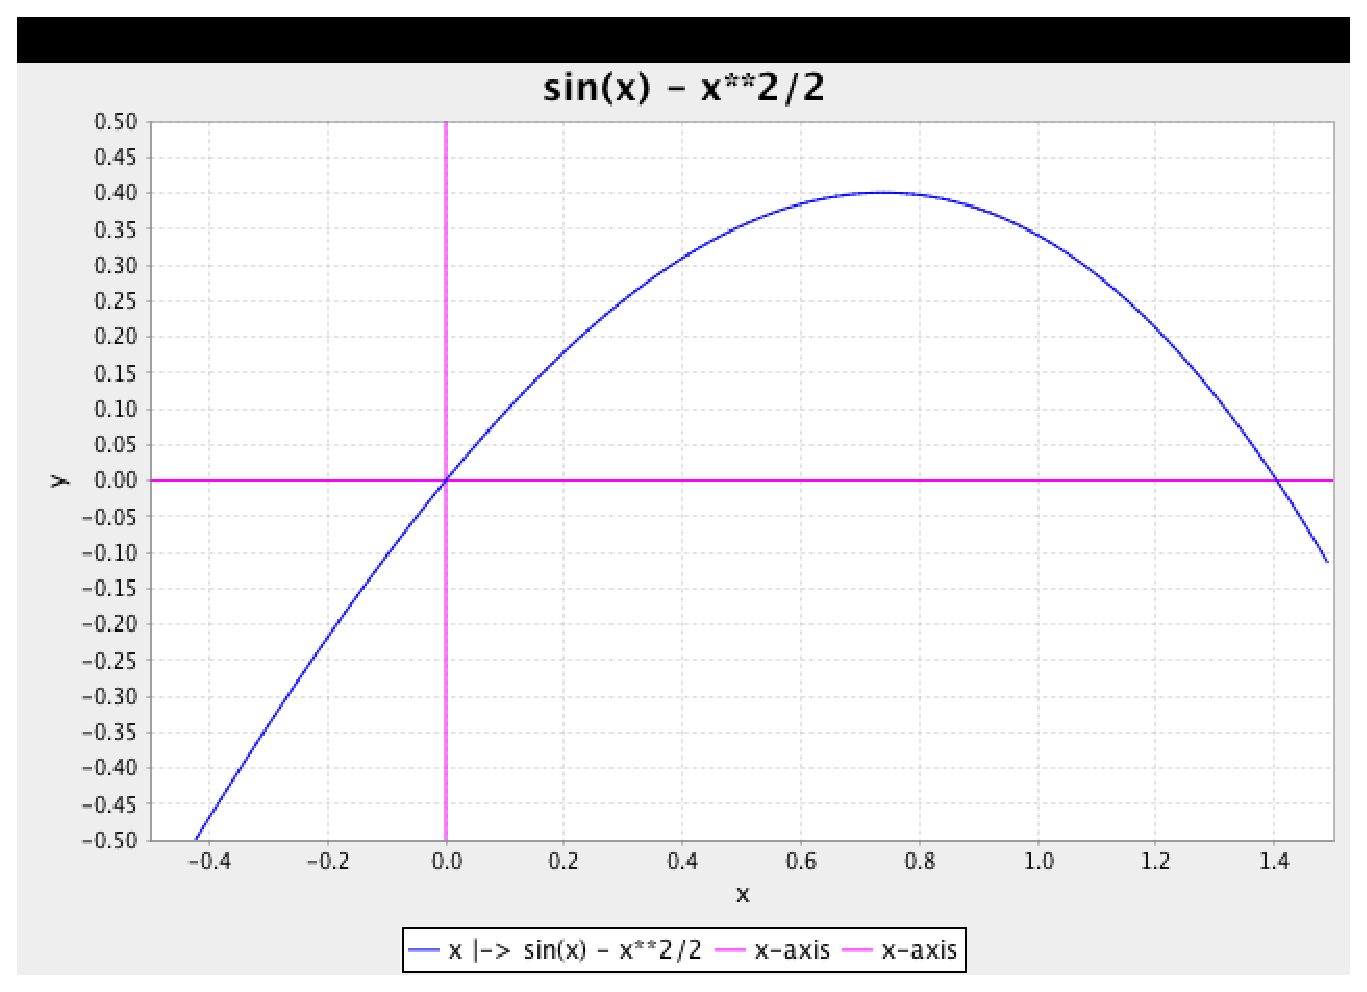
\epsfig{file=Figures/sin-minus-square.eps, scale=0.6}
\vspace*{-0.3cm}
\caption{The function $x \mapsto \sin(x) - \frac{1}{2} \cdot x^2$.}
\label{fig:sin-minus-square.eps}
\end{figure}

\noindent
Unfortunately, in many cases the equation 
\\[0.2cm]
\hspace*{1.3cm}
$\nabla f(\mathbf{\widehat{x}}) = \mathbf{0}$
\\[0.2cm]
can not be solved explicitly.  This is already true in the one-dimensional case, i.e.~if $n=1$.  For example, consider
the function $f:\mathbb{R} \rightarrow \mathbb{R}$ that is defined as
\\[0.2cm]
\hspace*{1.3cm}
$\ds f(x) := \sin(x) - \frac{1}{2} \cdot x^2$.
\\[0.2cm]
This function is shown in Figure \ref{fig:sin-minus-square.eps} on page \pageref{fig:sin-minus-square.eps}.
From the graph of the function it is obvious that this function has a maximum somewhere between $0.6$ and
$0.8$.  In order to compute this maximum, we can compute the derivative of $f$.   This derivative is given as 
\\[0.2cm]
\hspace*{1.3cm}
$f'(x) = \cos(x) - x$
\\[0.2cm]
As it happens, the equation $\cos(x) - x = 0$ does not seem to have a solution in 
\href{https://en.wikipedia.org/wiki/Closed-form_expression}{closed form}.  Hence, we can only approximate
the solution numerically.


The method of \href{https://en.wikipedia.org/wiki/Gradient_descent}{gradient ascent} is a numerical
method that can be used to find the maximum of a function 
\\[0.2cm]
\hspace*{1.3cm}
$f: \mathbb{R}^n \rightarrow \mathbb{R}$.
\\[0.2cm]
The basic idea is to take a vector $\mathbf{x}_0 \in \mathbb{R}^n$ as start value and define a sequence of
vectors $\bigl(\mathbf{x}_n\bigr)_{n\in\mathbb{N}}$ such that we have
\\[0.2cm]
\hspace*{1.3cm}
$f(\mathbf{x}_{n+1}) \geq f(\mathbf{x}_{n})$ \quad for all $n\in\mathbb{N}$.
\\[0.2cm]
Hopefully, this sequence will converge against $\widehat{\mathbf{x}} = \arg\max\limits_{\mathbf{x}\in \mathbb{R}}f(\mathbf{x})$.
If we do not really know where to start our search, we define $\mathbf{x}_0 := \mathbf{0}$.  In order to
compute $\mathbf{x}_{n+1}$ given $\mathbf{x}_{n}$, the idea is to move from $\mathbf{x}_n$ in that direction
where we have the biggest change in the values of $f$.   This direction happens to be the gradient of $f$ at $\mathbf{x}_n$.
Therefore, the definition of $\mathbf{x}_{n+1}$ is given as follows:
\\[0.2cm]
\hspace*{1.3cm}
$\mathbf{x}_{n+1} := \mathbf{x}_n + \alpha \cdot \nabla f(\mathbf{x}_n)$ \quad for all $n \in \mathbb{N}_0$.
\\[0.2cm]
Here, $\alpha$ is called the \blue{step size}.  It determines by how much we move in the direction of the gradient.
In practice, it is best to adapt the step size dynamically during the iteration.  Figure
\ref{fig:gradient-ascent.stlx} shows how this is done.



\begin{figure}[!ht]
\centering
\begin{Verbatim}[ frame         = lines, 
                  framesep      = 0.3cm, 
                  firstnumber   = 1,
                  labelposition = bottomline,
                  numbers       = left,
                  numbersep     = -0.2cm,
                  xleftmargin   = 0.8cm,
                  xrightmargin  = 0.8cm,
                ]
    findMaximum := procedure(f, gradF, start, eps) {
        x     := start;
        fx    := f(x);
        alpha := 1.0;
        while (true) {
            [xOld, fOld] := [x, fx];
            x  += alpha * gradF(x);
            fx := f(x);
            if (fx < fOld) {   
                alpha   *= 0.5;
                [x, fx] := [xOld, fOld];
                continue;  // start over
            } else {
                alpha *= 1.2;
            }
            if (abs(fx - fOld) <= abs(fx) * eps) {
                return [x, fx];
            } 
        }
    };
\end{Verbatim}
\vspace*{-0.3cm}
\caption{The gradient ascent algorithm.}
\label{fig:gradient-ascent.stlx}
\end{figure}

\noindent
The function \texttt{findMaximum} takes four arguments:
\begin{enumerate}
\item \texttt{f} is the function that is to be maximized.  It is assumed that \texttt{f} takes a vector
      $\texttt{x}\in \mathbb{R}^n$ as its input and that it returns a real number.
\item \texttt{gradF} is the gradient of \texttt{f}.  It takes a vector
      $\texttt{x}\in \mathbb{R}^n$ as its input and returns the vector $\nabla \mathtt{f}(\mathtt{x})$.
\item \texttt{start} is the a vector from $\mathbb{R}^n$ that is used as the value of $\mathbf{x}_0$.  In
      practice, we will often use $\mathbf{0} \in \mathbb{R}^n$ as the start vector.
\item \texttt{eps} is the precision that we need for the maximum.  We will have to say more on how \texttt{eps}
      is exactly related to the precision later.  As we are using double precision floating point arithmetic, 
      it won't make sense to use a value for \texttt{eps} that is smaller than $10^{-15}$.
\end{enumerate}
Next, let us discuss the implementation of gradient ascent.
\begin{enumerate}
\item \texttt{x} is initialized with the parameter \texttt{start}.  Hence, \texttt{start} is really the same as
      $\mathbf{x}_0$. 
\item \texttt{fx} is the value that the function $f$ takes for the argument \texttt{x}.
\item \texttt{alpha} is the step size $\alpha$.  We initialize \texttt{alpha} as $1.0$.  It will be adapted
      dynamically. 
\item The \texttt{while} loop starting in line 5 executes the iteration.
\item In each iteration, we store the values of $\mathbf{x}_n$ and $f(\mathbf{x}_n)$ in the variables
      \texttt{xOld} and \texttt{fOld}.
\item Next, we compute $\mathbf{x}_{n+1}$ in line 7 and compute the corresponding value $f(\mathbf{x}_{n+1})$ in line 8.
\item If we are unlucky, $f(\mathbf{x}_{n+1})$ is smaller than $f(\mathbf{x}_{n})$.  This happens if the step
      size $\alpha$ is too large.  Hence, in this case we decrease the value of $\alpha$, discard 
      both $\mathbf{x}_{n+1}$ and $f(\mathbf{x}_{n+1})$ and start over again.
\item Otherwise, $\mathbf{x}_{n+1}$ is a better approximation of the maximum than $\mathbf{x}_n$.  
      In order to increase the speed of the convergence of our algorithm we will then increase the step size
      $\alpha$ by $20\%$.    
\item The idea of our implementation is to stop the iteration when the function values of 
      $f(\mathbf{x}_{n+1})$ and $f(\mathbf{x}_{n})$ do not differ by more than $\varepsilon$ percent, or, to be more
      precise, if
      \\[0.2cm]
      \hspace*{1.3cm}
      $f(\mathbf{x}_{n+1}) < f(\mathbf{x}_{n}) \cdot (1 + \varepsilon)$.
      \\[0.2cm]
      As the sequence $\bigl(f(\mathbf{x}_n\bigr)_{n\in\mathbb{N}}$ will be monotonically
      increasing, i.e.~we have
      \\[0.2cm]
      \hspace*{1.3cm}
      $f(\mathbf{x}_{n+1}) \geq f(\mathbf{x}_{n})$ \quad for all $n\in\mathbb{N}$,
      \\[0.2cm]
      the condition given above is sufficient.  Now, if the increase of  $f(\mathbf{x}_{n+1})$ is less than $f(\mathbf{x}_{n}) \cdot (1 + \varepsilon)$ 
      we assume that we have reached the maximum with the required precision.  In this case we return both the
      value of \texttt{x} and the corresponding function value $f(\mathtt{x})$.
\end{enumerate}
The implementation of gradient ascent given above is not the most sophisticated variant of this algorithm.
It should also be noted that there are algorithms that are more powerful than
gradient ascent.  The first of these methods is the
\href{https://en.wikipedia.org/wiki/Conjugate_gradient_method}{conjugate gradient method}.  A
refinement of this method is the
\href{https://en.wikipedia.org/wiki/Broyden-Fletcher-Goldfarb-Shanno_algorithm}{BFGS-algorithm} that
has been invented by Broyden, Fletcher, Goldfarb, and Shanno.  Unfortunately, we do not have the
time to discuss this algorithm.
However, our implementation of gradient ascent is sufficient for our applications and as this is not a course on numerical
analysis but rather on artificial intelligence we will not delve deeper into this topic but, instead, we refer
readers interested in more efficient algorithms to the literature \cite{snyman:2005}.  If you ever need to find
the maximum of a function numerically, you should try to use a predefined library routine that implements a
state of the art algorithm.


\section{Logistic Regression}
In \href{https://en.wikipedia.org/wiki/Logistic_regression}{logistic regression} we use a linear model that is combined
with the \blue{sigmoid function}.  Before we can discuss the details of logistic regression we need to
define this function and state some of its properties. 

\subsection{The Simoid Function}
\begin{Definition}[Sigmoid Function]
The \href{https://en.wikipedia.org/wiki/Sigmoid_function}{sigmoid function} $S: \mathbb{R} \rightarrow [0, 1]$ is defined as 
\\[0.2cm]
\hspace*{1.3cm}
$\ds S(t) = \frac{1}{1 + \exp(-t)}$.  
\\[0.2cm]
Figure \ref{fig:sigmoid.eps} on page \pageref{fig:sigmoid.eps} shows the sigmoid function.
\eox
\end{Definition}

\begin{figure}[!ht]
\centering
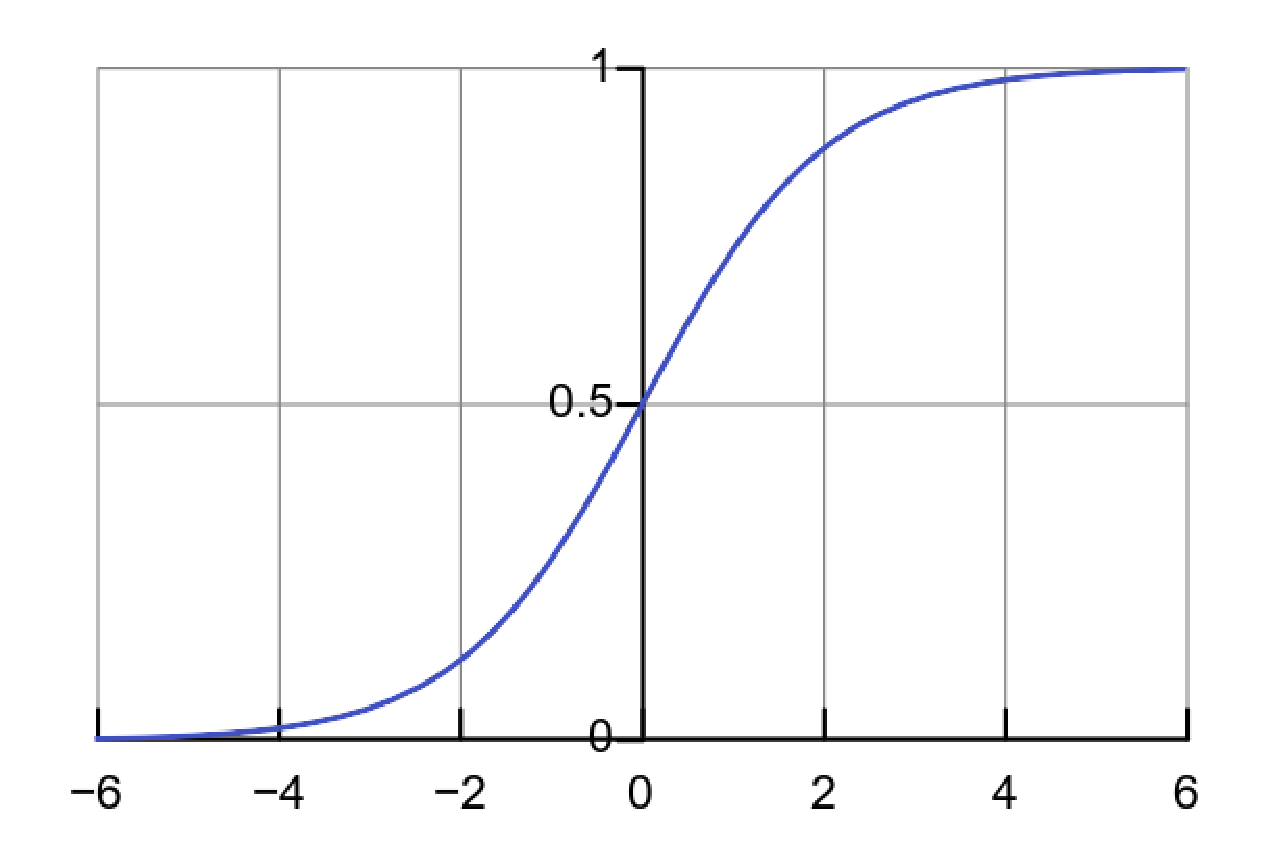
\epsfig{file=Figures/sigmoid.eps, scale=0.7}
\vspace*{-0.3cm}
\caption{The sigmoid function.}
\label{fig:sigmoid.eps}
\end{figure}


\noindent
Let us note some immediate consequences of the definition of the sigmoid function.  As we have
\\[0.2cm]
\hspace*{1.3cm}
$\ds\lim\limits_{x\rightarrow-\infty} \exp(-x) = \infty$, \quad 
$\ds\lim\limits_{x\rightarrow+\infty} \exp(-x) = 0$, \quad and \quad
$\ds\lim\limits_{x\rightarrow\infty} \frac{1}{x} = 0$, 
\\[0.2cm]
the sigmoid function has the following properties:
\\[0.2cm]
\hspace*{1.3cm}
$\ds \lim_{t\rightarrow-\infty} S(t) = 0$ \quad and \quad
$\ds \lim_{t\rightarrow+\infty} S(t) = 1$.
\\[0.2cm]
Another important property is the symmetry of the sigmoid function.  Figure \ref{fig:sigmoid.eps} shows that if the
sigmoid function is shifted down by $\frac{1}{2}$, the resulting function is 
\href{https://en.wikipedia.org/wiki/Point_reflection}{centrally symmetric}, i.e.~we have
\\[0.2cm]
\hspace*{1.3cm}
$\ds S(-t) - \frac{1}{2} = -\Bigl(S(t) - \frac{1}{2}\Bigr)$.
\\[0.2cm]
Adding $\ds\frac{1}{2}$ on both sides of this equation shows that this is equivalent to the equation
\\[0.2cm]
\hspace*{1.3cm}
\colorbox{red}{\framebox{\colorbox{orange}{
$S(-t) = 1 - S(t)$,}}}
\\[0.2cm]
The proof of this fact runs as follows:
\\[0.2cm]
\hspace*{1.3cm}
$
\begin{array}{lcll}
1 - S(t) & = & \ds 1 - \frac{1}{1 + \exp(-t)}             & \mbox{by definition of $S(t)$}           \\[0.5cm]
         & = & \ds \frac{1 + \exp(-t) - 1}{1 + \exp(-t)}  & \mbox{common denominator}                \\[0.5cm]
         & = & \ds \frac{\exp(-t)}{1 + \exp(-t)}          & \mbox{simplify}                          \\[0.5cm]
         & = & \ds \frac{1}{1 + \exp(+t)}                 & \mbox{expand fraction by $\exp(t)$}      \\[0.5cm]
         & = & S(-t). \qquad _\Box                         & \mbox{by definition of $S(-t)$}
\end{array}
$
\\[0.2cm]
The exponential function can be expressed via the sigmoid function.  Let us start with the definition of the sigmoid
function. 
\\[0.2cm]
\hspace*{1.3cm}
$\ds S(t) = \frac{1}{1 + \exp(-t)}$
\\[0.2cm]
Multiplying this equation with the denominator yields
\\[0.2cm]
\hspace*{1.3cm}
$\ds S(t) \cdot \bigl(1 + \exp(-t)\bigr) = 1$.
\\[0.2cm]
Dividing both sides by $S(t)$ gives:
\\[0.2cm]
\hspace*{1.3cm}
$
\begin{array}{cl}
                & \ds 1 + \exp(-t) = \frac{1}{S(t)}        \\[0.5cm]
\Leftrightarrow & \ds \exp(-t) = \frac{1}{S(t)} - 1        \\[0.5cm]
\Leftrightarrow & \ds \exp(-t) = \frac{1 - S(t)}{S(t)}      
\end{array}
$
\\[0.2cm]
We highlight this formula, as we need it later
\\[0.2cm]
\hspace*{1.3cm}
\colorbox{red}{\framebox{\colorbox{orange}{$\ds \exp(-t) = \frac{1 - S(t)}{S(t)}$.}}}
\\[0.2cm]
If we take the reciprocal of both sides of this equation, we have
\\[0.2cm]
\hspace*{1.3cm}
$\ds \exp(t) = \frac{S(t)}{1 - S(t)}$.
\\[0.2cm]
Applying the natural logarithm on both sides of this equation yields
\\[0.2cm]
\hspace*{1.3cm}
$\ds t = \ln\Bigl(\frac{S(t)}{1-S(t)}\Bigr)$.
\\[0.2cm]
This shows that the inverse of the sigmoid function is given as
\\[0.2cm]
\hspace*{1.3cm}
\colorbox{red}{\framebox{\colorbox{orange}{
$\ds S^{-1} (y) = \ln\Bigl(\frac{y}{1-y}\Bigr)$.}}} 
\\[0.2cm]
This function is known as the \href{https://en.wikipedia.org/wiki/Logit}{logit function}.
Next, let us compute the derivative of $S(t)$, i.e.~$\ds S'(t) =\frac{\mathrm{d}S}{\mathtt{d}t}$.  We have
\\[0.2cm]
\hspace*{1.3cm}
$
\begin{array}{lcl}
 S'(t) & = & \ds -\frac{-\exp(-t)}{\bigr(1+\exp(-t)\bigr)^2}   \\[0.5cm]
       & = & \ds \exp(-t) \cdot S(t)^2                       \\[0.2cm]
       & = & \ds \frac{1-S(t)}{S(t)} \cdot S(t)^2            \\[0.4cm]
       & = & \ds \bigl(1 - S(t)\bigr) \cdot S(t)            
\end{array}
$
\\[0.2cm]
We have shown
\\[0.2cm]
\hspace*{1.3cm}
\colorbox{red}{\framebox{\colorbox{orange}{$S'(t) = \bigl(1 - S(t)\bigr) \cdot S(t)$.}}}
\\[0.2cm]
We will later need the derivative of the logarithm of the logistic function.  We define
\\[0.2cm]
\hspace*{1.3cm}
$L(t) := \ln\bigl(S(t)\bigr)$.
\\[0.2cm]
Then we have
\\[0.2cm]
\hspace*{1.3cm}
$
\begin{array}{lcll}
  L'(t) & = & \ds \frac{S'(t)}{S(t)}                  & \mbox{by the chain rule} \\[0.5cm]
        & = & \ds \frac{(1 - S(t)) \cdot S(t)}{S(t)}  \\[0.5cm]
        & = & \ds 1 - S(t)                            \\[0.2cm]
        & = & \ds S(-t)
\end{array}
$
\\[0.2cm]
% If we have the function $f(t) := L(-t)$, then we see that
%\\[0.2cm]
%\hspace*{1.3cm}
% $f'(t) = -S(t)$
%\\[0.2cm]
% holds.   
As this is our most important result, we highlight it:
\\[0.2cm]
\hspace*{1.3cm}
\colorbox{red}{\framebox{\colorbox{orange}{$L'(t) = S(-t)$ \quad where \quad $L(t) := \ln\bigl(S(t)\bigr)$.}}}


\subsection{The Model of Logistic Regression}
We use the following model to compute the probability that an object with features $\mathbf{x}$ will be of the given class:
\\[0.2cm]
\hspace*{1.3cm}
$P(y=+1\;|\;\mathbf{x};\mathbf{w}) = S(\mathbf{x} \cdot \mathbf{w})$.
\\[0.2cm]
Here $\mathbf{x} \cdot \mathbf{w}$ denotes the dot product of the vectors $\mathbf{x}$ and $\mathbf{y}$.  
Seeing this model the first time you might think that this model is not very general and that it can only be
applied in very special circumstances.  However, the fact is that the features can be functions of arbitrary complexity
and hence this model is much more general than it appears on first sight.

As $y$ can only take the values $+1$ or $-1$ and complementary probabilities add up to $1$, we have
\\[0.2cm]
\hspace*{1.3cm}
$P(y=-1\;|\;\mathbf{x};\mathbf{w}) = 1 - P(y=+1\;|\;\mathbf{x};\mathbf{w}) 
  = 1 - S(\mathbf{x} \cdot \mathbf{w}) = S(-\mathbf{x} \cdot \mathbf{w})
$.
\\[0.2cm]
Hence, we can combine the equations for $P(y=-1\;|\;\mathbf{x};\mathbf{w})$ and $P(y=+1\;|\;\mathbf{x};\mathbf{w})$ into a
single equation
\\[0.2cm]
\hspace*{1.3cm}
\colorbox{red}{\framebox{\colorbox{orange}{$P(y\;|\;\mathbf{x};\mathbf{w}) = S\bigl(y \cdot(\mathbf{x} \cdot \mathbf{w})\bigr)$.}}}
\\[0.2cm]
Given $N$ objects $o_1, \cdots, o_n $ with feature vectors $\mathbf{x}_1, \cdots, \mathbf{x}_n$ we
want to determine the weight vector $\mathbf{w}$ such that the likelihood $\ell(\mathbf{X}, \mathbf{y})$ of all of our
observations is maximized.  This approach is called the 
\href{https://en.wikipedia.org/wiki/Maximum_likelihood_estimation}{maximum likelihood estimation} of the weights.
As we assume the probabilities of different objects to be independent, the individual
probabilities have to be multiplied to compute the overall likelihood $\ell(\mathbf{X}, \mathbf{y};\mathbf{w})$ 
of a given training set:
\\[0.2cm]
\hspace*{1.3cm}
$\ds \ell(\mathbf{X},\mathbf{y};\mathbf{w}) = \prod\limits_{i=1}^N P(y_i \;|\;\mathbf{x}_i;\mathbf{w})$.
\\[0.2cm]
Here, we have combined the different attribute vectors $\mathbf{x}_i$ into the matrix $\mathbf{X}$.  Since it is
easier to work with sums than with products, instead of maximizing the function $\ell(\mathbf{X},\mathbf{y};\mathbf{w})$ we maximize the function
\\[0.2cm]
\hspace*{1.3cm}
$\ell\ell(\mathbf{X},\mathbf{y};\mathbf{w}) := \ln\bigl(\ell(\mathbf{X},\mathbf{y};\mathbf{w})\bigr)$. 
\\[0.2cm]
As the natural logarithm is a monotone function, the functions $\ell(\mathbf{X},\mathbf{y};\mathbf{w})$ and 
$\ell\ell(\mathbf{X},\mathbf{y};\mathbf{w})$ take their maximum at the same value of $\mathbf{w}$.  Since we have
\\[0.2cm]
\hspace*{1.3cm}
$\ln(a \cdot b) = \ln(a) + \ln(b)$,
\\[0.2cm]
the natural logarithm of the likelihood is 
\\[0.2cm]
\hspace*{1.3cm}
\colorbox{red}{\framebox{\colorbox{orange}{
$\ds \ell\ell(\mathbf{X},\mathbf{y};\mathbf{w}) = 
 \sum\limits_{i=1}^N \ln\Bigl(S\bigl(y_i \cdot(\mathbf{x}_i \cdot \mathbf{w})\bigr)\Bigr) =
 \sum\limits_{i=1}^N L\bigl(y_i \cdot(\mathbf{x}_i \cdot \mathbf{w})\bigr)
$.}}}
\\[0.2cm]
Our goal is to maximize the likelihood.  Since this is the same as maximizing the log-likelihood, we
need to determine those values of the coefficients $\mathbf{w}$ that satisfy
\\[0.2cm]
\hspace*{1.3cm}
$\ds \frac{\partial\quad}{\partial\, w_j}\ell\ell(\mathbf{X},\mathbf{y};\mathbf{w}) = 0$.
\\[0.2cm]
In order to compute the partial derivative of $\ell\ell(\mathbf{X},\mathbf{y};\mathbf{w})$ with respect to the
coefficients $\mathbf{w}$ we need to compute the partial derivative of the dot product $\mathbf{x}_i \cdot \mathbf{w}$.
We define
\\[0.2cm]
\hspace*{1.3cm}
$\ds h(\mathbf{w}) := \mathbf{x}_i \cdot \mathbf{w} = \sum\limits_{j=1}^D x_{i,j} \cdot w_j$.
\\[0.2cm]
Then we have
\\[0.2cm]
\hspace*{1.3cm}
$\ds \frac{\partial\quad}{\partial\, w_j} h(\mathbf{w}) = x_{i,j}$.
\\[0.2cm]
Now we are ready to compute the partial derivative of $\ell\ell(\mathbf{X},\mathbf{y};\mathbf{w})$ with respect to $\mathbf{w}$:
\\[0.2cm]
\hspace*{1.3cm}
$
\begin{array}{cl}
  & \ds \frac{\partial\quad}{\partial\, w_j} \ell\ell(\mathbf{X},\mathbf{y};\mathbf{w}) \\[0.5cm]
= & \ds \frac{\partial\quad}{\partial\, w_j} 
    \sum\limits_{i=1}^N L\bigl(y_i \cdot(\mathbf{x}_i \cdot \mathbf{w})\bigr) 
    \\[0.5cm]
= & \ds\sum\limits_{i=1}^N y_i \cdot x_{i,j} \cdot  S\bigl(-y_i \cdot(\mathbf{x}_i \cdot \mathbf{w})\bigr)
\end{array}
$
\\[0.2cm]
Hence, the partial derivative of the log-likelihood function is given as follows:
\\[0.2cm]
\hspace*{1.3cm}
\colorbox{red}{\framebox{\colorbox{orange}{
$\ds \frac{\partial\quad}{\partial\, w_j}\ell\ell(\mathbf{X},\mathbf{y};\mathbf{w}) =
 \ds\sum\limits_{i=1}^N y_i \cdot x_{i,j} \cdot  S(-y_i \cdot \mathbf{x}_i \cdot \mathbf{w})
$}}} 
\\[0.2cm]
Next, we have to find the value of $\mathbf{w}$ such that
\\[0.2cm]
\hspace*{1.3cm}
$\ds\sum\limits_{i=1}^N y_i \cdot x_{i,j} \cdot  S(-y_i \cdot \mathbf{x}_i \cdot \mathbf{w}) = 0$
\quad for all $j \in \{1, \cdots, D\}$.
\\[0.2cm]
These are $D$ equation for the $D$ variables $w_1, \cdots w_D$.  Due to the occurrence of the sigmoid function, these
equations are nonlinear.  In order to find the value of $\mathbf{w}$ that maximizes the likelihood, we will instead use
the method of \href{https://en.wikipedia.org/wiki/Gradient_descent}{gradient ascent} to compute
the best value of $\mathbf{w}$.  This method has been outlined in the previous section.

\subsection{Implementing Logistic Regression}
In order to implement logistic regression we need a data structure for tabular data.  Figure
\ref{fig:table.stlx} on page \pageref{fig:table.stlx} shows the class table that can be used to
administer this kind of data.  Figure \ref{fig:table.stlx}  shows an example of tabular data that is
stored in a \href{https://en.wikipedia.org/wiki/Comma-separated_values}{csv file}.  In this case,
the data stores the hours a student has learned for a particular exam and the fact whether the
student has passed of failed.  The first column stores pass or fail, where a pass is coded using the
number 1, while a fail is coded as 0.  The second column stores the number of hours that the student
has learned in order to pass the exam.

\begin{figure}[!ht]
\centering
\begin{Verbatim}[ frame         = lines, 
                  framesep      = 0.3cm, 
                  firstnumber   = 1,
                  labelposition = bottomline,
                  numbers       = left,
                  numbersep     = -0.2cm,
                  xleftmargin   = 0.8cm,
                  xrightmargin  = 0.8cm,
                ]
   class table(columnNames, types, data) {
       mColumnNames := columnNames;
       mTypes       := types;
       mData        := data;
   
     static {
         getColumnNames := [ ] |-> mColumnNames;
         getTypes       := [ ] |-> mTypes;
         getData        := [ ] |-> mData;
         getRow         := [r] |-> mData[r];
         getLength      := []  |-> #mData;
         
         head := procedure(limit := 10) {
             print(mColumnNames);
             print(mTypes);
             for (i in [1 .. limit]) {
                 print(mData[i]);
             }
         };
     }
   }
   readTable := procedure(fileName, types) {
       all := readFile(fileName);
       columnNames := split(all[1], ',\s*');
       data := [];
       for (i in [2 .. #all]) {
           row := split(all[i], ',\s*');
           data[i-1] := [eval("$type$($s$)") : [type, s] in types >< row];
       }
       return table(columnNames, types, data);
   };
\end{Verbatim}
\vspace*{-0.3cm}
\caption{A class to represent tabular data.}
\label{fig:table.stlx}
\end{figure}
There is no need for us to discuss every detail of the implementation of the class \texttt{table}.
The important thing to note is that the data is stored as a list of lists in the member variable
\texttt{mData}.  Each of the inner lists corresponds to one row of the csv file.
This member variable can be accessed using the function getData.  The function \texttt{readTable}
has the responsibility to read a csv file and to convert it into an object of class \texttt{table}.
In order to do this, it has to be called with two arguments.  The first argument is the file name,
the second argument is a list of the types of each column in the csv file.  For example, to read the
file ``\texttt{exam.csv}'' we would call \texttt{readTable} as follows:
\\[0.2cm]
\hspace*{1.3cm}
\texttt{readTable("exam.csv", ["int", "double"])}.



\begin{figure}[!ht]
\centering
\begin{Verbatim}[ frame         = lines, 
                  framesep      = 0.3cm, 
                  firstnumber   = 1,
                  labelposition = bottomline,
                  numbers       = left,
                  numbersep     = -0.2cm,
                  xleftmargin   = 0.8cm,
                  xrightmargin  = 0.8cm,
                ]
   Pass, Hours
   0,    0.50
   0,    0.75
   0,    1.00
   0,    1.25
   0,    1.50
   0,    1.75
   1,    1.75
   0,    2.00
   1,    2.25
   0,    2.50
   1,    2.75
   0,    3.00
   1,    3.25
   0,    3.50
   1,    4.00
   1,    4.25
   1,    4.50
   1,    4.75
   1,    5.00
   1,    5.50
\end{Verbatim}
\vspace*{-0.3cm}
\caption{Results of an exam.}
\label{fig:exam.csv}
\end{figure}

The program shown in Figure \ref{fig:logistic-regression.stlx} on page
\pageref{fig:logistic-regression.stlx} implements logistic regression.  As there are a number of
subtle points that might easily be overlooked otherwise, we proceed to discuss this program line by line. 


\begin{figure}[!ht]
\centering
\begin{Verbatim}[ frame         = lines, 
                  framesep      = 0.3cm, 
                  firstnumber   = 1,
                  labelposition = bottomline,
                  numbers       = left,
                  numbersep     = -0.2cm,
                  xleftmargin   = 0.8cm,
                  xrightmargin  = 0.8cm,
                ]
   load("table.stlx");
   load("gradient-ascent.stlx");
   
   sigmoid := procedure(x) { return 1.0 / (1.0 + exp(-x)); };
   logSigmoid := procedure(x) {
       if (x >= -100) {
           return -log(1.0 + exp(-x));
       } else {  
           return x;
       }
   };
   ll := procedure(x, y, w) {
       result := 0;
       for (i in [1 .. #x]) {
           result += logSigmoid(y[i] * (x[i] * w));
       }
       return result;
   };   
   gradLL := procedure(x, y, w) {
       result := [];
       for (j in [1 .. #x[1]]) {
           result[j] := 0;
           for (i in [1 .. #x]) {
               result[j] += y[i] * x[i][j] * sigmoid((-y[i]) * (x[i] * w));
           }
       }
       return la_vector(result);
   };
   logisticRegressionFile := procedure(fileName, types) {
       csv    := readTable(fileName, types);
       data   := csv.getData();
       number := #data;
       dmnsn  := #data[1];    
       yList  := [];
       xList  := [];
       for (i in [1 .. number]) {
           yList[i] := data[i][1];
           xList[i] := la_vector([1.0] + data[i][2..]);
       }
       x := la_matrix(xList);
       y := la_vector([2 * y - 1 : y in yList]);
       start := la_vector([0.0 : i in [1 .. dmnsn]]);
       eps   := 10 ** -15;
       f     := w |=> ll(x, y, w);
       gradF := w |=> gradLL(x, y, w);
       return findMaximum(f, gradF, start, eps)[1];
   };
\end{Verbatim}
\vspace*{-0.3cm}
\caption{An implementation of logistic regression.}
\label{fig:logistic-regression.stlx}
\end{figure}

\begin{enumerate}
\item First, we have to load both the class \texttt{table} and our implementation of gradient ascent 
      that has already been discussed in Section \ref{section:gradient-ascent}.
\item Line 4 implements the sigmoid function
      \\[0.2cm]
      \hspace*{1.3cm}
      $\ds S(x) = \frac{1}{1 + \exp(-x)}$.
\item Line 5 starts the implementation of the natural logarithm of the sigmoid function, i.e.~we implement
      \\[0.2cm]
      \hspace*{1.3cm}
      $\ds L(x) = \ln\bigl(S(X)\bigr) = \ln\Bigl(\frac{1}{1 + \exp(-x)}\Bigr) =- \ln\bigl(1 + \exp(-x)\bigr)$.
      \\[0.2cm]
      The implementation is more complicated than you might expect.  The reason has to do with
      overflow.  Consider values of $x$ that are smaller than, say, $-1000$.  The problem is that
      the expression $\mathtt{exp}(1000))$ evaluates to \texttt{Infinity}, which represents the
      mathematical value $\infty$.  But then $1 + \mathtt{exp}(1000))$ is also \texttt{Infinity} and
      finally \texttt{log(1 + exp(1000))} is \texttt{Infinity}.  However, in reality we have
      \\[0.2cm]
      \hspace*{1.3cm}
      $\ln\bigl(1 + \exp(1000)\bigr) \approx 1000$.
      \\[0.2cm] 
      The argument works as follows:
      \\[0.2cm]
      \hspace*{1.3cm}
      $
      \begin{array}{lcll}
        \ln\bigl(1+\exp(x)\bigr) & = & \ln\bigl(\exp(x) \cdot (1+\exp(-x))\bigr)          \\[0.2cm]
                                 & = & \ln\bigl(\exp(x)\bigr) + \ln\bigl(1+\exp(-x)\bigr) \\[0.2cm]
                                 & = & x + \ln\bigl(1+\exp(-x)\bigr) \\[0.2cm]
                                 & \approx & x + \ln(1) + \exp(-x) & \mbox{Taylor expansion of $\ln(1+x)$} \\[0.2cm]
                                 & = & x + 0 + \exp(-x)                                      \\[0.2cm]
                                 & \approx & x                & \mbox{since $\exp(-x) \approx 0$ for large $x$} 
      \end{array}
      $
      \\[0.2cm]
      This is the reason that \texttt{logSigmoid} returns \texttt{x} if \texttt{x} is less than
      $-100$.
\item The function $\mathtt{ll}(\mathbf{x}, \mathbf{y}, \mathbf{w})$ computes the log-lokelihood
      $\ds \ell\ell(\mathbf{X},\mathbf{y};\mathbf{w}) = 
           \sum\limits_{i=1}^N L\bigl(y_i \cdot(\mathbf{x}_i \cdot \mathbf{w})\bigr)
      $.
      Here $L$ denotes the natural logarithm of the sigmoid of the argument.
      It is assumed that \texttt{x} is a matrix.  Every observation corresponds to a row in this
      matrix, i.e.~the vector $\mathbf{x}_i$ is the feature vector containing the features of the
      $i$-th observation.  $\mathbf{y}$ is a vector describing the outcomes, i.e.~the elements
      of this vector are either $+1$ or $-1$.  Finally, $\mathbf{w}$ is the vector of coefficients.
\item The function $\mathtt{gradLL}(\mathbf{x}, \mathbf{y}, \mathbf{w})$ computes the gradient of
      the log-lokelihood according to the formula
      \\[0.2cm]
      \hspace*{1.3cm}
      $\ds \frac{\partial\quad}{\partial\, w_j}\ell\ell(\mathbf{X},\mathbf{y};\mathbf{w}) =
        \ds\sum\limits_{i=1}^N y_i \cdot x_{i,j} \cdot  S(-y_i \cdot \mathbf{x}_i \cdot \mathbf{w})
      $.
      \\[0.2cm]
      The different components of this gradient are combined into a vector.
      The arguments are the same as the arguments to the log-lokelihood.
\item Finally, the function \texttt{logisticRegressionFile} takes two arguments.  The first argument
      is the name of the csv file containing the data, while the second argument is a list specifying the types
      of the columns.  The elements of this list have to be either \texttt{"int"} or
      \texttt{"double"}.
      The task of this function is to read the csv file, convert the data in the matrix \texttt{x}
      and the vector \texttt{y}, and then use gradient ascent to find the best coefficients.
\end{enumerate}
If we run the function \texttt{logisticRegressionFile} using the data shown in Figure
\ref{fig:exam.csv} via
the command
\\[0.2cm]
\hspace*{1.3cm}
\texttt{logisticRegressionFile("exam.csv", ["int", "double"]);}
\\[0.2cm]
the resulting coefficients are:
\\[0.2cm]
\hspace*{1.3cm}
\texttt{<<-4.077649741107752 1.5046211108850898>>}
\\[0.2cm]
This shows that the probability $P(h)$ that a student who has studied for $h$ hours will pass the
exam is given approximately as follows:
\\[0.2cm]
\hspace*{1.3cm}
$\ds P(h) \approx \frac{1}{1 + \exp(4.1 - 1.5 \cdot h)}$
\\[0.2cm]
Figure \ref{fig:exam-pass.eps} shows a plot of the probability $P(x)$.  This
figure has been taken from the
\href{https://en.wikipedia.org/wiki/Logistic_regression#Fields_and_example_applications}{Wikipedia article on logistic regression}. 
It has been created by \href{https://commons.wikimedia.org/w/index.php?curid=42442194}{Michaelg2015}.


\begin{figure}[!th]
\centering
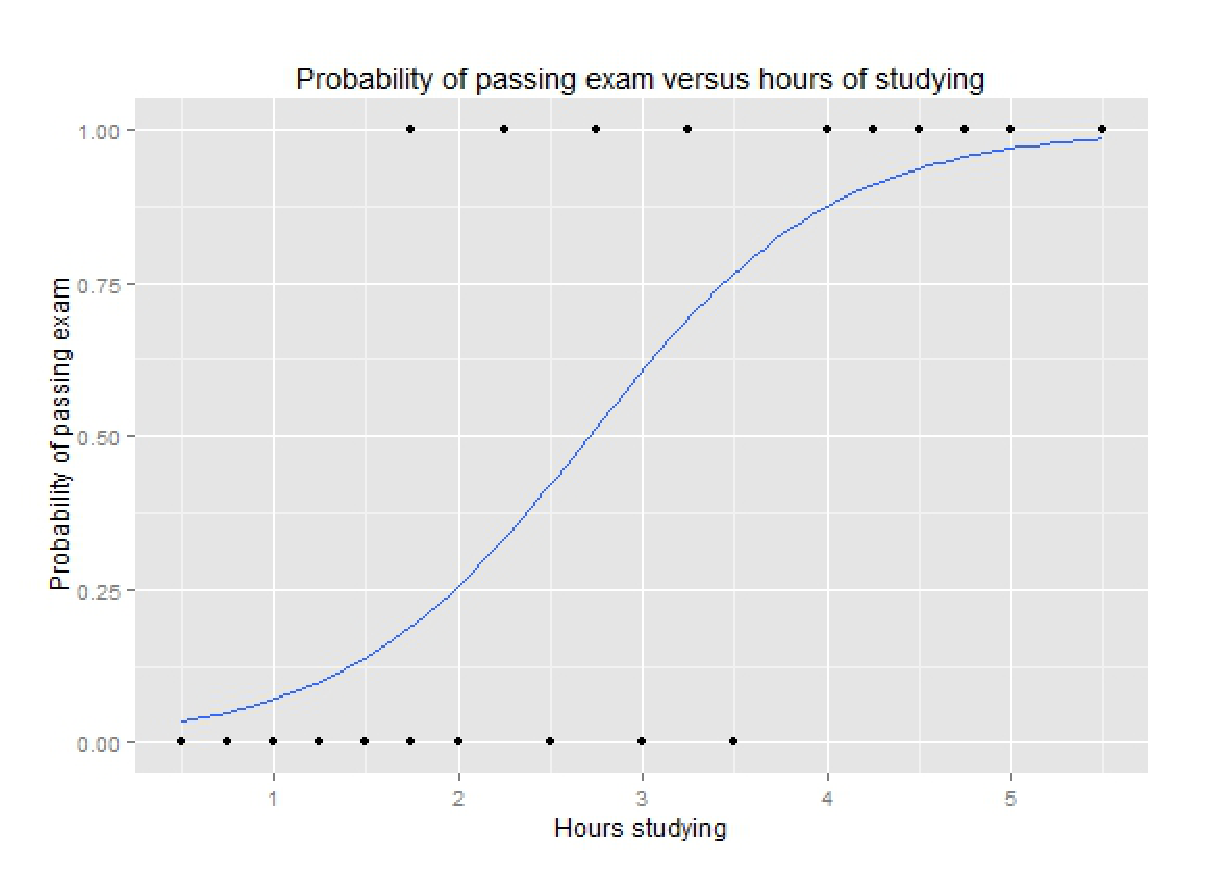
\epsfig{file=Figures/exam-pass.eps, scale=0.6}
\vspace*{-0.3cm}
\caption{Probability of passing an exam versus hours of studying.}
\label{fig:exam-pass.eps}
\end{figure}


%\section{Decision Tree Learning}

%%% Local Variables:
%%% mode: latex
%%% TeX-master: "artificial-intelligence"
%%% End:

\chapter{Neural Networks}
A neural network is built from \emph{neurons}.  At the abstraction level that we are looking at
neural networks, a single neuron with $n$ inputs is defined as a pair $\langle \mathbf{w}, b\rangle$ where
vector $\mathbf{w} \in \mathbb{R}^m$ is called the \emph{weight vector} and $b \in \mathbb{R}$ is called the \emph{bias}.  
Conceptually, a neuron is a function $p$ that maps a vector $\mathbf{x} \in \mathbb{R}^m$ into the
interval $[0,1]$.  This function is defined as follows:
\\[0.2cm]
\hspace*{1.3cm}
$\ds p(\mathbf{x}; \mathbf{w}) := a(\mathbf{x} \cdot \mathbf{w} + b)$,
\\[0.2cm]
where $a$ is called the \emph{activation function}.  In our applications, we will use the sigmoid
function as our activation function, i.e.~we have
\\[0.2cm]
\hspace*{1.3cm}
$\ds a(t) := S(t) = \frac{1}{1 + \exp(-t)}$.
\\[0.2cm]
The function $p$ modeling the neuron can also be written using index notation.  If
\\[0.2cm]
\hspace*{1.3cm}
$\mathbf{w} = \langle w_1, \cdots, w_m \rangle^T$ 
\\[0.2cm]
is the weight vector and 
\\[0.2cm]
\hspace*{1.3cm}
$\mathbf{x} = \langle x_1, \cdots, x_m \rangle^T$
\\[0.2cm]
is the input vector, then 
\\[0.2cm]
\hspace*{1.3cm}
$\ds p(\mathbf{x}; \mathbf{w}) = S\left(\sum\limits_{i=1}^m x_i \cdot w_i + b\right)$
\\[0.2cm]
if we use the sigmoid function as our activation function.  If you compare $p(\mathbf{x}; \mathbf{w})$ 
to a similar function appearing in the last chapter, you will notice 
that so far a neuron works just like logistic regression.  The only difference is that the bias $b$
is now explicit.  

A neural network is a layered network of neurons.  Formally, the \emph{topology} of a neural network is
given by a number $L \in \mathbb{N}$ and a list of $[m(1), \cdots, m(L)]$ of $L$ natural numbers.  The number
$L$ is called the number of layers and for $i \in \{2,\cdots,L\}$ the number $m(i)$ is the number of
neurons in the $l$-th layer.  The first layer is called the input layer, the last layer (i.e.~the
layer with index $L$) is called the output layer and the remaining layers are called 
\emph{hidden layers}.  If there is more than one hidden layer, the neural network is called a
\emph{deep neural network}.

As the first layer is the input layer, the \emph{input dimension} is defined as
$m(1)$.  Similarly, the \emph{output dimension} is defined as $m(L)$.
Every node in the $l$-th layer is connected to every node in the $(l+1)$-th layer.
The weight $w_{j,k}^{(l)}$ is the weight of the connection from the $k$-th neuron in layer $l-1$ to
the $j$-th neuron in layer $l$.  The weights in layer $l$ are combined into the weight matrix of
layer $W^{(l)}$ which is defined as
\\[0.2cm]
\hspace*{1.3cm}
$\ds W^{(l)} := \bigl( w_{j,k}^{(l)} \bigr)$.
\\[0.2cm]
Note that $W^{(l)}$ is an $m(l-1) \times m(l)$ matrix, i.e.~we have
\\[0.2cm]
\hspace*{1.3cm}
$\ds W^{(l)} \in \mathbb{R}^{m(l-1) \times m(l)}$.
\\[0.2cm]
The $j$-th neuron in layer $l$ has the bias $b_j^{(l)}$.  Then, the activation of the $j$-th neuron
in layer $l$ is denoted as $a_j^{(l)}$ and is defined as 
\\[0.2cm]
\hspace*{1.3cm}
$\ds a_j^{(l)} := S\left(\sum\limits_{k=1}^{n(l-1)} w_{j,k}^{(l)}\cdot a^{(l-1)} + b_{j}^{(l)}\right)$.
\\[0.2cm]
The output of our neural network for an input $\mathbf{x}$ is given by the neuron in the output
layer,  i.e.~the output vector 
$\mathbf{o}(\mathbf{x}) \in \mathbb{R}^{(m(L))}$ is defined as 
\\[0.2cm]
\hspace*{1.3cm}
$\mathbf{o}(\mathbf{x}) = \langle a^{(L)}_1(\mathbf{x}), \cdots, a^{(L)}_{m(L)}(\mathbf{x}) \rangle$.
\\[0.2cm]
We assume that we have $n$ training examples 
\\[0.2cm]
\hspace*{1.3cm}
$\langle \mathbf{x}^{(i)}, \mathbf{y}^{(i)} \rangle$ \quad for $i=1,\cdots,n$ 
\\[0.2cm]
such that 
\\[0.2cm]
\hspace*{1.3cm}
$\mathbf{x}^{(i)} \in \mathbb{R}^{m(1)}$ and $\mathbf{y}^{(i)} \in \mathbb{R}^{m(L)}$
\\[0.2cm]
The \emph{quadratic error cost function} is defined as
\\[0.2cm]
\hspace*{1.3cm}
$\ds C\Bigr(W^{(2)}, \cdots, W^{(L)}, \mathbf{b}^{(2)}, \cdots, \mathbf{b}^{(L)};
     \mathbf{x}^{(1)}, \mathbf{y}^{(1)}, \cdots, \mathbf{x}^{(n)},\mathbf{y}^{(n)} \Bigr) := 
 \frac{1}{2 \cdot m} \cdot \sum\limits_{i=1}^n \Bigl(\mathbf{o}\bigl(\mathbf{x}^{(i)}\bigr) - \mathbf{y}^{(i)}\Bigr)^2
$.
\\[0.2cm]
Note that the cost function is additive in the training examples $\langle \mathbf{x}^{(i)}, \mathbf{y}^{(i)} \rangle$.
In order to simplify the notation we therefore define
\\[0.2cm]
\hspace*{1.3cm}
$\ds C_{\mathbf{x}, \mathbf{y}}\Bigr(W^{(2)}, \cdots, W^{(L)}, \mathbf{b}^{(2)}, \cdots, \mathbf{b}^{(L)}\Bigr) := 
 \frac{1}{2} \cdot \Bigl(\mathbf{o}\bigl(\mathbf{x}\bigr) - \mathbf{y}\Bigr)^2
$.
\\[0.2cm]
Then, we have
\\[0.2cm]
$\ds C\Bigr(W^{(2)}, \cdots, W^{(L)}, \mathbf{b}^{(2)}, \cdots, \mathbf{b}^{(L)};
     \mathbf{x}^{(1)}, \mathbf{y}^{(1)}, \cdots, \mathbf{x}^{(n)},\mathbf{y}^{(n)} \Bigr) := 
 \frac{1}{m} \cdot \sum\limits_{i=1}^n C_{\mathbf{x^{(i)}}, \mathbf{y^{(i)}}}\Bigr(W^{(2)}, \cdots W^{(L)}, \mathbf{b}^{(2)}, \cdots, \mathbf{b}^{(L)}\Bigr) 
$.
\\[0.2cm]
As the notation
\\[0.2cm]
\hspace*{1.3cm}
$C_{\mathbf{x}, \mathbf{y}}\Bigr(W^{(2)}, \cdots, W^{(L)}, \mathbf{b}^{(2)}, \cdots, \mathbf{b}^{(L)}\Bigr)$
\\[0.2cm]
is far too heavy, we will abbreviate this term as $C$ in the following
discussion of the backpropagation algorithm.

\section{Backpropagation}
%%% Local Variables:
%%% mode: latex
%%% TeX-master: "artificial-intelligence"
%%% End:

% \chapter{Clustering and Retrieval}


The \emph{inverse document frequency} $\mathtt{idf}(w)$ of a word $w$ with respect to a corpus $C$ is defined as
follows:
\\[0.2cm]
\hspace*{1.3cm}
$\ds\mathtt{idf}(w) := \ln\left(\frac{\cnt C}{1 + \mathtt{count}(w, C)}\right)$.
\\[0.2cm]
Here, $\cnt C$ is the number of documents that are present in the corpus $C$, while
$\mathtt{count}(w, C)$ yields the number of documents in the corpus $C$ that contain the word $w$,
i.e.~we have
\\[0.2cm]
\hspace*{1.3cm}
$\mathtt{count}(w, C) := \cnt\{ d \in C \,|\, w \in d \}$.
\\[0.2cm]

%%% Local Variables:
%%% mode: latex
%%% TeX-master: "artificial-intelligence"
%%% End:


\bibliographystyle{alpha}
\bibliography{cs}
\listoffigures
\printindex

\end{document}

%%% Local Variables:
%%% mode: latex
%%% TeX-master: "artificial-intelligence"
%%% End:
